\pdfcompresslevel=9
\pdfminorversion=5
\pdfobjcompresslevel=2


\documentclass[12pt]{article}
\usepackage{natbib}
\usepackage[flushleft]{threeparttable}
\usepackage{longtable}
\usepackage{bm}
\usepackage{placeins}
\usepackage{caption}

\usepackage[toc,page,header]{appendix}

\usepackage{listings}
\usepackage[english]{babel}
\usepackage[utf8]{inputenc}
\usepackage[dvips]{graphicx}
\usepackage{amsmath,amsthm,amssymb,tipa,dsfont,mathtools,mathrsfs,here,titlesec,fancyhdr}
\usepackage{anysize}
\usepackage{subfigure}
\usepackage{color}
\usepackage{enumerate}
\usepackage{booktabs}
\usepackage{rotating}
\usepackage{parskip} % to avoid // 
\usepackage[hidelinks]{hyperref}
\usepackage{url}
\usepackage{multirow}
\renewcommand{\qedsymbol}{\rule{0.7em}{0.7em}}
\usepackage{comment} % begin{comment} to comment large sections
\usepackage[font=scriptsize]{caption}
\usepackage{rotating} % to rotate tables 
\usepackage{tikz}
\usetikzlibrary{shapes,decorations,arrows,calc,arrows.meta,fit,positioning}
\tikzset{
	-Latex,auto,node distance =1 cm and 1 cm,semithick,
	state/.style ={ellipse, draw, minimum width = 0.7 cm},
	point/.style = {circle, draw, inner sep=0.04cm,fill,node contents={}},
	bidirected/.style={Latex-Latex,dashed},
	el/.style = {inner sep=2pt, align=left, sloped}
}

\definecolor{Grey}{RGB}{150, 150, 150}
\definecolor{PPblue}{RGB}{0,114,198}
\definecolor{VOXblue}{RGB}{0,114,198}
\definecolor{PSOEred}{RGB}{232,0,0}
\definecolor{UPred}{RGB}{232,0,0}
\newcommand{\sym}[1]{\rlap{#1}}

\definecolor{mypink}{rgb}{0.858, 0.188, 0.478}
\definecolor{myorange}{rgb}{1.0, 0.49, 0.0}
\definecolor{mypurple}{rgb}{0.6, 0.4, 0.8}
%\usepackage[colorlinks=true,linkcolor=blue,citecolor=blue,hyperfootnotes=false]{hyperref} 
\hypersetup{
	colorlinks,
	citecolor=blue,
	linkcolor=mypink,
	urlcolor=mypurple}
%Els comandaments següents són per a linkejar (han d'estar al final de tots els usepackage)
%\usepackage[colorlinks]{hyperref}%aquests paquets s'utilitzen per a poder linkejar coses.
%\hypersetup{citecolor=red}
%\hypersetup{linkcolor=red}
%\hypersetup{urlcolor=red}
%\usepackage{cleveref}%aquest també.

\usepackage[T1]{fontenc} % for porper quotation marks 
\PassOptionsToPackage{svgnames}{xcolor}
\usepackage{pgfplots}


\usepackage{tcolorbox}
\usepackage{lipsum}
\tcbuselibrary{skins,breakable}
\usetikzlibrary{shadings,shadows}
\newenvironment{myblock}[1]{%
	\tcolorbox[beamer,%
	noparskip,breakable,
	colback=LightBlue,colframe=DarkBlue,%
	colbacklower=DarkBlue!75!LightBlue,%
	title=#1]}%
{\endtcolorbox}

\usepackage{tikz}
\usetikzlibrary{shapes,decorations,arrows,calc,arrows.meta,fit,positioning}
\tikzset{
	-Latex,auto,node distance =1 cm and 1 cm,semithick,
	state/.style ={ellipse, draw, minimum width = 0.7 cm},
	point/.style = {circle, draw, inner sep=0.04cm,fill,node contents={}},
	bidirected/.style={Latex-Latex,dashed},
	el/.style = {inner sep=2pt, align=left, sloped}
}














\renewcommand{\baselinestretch}{1.2} %separació entre linies
\marginsize{2.3cm}{2.3cm}{1cm}{2cm} %Margens


%ací definim els colors que anem a gastar
\definecolor{secction}{rgb}{0.62,0.31,0.00}
\definecolor{subsection}{rgb}{0.33,0.00,0.33}
\definecolor{mygreen}{RGB}{28,172,0}


%S'utilitza per a insertar programes de forma més professional
%\lstset{language=Matlab,numbers=left,frame=single,title=\lstname}
\lstset{language=Matlab,%
    %basicstyle=\color{red},
    breaklines=true,%
    morekeywords={matlab2tikz},
    keywordstyle=\color{blue},%
    morekeywords=[2]{1}, keywordstyle=[2]{\color{black}},
    identifierstyle=\color{black},%
    %stringstyle=\color{mylilas},
    commentstyle=\color{mygreen},%
    showstringspaces=false,%without this there will be a symbol in the places where there is a space
    numbers=left,%
    numberstyle={\tiny \color{black}},% size of the numbers
    numbersep=9pt, % this defines how far the numbers are from the text
    emph=[1]{for,end,break},emphstyle=[1]\color{blue}, %some words to emphasise
    %emph=[2]{word1,word2}, emphstyle=[2]{style},
}

\usepackage[colorinlistoftodos,textwidth=3cm]{todonotes}
\newcommand{\todoINFO}[1]{\todo[color=blue!25]{INFO: #1}}
\newcommand{\todoIMPORTANT}[1]{\todo[color=red!25]{IMPORTANT: #1}}
\newcommand{\todoREV}[1]{\todo[color=green!25]{REVIEWED: #1}}
%Aquí redefinimos los comandos teorema, nota, etc... para que sea más fácil de escribir. Lo que está entre corchetes "[,]" es para que enumere los teoremas en función de la sección, si se quita, lo enumera sobre el total.
\theoremstyle{plain}
\newtheorem{teo}{Theorem}[section]
\newtheorem{prop}{Proposition}[section]
\newtheorem{exe}{Exercise}
\theoremstyle{definition}
\newtheorem{defi}{Definition}[section]
\newtheorem{nota}{Note}
\DeclarePairedDelimiter\abs{\lvert}{\rvert}%
\DeclarePairedDelimiter\norm{\lVert}{\rVert}%
%abreviatures dels comandaments "begin/end". Es una chorradita por no escribirlo todo, puedes usarlo o no.
\newcommand{\be}{\begin{exe}}
\newcommand{\ee}{\end{exe}}
\newcommand{\bt}{\begin{teo}}
\newcommand{\et}{\end{teo}}
\newcommand{\bd}{\begin{defi}}
\newcommand{\ed}{\end{defi}}
\newcommand{\bn}{\begin{nota}}
\newcommand{\en}{\end{nota}}
\newcommand{\bp}{\begin{proof}}
\newcommand{\ep}{\end{proof}}
\usepackage{accents}
\newcommand{\ubar}[1]{\underaccent{\bar}{#1}}

%abreviatures de símbols. Esto en realidad no lo utilizo nunca, pero si te acostumbras es más cómodo.
\newcommand{\e}{\exists}
\newcommand{\fa}{\forall}
%\newcommand{\iff}{\Leftrightarrow}

%Comandaments utilitzats per a donar un millor estil a les pàgines (la xorradeta de la linia de dalt)
\usepackage{fancyhdr}
\pagestyle{fancy}
\lhead{}
%\rhead{Luis Ignacio Menéndez García}
%\renewcommand{\footrulewidth}{0.3pt}

\renewcommand{\headrulewidth}{0pt}   % no line under the header
\renewcommand{\footrulewidth}{0pt}   % no line above the footer


%here we use a new command for the figures titles
\newcommand*{\figuretitle}[1]{%
	{\centering%   <--------  will only affect the title because of the grouping (by the
		\textbf{#1}%              braces before \centering and behind \medskip). If you remove
		\par\medskip}%            these braces the whole body of a {figure} env will be centered.
}

\DeclareMathOperator*{\E}{\mathbb{E}}
\DeclareMathOperator*{\R}{\mathbb{R}}
\DeclareMathOperator*{\Lag}{\mathscr{L}}
\DeclareMathOperator*{\contr}{\Rightarrow\Leftarrow}
\DeclareMathOperator*{\convprob}{\overset{p}{\to}}
\DeclareMathOperator*{\convas}{\overset{a.s.}{\to}}
\DeclareMathOperator*{\convd}{\overset{d}{\to}}
\DeclareMathOperator*{\impose}{\stackrel{!}{=}}



%change colorlinks=false if you don't wan't any hyperlinks to have color

%cmd+n to open a new wnvironment for equation see macros in options of texstudio


% in pack.tex  ────────────────────────────────────────────────
\usepackage{titlesec}



\usepackage{minitoc}          % ← load minitoc *after* titlesec

% ------------------------------------------
% leave \thepart numeric; just hide the label text
\renewcommand\thepart{}      % ← KEEP THIS COMMENTED OUT
\renewcommand\partname{}      % ok to suppress the printed “Part”


%\renewcommand{\part}[1]{\addcontentsline{toc}{part}{#1}}

\raggedbottom




\setlength{\parskip}{0.8em}   % vertical space between paragraphs








\captionsetup[figure]{font=normalsize, labelfont=bf}
\captionsetup[table]{font=normalsize, labelfont=bf}
%\usepackage{chngcntr}   % lets you reset & prefix counters cleanly










%\usepackage[paperwidth=275.9mm, paperheight=279.4mm]{geometry} 
\usepackage{afterpage}
\usepackage{calligra}


\newcommand{\share}{\mbox{\calligra{S}}}

\title{The Impact of Political Campaigns on Demand for Partisan News\thanks{I am very grateful to my supervisors Hannes Mueller and Rosa Ferrer for their continuous support and mentorship during my doctoral studies. This paper benefited from a visit to the University of Cambridge’s Department of Economics, supported by Christopher Rauh, to whom I am especially grateful. I also want to thank Antoine Zerbini,  Hanna Wang, Joan Llull, Julian Hidalgo, Matthew Ellman and Ruben Enikolopov for their insightful comments and seminar participants and discussants at the BSE Jamboree, the Applied Seminars at UAB, the ENTER seminars, the Monash-Warwick-Zurich Text-as-Data Workshop, the Workshop in Networks and Political Economy in PSE and the Barcelona Supercomputing Center. I acknowledge funding from the Spanish Ministry of Science and Innovation through FPI Grant PRE2021-099556. All remaining errors are mine.}}

\author{Luis  Menéndez \\
	\textit{\small Universitat Autònoma de Barcelona, CSIC and Barcelona School of Economics}
} %omit the footnote and thanks if needed
\date{%
	\today\\[0.2ex]
	{\bfseries Job Market Paper}\\[0.2ex]
	{\normalsize\href{https://www.dropbox.com/scl/fi/f3546vufz11vj5r63xml4/elections_draft.pdf?rlkey=exjw9vm3sasahlb54ohjf2tyx\&e=1\&dl=0}{Latest version here}}
}

\begin{document}
	
\renewcommand\thepart{}      % ← KEEP THIS COMMENTED OUT
\renewcommand\partname{}      % ok to suppress the printed “Part”

	
	\maketitle
	\enlargethispage{2\baselineskip}
	
	
	\vspace{-1cm}
	
	
	\begin{abstract}
		



I explore how electoral campaigns affect the market for partisan news. I use machine learning and large language models (LLMs) to build a novel slant index that I match to high-frequency audience-meter data on television consumption. This allows me to compare how the same story has been framed across different outlets with the number of viewers. I integrate these measures into a structural model of news demand and supply. Outlets choose the political framing of the news and viewers select their preferred information source based on it. To identify viewers’ preferences for political content, I exploit exogenous variation in the composition of political events that constrains what outlets can cover. Demand for news becomes significantly more polarized during the election campaign period, viewers strongly screen out favorable coverage to the party they oppose. On the supply side, outlets face lower costs of producing slanted coverage that aligns with their political stance. I evaluate the effects of regulation that requires broadcasters to allocate airtime to parties proportionally. Outlets comply by becoming more partisan, resulting in a more polarized media environment.











	
	
		\end{abstract}
		
		
		\vfill
		

	
	% (old 2 /9)	Political polarization in news consumption has recently gained attention, yet policies to limit it are difficult to evaluate. This paper introduces a novel, self-collected dataset on Spanish prime-time TV news. I identify daily stories and match them across newscasts to compare editorial treatment. Combining machine-learning methods with large language models, I classify the partisan slant of each story and use the resulting data to document changes in news coverage during the 2023 election campaign. I then match these data to high-frequency audience-meter records and estimate a random-coefficients demand model, using shifts in the daily wire-service story mix as instruments for slant. I find significant evidence of affective polarization only after the election campaign begins. Given the demand estimates, I back out outlets’ content preferences from a competition game. Finally, I run counterfactual simulations to assess the effect of policies regulating campaign airtime. 
		
		

	
	





\doparttoc
\faketableofcontents
\part{} % Start the document part

\thispagestyle{empty} % no number on the part page
\setcounter{page}{0}

	%	https://cepr.org/voxeu/blogs-and-reviews/rethinking-media-pluralism-france
	

	%\parttoc % Insert the document TOC
	%	https://cepr.org/voxeu/blogs-and-reviews/rethinking-media-pluralism-france
	
	
	%Political polarization has increased in the United States and Europe over the past decade \citep{IyengarLelkesLevendusky2019Origins,Reiljan2019FearAL}, fueling concerns about legislative gridlock, \textbf{}democratic backsliding, and political violence. 
	
	%Political polarization has surged in the United States and Europe \citep{Boxell2020CrossCountryTI,Reiljan2019FearAL}. This matters for democracy: polarization distorts accountability, weakens constraints on leaders, and erodes norms of competition and acceptance of defeat \citep{Graham2019DemocracyIA}. Information segregation is therefore especially concerning during electoral campaigns, when choices over leaders depend on what voters learn and how it is framed \citep{Besley2005}. A growing literature links rising polarization to news media consumption. In the era of AI and misinformation, traditional media remain a dominant and trusted source of political information, and prior work shows that the steepest increases in polarization occur among their consumers \citep{Boxell2020CrossCountryTI}. 
	
	
	%Political polarization has surged in recent years in both the United States and Europe \citep{Boxell2020CrossCountryTI,Reiljan2019FearAL}. This matters for democracy because polarization can distort accountability, weaken constraints on leaders, and erode basic norms of competition and acceptance of defeat \citep{Graham2019DemocracyIA}. A growing literature links rising polarization to news media consumption. In the era of AI and missinformation, traditional media remains the most trusted and dominant source of information \citep{eurobarometer2022}, and previous works show that the steepest increases in polarization occur amongs its consumers \citep{Boxell2020CrossCountryTI}. Information segregation is therefore particularly worrying during electoral campaigns, when the selection of political leaders depends on what voters know and how it is presented \citep{Besley2005}.
	

\vspace*{-\topskip}	
	
\section{Introduction}

\begin{comment}
	
	
	%Political polarization has intensified in recent years in both the United States and Europe \citep{Boxell2020CrossCountryTI,Reiljan2019FearAL}. Evidence consistently points to news media consumption as a contributing factor, particularly among audiences of traditional outlets. Information segregation is especially concerning around electoral periods, when selection of leaders depends on what voters learn during the campaign \citep{Besley2005}, and after the elections, where higher polarization is associated with lower electoral accountability and reduced acceptance of democratic results \citep{Graham2019DemocracyIA}.
	
	
	%Political polarization has intensified in recent years  in both  the United States and Europe \citep{Reiljan2019FearAL}. Evidence consistently points to news media consumption as a contributing factor, particularly among audiences of traditional outlets \citep[][]{martin2017,Boxell2020CrossCountryTI}. Information segregation is especially concerning around electoral periods, when the selection of leaders depends on what voters learn during the campaign \citep{Besley2005}, and after elections, where higher polarization is associated with lower electoral accountability and reduced acceptance of democratic results \citep{Graham2019DemocracyIA}.
	
	
	%Political polarization has intensified in recent years  in both  the United States and Europe \citep{Reiljan2019FearAL}. Evidence consistently points to news media consumption as a contributing factor, particularly among audiences of traditional outlets \citep[][]{martin2017,Boxell2020CrossCountryTI}. Information segregation is especially concerning around electoral periods, when the selection of leaders depends on what voters learn during the campaign \citep{Besley2005}, and after elections, where higher polarization is associated with lower electoral accountability and reduced acceptance of democratic results \citep{Graham2019DemocracyIA}.
	
	
	
	%Political polarization has intensified in recent years  in both  the United States and Europe \citep{Reiljan2019FearAL}. Evidence consistently points to news media consumption as a contributing factor, particularly among audiences of traditional outlets \citep[][]{martin2017,Boxell2020CrossCountryTI}. The way political information is framed and consumed is especially concerning around electoral periods, when the selection of leaders depends on what voters learn during the campaign \citep{Besley2005}, and after elections, where higher polarization is associated with lower electoral accountability and reduced acceptance of democratic results \citep{Graham2019DemocracyIA}.
	
	
	%Political polarization has intensified in recent years  in both  the United States and Europe \citep{Reiljan2019FearAL}. Evidence consistently points to news media consumption as a contributing factor, particularly among audiences of traditional outlets \citep[][]{martin2017,Boxell2020CrossCountryTI}. The way political information is framed and consumed is especially concerning during electoral periods, when the selection of leaders depends on what voters learn during the campaign \citep{Besley2005}, and after elections, where higher polarization is associated with lower electoral accountability and reduced acceptance of democratic results \citep{Graham2019DemocracyIA}.
	
	
	%Political polarization has intensified in recent years  in both  the United States and Europe \citep{Reiljan2019FearAL}. Evidence consistently points to news media consumption as a contributing factor, particularly among audiences of traditional outlets \citep[][]{martin2017,Boxell2020CrossCountryTI}. The way political information is framed and consumed is especially concerning around electoral periods for two reasons: first,  the selection of leaders depends on what voters learn during the campaign \citep{Besley2005}, and second, higher polarization is associated with lower electoral accountability and reduced acceptance of democratic results after elections \citep{Graham2019DemocracyIA}.
	
	Political polarization has intensified in recent years  in both  the United States and Europe \citep{Reiljan2019FearAL}. Evidence consistently points to news media consumption as a contributing factor, particularly among audiences of traditional outlets \citep[][]{martin2017,Boxell2020CrossCountryTI}. The way political information is framed and consumed is especially concerning around electoral periods. Before elections,  the selection of leaders depends on what voters learn during the campaign \citep{Besley2005}; after elections, higher polarization is usually associated with lower electoral accountability and reduced acceptance of democratic results \citep{Graham2019DemocracyIA}.
	
	%Political polarization has intensified in recent years in both the United States and Europe \citep{Reiljan2019FearAL}. Evidence consistently points to news media consumption as a contributing factor, particularly among audiences of traditional outlets \citep[][]{martin2017,Boxell2020CrossCountryTI}. This link is especially concerning during electoral periods: before elections, voters select candidates based on the information they consume and how it is framed \citep{Besley2005}; after elections, higher polarization is associated with weaker electoral accountability and reduced acceptance of democratic results \citep{Graham2019DemocracyIA}.
	
	% no acabar con un it 
	
	%This paper investigates the manner in which the market for political news changes during electoral campaigns and evaluates the effects of media regulation intended to ensure pluralism. To do so, I develop and estimate a structural model of demand and supply for television news, according to which the various channels choose to what extent they are to talk about political parties and based on this, viewers select their preferred channel. I then fit the model to a novel dataset that combines viewership records with a daily slant index of television news during Spain's 2023 general election. To build this index, I apply machine learning and large language models (LLMs) to the transcripts themselves in order to measure the tone and airtime devoted to each political party on a given day.  Results show that during the election campaign, demand for political news is more polarized than in comparable non-campaign periods: viewers strongly screen out favorable content about the party they oppose and favor their own. Thereafter, I use the estimated model to evaluate the effects of the most common media regulation in Europe—proportional airtime across parties. The counterfactual results show that outlets comply with the regulation by adopting a more negative tone, thereby moving to more extreme slant positions. 
	
	
	
	%This paper investigates how demand for political information changes during election campaigns and evaluates the effect of media regulation intended to ensure pluralism. To do so, I develop and estimate a structural model of demand and supply for television news. Demand follows a BLP-style specification \citep{berry_blp}, in which viewers choose among channels based on slant, which outlets chose in equilibrium. I fit the model to a self-collected dataset that combines viewership records with a novel daily slant index of TV news. To build the index, I apply machine learning and large language models (LLMs) to text transcripts in order to measure the tone and intensity of coverage devoted to each political party on a given day.  My main finding is that, during Spain’s 2023 general election campaign, demand for political news was more polarized than in comparable non-campaign periods. Viewers’ preferences are consistent with affective polarization, strongly screening out favorable content about the party they oppose. I use the estimated model to evaluate the effects of the most common media regulation in Europe: proportional airtime across parties. My counterfactual results show that implementing this regulation leads to higher levels of polarization relative to the baseline; outlets comply by adopting a more negative tone, becoming more extreme in their slant positions.
	
	
	
	
	
	
	
	%This paper investigates how demand for political information changes during election campaigns and evaluates the effect of media regulation intended to ensure pluralism. To do so, I develop and estimate a structural model of demand and supply for television news. Demand follows a BLP-style specification \citep{berry_blp}, in which viewers choose among channels based on slant, and slant is chosen by outlets in equilibrium. Using machine learning and large language models (LLMs), I build a novel daily slant index of TV news and link it to viewership data. This allows me to measure the political orientation of the content aired and how many people watched it. My main finding is that, during Spain’s 2023 general election campaign, demand for political news was more polarized than in comparable non-campaign periods. Viewers’ preferences are consistent with affective polarization, strongly screening out favorable content about the party they oppose. I use the estimated model to evaluate the effects of the most common media regulation in Europe: proportional airtime across parties. My counterfactual results show that implementing this regulation leads to higher levels of polarization relative to the baseline; outlets comply by adopting a more negative tone, becoming more extreme in their slant positions.
	
	
	%Two central challenges hinder the estimation of demand for news. The first is measurement: constructing scalable and comparable indicators of partisan slant for hundreds of broadcast hours is intrinsically difficult. Second, even with good measures, market equilibrium creates endogeneity—outlets tailor content to viewers, and viewers gravitate toward congenial outlets—making it hard to disentangle demand from supply. The methodology developed here addresses both issues by (i) generating a high-frequency, story-level slant index comparable across outlets and (ii) proposing a novel identification strategy that exploits exogenous variation in the daily news pool to distinguish audience preferences from editorial decisions.
	
	
	%First, to tackle the measurement problem, I construct a unique dataset that captures both the supply of and demand for political content on TV news. On the demand side, high-frequency audience-meter data overcome well-known limitations of survey evidence \citep{prior}. On the supply side, I design a scraping pipeline that monitors live TV newscasts and stores their  footage. I then process more than 500 hours of video content and use machine-learning techniques to generate transcripts of the coverage. Next, I apply high-dimensional clustering to split each day’s coverage into more than 20,000 \emph{stories}—segments that discuss the same issue. Finally, I use LLMs to classify each story’s political tone with respect to the main political parties. This design provides fine-grained content matching across outlets (rather than broad topic comparisons), allowing me to observe, for the same story on a given day, the airtime and tone each outlet used.
	
	%I compare this slant index with alternative  measures from the literature  and with the one used by most media regulatory agencies, which tracks leaders’ on-screen minutes as a measure of balance. To replicate the latter, I train a face-recognition model on broadcast imagery to quantify each leader’s screen time. I show that my LLM-based index is more informative; by capturing thematic framing, it uncovers political tone even when parties or politicians are not explicitly mentioned. This reveals strong partisan differences across outlets, whereas previous metrics suggest balanced coverage. 
	
	
	%First, to tackle the measurement problem, I construct a unique dataset that captures both the supply of and demand for political content on TV news. On the demand side, high-frequency audience-meter data overcome well-known limitations of survey evidence \citep{prior}. On the supply side, I design a scraping pipeline that monitors live TV newscasts and archives the footage. I then process more than 500 hours of video and use machine-learning techniques to generate transcripts. Next, I apply high-dimensional clustering to split each day’s coverage into more than 20,000 \emph{stories}—segments that discuss the same issue—and use LLMs to classify each story’s tone toward each party. This design allows me to observe, for the same story on a given day, the airtime and tone each outlet used. I compare this slant index with alternative measures used in the literature and with the metric used by most media regulators, which tracks leaders’ on-screen minutes. To replicate the latter, I train a face-recognition model on broadcast imagery to quantify each leader’s screen time. I show that my LLM-based index is more informative: by capturing thematic framing, it uncovers political tone even when parties or politicians are not explicitly mentioned. This reveals strong partisan differences across outlets, whereas previous metrics suggest balanced coverage.
	
	
	
	%Furthermore, to address the endogeneity problem, I exploit exogenous variation in the daily composition of the news landscape that  constrains outlets’ feasible slant choices. In order to measure the news landscape, I collect all stories distributed by the largest newswire that serves these broadcasters, apply the same text-classification pipeline, and use the resulting corpus as  a proxy for the set of stories broadcasters can draw upon each day. I show that  when the pool of pro-right (pro-left) stories grows for exogenous reasons, right-leaning (left-leaning) channels expand  their coverage accordingly. Consistent with an \emph{issue intensity} approach \citep{puglisi_review}, salient political events for either party cannot be ignored, and make all outlets increase reporting; the difference lies in how much time they devote to them. Relative to the average, on a top favorable day for the left (right) parties, the right-wing outlet increases positive left content by 0.16 (0.12) stdev. compared to 0.28 (0.04) stdev. for the left-wing outlets. This variation identifies a BLP-style demand model \citep{berry_blp}, in which viewers’ preferences for slant vary with their ideology, allowing me to test the degree of polarization in information consumption. 
	
	
	
	%The demand estimation results show that, outside campaign periods, there is no systematic asymmetry in political content demand between right- and left-leaning audiences. Viewers generally prefer negative political news, consistent with an entertainment-seeking type of consumption in which conflict and scandals attract more attention. During campaigns, however, affective polarization emerges: right-leaning viewers increasingly seek negative coverage of the left and more positive coverage of the right, with the mirror pattern among left-leaning viewers. A one-minute increase in positive coverage of right-wing parties yields a net gain of approximately 3,000 viewers (0.03 stdev.)  in right-leaning regions. Next, I show that my model’s demand estimates are consistent with electoral polarization measured from survey data. First, similar to the change in the estimated preferences, electoral polarization exhibits a trend break at the onset of the campaign after a year of decline. Second, regions with more polarized demand for partisan news according to my model estimates also have more polarized electorates.
	
	
	%Given the demand estimates, I model and estimate content supply. Outlets play a differentiation game, choosing the distribution of airtime and tone across parties to maximize viewership, with the costs of producing slant depending on the composition of the day’s news landscape. Unobserved factors—such as lack of rights to key footage or reporter absences—can shift content-production costs and create endogeneity. To identify the supply-side parameters, I exploit high-frequency variation across newscasts. Because the midday and evening editions are separated by only a few hours, differences in the content offered between them are driven by unexpected story arrivals in the interim, which shift slant-production costs without directly affecting same-day unobservables. I show that outlets adjust slant to these unexpected arrivals according to their party positions. The estimated cost parameters reveal heterogeneity across content types and across outlets. Increasing the positive net balance on the left by 1 percentage point costs the right-leaning outlet 0.38 audience-share points, compared with 0.06 for left-leaning outlets.
	
	%Given the demand estimates, I model and estimate content supply. Outlets play a differentiation game, choosing the distribution of airtime and tone across parties to maximize viewership, with the costs of producing slant depending on the composition of the day’s news landscape. Unobserved factors—such as lack of rights to key footage or reporter absences—can shift these costs, thereby creating endogeneity. To identify the supply-side parameters, I exploit high-frequency variation in the program emissions. Because the midday and evening editions are separated by only a few hours, differences in the content offered between them are driven by unexpected story arrivals in the interim, which shift slant-production costs without directly affecting same-day unobservables. I show that outlets adjust slant to these unexpected arrivals, with responses that align with their stance. The estimated cost parameters reveal heterogeneity across content types and across outlets. Increasing the positive net balance on the left by 1 percentage point entails a loss of 0.38 audience-share points for the right-leaning outlet, compared with 0.06 for left-leaning outlets.
	
	
	%Given the demand estimates, I then model and estimate content supply. Outlets play a differentiation game, choosing the distribution of airtime and tone across parties to maximize viewership, with costs of producing slant that depend on the composition of the day's news landscape. Unobserved factors—such as owner bias or reporter absences—can shift these costs, thereby creating endogeneity. To identify the supply-side parameters, I exploit high-frequency variation in the newscast editions. Because the midday and evening editions are separated by only a few hours, differences in the content offered between them are driven by unexpected story arrivals in the interim, which shift slant production costs without directly affecting other unobservables. I show that outlets adjust slant to these unexpected arrivals, with responses that align with their stance. The estimated cost parameters reveal heterogeneity  across content types and  outlets. Increasing the positive net balance on the left by 1 p.p. entails a loss of 0.08 audience share points for the right-wing outlet, compared with only 0.03 for the left-leaning outlets. 
	
	%(normally)
	
	
	
	\end{comment}



%\textcolor{mygreen}{Option 1}
%OPTION A

	Political polarization has intensified in recent years  in both  the United States and Europe \citep{Reiljan2019FearAL}. Evidence consistently points to news media consumption as a contributing factor, particularly among audiences of traditional outlets \citep[][]{martin2017,Boxell2020CrossCountryTI,schneider2025media}. The way political information is framed and consumed is especially concerning around electoral periods. Before elections,  the selection of leaders depends on what voters learn during the campaign; after elections, higher polarization is usually associated with lower electoral accountability and reduced acceptance of democratic results \citep{Besley2005,Graham2019DemocracyIA}. Yet the role of the market for political information during these periods remains underexplored, largely due to data limitations and the difficulty of credibly identifying demand and supply.
	

		
		
	%	OPTION B
		
		
		
	%	Political polarization has intensified in recent years  in both  the United States and Europe \citep{Reiljan2019FearAL}. Evidence consistently points to news media consumption as a contributing factor, particularly among audiences of traditional outlets \citep[][]{martin2017,Boxell2020CrossCountryTI,schneider2025media}, which are the main providers through which political information is produced and framed so their coverage shapes what content becomes salient and credible to voters. This is especially concerning around electoral periods. Before elections,  what voters learn during the campaign influences the selection of politicians \citep{Besley2005}; after elections, the resulting polarization from media consumption is usually associated with lower electoral accountability and reduced acceptance of results \citep{Graham2019DemocracyIA}. Yet the role of the market for political information during these periods remains underexplored, largely due to data limitations and the difficulty of credibly identifying demand and supply.
		
		
	
%	OPTION C
	
	
	%	Political polarization has intensified in recent years  in both  the United States and Europe \citep{Reiljan2019FearAL}. This is different reasons  dimensions such as 	delaying  policy adjustment and gridlock in reforms Alesina \& Drazen (1991, AER) and is usually associated with lower electoral accountability and reduced acceptance of results \citep{Graham2019DemocracyIA}. Evidence consistently points to news media consumption as a contributing factor, particularly among audiences of traditional outlets \citep[][]{martin2017,Boxell2020CrossCountryTI,schneider2025media}. This is especially concerning around electoral periods. Before elections,  what voters learn during the campaign influences the selection of politicians \citep{Besley2005}. Yet the role of the market for political information during these periods remains underexplored, largely due to data limitations and the difficulty of credibly identifying demand and supply.
	
	
	
	
	
	
	
%	1) we know polarization is bad ebcause XXX 2) media market dynamics play a role and they can account? 3) complex demand and supply dynamics xxx 4) debates about institutional design 
	
	
	
	

	
		%\textcolor{mygreen}{Option 2}
	
	
%The way political information is framed and consumed is particularly salient around electoral periods. Before elections, consuming only in-party information affects leader selection, with implications for policy credibility and the quality of politicians in office \citep{Besley2005}. After elections, higher polarization is associated with lower electoral accountability and reduced acceptance of democratic results \citep{Graham2019DemocracyIA}. Yet the behavior of news markets during elections remains underexplored, even as political polarization has intensified in both the United States and Europe \citep{Reiljan2019FearAL} and evidence consistently points to news consumption as a contributing factor, particularly among audiences of traditional outlets \citep{martin2017,Boxell2020CrossCountryTI,schneider2025media}.
	

	

%This paper investigates how the market for political news changes during electoral campaigns and evaluates the effects of media regulation intended to ensure pluralism. To do so, I develop and estimate a structural model of demand and supply for television news, according to which channels choose how much and the way they talk about political parties and based on it, viewers select their preferred channel. I fit the model to a novel dataset that combines viewership records with a daily slant index of television news during Spain's 2023 general election. To build this index, I apply machine learning and large language models (LLMs) to  transcripts in order to measure the tone and airtime devoted to each political party on a given day.  I find that, during the election campaign, demand for political news was more polarized than in comparable non-campaign periods: viewers strongly screen out favorable content about the party they oppose and favor their own. I then use the estimated model to evaluate the effects of the most common media regulation in Europe—proportional airtime across parties. The counterfactual results show that outlets comply with the regulation by adopting a more negative tone, thereby moving to more extreme slant positions. 



This paper investigates how the market for political news changes during electoral campaigns and evaluates the effects of media regulation intended to ensure pluralism. To do so, I develop and estimate a structural model of demand and supply for television news, according to which channels choose how much and the way they talk about political parties and based on it, viewers select their preferred channel. I fit the model to a novel dataset that combines viewership records with a daily slant index of television news during Spain's 2023 general election. I find that, during the election campaign, demand for political news was more polarized than in comparable non-campaign periods: viewers strongly screen out favorable content about the party they oppose and favor their own. On the supply side, channels specialize in producing political content and face higher costs of slanting against their political stance. I then use the estimated supply and demand models to evaluate the effects of the most common media regulation in Europe—proportional airtime across parties. The counterfactual results show that the regulation leads to greater media polarization in slant, as channels comply with the rule by adopting a more negative tone.






	
	
	Two central challenges hinder the estimation of demand for news. The first is slant measurement: constructing scalable and comparable indicators of partisan slant for hundreds of broadcast hours is intrinsically difficult. Second, even with good measures, market equilibrium creates endogeneity—outlets tailor content to viewers, and viewers gravitate toward congenial outlets—making it hard to disentangle demand from supply. The methodology developed here addresses both issues by (i) generating a high-frequency, story-level slant index comparable across outlets and (ii) proposing a novel identification strategy that exploits exogenous variation in the daily news pool that allows me to distinguish audience preferences from editorial decisions.
	



To tackle the measurement problem, I construct a unique dataset that captures both the supply and demand for political content on television news. As concerns the demand side, high-frequency audience-meter data overcome well-known limitations of survey evidence \citep{prior}. As for the supply side, I design a scraping pipeline that monitors live newscasts and archives the footage. I then process more than 500 hours of video and use machine-learning techniques to generate transcripts. Next, I apply high-dimensional clustering to split each day’s coverage into more than 20,000 \emph{stories}—segments that discuss the same issue—and use LLMs to classify each story’s tone toward each party.  This design allows me to document novel facts about political news coverage, such as the way outlets differ in their treatment of major political events and how such shocks affect their editorial line over time. I compare this slant index with alternative measures used in previous works and with the metrics used by most media regulators, which track leaders’ on-screen minutes. To replicate the latter, I train a face-recognition model on broadcast imagery to quantify each leader’s screen time. The LLM-based index is more informative: by capturing thematic framing, it uncovers the political tone even when  the corresponding parties or politicians are not explicitly mentioned. This reveals strong partisan differences across outlets, whereas previous metrics suggest a balanced coverage.





To address the endogeneity problem, I exploit exogenous variation in the daily composition of the news landscape that  constrains outlets’ feasible slant choices. In order to characterize the news landscape, I collect all stories distributed by the largest newswire that serves these broadcasters, apply the same text-classification pipeline and use the resulting corpus as  a proxy for the set of stories broadcasters can draw upon each day. I show that  when the pool of either right-leaning or left-leaning  stories grows for exogenous reasons, the respective channels expand  their coverage accordingly. Consistent with an \emph{issue intensity} approach \citep{puglisi_review}, I find that newsworthy political events for either party cannot be ignored and make all outlets increase reporting; the difference lies in how much time they devote to them. For example, on a day highly favorable to the left, the right-leaning outlet raises share of positive coverage of left parties by 10\%, compared with 18\% for the left-leaning outlet. This variation identifies a BLP-style demand model \citep{berry_blp}, in which viewers’ preferences for slant vary with their ideology, allowing me to test the degree of polarization in information consumption. 



%For example,  on a top favorable day for the left parties, the right-wing outlet increases positive left content by 0.16  stdev. compared to 0.28 stdev. for the left-wing outlets. This variation identifies a BLP-style demand model \citep{berry_blp}, in which viewers’ preferences for slant vary with their ideology, allowing me to test the degree of polarization in information consumption. 


% salient (newsworthy) political events for either party cannot be ignored and make all outlets increase reporting; the difference lies in how much time they devote to them.


% salient political events for either party cannot be ignored and make all outlets increase reporting; the difference lies in how much time they devote to them.



The demand estimation results show that, outside the campaign period, there is no systematic asymmetry in political content demand between right- and left-leaning audiences. Viewers generally prefer negative political news, consistent with an entertainment-seeking type of consumption in which conflict and scandals attract more attention. During the campaign, however, affective polarization emerges: right-leaning viewers increasingly seek negative coverage of the left and more positive coverage of the right, with the mirror pattern among left-leaning viewers. A one-minute increase in positive coverage of right-wing parties yields a net gain of approximately 3,000 viewers (0.03 stdev.)  in right-leaning regions. The model results align  themselves with survey-based evidence of polarization. First, in regions where the model implies a higher polarization in news consumption, electorates are also more polarized in their voting intentions. Second, after a year of decline, survey-based polarization exhibits a trend break at the start of the campaign, matching the timing of the break in news demand  from my model estimates.

Given the demand estimates, I then model and estimate content supply. Outlets play a differentiation game choosing the distribution of airtime and tone across parties to maximize viewership. The costs of producing slant depend on the composition of any given day's news landscape. Unobserved factors—such as owner bias or reporter absences—can shift these costs, thereby creating endogeneity. In order to identify the  cost parameters, I exploit high-frequency variation in the newscast editions. Due to the fact that midday and evening editions are separated by only a few hours, differences in content offered between them stem from unexpected story arrivals in the interim. I show that outlets adjust slant to these unexpected arrivals with responses that align  with their stance. The estimated cost parameters reveal heterogeneity  across content types and  outlets. Outlets specialize in producing content that matches their ideological point of view. For instance, increasing the positive tone on the left by 1 p.p. relative to the median entails an audience share loss of 8 p.p. for the right-wing outlet, compared with only 3 p.p. for the left-leaning outlets. This is equivalent to 50\% (20\%) of the audience share drop when major football matches coincide with the newscast.



%Given the demand estimates, I then model and estimate content supply. Outlets play a differentiation game choosing the distribution of airtime and tone across parties to maximize viewership. The costs of producing slant depend on the composition of any given day's news landscape. Unobserved factors—such as owner bias or reporter absences—can shift these costs, thereby creating endogeneity. In order to identify the  cost parameters, I exploit high-frequency variation in the newscast editions. Due to the fact that midday and evening editions are separated by only a few hours, differences in content offered between them stem from unexpected story arrivals in the interim. These arrivals shift slant production costs without directly affecting other unobservable factors. With this in mind, I proceed to show that outlets adjust slant to these unexpected arrivals with responses that align  with their stance. The estimated cost parameters reveal heterogeneity  across content types and  outlets. Increasing the positive tone on the left by 1 p.p. entails a loss of 8 p.p. of audience share for the right-wing outlet, compared with only 3 p.p. for the left-leaning outlets. 


Finally, I test the effectiveness of existing  interventions aimed at promoting content diversity and fighting polarization in television news. The most common campaign-period regulation  is the proportional-airtime rule, which requires broadcasters to allocate coverage of political parties according to their vote shares in previous elections. Despite its prominence, there are concerns that this measure is not adequate in practice, largely due to poor measurement and weak enforcement \citep{cage_assemblee}, but there is a lack of formal evidence regarding its effects. 



To assess the impact of this regulation, I use the estimated demand and supply parameters to simulate a counterfactual scenario in which Spanish outlets are regulated under proportional airtime during the campaign. Contrary to the policy's objective, the result is a more polarized political coverage. Since the most recent election delivered a larger vote share to the right bloc, the rule assigns a larger share of campaign minutes precisely to those parties. In the baseline scenario, however,  all channels devote so much more relative time to the left that enforcing the regulation requires them to rebalance minutes from the left to the right. Accordingly, outlets then readjust on two margins:  the amount of political coverage  aired and the partisan tone within those minutes. They primarily adjust the tone  by intensifying negative coverage, which is the category from which they enjoy larger payoffs. This leads to more extreme slanting; the resulting spread in outlets’ optimal slant positions is roughly three times larger after the implementation of the rule. The mechanism behind this change stems from the design of the rule itself: since the regulation limits only the total airtime for each party, channels adjust through slant to maintain their preferred political inclination, something that could not be tracked with previous metrics.  This highlights the fact that different slant metrics—and regulations built on them—can backfire when tone is ignored, yielding higher rather than lower media polarization.


\begin{comment}
	
	
	
	Political polarization has surged in recent years in both the United States and Europe \citep{Boxell2020CrossCountryTI,Reiljan2019FearAL}. This matters for democracy, as it undermines electoral accountability and erodes norms of competition and acceptance of defeat \citep{Graham2019DemocracyIA}. Evidence increasingly points to news media consumption as a contributing factor—particularly among audiences of traditional outlets—which, in the era of AI and misinformation, continue to be the primary and most credible source of political information. Information segregation is therefore particularly salient during electoral campaigns, when the selection of leaders depends on what voters learn and how issues are framed \citep{Besley2005}. 
	
	
	
	
	This paper investigates how  demand for political information changes during election campaigns and evaluates the effect of  media regulation intended to ensure pluralism.  To answer this, I develop and estimate a structural model of news demand and supply. The demand follows  a BLP-style specification \citep{berry_blp}, in which viewers choose among channels based on content characteristics—airtime and tone by political party—endogenously set by outlets in equilibrium. The analysis draws on a newly assembled dataset of television news in Spain, currently Europe’s most polarized country \citep{edelman_trust_2023}.  I construct a daily, outlet-comparable slant index by applying machine learning and large language models (LLMs) to the text transcripts of each broadcast. I then match this to real-time audience-meter data on television consumption. This enables me to track both the slant of content aired and  how many people consume it across outlets and over time. My main finding is that, during Spain’s 2023 general-election campaign, demand for political news was more polarized than in comparable non-campaign periods. Consistent with affective polarization, viewers were more responsive to content about the party they oppose—especially by screening out favorable coverage of it. Furthermore, I show that the most common media regulation in Europe—proportional airtime across parties—would lead to higher levels of polarization: outlets comply by raising negative coverage, pulling them farther apart in slant.
	
	
	%This paper investigates whether and how polarization during campaigns is linked to media consumption and evaluates the effect of regulation aimed at minimizing it. To answer this, I develop and estimate a structural model of news demand and supply. I test the framework in Spain, currently Europe’s most polarized country \citep{edelman_trust_2023}. The analysis draws on a newly assembled dataset of television news.  I construct a daily, outlet-comparable slant index by applying machine learning and large language models (LLMs) to the text transcripts of each broadcast. I then match this to real-time audience-meter data on television consumption. This enables me to track which content is consumed and by how many people across outlets and over time. My main finding is that, during Spain’s 2023 general-election campaign, demand for political news was more polarized than in comparable non-campaign periods. Consistent with affective polarization, viewers were more responsive to uncongenial (out-party) coverage than to congenial (in-party) coverage. Furthermore, I show that the most common campaign regulation—proportional airtime across parties— would have undesirable effects, leading to a more polarized media landscape.
	
	
	
	
	%My main finding is that Spain’s 2023 general-election campaign triggered polarization in the demand for political news. Consistent with affective polarization, viewers reacted more strongly to uncongenial (out-party) coverage than to congenial (in-party) coverage. Furthermore, I show that the most common campaign regulation—proportional airtime across parties— would have undesirable effects, leading to a more polarized media landscape.
	
	Two central challenges hinder the estimation of demand for news. First, constructing scalable, outlet-comparable indicators of partisan slant for hundreds of broadcast hours is intrinsically difficult. Second, even with good measures, market equilibrium creates endogeneity: outlets tailor content to viewers, and viewers gravitate toward congenial outlets, making it hard to disentangle demand from supply. The methodology developed here addresses both issues by (i) generating a high-frequency, story-level slant index comparable across channels and (ii) proposing a novel identification strategy that exploits exogenous variation in the daily news pool to distinguish audience preferences from editorial decisions.
	
	First, to tackle the measurement problem, I construct a unique dataset that captures both the supply of and demand for political content on TV news. On the demand side, high-frequency audience-meter data overcome well-known limitations of survey evidence \citep{prior}. On the supply side, I design a scraping pipeline that live-monitors Spanish TV newscasts and stores their video footage. I then process more than 500 hours of video content and, using machine-learning techniques, generate text transcripts. Next, I apply high-dimensional clustering to split each day’s coverage into more than 20,000 stories—segments that discuss the same issue. Finally, I use LLMs to classify each story’s political tone with respect to each political party. This design provides fine-grained content matching across outlets (rather than broad topic comparisons), allowing me to compare, on a given date, both the time allocated and the tone applied to the same story.
	
	
	
	I compare my slant index with alternative slant measures from the literature trained on congressional speeches and with the one used by most media regulatory agencies, which tracks leaders’ on-screen minutes as a measure of balance. To replicate the latter, I train a face-recognition model on broadcast imagery to quantify each leader’s screen time. Across these benchmarks, the LLM-based index is more informative: by capturing thematic framing, it uncovers political tone even when parties or politicians are not explicitly mentioned. This measure reveals strong partisan differences across outlets, while airtime-based metrics or speech-trained classifiers suggest balanced coverage. This ability to detect divergence makes the LLM-based index directly useful for media plurality evaluations and for demand estimation, enabling differentiation among products that would otherwise appear to be close substitutes.
	
	
	%I compare this index with earlier text-based measures trained on congressional speeches and with the slant metric used by media regulators, which tracks leaders’ on-screen minutes as a proxy for balance. To build the latter, I use facial recognition on the broadcasts’ imagery to quantify leader-level screen time. Across these benchmarks, the LLM-based index is more informative: by capturing thematic framing, it uncovers political tone even when parties or politicians are not explicitly mentioned. This measure reveals strong partisan differences across outlets, while airtime-based metrics or speech-trained classifiers suggest similarity or “balanced” coverage. This ability to detect divergence makes the LLM-based index directly useful for media-plurality evaluations and for demand estimation, enabling differentiation among products that would otherwise appear to be close substitutes.
	
	
	Second, to address the identification problem, I exploit exogenous shocks to the salience of political events that constrain outlets’ news production. I collect all stories distributed by the largest newswire serving these broadcasters, apply the same text-classification pipeline, and use the resulting corpus as a proxy for the daily  set of stories broadcasters can draw upon each day. I show that  when the pool of pro-right (pro-left) stories grows for exogenous reasons, right-leaning (left-leaning) channels expand  coverage accordingly. This variation identifies a structural random-coefficients model of news demand in which viewers’ preferences vary with ideology. The estimated model  allows me to test the degree of confirmation bias and, because the slant metric distinguishes both party and tone, the specific form of polarization in news consumption.
	
	
	The demand estimation results show that, outside campaign periods, there is no systematic asymmetry in political-content demand between right- and left-leaning audiences. Viewers generally prefer negative political news, consistent with an entertainment-seeking type of consumption in which conflict and scandals attract more attention. During campaigns, however, affective polarization emerges: right-leaning viewers increasingly seek negative coverage of the left and more positive coverage of the right, with the mirror pattern among left-leaning viewers. A one-minute increase in positive coverage of right-wing parties yields a net gain of approximately 3,000 viewers (0.03 stdev.)  in right-leaning regions  from off- to on-campaign. These findings align with prior evidence on polarized news consumption during presidential campaigns in the United States \citep{Peterson2017Echo}. Next, I relate this polarization in news demand to survey-based electoral polarization: in those regions where people react more to negative coverage of the opposing party, the electorate also tends to polarize, with voting  intentions  concentrated in parties that are more ideologically distant. Moreover, electoral polarization shows a trend break consistent with the demand estimates: after a year of decline, it rises sharply at the start of the campaign and remains elevated for about a year.
	
	
	
	
	
	Given the demand estimates, I model and estimate content supply. Outlets play a differentiation game, choosing the distribution of airtime across parties and political tone to maximize viewership, with production costs depending on the mix of stories available each day. Unobserved marginal cost factors create endogeneity in slant choices. Identification relies on timing: I exploit the short interval between the midday and evening newscasts. Because these editions are separated by only a few hours, differences in the content aired are driven by unexpected story arrivals in the interim, which shift production costs without directly affecting same-day unobservables. Outlets adjust slant to these arrivals, with responses that are outlet-specific and shaped by the stories’ partisan orientation. The results of the cost estimation are consistent with outlets’ political positions: producing left-favoring content is costly for all channels—particularly right-leaning ones—while right-favoring content generally increases payoffs, though less so for left-leaning outlets.
	
	Finally, I test the effectiveness of existing policy interventions aimed at promoting diversity and fighting polarization in television news. The most common campaign-period intervention  is the proportional-airtime rule, which requires broadcasters to allocate coverage to political parties according to their results in previous elections. Despite its prominence, there are concerns that this measure is not adequate in practice, largely due to poor measurement and weak enforcement \citep{cage_assemblee}, but there is a lack of formal evidence on it.
	
	
	
	To assess the impact of this regulation, I use the estimated demand and supply parameters to simulate a counterfactual in which Spanish outlets are regulated under proportional airtime during the campaign. Contrary to the policy's objective, the result is more polarized political coverage. Because the most recent election delivered a larger vote share to the right bloc, the rule assigns a larger share of campaign minutes to those parties. In the baseline scenario, however,  all channels devote more relative time to the left, so enforcement requires every outlet to rebalance minutes from left to right. Outlets then adjust on two margins:  the amount of politics they air and the tone within those minutes—primarily by intensifying negative coverage. The resulting spread in outlets’ optimal slant positions is roughly three times larger after enforcement. The mechanism behind the change stems from the rule itself: since the regulation limits only total airtime for each party, channels adjust through slant to maintain their preferred tone positions. This highlights that airtime-based metrics—and regulations built on them—can backfire when they ignore tone, yielding higher rather than lower media polarization.
	
	
	\end{comment}



\begin{comment}
	
	%Old intro 10/9
	
Political polarization is a major concern today. In particular, \textit{affective} polarization—growing animus between partisans—indicates that hostility has become a distinct dimension of conflict beyond policy disagreement \citep{iyengar_affective}. The United States shows the largest  increase in affective polarization among OECD countries \citep{Boxell2020CrossCountryTI}, and it is acutely present in Europe, with levels that in some cases  exceed those in the U.S. \citep{Reiljan2019FearAL}.


A growing body of literature examines the causes of this rise. A consistent finding is that polarization is tightly linked to electoral dynamics. Cross-country evidence shows that polarization intensifies during political campaigns, although this increase is short-lived after elections lose salience \citep{Hernndez2020AffectivePA}. This is especially concerning because campaign-period hostility can distort accountability and reduce willingness to accept electoral outcomes \citep{Graham2019DemocracyIA}.

A complementary line of work studies the role of media. While extensive research has examined social media as a driver of polarization \citep[see, e.g.,][]{Zhuravskaya2020,bail2018exposure}, evidence from the United States indicates that the sharpest rises occur among citizens who primarily consume traditional media such as television and newspapers \citep{Boxell2020CrossCountryTI}. This pattern may be particularly relevant in Europe, where traditional media—especially television—remains the main source of political information across age cohorts \citep{eurobarometer2022}. A key open question is whether spikes in polarization around salient political events are driven by shifts in media consumption—a question with direct implications for ongoing policy efforts to fight AI-enabled misinformation and ensure media plurality.

This paper investigates whether and how polarization during campaigns is linked to media consumption and evaluates the effect of regulation aimed at minimizing it. To answer this, I develop and estimate a structural model of news demand and supply. I test the framework in Spain, currently Europe’s most polarized country \citep{edelman_trust_2023}. The analysis draws on a newly assembled dataset of content supply and demand. I construct a daily, outlet-comparable slant index by applying machine learning and large language models (LLMs) to the text transcripts of each broadcast. I then match this to real-time audience-meter data on television consumption. This enables me to track which content is consumed and by how many people across outlets and over time. My main finding is that Spain’s 2023 general-election campaign triggered polarization in the demand for political news. Consistent with affective polarization, viewers reacted more strongly to uncongenial (out-party) coverage than to congenial (in-party) coverage. Furthermore, I show that the most common campaign regulation—proportional airtime across parties— would have undesirable effects, leading to a more polarized media landscape.

Two central challenges hinder the estimation of demand for news. First, constructing scalable, outlet-comparable indicators of partisan slant for hundreds of broadcast hours is intrinsically difficult. Second, even with good measures, market equilibrium creates endogeneity: outlets tailor content to viewers, and viewers gravitate toward congenial outlets, making it hard to disentangle demand from supply. The methodology developed here addresses both issues by (i) generating a high-frequency, story-level slant index comparable across channels and (ii) proposing a novel identification strategy that exploits exogenous variation in the daily news pool to distinguish audience preferences from editorial decisions.

First, to tackle the measurement problem, I construct a unique dataset that captures both the supply of and demand for political content on TV news. On the demand side, high-frequency audience-meter data overcome well-known limitations of survey evidence \citep{prior}. On the supply side, I present a self-collected dataset. I process more than 500 hours of video content and, using machine-learning techniques, 
 generate text transcripts. I then apply high-dimensional clustering to split each day’s coverage into more than 20,000 stories. Finally, I use LLMs to classify each story’s political tone with respect to each political party.

I compare this index with earlier text-based measures trained on congressional speeches and with the plurality metric used by television regulators, which tracks leaders’ on-screen minutes as a proxy for balance. To build the latter, I use facial recognition on the broadcasts’ imagery to quantify leader-level screen time. Across these benchmarks, the LLM-based index is more informative: by capturing thematic framing, it uncovers political tone even when parties or politicians are not explicitly mentioned. This measure reveals strong partisan differences across outlets, while airtime-based metrics or speech-trained classifiers suggest similarity or “balanced” coverage. This ability to detect divergence makes the LLM-based index directly useful for media-plurality evaluations and for demand estimation, enabling differentiation among products that would otherwise appear to be close substitutes.


Second, to address the identification problem, I exploit exogenous shocks to the salience of political events that constrain outlets’ news production. I collect all stories distributed by the largest newswire serving these broadcasters, apply the same text-classification pipeline, and use the resulting corpus as a proxy for the daily the set of stories broadcasters can draw upon each day. I show that  when the pool of pro-right (pro-left) stories grows, right-leaning (left-leaning) channels expand  coverage accordingly. This variation identifies a structural random-coefficients model of news demand in which viewers’ preferences vary with ideology. This allows me to test the degree of confirmation bias and, because the slant metric distinguishes both party and tone, the specific form of polarization in news consumption.


The demand estimation results show that, outside campaign periods, there is no systematic asymmetry in political-content demand between right- and left-leaning audiences. Viewers generally prefer negative political news, consistent with an entertainment-seeking type of consumption in which conflict and scandals attract more attention. During campaigns, however, affective polarization emerges: right-leaning viewers increasingly seek negative coverage of the left and more positive coverage of the right, with the mirror pattern among left-leaning viewers. A one-minute increase in positive coverage of right-wing parties yields a net gain of approximately 3,000 viewers in right-leaning regions (0.03 stdev.) from off- to on-campaign. These findings align with prior evidence on polarized news consumption during presidential campaigns in the United States \citep{Peterson2017Echo}.

I further link polarization in media consumption to ideological polarization using survey data. Regions with higher media polarization also exhibit greater ideological polarization. Consistent with the media demand estimates, the campaign marks a clear trend break: after months of decline, ideological polarization jumps at the campaign’s onset and remains elevated for more than a year. The increase is consistent with a reinforcement mechanism: already-polarized audiences further polarize their news diets during the campaign.


Given the demand estimates, I model and estimate content supply. Outlets play a differentiation game, choosing daily slant to maximize viewership, with production costs depending on the mix of stories available each day. Unobserved cost shocks create endogeneity in slant choices. Identification relies on timing: I exploit the short interval between the midday and evening newscasts. Because these editions are separated by only a few hours, differences in the content aired are driven by unexpected story arrivals in the interim, which shifts production costs without directly affecting same-day unobservables. I show that outlets adjust slant to these arrivals, with responses that are outlet-specific and shaped by the stories’ partisan orientation. The results of the cost estimation are consistent with outlets’ political positions: producing left-favoring content is costly for all channels—particularly right-leaning ones—while right-favoring content generally increases payoffs, though less so for left-leaning outlets.

Finally, I test the effectiveness of existing policy interventions aimed at promoting plurality and fighting polarization in television news. The most common campaign-period intervention in Europe to promote political plurality  is the proportional-airtime rule, which requires broadcasters to allocate coverage to political parties according to their results in previous elections. Despite its prominence, there are concerns that this measure is not adequate in practice, largely due to poor measurement and weak enforcement \citep{cage_assemblee}, but there is a lack of formal evidence on it.

To assess the impact of this regulation, I use the estimated demand and supply parameters to simulate a counterfactual in which Spanish outlets were regulated under proportional airtime during the campaign. Perhaps strikingly—and contrary to the policy’s primary goal—the result is a more polarized news landscape. The spread in  outlets’ slant positions is roughly three times larger after enforcement. The mechanism behind the change stems from the rule itself: since the regulation limits only total airtime for each party, channels adjust through slant to maintain their preferred tone positions. This highlights that airtime-based metrics—and regulations built on them—can backfire when they ignore tone, yielding higher rather than lower media polarization.


\end{comment}



\begin{comment}
Old intro 29 august 2025


Political polarization has surged in both the United States and Europe over the past decade \citep{IyengarLelkesLevendusky2019Origins, Reiljan2019FearAL}, fueling worries about legislative gridlock, democratic backsliding, and even political violence. While extensive research has studied the role of social media as a driver of this trend \citep[see, e.g.,][]{Zhuravskaya2020, bail2018exposure}, evidence shows that the sharpest rises in \emph{affective} polarization—marked by animosity between opposing partisans—often occur among citizens who primarily consume traditional media such as television and newspapers \citep{Boxell2020CrossCountryTI}. This pattern is especially pronounced in Europe, where television remains the main source of political information for all age cohorts \citep{eurobarometer2022}.

Polarization rises sharply during election campaigns, when public attention intensifies and party cues become especially prominent. Recent work documents that campaigns fuel surges in affective polarization both in the US \citep{iyengar_affective} and  across countries \citep{Hernndez2020AffectivePA}. Yet, despite this recurring pattern, much less is known about whether—and to what degree—these spikes are mirrored in the way audiences actually consume news. Understanding whether polarization is reflected in how viewers select and respond to political content is crucial to diagnosing the reach and depth of polarization and to informing debates about the role of media environments in democratic societies.

This paper investigates whether and how polarization is reflected in news consumption during election campaigns. To answer this, I develop and estimate a structural model of news demand and supply. I test the framework in Spain, currently Europe’s most affectively polarized country \citep{edelman_trust_2023}. The analysis draws on a newly assembled dataset that matches prime-time TV newscasts to high-frequency audience-meter records. A key component is a daily, outlet-comparable index of partisan slant, which I construct by applying machine-learning and large language models (LLMs) to the text transcripts of each broadcast. This enables me to directly track both the supply and demand for political news across outlets and over time. My main finding is that during the 2023 general elections campaign, demand for political content became significantly more polarized, especially in the form of heightened interest in negative coverage of opposing parties.

Two central challenges hinder the estimation of demand for news. First, constructing scalable, outlet-comparable indicators of partisan slant for thousands of broadcast hours is intrinsically difficult. Second, even with good measures, market equilibrium creates endogeneity: outlets tailor content to viewers, and viewers gravitate toward congenial outlets, making it hard to disentangle demand from supply. The methodology developed here addresses both issues by (i) generating a high-frequency, story-level slant index comparable across channels, and (ii) exploiting exogenous variation in the daily news pool to distinguish audience preferences from editorial decisions.

First, to tackle the measurement problem, I construct a unique dataset that captures both the supply of and demand for political content on Spanish TV news. On the demand side, high-frequency audimeter data overcome well-known limitations of survey evidence \citep{prior}. On the supply side, I present a unique self-collected dataset of TV news. I use machine-learning techniques to process more than 500 hours of content and produce text transcripts. I then use high-dimensional clustering on the text to split each day’s coverage into more than 20,000 stories. Finally, I use LLMs to classify each story’s political tone.  This approach yields a granular, daily measure of the airtime and slant devoted to each party. I show how LLMs allow imputing slant from thematic framing, not onlt explicit mentions to parties and politicians. I validate my method against survey data on news ideology and consumption across outlets and compare it with existing text-classification methods, showing performances against earlier measures developed using congressional speeches \citep{gentzkow2008preschool, laver2003extracting}. I also apply face recognition to quantify political leaders’ screen time—the metric most TV regulators currently monitor—and illustrate its shortcomings relative to my index.

Second, to overcome the identification problem, I exploit exogenous shocks to the daily news landscape. I collect all stories distributed by the largest newswire service that feeds these outlets, apply the same text-classification method, and use the resulting corpus as a proxy for the news landscape—the set of stories broadcasters can draw upon each day. I document that, when the pool of pro-right (pro-left) stories is larger, right-leaning (left-leaning) channels expand their coverage accordingly. This exogenous variation identifies a structural model of news demand in which viewers’ preferences vary with ideology, allowing me to test the degree of confirmation bias and, because the slant metric distinguishes both party and tone, the form of polarization in news consumption.


Using these demand estimates, I model and estimate news production. Outlets play a differentiation game, choosing their daily slant to maximize viewership. Production costs depend on the mix of stories available each day, that is, on inputs drawn from the news landscape. Endogeneity arises from unobserved marginal-cost shifters. My identification strategy relies on timing: the arrival of new partisan stories between the midday and evening editions raises the share of political content, with outlet-specific responses that depend on the stories’ orientation. Assuming unobserved marginal costs are constant within a day, the variation in story arrivals between midday and evening broadcasts pins down each outlet’s slant-production costs.

The results show that, outside campaign periods, there is no systematic asymmetry in political-content demand between right- and left-leaning audiences; viewers generally prefer negative political tone. During campaigns, however, affective polarization emerges: right-leaning viewers increasingly seek negative coverage of the left and more positive coverage of the right, with the mirror pattern among left-leaning viewers. A one-minute increase in positive coverage of right-wing parties yields a net gain of approximately 3,000 viewers in right-leaning regions (0.03 stdev.) from off- to on-campaign. These findings align with prior evidence on polarized news consumption during presidential campaigns in the United States \citep{Peterson2017Echo}.

I further link polarization in media consumption to partisan polarization using survey data. Regions with higher media polarization also exhibit greater affective polarization. Furthermore, the election campaign constitutes a trend break in polarization, leading to a sharp increase in political polarization that extends to more than one year later.

The results of the cost estimation are consistent with outlets’ political positions. Producing left-favoring content is costly for all channels—particularly right-leaning ones—while right-favoring content generally increases payoffs, though less so for left-leaning outlets.

These findings raise important questions about the effectiveness of existing policy interventions aimed at promoting plurality in television news. Much of the recent policy debate on polarization has concentrated on regulating information supply, with interventions spanning efforts to combat misinformation and the amplification of fake news, particularly on digital platforms. For traditional media, however, regulation remains more limited. The main mechanism to promote political plurality on television during election periods is the proportional-airtime rule, which requires broadcasters to allocate coverage to political parties according to their performance in previous elections. Despite its prominence, there are concerns that this measure is not adequate in practice, largely due to poor measurement and weak enforcement \citep{cage_assemblee}.

To assess the impact of this regulatory approach, I use the estimated demand and supply parameters to simulate a counterfactual in which Spanish outlets were regulated under proportional airtime during the campaign. The results show that imposing such a regulation would increase polarization in media slant. The logic is simple: since the regulation limits only total airtime for each political party, channels can adjust through slant to maintain their preferred positions.
\end{comment}

\begin{comment}


OLD INTRO 18-07-2025


Political polarization has surged in both the United States and Europe over the past decade \citep{IyengarLelkesLevendusky2019Origins,Reiljan2019FearAL}. Extensive research highlights the role of social media in driving this trend \citep{Zhuravskaya2020,bail2018exposure}. However, \citet{Boxell2020CrossCountryTI} find that polarization in the United States has increased the most precisely among groups that are more likely to consume traditional, rather than social, media. Even now, television remains the primary source of political information across Europe, and it is known to have large effects on voting outcomes \citep{dellavigna2007fox,gentzkow_turnout,martin2017}, education \citep{gentzkow2008preschool}, and culture \citep{jensen2009power}. The mechanisms through which this influence operates—specifically, the preferences driving viewer demand—remain understudied.


In response, regulators have tightened rules in media markets, but designing and evaluating effective policies remains challenging. The first obstacle is measurement: developing indicators of partisan slant that are both scalable to thousands of hours of content and comparable across outlets is inherently difficult. Second, even with good measures, there is a fundamental identification problem. Market equilibrium introduces endogeneity: the content an outlet provides is a strategic response to viewer preferences, while viewers choose outlets that align with their views. This feedback loop makes it difficult to separate viewer demand from the editorial decisions of the channels.
This paper proposes a novel methodology to address these two challenges. I estimate the extent of confirmation bias and polarization in the demand for political content and examine how these dynamics evolve during electoral campaigns in Spain, the most polarized country in Europe \citep{edelman_trust_2023}.

To tackle the measurement challenge, I construct a unique dataset that integrates the supply and demand of political content in Spanish TV news. On the demand side, high-frequency audience-meter data address well-known limitations of survey-based studies \citep{prior}. On the supply side, I compile a text corpus of all news segments and employ Large Language Models (LLMs) and machine learning to classify their political tone. This approach provides a granular, daily measure of the airtime and tone allocated to each political party. I further show how my stance measure compares with previous text-classification methods based on congressional speeches, dictionary counts, and face-recognition measures of political leaders’ screen time.

To overcome the identification problem, I propose a strategy that leverages exogenous shocks to the daily news supply. I collect all stories from the largest news aggregator that supplies these outlets, using it as a proxy for the day’s available news landscape. While outlets aim to maintain their long-term ideological positions, these daily news shocks constrain their broadcasts, making some days exogenously more favorable to one ideological side. Descriptive evidence supports this mechanism: right-wing (left-wing) channels expand coverage when the pool of favorable right-wing (left-wing) stories is larger.

My findings on the demand estimation align with prior evidence on polarized news consumption in the United States \citep{Peterson2017Echo}. Outside of campaign periods, there is no systematic asymmetry in political-content demand between right- and left-leaning audiences; viewers generally prefer negative political tone. During campaigns, however, affective polarization emerges: right-leaning viewers increasingly seek negative coverage of the left and more positive coverage of the right, with a mirror pattern among left-leaning viewers. An increase of one minute of positive coverage towards right parties in a net gain of 3000 viewers in right regions (0.03 stdev) from off to campaign periods. 


Using these demand estimates, I model and estimate news production. Outlets engage in a differentiation game, choosing daily slant to maximize viewership. Production costs depend on the mix of stories available each day. Identification relies on timing: I exploit variation in news stories between midday and evening broadcasts to identify outlets’ slant-production costs. Producing left-favoring content is costly for all channels, particularly for right-leaning ones, while right-favoring content generally increases payoffs, though less so for left-leaning outlets.


Existing media regulations to foster political plurality have often proved insufficient because of poor measurement and, consequently, lack of enforcement \citep{cage_assemblee}. I run a counterfactual in which Spain adopts a policy already used in several European countries: proportional airtime during election campaigns. I estimate the equilibrium of the game constraining outlets to devote relative political time to each party according to past election results. Consistent with the way this policy is enforced, I regulate only total airtime, allowing channels to adjust through tone.

This paper is the first effort to quantitatively monitor media slant in Spain and contributes to the debate on regulation in media markets.



\end{comment}




\paragraph{Related Literature}


The first strand of the literature that my paper contributes to is precisely that on the measurement of slant. \citet{puglisi_review} divide measures of bias into  \textit{comparison},  \textit{intensity}, and  \textit{tone} approaches. Comparison measures—such as \citet{milyo_measure}, based on think-tank mentions and \citet{gentzkow2010media}, based on lexical proximity to congressional speeches, locate outlets by how closely their language matches partisan references. In contrast, my index  does not require any explicit party mentions nor baseline partisan speech. Intensity measures such as those using newspapers endorsements \citep{ChiangKnight2011} or television airtime \citep{durante2012partisan,CageHengelHerveUrvoy2022}, track how much attention outlets devote to any given topic or actor. I retain an intensive margin by accounting for airtime spent, while simultaneously adding tone within that exposure. My metric improves upon existing indicators by capturing greater nuances in slant. 







The second strand studies political news consumption. I take a revealed-preference, structural approach. Building on \citet{gentzkow2010media}, I use the text to quantify outlet slant and model heterogeneous preferences for like-minded news. Closely related, \citet{SimonovRao2022} estimate a structural model of demand for government-controlled online news. I extend this demand framework by incorporating a competitive model of supply, which allows me to test heterogeneity in slant production costs and to do counterfactual policy evaluations. My approach also advances the identification of preferences for political content. \citet{Puglisi2011NewspaperCO} show that exogenous scandal shocks shift  newspapers’ coverage asymmetrically, but their design cannot discern the salience of these scandals prior to their news coverage, which is essential knowledge in order to assess how constrained outlets are in their reporting decisions. To address this, I rely on newswire agencies with the purpose of creating a baseline for the pool of political content on a given day. Since these agencies already supply content to outlets, variation in the composition of their stories provides exogenous shocks that constrain outlets’ ability to slant the daily news (i.e., supply shocks), which I use to identify demand.\footnote{For an alternative use of downstream aggregators as shocks in content supply see \cite{milena}.} This identification strategy applies in settings where previous instruments like cable-dial positions \citep{martin2017} are not applicable.


%The second strand studies political news consumption. I take a revealed-preference, structural approach. Building on \citet{gentzkow2010media}, I use text to quantify outlet slant and model heterogeneous tastes for like-minded news while also accounting for competitive behavior in the supply of information. Closely related, \citet{SimonovRao2022} estimate a structural model of demand for government-controlled online news in Russia. This paper proposes a novel framework for structural estimation of content preferences, combining LLM-based slant measures with an integrated model of demand and supply of news.  \citet{Puglisi2011NewspaperCO} show that exogenous scandal shocks shift U.S. newspapers’ coverage asymmetrically, conditional on the party affected. I build on this idea and propose an identification strategy that exploits shocks in upstream news content. Newswire companies that supply content to outlets provide a way to proxy for exogenous shocks to the news landscape that constrain outlets’ ability to slant the day’s news.\footnote{For an alternative use of downstream aggregators as shocks in content supply see \cite{milena}.} My identification strategy can be applied in settings where previous instruments like cable-dial positions \citep{martin2017} are not applicable. 



%Third, this paper contributes to the literature on media persuasion. Experimental evidence is mixed: some studies find limited scope for persuasion because self-selection dominates \citep{arceneaux_johnson_2013}, whereas others document reinforcement among strongly committed partisans, polarizing attitudes \citep{levendusky}. Complementing these experiments, recent work in political economy shows sizable media effects on polarization. In democracies, \citet{schneider2025media} show that television coverage of immigration polarizes attitudes in France, and \citet{martin2017} attribute a large share of rising U.S. voter polarization to cable news. In autocratic settings, \citet{enikolopov_tv}  find that access to an independent TV channel polarizes electoral outcomes, reducing regime support among traditional-media users and mobilizing pro-regime voters among social-media users, suggesting that persuasion depends on the surrounding information environment. I enrich this literature by studying media's production decisions, also showing correlational links between media consumption and ideological polarization.


Third, this paper contributes to the literature on media persuasion. Experimental evidence is mixed: some studies find limited scope for persuasion because self-selection dominates \citep{arceneaux_johnson_2013}, whereas others document reinforcement among strongly committed partisans, polarizing attitudes \citep{levendusky}. Complementing these experiments, recent work in political economy shows sizable media effects on polarization. In democracies, \citet{schneider2025media} show that television coverage of immigration polarizes attitudes in France, and \citet{martin2017} attribute a large share of rising U.S. voter polarization to cable news. In autocratic settings, \citet{enikolopov_tv}  find that access to an independent TV channel polarizes electoral outcomes, reducing regime support among traditional-media users and mobilizing pro-regime voters among social-media users, suggesting that persuasion depends on the surrounding information environment. I enrich this literature by studying media's production decisions, also showing correlational links between media consumption and ideological polarization.



%Third, this paper contributes to the literature on media persuasion. Experimental evidence has shown that mass media can lead to polarization \citep{levendusky}. Complementing these experiments, recent work in political economy shows sizable media effects on polarization. In democracies, \citet{schneider2025media} show that television coverage of immigration polarizes attitudes in France, and \citet{martin2017} attribute a large share of rising U.S. voter polarization to cable news. In autocratic settings, \citet{enikolopov_tv}  find that access to an independent TV channel polarizes electoral outcomes, reducing regime support among traditional-media users and mobilizing pro-regime voters among social-media users, suggesting that persuasion depends on the surrounding information environment. I enrich this literature by studying media's production decisions, also showing correlational links between media consumption and ideological polarization.





%Third, this paper contributes to a growing body of literature studying media persuasion. Experimental evidence shows mixed conclusions: some studies find limited scope for persuasion because self-selection dominates \citep{arceneaux_johnson_2013}, whereas others document reinforcement effects among strongly committed partisans \citep{levendusky}. Complementing these results, more recent works in political economy  have shown consistent media persuasion effects on polarization attitudes; \citet{schneider2025media} show how television coverage of immigration polarizes attitudes toward immigrants in France, and \citet{martin2017} show that cable-news polarization can explain a large share of the rise in U.S. voter polarization. I enrich this literature by studying media's production decisions, also showing correlational links between media consumption and ideological polarization.


%Recent work establishes that polarization spikes during salient political events such as election campaigns \citep{Hernndez2020AffectivePA}. However, while these studies document when polarization increases, the mechanisms—particularly the role of media production choices and media consumption—remain understudied. I contribute by connecting shifts in media content and audience demand with these observed rises, thus clarifying how news production decisions during campaigns fuel ideological divides.








%Third, a growing body of literature studies media persuasion. Experimental evidence shows mixed conclusions: some studies find limited scope for persuasion because self-selection dominates \citep{arceneaux_johnson_2013}, whereas others document reinforcement effects among strongly committed partisans \citep{levendusky}. Complementing these results, more recent works in political economy  have shown consistent media persuasion effects on polarization attitudes; \citet{schneider2025media} show how TV coverage of immigration polarizes attitudes toward immigrants in France, and \citet{martin2017} show that cable-news polarization can explain a large share of the rise in U.S. voter polarization. I add to this evidence by showing consistent, correlational links between media consumption and political polarization, highlighting the role of media in salient political events such as campaigns—where existing work documents consistent rises in polarization \citep{Hernndez2020AffectivePA}—but where the media’s role remains underexplored.

Fourth, this article contributes by bringing tools from IO estimation to the political economy literature. Recent work uses text embeddings and imagery to build product characteristics in demand models \citep{compiani2025demandestimationtextimage}. I leverage LLMs to construct slant-based product characteristics, capturing differentiation in goods that might otherwise seem homogeneous, such as news programs. However, if firms were to compete in differentiation, this richer product space raises concerns about endogeneity. Standard instruments such as demographic shifts across pricing zones \citep{fan} or candidate positions across electoral precincts \citep{longuet-marx2025party} rely on cross-market variation and they are not applicable for high-frequency settings such as mine,  where each day’s slant decision is endogenous and content is broadcast uniformly nationwide. I instead exploit supply shocks in upstream news content, which provide exogenous variation in setups with high-frequency dynamics and allow me to identify demand preferences. 



On the supply side, I build on the media IO literature on spatial competition. Closest to my setting, \citet{Goettler2001SpatialCI} study optimal schedule choices by television networks that only maximize audience ratings without considering costs. In contrast, I estimate a daily content-positioning game with explicit slant production costs. Cost identification in prior work relies either on many local, isolated markets \citep[e.g.,][]{Draganska2008BeyondPV,fan} or on exogenous demand shifters over time in a single national market \citep{Wollmann2018TrucksWB}. Neither is available with nationally broadcast  newscasts observed over a short time horizon. I therefore use high-frequency timing variation: unexpected story arrivals between the midday and evening editions shift the relative cost of producing specific party–tone content without plausibly affecting same-day unobservables. 


Finally, this paper contributes to the literature that evaluates policy interventions in media markets. Previous work has studied interventions aimed at reducing polarization in online media. Exposure to opposing views has been shown to increase, rather than decrease, polarization \citep{bail2018exposure}. Temporary shutdowns of Facebook during 
campaign periods have been found to modestly reduce polarization, though often at the cost of lower political knowledge \citep{Allcott2024TheEO}. Policy interventions in television markets have instead focused on market structure and ownership—for instance, bundling \citep{crawford_yurukoglu}, vertical integration \citep{crawford_vertical}, ownership changes \citep{MARTIN_McCRAIN_2019}, and entry of commercial television \citep{prat_stromberg_entry}. To the best of my knowledge, this is the first paper evaluating the effectiveness of content regulations within a structural model of supply and demand for news.








\begin{comment}

\subsection*{Related Literature}


This paper contributes to several strands of the media and political-economics literature. Existing work has measured media bias through candidate endorsements \citep{ChiangKnight2011}, text-based slant \citep{gentzkow2010media,GentzkowShapiroTaddy2019}, and screen-time shares \citep{durante2012partisan,CageHengelHerveUrvoy2022}. I propose a new methodology that combines ideological tone and airtime using large language models (LLMs), allowing for a high-frequency, scalable slant measure. This approach improves on prior text-based classifications by validating against survey-based preferences and tracking tone and exposure at the story level. The result unifies previously separate approaches \citep{puglisi_review}, and by incorporating variation in the news supply chain, connects to work on bias driven by \emph{filtering} versus \emph{distortion} \citep{gentzkow2014media}.


On the demand side, I build on recent work estimating preferences for like-minded news \citep{SimonovRao2022,gentzkow2010media}. Unlike \cite{SimonovRao2022}, who treat the supply side as fixed and recover audiences’ tastes from random day-to-day swings in the overall share of government-sensitive stories, I  rely on product-level cost shifters that move each station’s slant differently within the same day. 


Past works have found significant heterogeneity in content consumption by demographic groups, as documented by \citet{gambaro2021revealed} for Italian TV markets and for US media markets \citep{bang2023, BangSieg2025}. I focus on ideological taste differences and contribute to the literature on media-driven polarization. While experimental evidence points to limited persuasion due to self-selection \citep{arceneaux_johnson_2013}, and reinforcement effects among partisans \citep{levendusky}, \citet{martin2017} show that cable-news polarization can account for much of the rise in voter polarization: using channel positions as instruments for U.S. TV consumption,. Although data limitations prevent me from modeling belief updating directly as in their work, I present correlational evidence linking media and political polarization.

Methodologically, the paper contributes to work that uses text embeddedings  and imagery to construct product characteristics in demand models \citep{compiani2025demandestimationtextimage}. I introduce a scalable index of media slant that incorporates both tone and intensity of coverage and compare it to slant measures based on facial recognition. This tool enables to account for differentiation in products that might otherwise seem homogeneous such as TV news. 

However, this richer product space raises standard concerns about endogeneity. I address this with a novel identification strategy that exploits supply shocks in news content drawn from upstream aggregators,\footnote{ A similar mechanism appears in \citet{milena}, who study how an Associated Press keyword ban altered U.S. newspaper coverage} extending instrument designs based on demographic changes over pricing zones \citep{fan,gentzkow2010media} or candidate positions across electoral precincts \citep{longuet-marx2025party}.


Finally, prior research evaluates policy interventions in television markets—bundling \citep{crawford_yurukoglu}, vertical integration \citep{crawford_vertical}, ownership changes \citep{MARTIN_McCRAIN_2019,CageHengelHerveUrvoy2022}, and entry \citep{prat_stromberg_entry}. I extend this literature by assessing content regulations aimed at enhancing political plurality.


\end{comment}


\paragraph{Rest of the Paper}

The remainder of the paper is organized as follows. Section \ref{sec:context} briefly summarizes the Spanish political and television landscape. Section \ref{sec:data} introduces the data, describes the text-analysis techniques employed, and reports descriptive statistics on content and audiences. Section \ref{sec:demand} describes the market setting and demand model, addresses endogeneity and the identification strategy, and presents its results. Section \ref{sec:supply} details the identification and estimation of the supply-side cost parameters. Section \ref{sec:counter} develops the counterfactual analysis. Section \ref{sec:conclusion} concludes.

	
	
	\section{Context}
	
Before detailing the data and text-classification methodology, I provide context by comparing Spain with Europe and the United States along three dimensions. First, I document patterns of media use and credibility, showing that traditional media—especially television—remain the primary source of political information in Europe. Second, I summarize the Spanish party system and describe the main national TV newscasts and the ideology of their audiences during the sample period. Third, I compare audience sorting on television with sorting in radio and the press within Spain, and with recent estimates for France and the United States. Together, these facts motivate my focus on television and clarify the external validity of the results.
	
	\label{sec:context}
	
		\subsection{Traditional Media and Political Information}
	
	Traditional media remain the primary source of information in most European countries \citep{europarl2024}. Figure \ref{fig:motivation2} shows the main media used to acquire political information in Europe by age group, as reported by the 2022 Eurobarometer survey under the question \textit{"What media have you used the most to access news in the past 7 days?"}. Traditional media are represented to the left of the vertical, dashed line as radio, press, and television. Television remains the dominant source of political information and  surpasses social media across all age cohorts.\footnote{This pattern is also consistent for Spain under different surveys. Figure \ref{fig:motivation} shows the main media used to acquire political information in Spain by age group, as reported by the 2023 survey from the Centro de Investigaciones Sociológicas (CIS). Television is preferred to social media for all but the youngest cohort (15-35 y.o.). 
	}
	
	
	
	\begin{figure}[!htb]
		\centering
		\caption{Preferred Media for Political Information in Europe}
		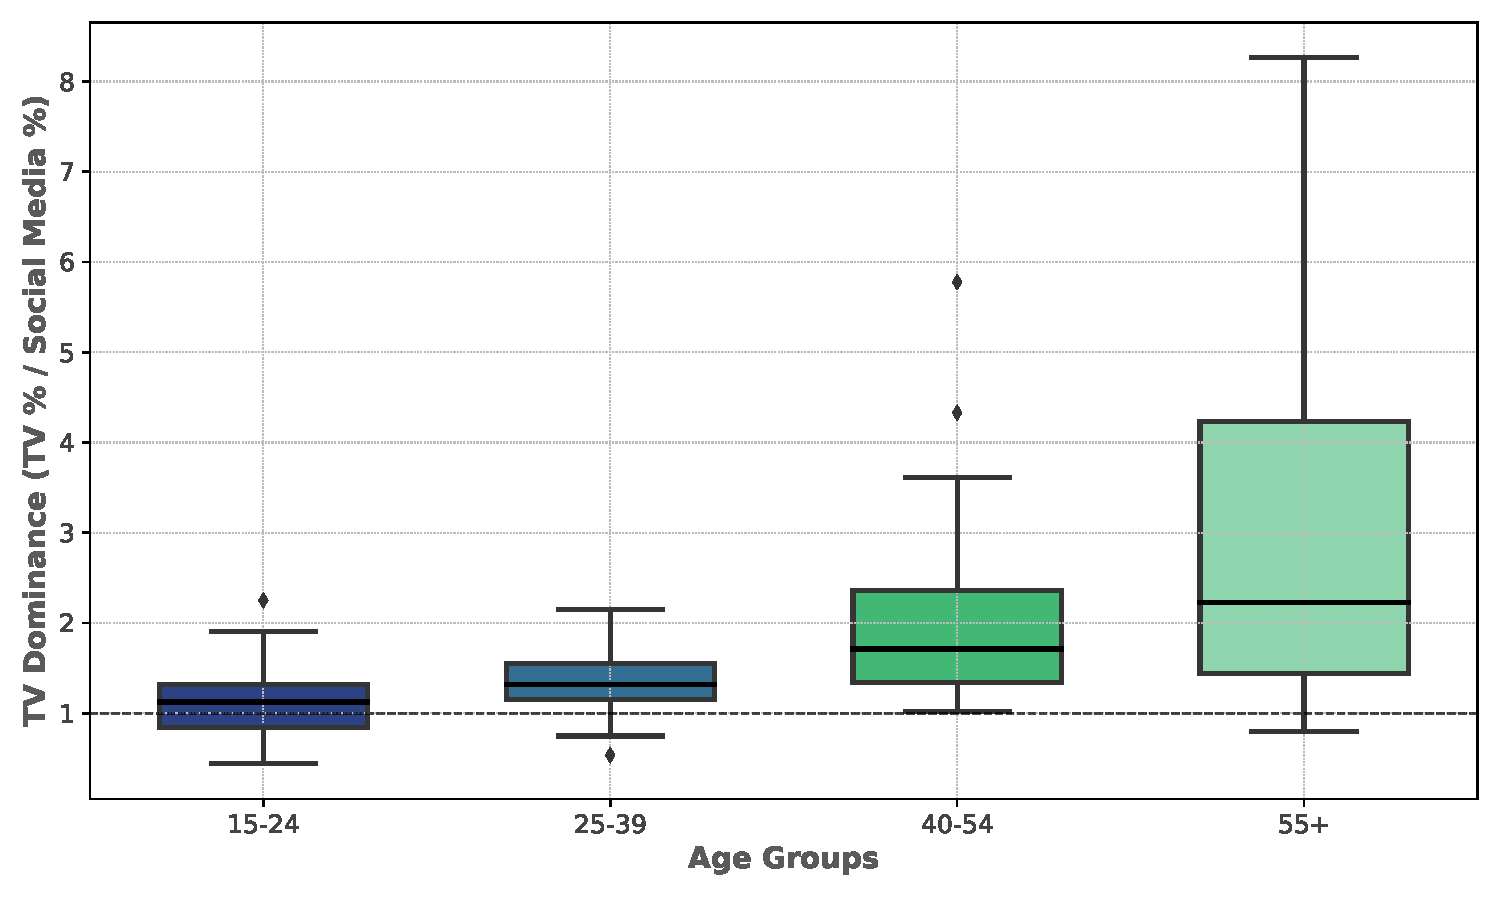
\includegraphics[width=130mm]{figures/age_cohorts_full}
		\caption*{\small \textit{Note:} Histogram of the preferred media used for political information in Europe. Using data for the 27 countries in Eurobarometer survey under the question \textit{"What media have you used the most to access news in the past 7 days?" }. $N=112059.$ 
			Source: Eurobarometer, 2022. }
		\label{fig:motivation2}
	\end{figure}
	
	
	

	
	
Similarly, traditional media still enjoy higher credibility than digital-only outlets or news encountered on social platforms. Nearly half  of survey participants (49 \%) say they trust public TV and radio—well above printed newspapers (39 \%) or news found on social networks and messaging apps (each below 15 \%) \citep{eurobarometer2022}. This credibility premium is closely linked to rising concern about fake news: respondents who worry most about disinformation are also the likeliest to turn to traditional broadcasters when verifying what is true. In the era of AI-enabled misinformation, audiences therefore continue to see traditional outlets—especially prime-time newscasts—as the primary source of political information, highlighting the importance of analyzing these markets. 
	
%	https://www.europarl.europa.eu/news/es/press-room/20220704IPR34401/eurobarometro-los-europeos-confian-mas-en-los-medios-informativos-tradicionales
	
	
	
	
	
	\subsection{Spanish Politics and TV News}
	
	
	
Here, I provide context on the Spanish political party system around my electoral period. I then describe the main TV channels of my analysis both in terms of their audience size and  the political composition of their audiences. 

	
	
	
	\subsubsection*{Spanish Political Context}
	

	

	
	
	Political power in Spain has historically been dominated by a two-party system, with government alternating between the Socialist Party (PSOE) and the People’s Party (PP). During my sample period (December 2022–July 2023), Spain was governed by a PSOE-led coalition under President Pedro Sánchez, first in alliance with Unidas Podemos (UP) and, after its relaunch, SUMAR,  with the main opposition led by PP and the extreme-right party VOX.\footnote{Relevant for this period of study is the integration of Podemos into the new party SUMAR. All classification metrics account for this transition, but throughout the text I refer to UP as either Podemos or SUMAR after its creation.} Although regional and independentist parties play a major role in the political environment, they are excluded from this analysis. For the remainder of the paper, parties are pooled into two blocs—right (PP and VOX) and left (PSOE and UP).
	
	
	 The extreme-right party VOX made notable gains in the May 28, 2023 regional elections, fueling speculation of a PP–VOX coalition. In response to these results, the day after the regional elections, President Sánchez decided to bring forward the general elections to July 23, 2023. In that election, the PP became the largest parliamentary group, though without the possibility of forming an absolute majority, which led  the left coalition to maintain power. 
	
	
	
	
	
	
	
	
	
	
	\subsubsection*{Spanish TV News}
	
	
	The product analyzed in this paper is television news broadcasts. I focus on the four largest national channels: Televisión Española, the state‐owned public broadcaster; Antena 3 and La Sexta (Atresmedia group); and Telecinco (Mediaset). Altogether, their evening news editions capture around 50 \% of viewership—about 4.5 million viewers, or 10 \% of Spain’s population. By comparison, the most‐watched U.S. cable‐news program (Fox News) averages roughly 2.2 million  viewers. While these outlets drive the national news agenda, data limitations prevent inclusion of regional networks—most notably Catalonia’s TV3, which commands a substantial local audience and may exhibit distinct partisan dynamics. Future work can extend this framework to incorporate TV3 and other region‐specific channels.  
	


What is the political composition of these audiences? Figure \ref{fig:opinion} shows the correlation between individuals' preferred political party (left or right) and their preferred channel for acquiring political information under the question \textit{"What is your preferred TV channel for political content?"}. I condition only on \textit{partisan} individuals, i.e., those who report a preferred political party. Right-wing individuals  tend to watch Antena 3 (A3) more, whereas left-leaning individuals are divided between La Sexta and the public channel Televisión Española (TVE). Telecinco (T5)  appears in the middle, with weak correlations. This is consistent with the Mediaset group offering more entertainment oriented content as previously documented for Italy in \citet{durante_aer}.

	
	\begin{figure}[!htbp]
		\centering
		\caption{Correlation Between Preferred Channel and Political Party}
		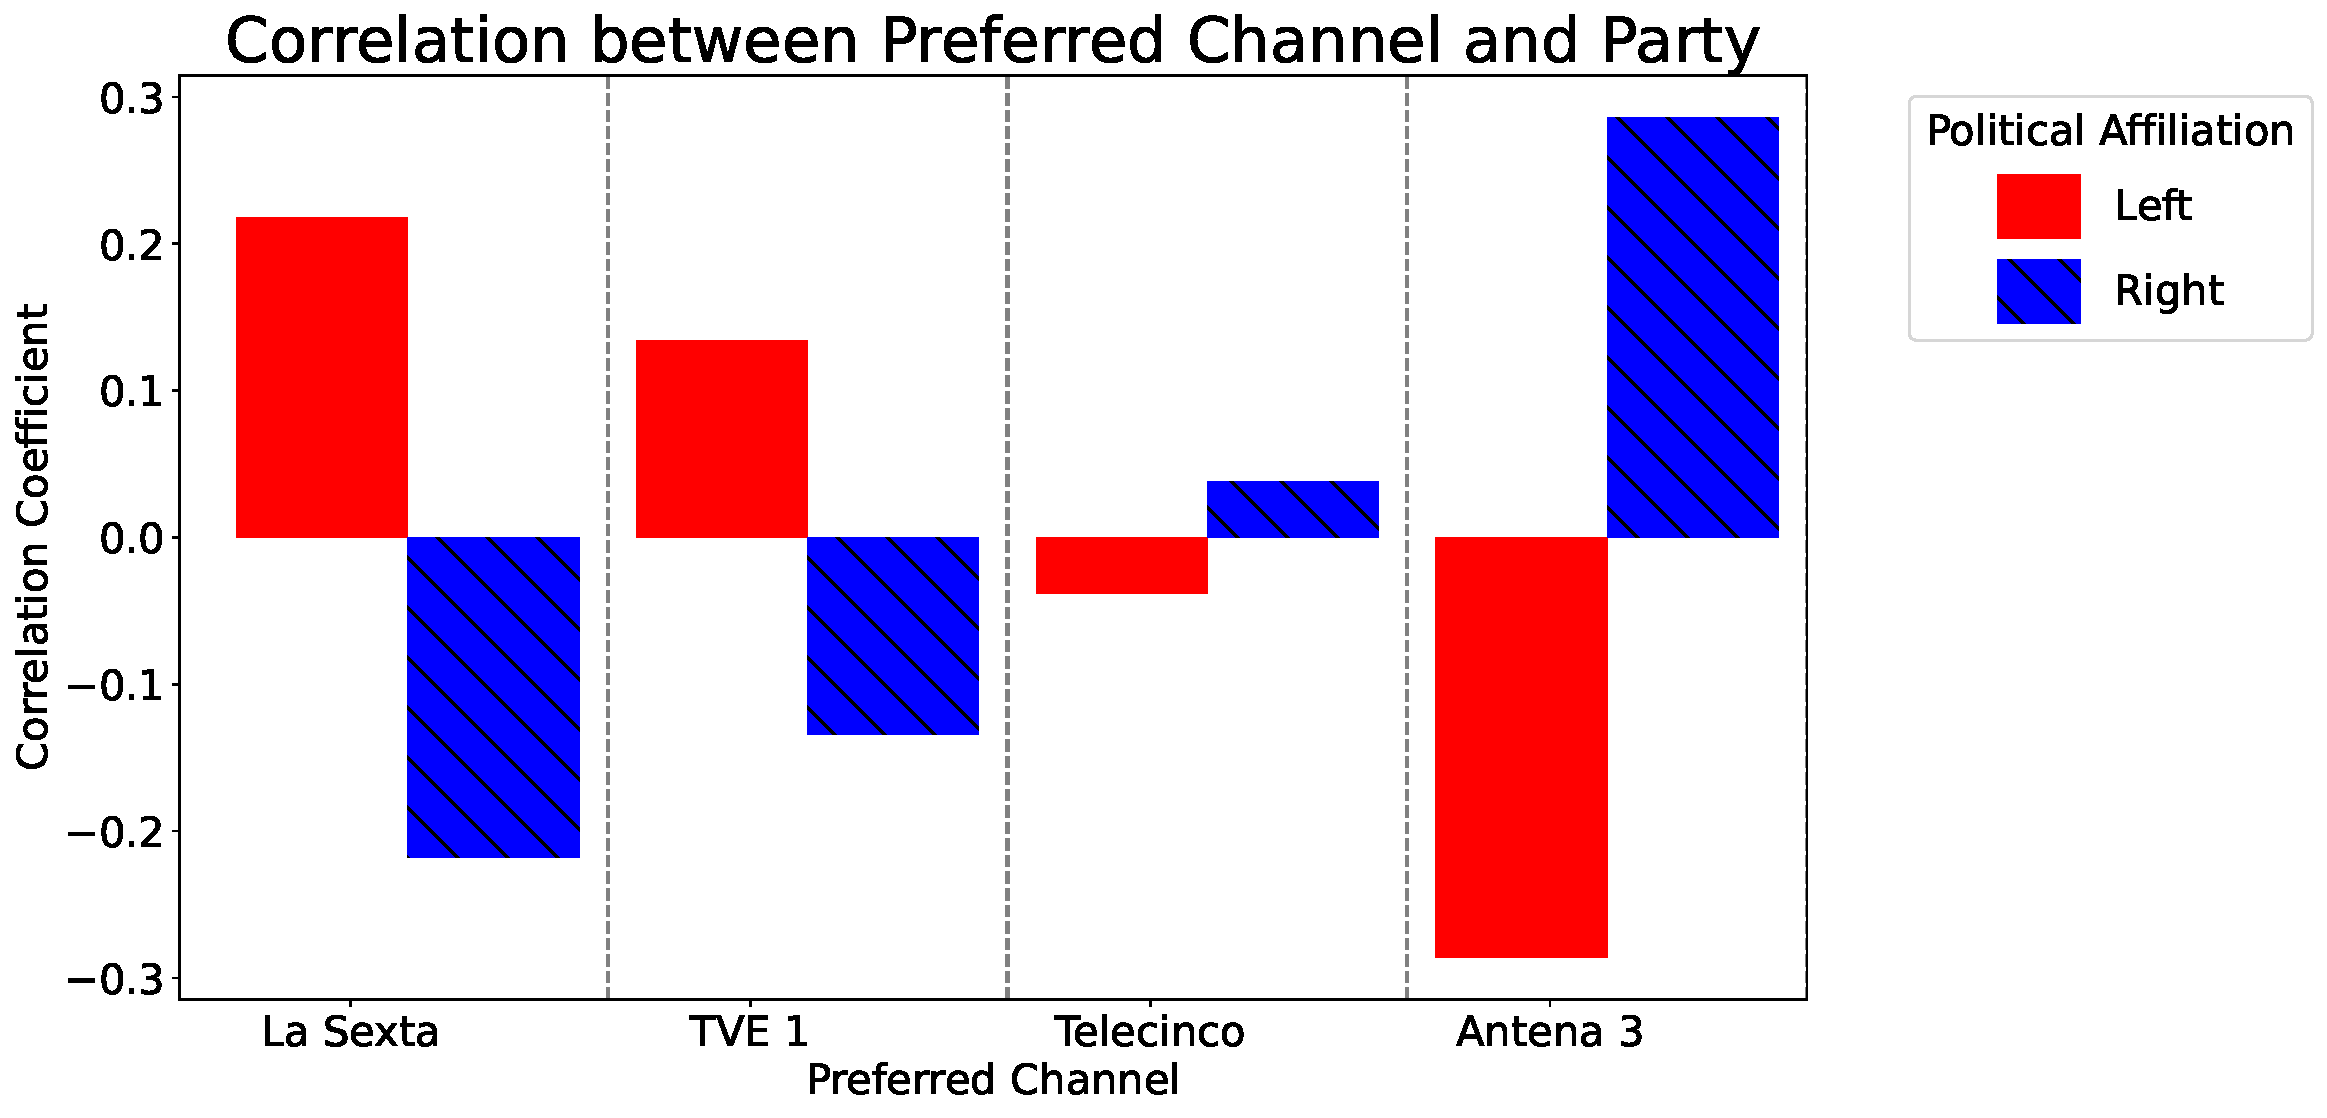
\includegraphics[width=120mm]{figures/corr_party_channel3}
		\caption*{\small \textit{Note:} Bars show correlation coefficients between individuals’ declared preferred political party (left or right) and their preferred TV news channel for political information. Respondents to the question are restricted to those that marked television as their main source of political information and those that report a preferred political party. Source: CIS, Encuesta Pre-electoral 2023.}
		\label{fig:opinion}
	\end{figure}
	
	

	
	
	
	To benchmark the degree of partisan sorting in television news against other media and prior studies, I compute the \emph{isolation index} \citep{gentzkow_isolation} for TV, radio, and the press. In a binary left–right setting, the index measures how much more likely a right-wing user is to encounter a co-partisan in the outlets that right-wing audiences visit than a left-wing user would in the outlets left-wing audiences visit. An isolation index of zero indicates no additional clustering by ideology (i.e., right- and left-leaning viewers consume the same outlets), while an index of one corresponds to complete segregation, where each group encounters only its own members.\footnote{The formal definition appears in Appendix  Section~\ref{sec:isolation}. Results of the isolation index and its decomposition by party bloc and can be seen in  Appendix Table~\ref{tab:isolation_table}. On television, right-leaning viewers face 41\% right exposure vs.\ 30\% for left-leaning viewers (11 pp). In the press: 43\% vs.\ 25\% (18 pp). On radio: 52\% vs.\ 24\% (29 pp).} Television is the least isolated medium (11 pp), followed by the press (18 pp) and radio (29 pp).
	

	
	
To contextualize these results, I compare them with the most recent estimates available for France  \citep{Dejean2022PartisanSE} and the U.S. \citep{gentzkow_isolation} (Table~\ref{tab:isolation_table_compare}). Spanish TV is about 8 p.p. more isolated than French TV and nearly 10 p.p. more than U.S.\ broadcast TV. This higher media segregation aligns with cross-country surveys that place Spain among the top most polarized electorates worldwide \citep{edelman_trust_2023}.
	
	
	
	
	
	%To contextualize these results, I compare them with the most recent estimates available for France in 2022 \citep{Dejean2022PartisanSE} and the U.S.\ in 2008 \citep{gentzkow_isolation} (Table~\ref{tab:isolation_table_compare}). Spain exhibits higher levels of partisan isolation across all media, consistent with the high levels of political polarization in the electorate \citep{edelman_trust_2023}.
	%Television in Spain is about 8 percentage points more isolated than  French TV and nearly 10 pp above U.S.\ broadcast TV.
	
	Taken together, the previous evidence reveals several facts. Television is the predominant and most trusted source to acquire political information in Europe. Additionally, the cross-country ranking reveals a common pattern: newspapers and radio are more ideologically segmented than broadcast TV, while Spain shows overall higher segregation. Since media effects are limited when audiences are already sorted, this pattern suggests greater potential for television to influence attitudes and less for radio or newspapers, where audiences are already politically aligned. This distinction is crucial when considering the external validity of my results for other media environments.
	
	
	

	
	
	\section{Data and Descriptive Evidence}
	\label{sec:data}

	I assemble a unique dataset that captures both the demand and supply sides of TV news. For the demand side, I have minute-by-minute viewership data for the four main channels that offer daily news programs: TVE, A3, La Sexta, and T5. On the content side, I build a scraping pipeline that records the daily news programs live and processes this information into text. This dataset spans from December 2022 to July 2023 on a daily basis. It is complemented by all the stories published in Spanish by the largest news provider. Finally, I make use of congress speeches, survey and weather data.
	
		\subsection{Data}
		
			\textbf{TV Content}
		
		I record daily  videos for both the midday and evening news editions. This leads to a total of 563 hours of content. I rely on Google Cloud infrastructure to store and process the data. Videos are converted to audio, and I use machine learning (\textit{speech-to-text}) to obtain text transcripts. Although visuals are not used in the main estimation due to computational constraints, I show comparisons between image and text metrics below. A summary of the entire downloading pipeline is provided in Appendix Section \ref{sec:appendix_models}.
		
		News programs offer a unique environment to test substitutability for several reasons. Even though channels offer other political programs, the homogeneity of these products allows for very clean comparisons. These programs are broadcast every day at almost the same time and all share a very similar structure, with a presenter introducing the main stories of the day. Their lengths are similar, with the shortest show (A3) averaging 32 minutes and the longest (TVE) 42 minutes.
		
		TV news programs are also highly fact-checked and they remain the most trusted source of information in Spain.\footnote{The Digital News Report 2023 reveals notable patterns in public trust towards news media across Europe, with Spain reflecting a stable but modest level of confidence. According to the report, the public service broadcaster RTVE and A3 Noticias continue to rank as the most trusted news sources, with trust levels of 48\% and 51\%, respectively. La Sexta registers  approximately 42\%, and T5 follows at 41\% \citep{reuters_dnr_2023}.} This fact is important as it ensures a cleaner interpretation of the audience choice data as revealed preferences for the content consumed and limits the extent of fake news as an additional dimension in the editorial strategy of the outlets. 
		
	
	\textbf{Audience Data}
	
	I use Audimeter, a high-frequency audience data source provided by Kantar Media. I observe the total amount of viewers for each channel  each day and minute. Variation over minutes will not be exploited. Instead, I rely on the initial audience at the beginning of the shows each day (i.e., minute-zero audience). For the model estimation, I compute the audience share variable  as the number of viewers divided by the potential number of TV-viewing households within a given region also provided by Kantar Media. 
	Although I do not have individual-level data on choices, I have geographical disaggregation for 15 autonomous regions in Spain (also referred to as regions hereinafter), which I match to survey demographics.\footnote{The Canary Islands and La Rioja are excluded due to different time zones and zero market shares, respectively. Similarly, peak days with sports events that altered the news schedule were also removed.} The shares are specific to the evening TV news shows, which, with the exception of La Sexta at 20:00, start at 21:00 daily. For this analysis, this channel’s program is treated as if it occurred simultaneously with the others.
	
	%\footnote{This might pose problems in the substitutions toward the outside option and specifically with  \textit{connected substitutes} assumption in \cite{berry2013connected}. Specifically, invertibility of demand requires weak substitutatbility across  }
	

	
	\textbf{Agencia EFE}
	
	I obtain all news stories published in Spanish by one of the largest news agencies in the world, Agencia EFE (or henceforth, EFE). I have information on the title of each story along with a short summary segment for  32,525 stories in my sample period.
	
	Similar to Reuters or Associated Press, this agency mainly sells content and images to third-party newscasts. All the outlets in my sample are clients of  EFE.\footnote{See collaborations with \href{https://www.telecinco.es/autores/agencia-efe/}{Mediaset}, \href{https://cadenaser.com/nacional/2024/09/22/el-teletexto-una-herramienta-olvidada-que-aun-perdura-en-nuestras-televisiones-cadena-ser/}{Atresmedia}, and \href{https://www.rtve.es/rtve/20130301/rtve-agencia-efe-firman-convenio-colaboracion/611440.shtml}{RTVE}.} 


	\textbf{Congress Speeches}

 I collect the complete set of plenary session transcripts from the Spanish Congress of Deputies during the XV Legislature. The official Diarios de Sesiones del Pleno are published in PDF format on the Congress website.\footnote{Available at: \url{https://www.congreso.es/es/busqueda-de-intervenciones}.} There are a total of $1411$ interventions. Each of them is linked to the corresponding speaker, and I match speakers to their parliamentary group using official records. This dataset is used for robustness of the text classification. 

	
	\textbf{Survey Data}
	
	To understand polarization behavior, I use survey data gathered from the Centro de Investigaciones Sociológicas (CIS). Specifically, I rely on the "intention to vote" question and map it onto my binary left–right spectrum according to the parties described above. These data are monthly and are in cross-sectional format.
	
	\textbf{Weather}
	
	I use meteorological data on daily rainfall deviations per region for the time span matching the TV news programs (18:00–00:00) from the Spanish Meteorological Agency (AEMET).
	

	
	
	
	\subsection{Text Classification}
	
	As noted above,  news programs present a very similar structure in length, broadcast time, and format. This homogeneity allows for cleaner comparisons as opposed to general opinion shows, where characteristics differ starkly, but at the same time makes them almost perfect substitutes; the key differentiation (aside from vertical, quality components) being the way they treat the information. Here I describe how text analysis techniques can provide robust measures of political slant and effectively differentiate the outlets' treatment of  information. 
	

	
	\subsubsection*{Building Content Characteristics}
	
	Each day \(d\), channel \(j\) produces a set of stories \(S_{jd}\) indexed by \(s\). Empirically, these segments result from BERTopic clustering on the unstructured transcripts, which ensures that the LLM has enough context by feeding it the entire text of a given story. This leads to a total of 20,674 stories. The subset of political stories, \({P}_{jd}\subseteq S_{jd}\), is the set of all stories that mention national parties or prominent politicians in addition to general words related to politics, identified by keyword matches from Table~\ref{tab:politics}.
	
	Each \(s\in {P}_{jd}\) is fed into ChatGPT and  assigned a score: \({t}(s)\in\{-1,0,1\}\)\footnote{More details about the prompt and classification results can be found in Appendix Section \ref{sec:appendix_models}.} with ${t}(s)=1$ (${t}(s)=-1$) denoting a positive (negative) tone. Stories with a stance (i.e., \({t}(s)\in\{-1,1\}\)) also receive a party label \({p}(s)\in\{L(eft),R(ight)\}\), whereas neutral stories do not. 
	
	Notice that the broad classification of what is \emph{political} allows for stories without explicit mentions of  political actors to be classified as partisan. Table~\ref{tab:international} contains text examples of this.  Positive Left stories include, for instance,  an economic forecast from the European Commission and the opening of a new gigafactory, while Negative Left stories include court officers barricading courthouses for pay raises and fuel-price surges driven by the Ukraine war. These cases show how the classifier infers slant from thematic framing alone, assigning a political slant to national parties without explicit references to them. 
	
	
	Additionally, a story can be mapped to its length in minutes, \( \ell(s)\), with total length of the news programs  denoted by $L_{jd}$. I then define: 
	
	
	


		\begin{equation}\label{eq:controls}
		\begin{aligned}
			x_{jd}^{party+}&= \frac{1}{L_{jd}} \sum_{s \in P_{jd}}\bigg(\mathds{1}\{t(s)=1\} \times \mathds{1}\{p(s)=party\}\times \ell(s) \bigg) &\forall party \in \{L,R\} \\
			x_{jd}^{party-}&= \frac{1}{L_{jd}} \sum_{s \in P_{jd}}\bigg( \mathds{1}\{t(s)=-1\} \times \mathds{1}\{p(s)=party\} \times \ell(s)\bigg) &\forall party \in \{L,R\} \\
			x_{jd}^{political}&=\frac{1}{L_{jd}} \sum_{s \in P_{jd}}\ell(s).
		\end{aligned}
	\end{equation} 
	

 Combining all these characteristics—i.e., party label, tone, and minutes— Equation \eqref{eq:controls} represents the  shares of positive and negative minutes, as well as the share of airtime devoted to politics.	Similarly, I proxy the daily news landscape with all stories published in Spanish by the newswire agency EFE—$N\approx32.5K$ items over the sample. Mirroring the content covariates in~\eqref{eq:controls}, I classify every  story with the same pipeline and construct daily measures of the political mix in the set of stories available as:
	
	\begin{equation}\label{eq:efe}
		\begin{aligned}
			z_d^{\,party+} &= \frac{1}{|\mathcal{N}_d|}\sum_{s\in \mathcal{P}_d}
			\bigg(\mathds{1}\{t(s)=1\}\times \mathds{1}\{p(s)=\textit{party}\}\bigg)
			&\forall\,\textit{party}\in\{L,R\},\\
			z_d^{\,party-} &= \frac{1}{|\mathcal{N}_d|}\sum_{s\in \mathcal{P}_d}
			\bigg(\mathds{1}\{t(s)=-1\}\times \mathds{1}\{p(s)=\textit{party}\}\bigg)
			&\forall\,\textit{party}\in\{L,R\},\\
			z_d^{\,\text{political}} &= \frac{|\mathcal{P}_d|}{|\mathcal{N}_d|},
		\end{aligned}
	\end{equation}
	
	where now \(\mathcal{N}_d\) denotes the total number of   stories on day~\(d\), and \(\mathcal{P}_d\) the subset of them classified as political under the same criteria as before. These variables will constitute the main controls and instruments for the empirical application in the next section. 
	

		\subsubsection*{Results of the Slant Classification}
	
	
	
	Figure \ref{fig:chat} plots each channel’s net average tone toward left‐ and right‐wing parties, calculated as the difference between positive and negative coverage from Equation \eqref{eq:controls} over the entire sample period.\footnote{Specific examples of stories with their tone classification can be seen in Appendix Table \ref{tab:examples_stories}.} Positive (negative) values indicate a net (un)favorable tone toward a party by that outlet. 
	
		\begin{figure}[!htbp]
		\caption{Average Tone Across Channels and Parties}
		\centering
		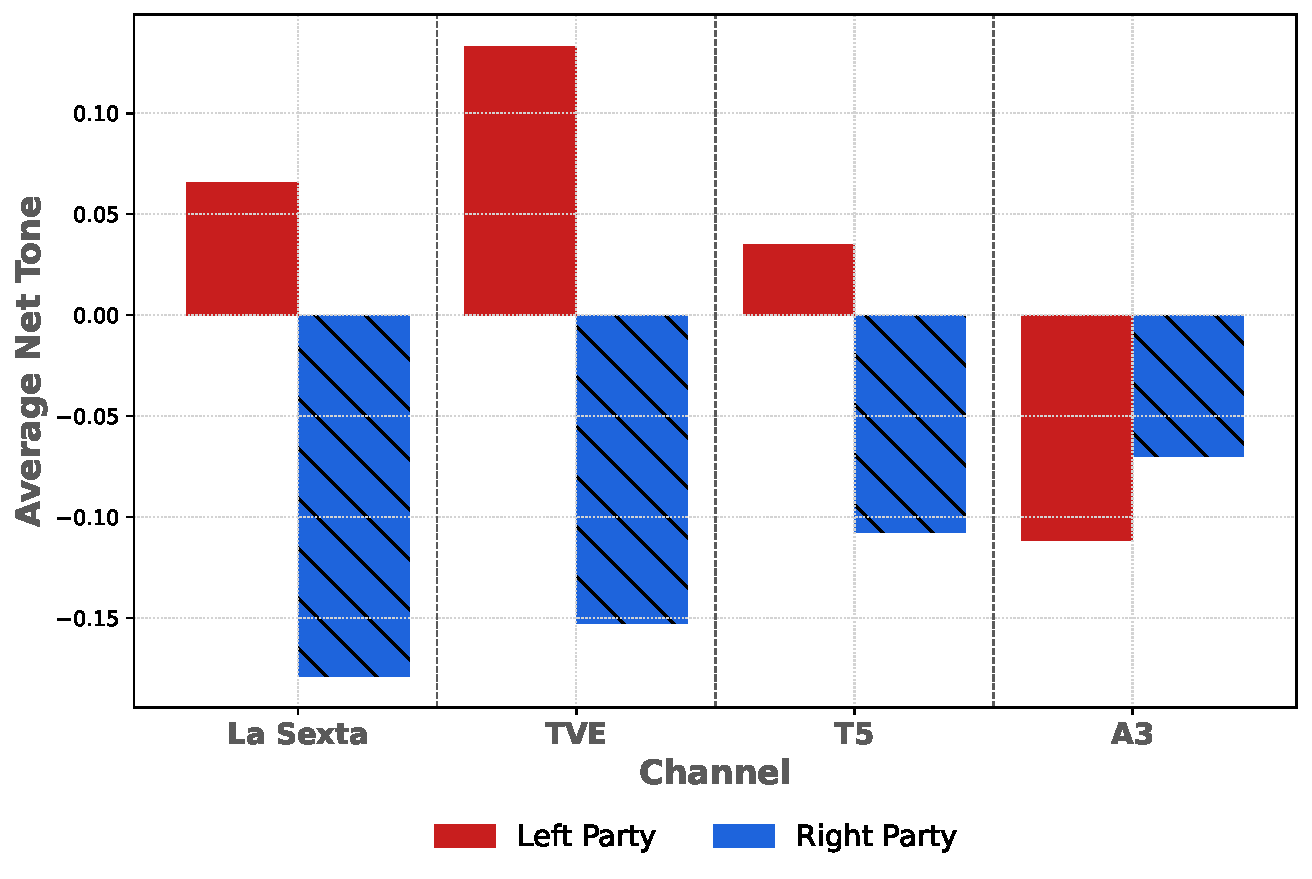
\includegraphics[width=120mm]{figures/chatgpt}
		\caption*{\small \textit{Note:} Bars show the average net tone toward left- and right-wing parties for each TV channel, computed as the difference between positive and negative minutes of coverage ( $	\bar{x}_j^{party+}-\bar{x}_j^{party-}$) as defined in Eq. \eqref{eq:controls}. Positive (negative) values indicate a net (un)favorable tone toward a party by that outlet.}
		\label{fig:chat}
	\end{figure}
	
	La Sexta and TVE tilt strongly pro-left, T5 sits near the center with a mild leftward bias, and A3 is the only channel  with a slight pro-right balance. Every channel exhibits a net negative tone toward the right-wing bloc, reflecting the fact that the left coalition held office throughout my sample period. As can be seen in some of the text examples in Tables \ref{tab:examples_stories} and \ref{tab:international}, the classifier interprets the passage of new laws or institutional visits as something positive for the incumbent. In practice, this meant an abundance of positive policy stories on the left and comparatively few favorable stories on the opposition, which pushes the average right-wing tone to be negative.
	
	
	
	
	%To compare these supply‐side slant scores with audience ideology (demand), I assign each channel an \textit{slant index} calculated as 
	
	
	To validate these results, I compare outlets' slant classification with the ideological composition of their channels that comes from survey data. 	I assign each channel a \textit{slant index} calculated as 
	
	
	
	\begin{equation}\label{eq:ideo_index}
		\begin{aligned}
			& Slant_j \equiv \bigl(\bar{x}_j^{R+}-\bar{x}_j^{R-}\bigr)-\bigl(\bar{x}_j^{L+}-\bar{x}_j^{L-}\bigr).
		\end{aligned}
	\end{equation} 


% Here, slant refers to the party balance of each channel both in terms of their tone and proportion of time spent on each party. More positive values indicate coverage more favorable to right parties relative to left,  and negative values the reverse. This formulation allows to collapse party positions into a single dimension. To asses whether the slant that comes from the text classification is consistent, I compare it with outlet's predicted left-right positions that come from survey data on the ideology of their viewers (i.e those shown in Figure \ref{fig:opinion}). Under a demand driven equilibrium, we would expect both to be similar. I thus derive the position of each outlet according to their viewers preferences  by using the same slant formula on the correlations between preferred political party and most consumed outlet.  I then normalize both metrics so that the most extreme channels take values of $-1$ and $1$. This enables comparisons across the two different measures.
 
 Here, slant refers to the party balance of each channel both in terms of their tone and proportion of time spent on each party. More positive values indicate coverage more favorable to right parties relative to left,  and negative values the reverse. This formulation allows to collapse party positions into a single dimension.  To assess whether the text-based slant is consistent, I compare it with each outlet’s predicted left–right position derived from survey data on viewers’ ideology described in the previous section (Figure \ref{fig:opinion}). Under a demand-driven equilibrium, we expect the content offered to match viewers' political orientation. 
 

 
 Figure~\ref{fig:channel_ideology_lines} displays the normalized scores: panel~(a) shows outlets' positions based on viewers’ ideology, and panel~(b) based on their text‐based slant. The consistent left‐to‐right ranking and the close score values in both panels confirms that the LLM‐based classification is similar to  the distribution of audience preferences. Below, I also show robustness of the text classification and comparisons with other methodologies previously used in the literature.
		
	
	
		\begin{figure}[!htbp]
		\centering
		\caption{Normalized Slant Index by Channel}

		% Panel (a): ChatGPT-based
		\begin{minipage}[t]{0.49\textwidth}
			\centering
					(a) Demand: Viewers' ideology
		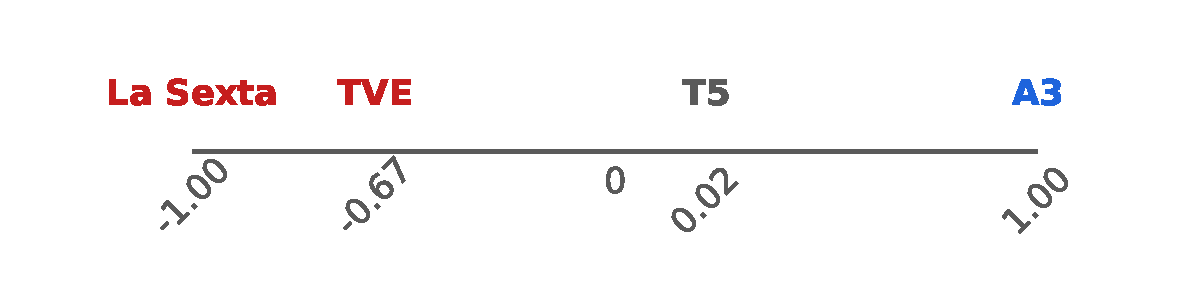
\includegraphics[width=\linewidth]{figures/congress_line_cis}
		\end{minipage}
		\hfill
		% Panel (b): CIS-based
		\begin{minipage}[t]{0.49\textwidth}
			\centering

			
				(b) Supply: Text classification
			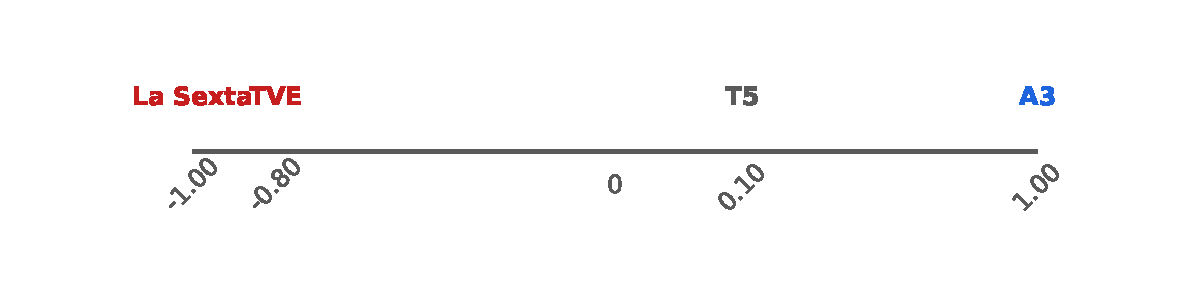
\includegraphics[width=\linewidth]{figures/congress_line_chatgpt}
			
			
		\end{minipage}
		
		
		\caption*{\small \textit{Note:} The figure compares normalized left–right positions for the outlets in the sample. Panel (a) uses viewer ideology data from CIS survey data, using the difference in correlation coefficients between right and left; panel (b) uses GPT-based slant index as described in Equation \eqref{eq:ideo_index}. Values are normalized so that the two most extreme channels take values -1 and 1 to enable comparisons across the two different metrics. }
		\label{fig:channel_ideology_lines}
	\end{figure}
	
	\FloatBarrier
	
	\paragraph{Robustness of the text classification.}
	
	The use of LLMs as classifiers has gained popularity for the classification of political stances, with even higher accuracy scores for ideological classification compared to human annotators \citep[see, e.g.,][]{lemens,tornberg2023,Gilardi2023ChatGPTOC}. However, two main concerns arise. First, LLMs have been shown to suffer from prompt instability, producing inconsistent results across multiple runs of the same query. Second, one may question the performance of alternative text classification methods. In Appendix Section~\ref{sec:robustness}, I address these concerns. I first demonstrate that the classification remains stable under repeated queries. Second, I compare my results with previous methods used to assess slant. Specifically, methods based on similarity to congressional speeches \citep{gentzkow2010media,laver2003extracting} yield a consistent ideological ranking of the outlets although the spread of the ideological spectrum differs. I also apply face recognition to compare the slant measure with the standard metric based on politicians’ airtime. This metric, widely used by regulatory agencies and in prior research, produces a completely different scenario, in which all channels appear more homogeneous, and it fails to predict actual slant.
	
	Taken together, these results show the robustness of LLMs for slant classification and indicates the limitations of traditional measures—such as image-based metrics—to assess plurality. 
	
	
	

	\subsection{Descriptive Evidence}


	\subsubsection*{TV News Consumption and the Election Campaign}

	
	
	
	I divide the sample into two periods. The \textit{off-campaign} period runs from the start of data collection (December 2022) to May 13, 2023, the date of the first publicly announced campaign for the regional elections. The \textit{campaign} period covers both the regional and general election campaigns and ends on July 23, 2023 (general election day). 
	
	
The campaign period coincided with the summer months, in which seasonality drives audience numbers down. However, salient political events typically retain attention. To see the impact of these two effects, 	Figure \ref{fig:audience_share} shows the time series evolution of the audience shares for each of the four channels in my sample. All outlets nearly maintain their share during the campaign: A3 moves from 17.2\% to 16.9\%, T5 from 9.4\% to 10.1\%, La Sexta from 5.6\% to 6.0\%, and TVE from 10.2\% to 10.3\%. 
	
	
		\begin{figure}[!htbp]
		\caption{TV Audience over Time}
		\centering
		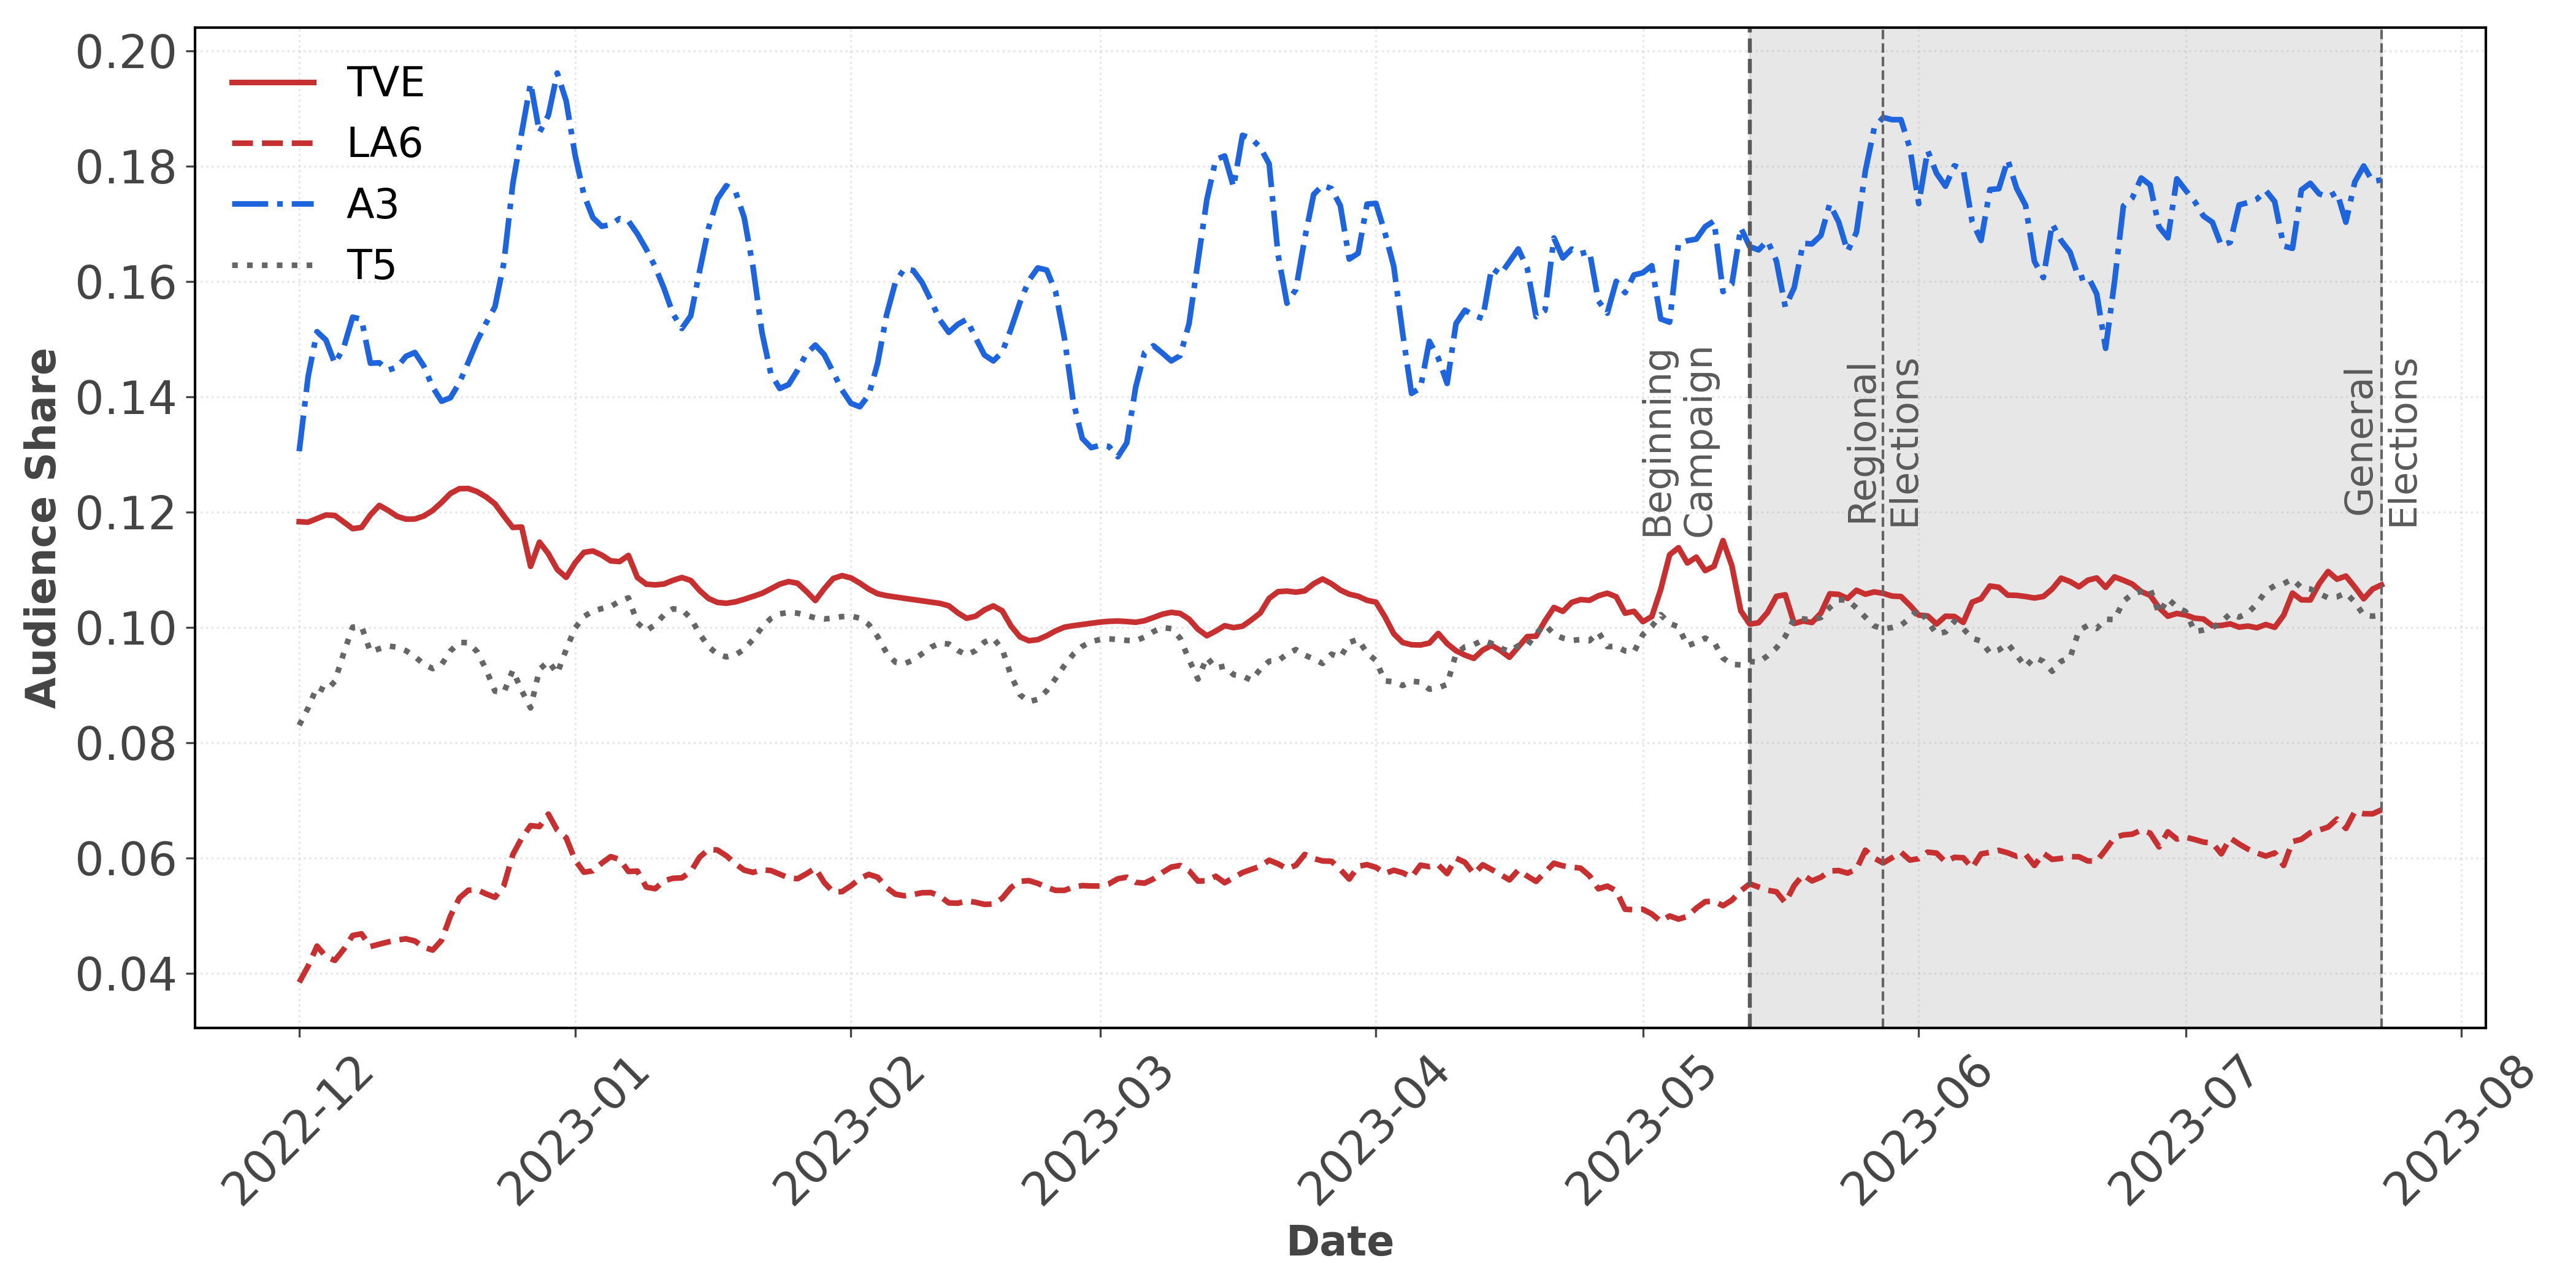
\includegraphics[width=150mm]{figures/tv_audience_sharev2}
		\caption*{\small \textit{Note:} The figure represents the share of audience for the TV outlets in my sample.  Vertical, dashed lines indicate the date of the beginning of the campaign, the regional and the general elections, respectively. The shaded area represents the \textit{campaign} period considered.  All series are smoothed using a centered rolling mean with a 9-day window to reduce noise and highlight underlying trends over time.}
		\label{fig:audience_share}
	\end{figure}
	
	

This stability of the audience share numbers contrasts with the evolution in the total viewership. All channels lose audience levels in this period—on the order of 15–25\%—with A3 still the largest (roughly 2.2M viewers off-campaign vs. 1.7M during the campaign) and the remaining channels experience similar proportional declines (see Figure  \ref{fig:audience_total}). This  suggests that information seeking  helps outlets maintain their slice of attention even as overall viewing falls in summer months. 


	
		\subsubsection*{Political Coverage and the Election Campaign}
		
		
	
	
Election campaigns concentrate public attention on politics and shift newsroom priorities. Consistent with this, Figure \ref{fig:coverage} shows that the share of political content rises sharply for both television and the EFE newswire. On average, TV channels devote 18\% of airtime to politics off-campaign, rising to 30\% during the campaign. For EFE, the share of political stories increases from 43\% to 51\%. Both series display similar seasonality (Pearson correlation  $r=0.59$), dipping in non-political periods such as Christmas and Easter.\footnote{	There is, however, heterogeneity in how closely outlets follow the agency in terms of political coverage. A3 exhibits the strongest co-movement with EFE in political coverage ($r=0.67$), followed by T5 ($r=0.48$), TVE ($r=0.38$), and La Sexta ($r=0.26$). Figure \ref{fig:political_by_channel} in the Appendix shows the time series decomposition of political coverage by outlet.}
	

	
	
		
	\begin{figure}[!htb]
		\caption{Proportion of Political Coverage over Time}
		\centering
%		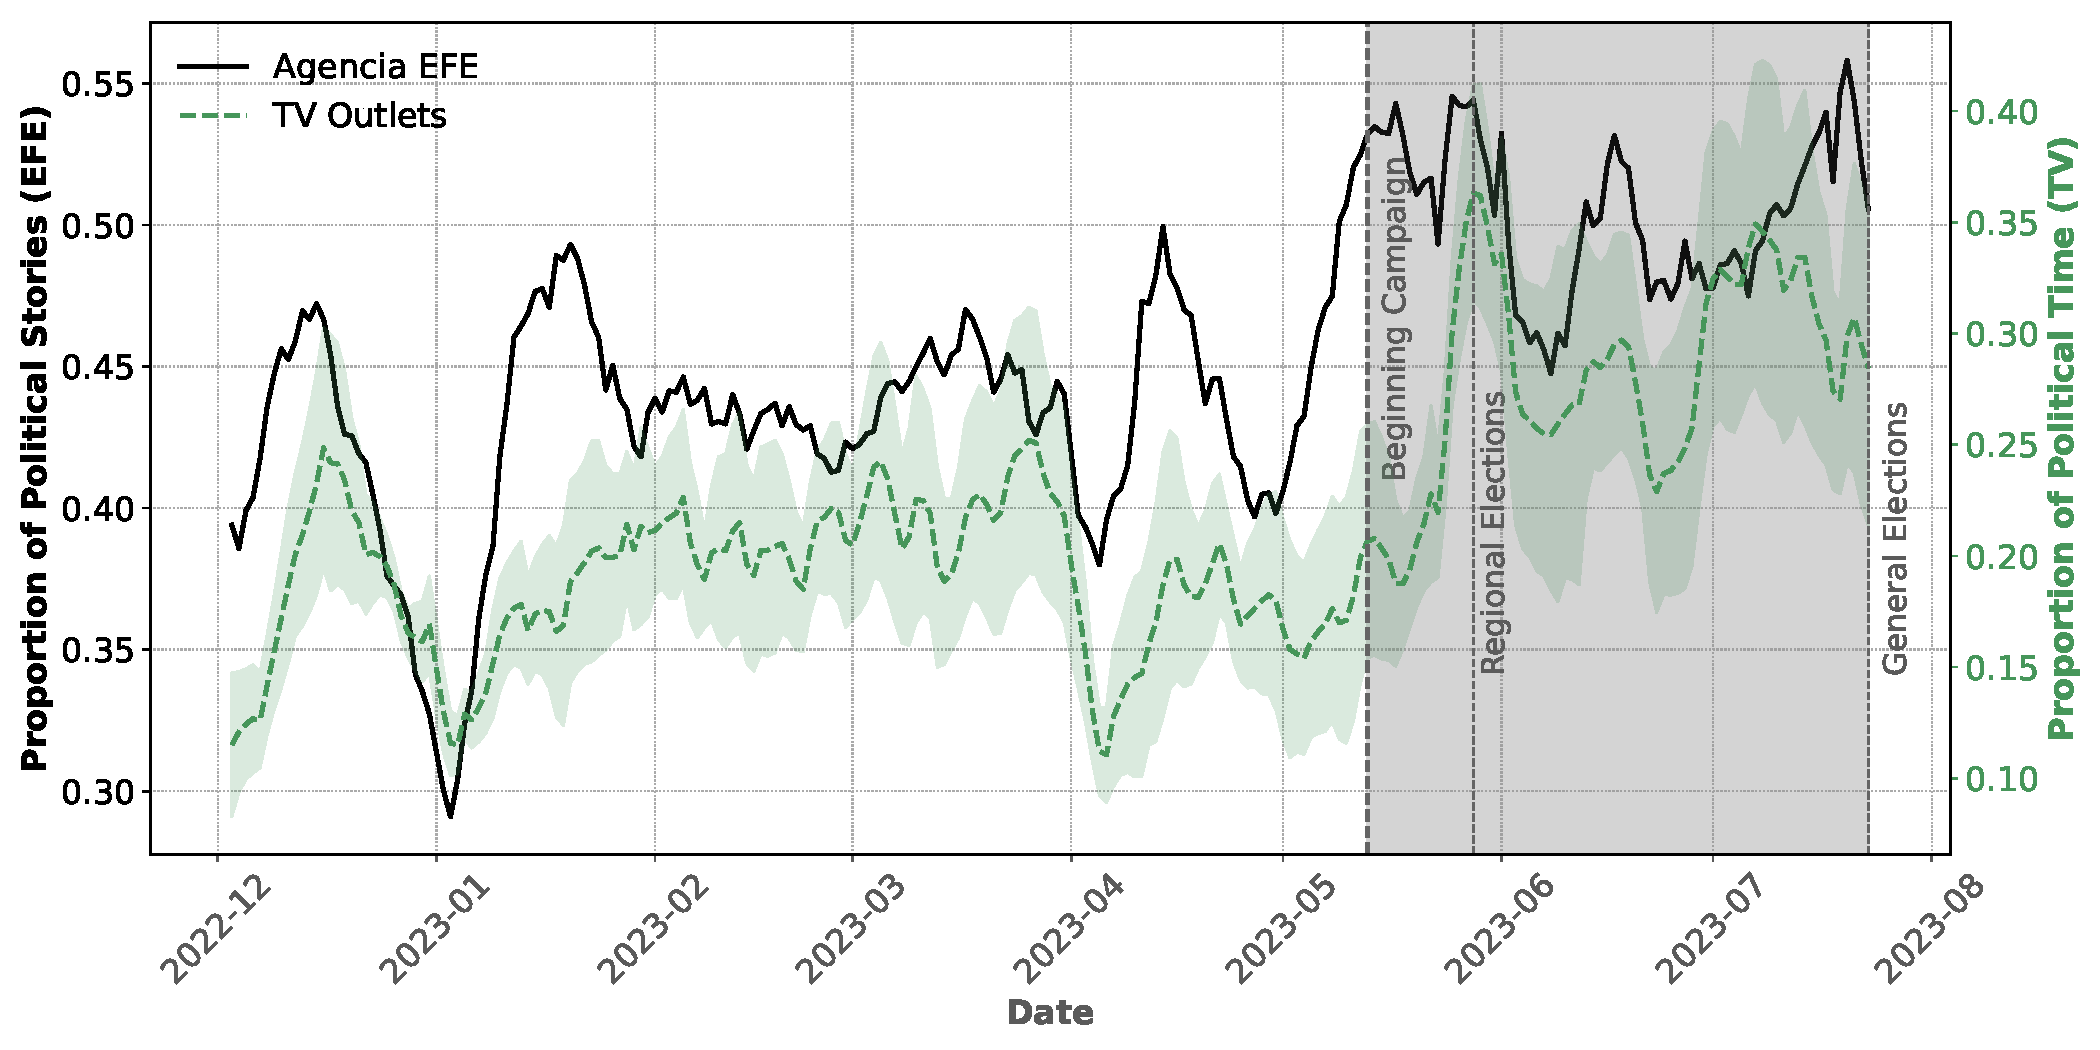
\includegraphics[width=150mm]{figures/political_words_bothv2}
				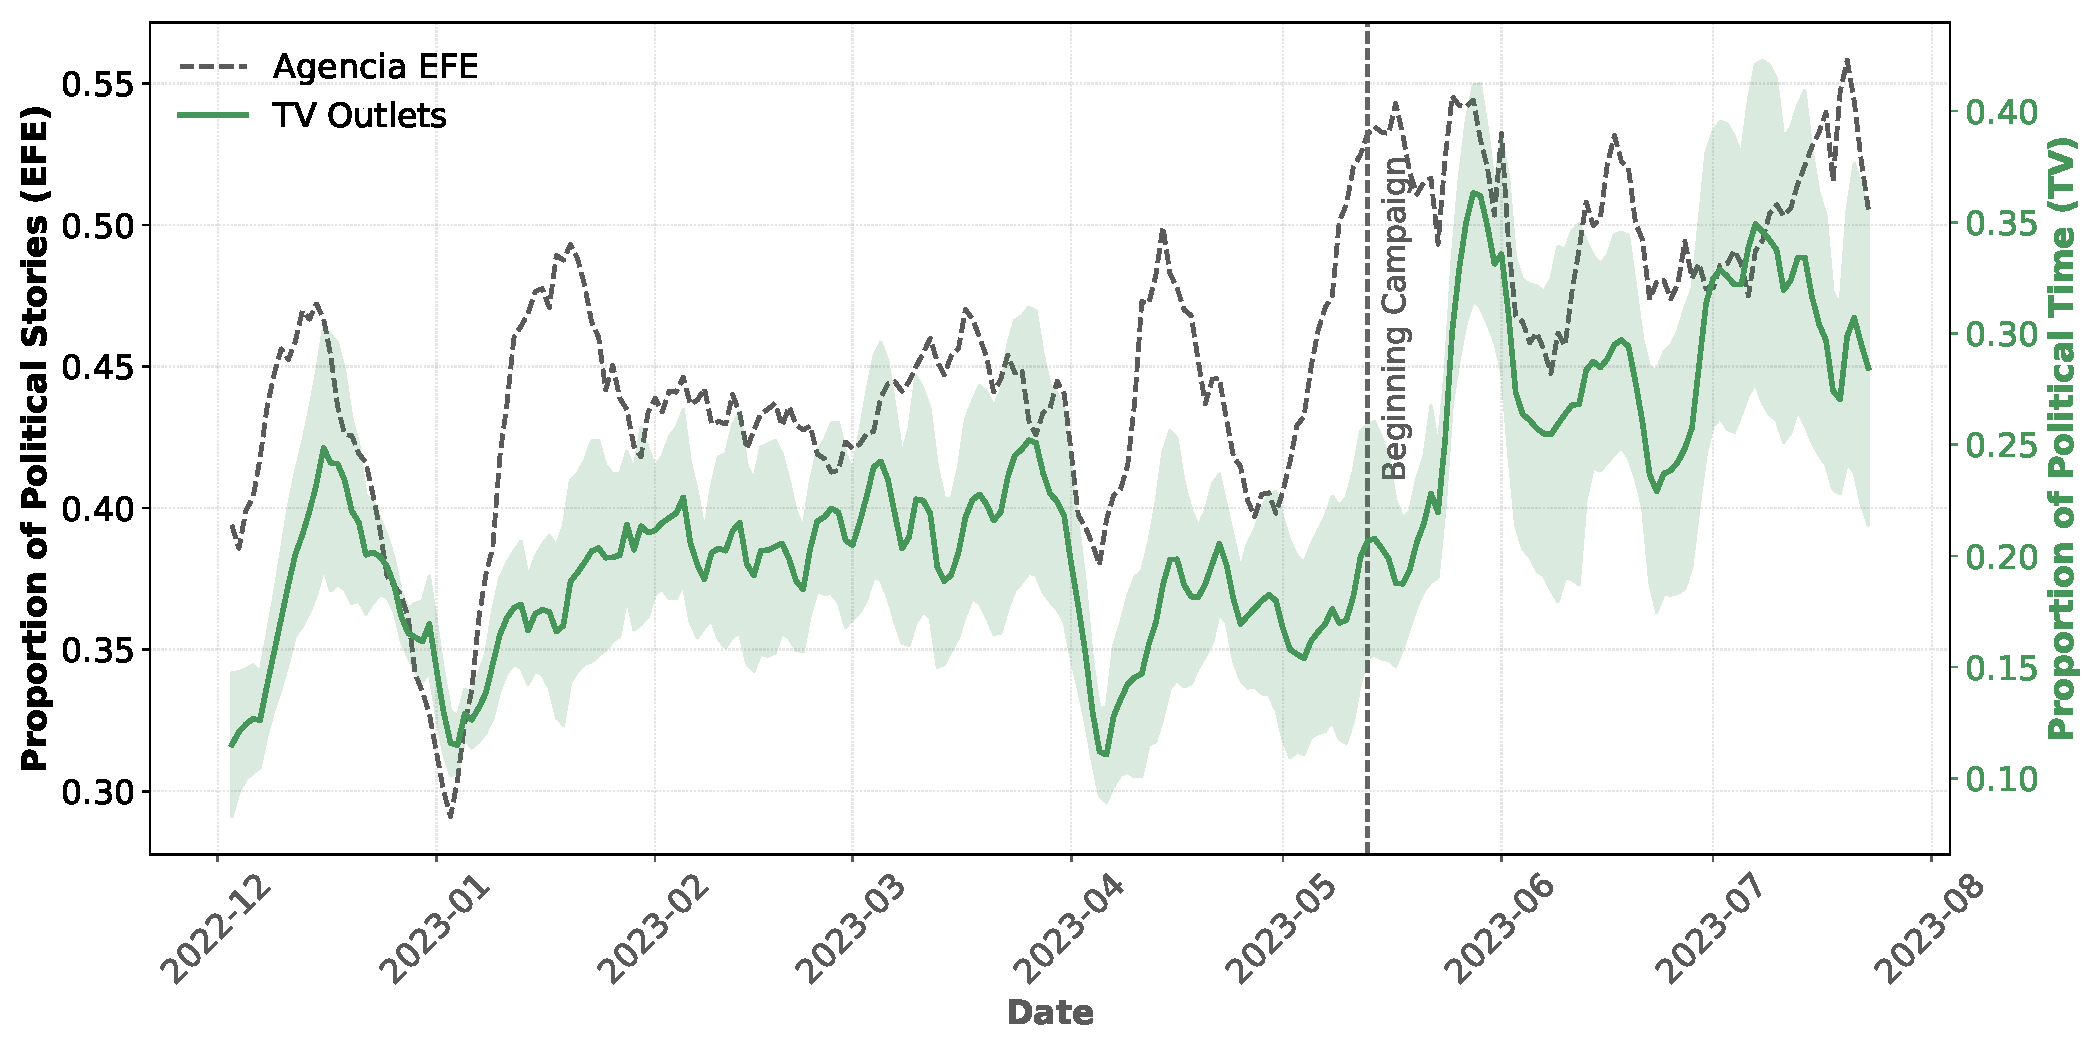
\includegraphics[width=150mm]{figures/political_words_both}
		\caption*{\small \textit{Note:} The figure represents the proportion of political content for the TV outlets (dashed) and  EFE (solid) as defined in Eqs. \eqref{eq:controls} and \eqref{eq:efe}, respectively. All series are smoothed using a centered rolling mean with a 9-day window.}
		\label{fig:coverage}
	\end{figure}
	

	
	

	
	\begin{comment}
		\begin{tabular}{lcc}
			\toprule
			\textbf{Outlet} & \textbf{Pre-campaign} & \textbf{During campaign} \\
			\midrule
			A3 & 0.263 & 0.399 \\
			TVE & 0.126 & 0.179 \\
			LA6 & 0.173 & 0.252 \\
			T5 & 0.136 & 0.237 \\
			\addlinespace
			EFE (Factiva) & 0.432 & 0.508 \\
			\bottomrule
		\end{tabular}
	\end{comment}
 
	

	
\begin{comment}
	content...

\begin{table}[!htbp]
	\centering
	\caption{Proportion of Political Content}
	\begin{tabular}{lcc}
		\toprule
		\textbf{Outlet} & \textbf{Pre-campaign} & \textbf{During campaign} \\
		\midrule
		La Sexta & 0.173 & 0.252 \\
				TVE & 0.126 & 0.179 \\
		T5 & 0.136 & 0.237 \\
				A3 & 0.263 & 0.399 \\
		\addlinespace
		\hline
		Agencia EFE & 0.247 & 0.316 \\
		\bottomrule
	\end{tabular}
\caption*{\small \textit{Note:} The table shows the proportion of political content for the four TV channels, calculated as the proportion of time spent in politics; and for the Agencia EFE, calculated as the proportion of stories that are political. }
\label{tab:tests}
\end{table}
\end{comment}
	
		\FloatBarrier
	

%\subsubsection*{Political Slant and the Election Campaign}


Campaigns shift attention toward politics; the next natural question to ask then is which party benefits from this.   Figure \ref{fig:net_tone} shows the  evolution of slant index defined in Eq.~\eqref{eq:ideo_index}  for the newswire agency EFE and  the TV outlets.\footnote{Time series for all the individual outlets are shown in Appendix Figure \ref{fig:net_tone_by_channel}.} Positive (negative) values indicate coverage more favorable to the right (left).  EFE’s series is predominantly negative, indicating a systematic tilt toward the left on average. As noted earlier, this pattern largely stems from the governing left-bloc coalition, which, by holding power, receives greater visibility through coverage of official meetings, legislation, and related activities.


%Outlets co-move with the wire but in a less systematic way than the political coverage shown before. 
%The right-leaning A3 shows the strongest co-movement with EFE ($r=0.36$); the left-leaning channels TVE and La Sexta follow ($r=0.32$ and $r=0.24$, respectively), while T5,  exhibits a very small correlation ($r=0.02$). This last low value contrasts with the strong correlation shown for overall political coverage by T5. Figure highlights how the outlet presents a smoothed version of the newswire ideology especially before the campaign begins. 


\begin{figure}[!htb]
	\caption{Evolution of the Slant Index}
	\centering
	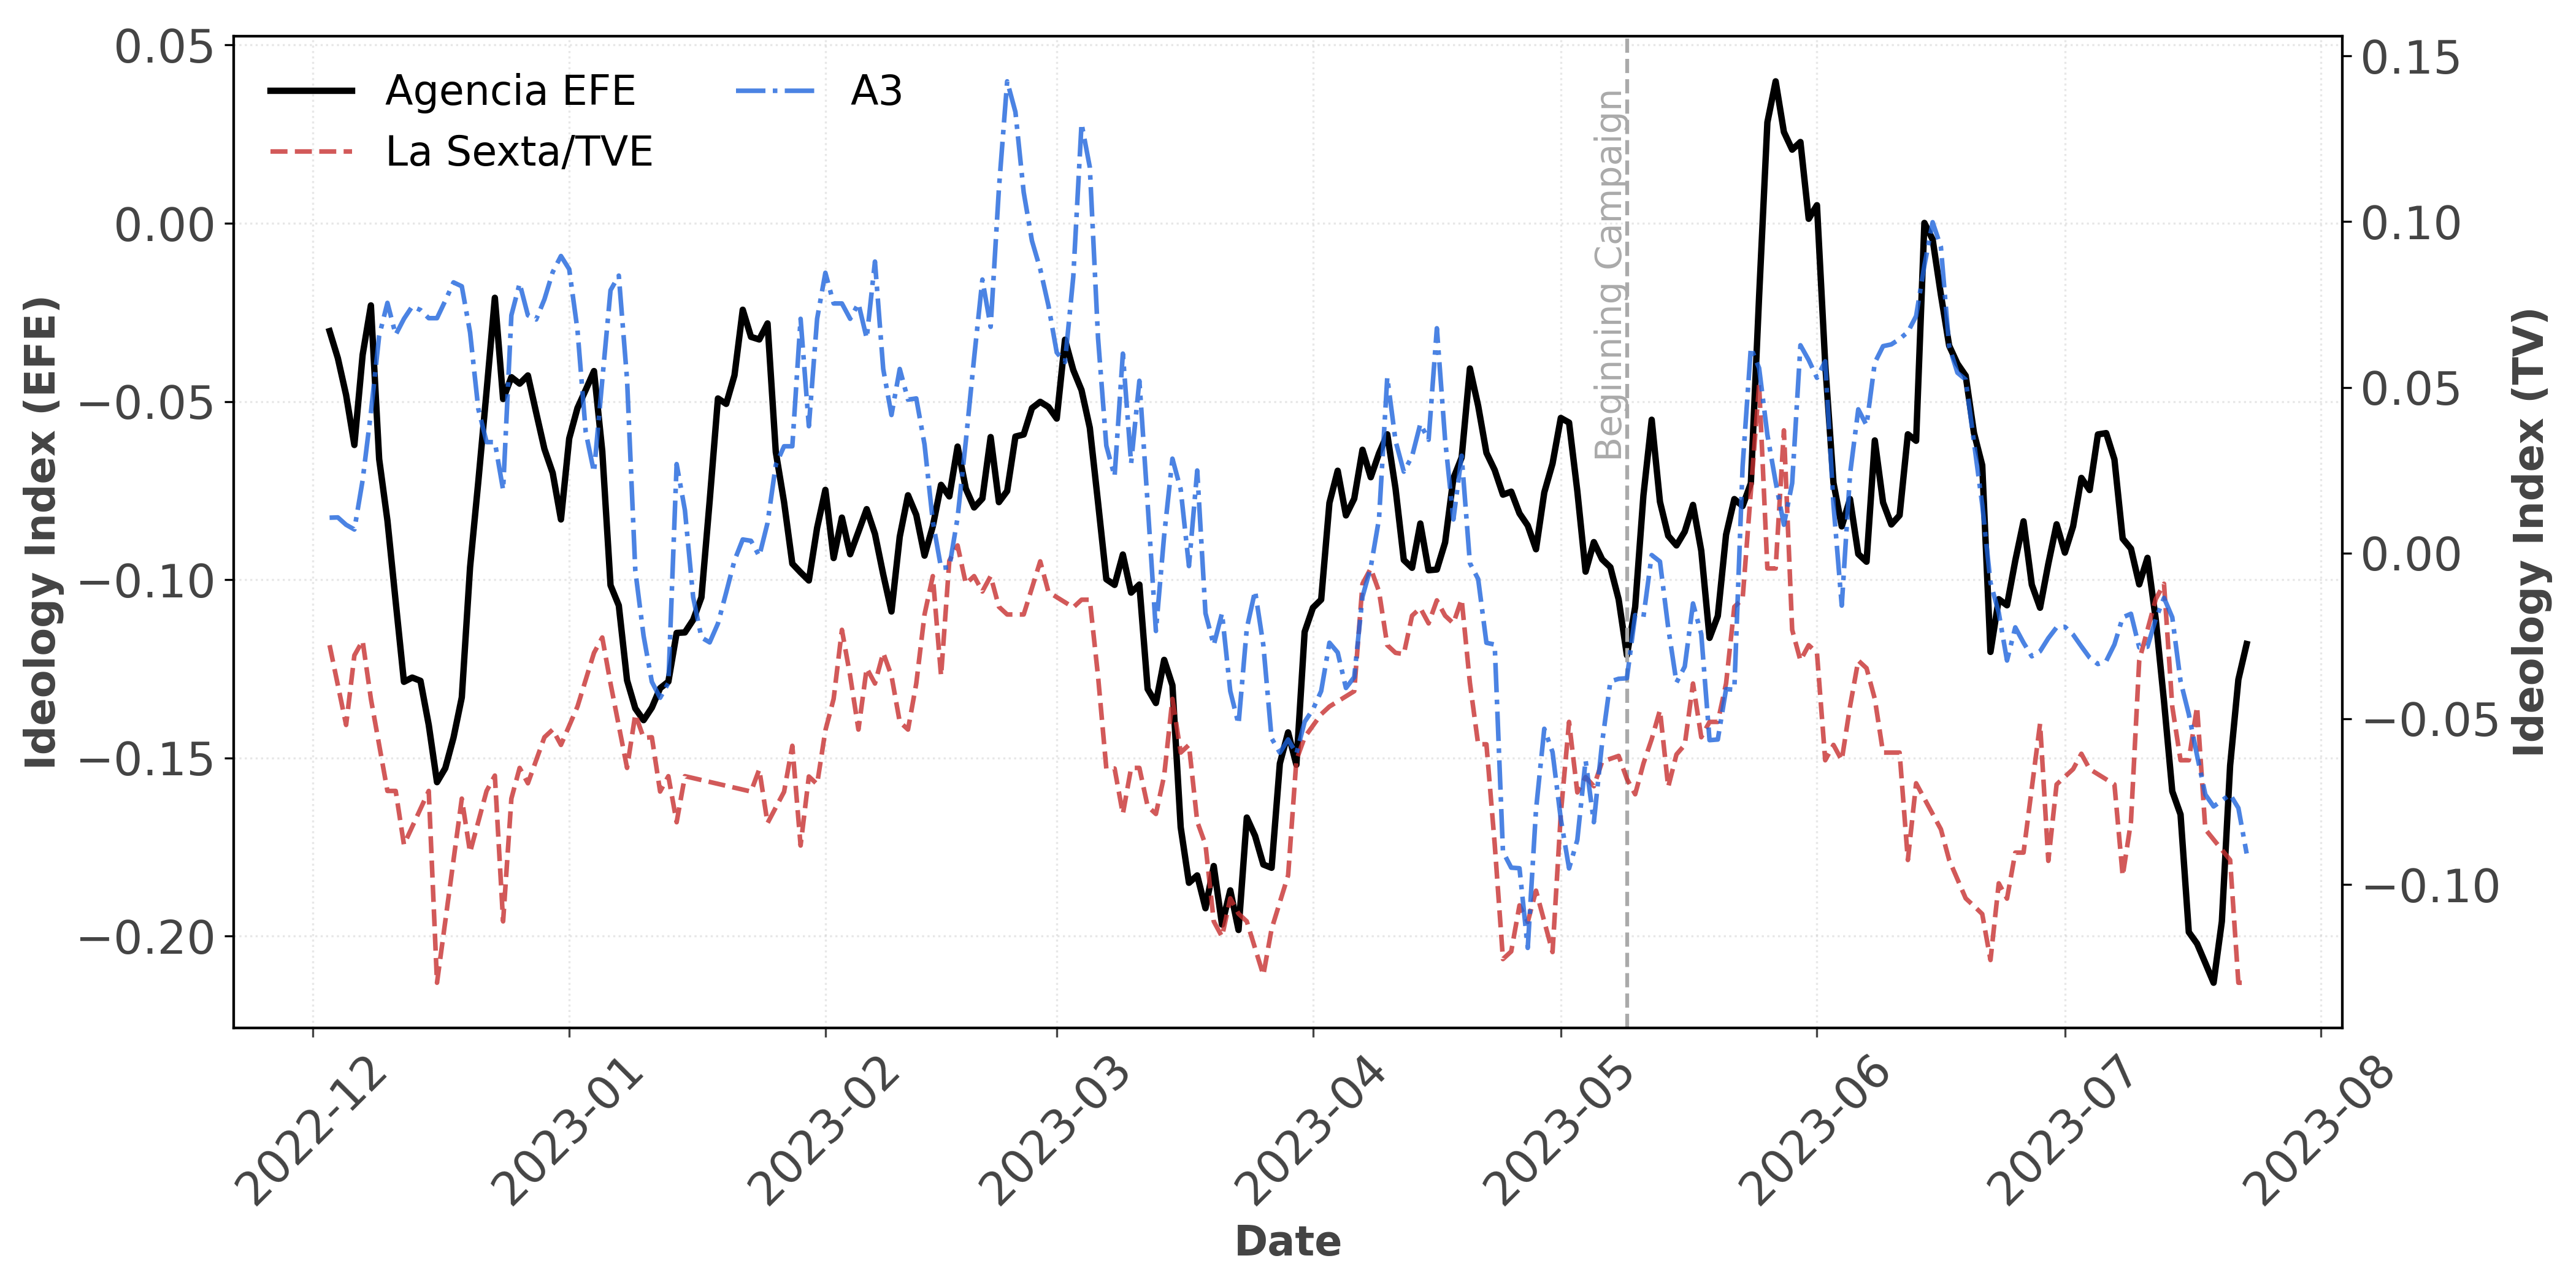
\includegraphics[width=150mm]{figures/tv_vs_efe_net_diff}
	\caption*{\small \textit{Note:} The figure represents the time series of slant index defined in Eq. \eqref{eq:ideo_index} for both the  TV outlets (right y-axis) and the newswire agency EFE (left y-axis). Positive values denote pro-right coverage; negative values denote pro-left coverage. TV channels are grouped into left-leaning (La Sexta and TVE) and the right-leaning (A3). All series are smoothed using a centered rolling mean with a 9-day window.}
	\label{fig:net_tone}
\end{figure}

%Finally, the figure suggests that there are swings around salient political events. For instance,  the late-May rightward swing (regional elections) is amplified by A3, and the early-March leftward dip (International Women’s Day and the failed no-confidence motion of the Right) is amplified by La~Sexta/TVE.  This motivates a closer, formal analysis of asymmetric responsiveness, which I develop in Section~\ref{sec:identification}.

%There are clear structural breaks in outlets’ trends. In March 2023, the right-leaning channel A3 experienced a marked shift in its slant index, with its previously conservative orientation converging toward that of the left-leaning outlets. This break coincided with a surge of negative stories about the right and positive coverage of the left. During this period, Spanish politics was dominated by a failed no-confidence motion initiated by the far-right party Vox, which exposed divisions on the right and left the opposition weakened. At the same time, conservative parties were on the defensive over a series of symbolic and institutional controversies—ranging from opposition to progressive laws on gender identity, euthanasia, and feminism, to accusations of obstructing judicial reform and mishandling pensions. In contrast, the governing left bloc emphasized favorable developments, including record employment figures, new housing legislation, and major industrial investments. A3 did not return to its previous level of conservatism until June, when the right’s strong performance in the May regional elections brought back the  divergence and partisan polarization between left- and right-leaning outlets.


There are clear structural breaks in outlets’ trends. In March 2023, the right-leaning channel A3 experienced a marked shift in its slant index, with its previously conservative orientation converging toward that of the left-leaning outlets. This break coincided with a surge of negative stories about the right and positive coverage of the left. At that time, coverage turned more negative for the right and more positive for the left. A failed no-confidence vote launched by the extreme-right party Vox exposed splits on the right and weakened the opposition. Right parties were also on the defensive over several issues: opposing new laws on gender identity, assisted dying, and gender equality; being accused of blocking judicial reform; and disputes over pensions. Meanwhile, the governing left highlighted favorable news—record employment, a new housing law, and major industrial investment announcements. The right wing outlet A3 did not return to its previous level of conservatism until June, when the right’s strong performance in the May regional elections brought back the  divergence and partisan polarization between left- and right-leaning outlets. 



For the analysis that follows, I take the entire off-campaign period as the baseline to better capture the underlying conservatism of A3. To illustrate how slant changed between the two periods of analysis, I decompose tone by party in Appendix Figure \ref{fig:tone_by_party}. During the campaign, all outlets adopted a common approach to the parties at the extremes: they became more negative toward the far-right party VOX and more positive toward the left-wing party SUMAR. As a result, cross-channel slant became slightly less dispersed, and outlets’ ideological positions converged.\footnote{Appendix Figure~\ref{fig:change_line} shows changes in left–right positions. Dispersion is summarized using three complementary statistics: the cross-channel range (distance between the most right- and most left-leaning outlet), the standard deviation (spread around the mean), and the left–right bloc gap (A3 versus the average of La Sexta, TVE, and T5). The cross-channel range declined from 0.088 to 0.083, the standard deviation from 0.032 to 0.030, and the bloc gap from 0.063 to 0.051.}




%My division of the two sample  consider all  the months before the beginning of the campaign as the base period. This aims at better capturing the underlying conservativism of the right wing channel A3. To summarize how slant changes were affected in these periods, I decompose tone by each of the political parties in Appendix Figure \ref{fig:tone_by_party} for both periods.  The campaign period marked a common strategy for all the outlets: : all outlets became more negative on the extreme-right party VOX and more positive on the left-wing party SUMAR.  This resulted in less segregated news landscape: outlets’ ideological positions converge modestly during the campaign. Quantitatively, dispersion across channels narrowed slightly during the campaign \footnote{Changes in outlet's left-right positions are depicted in Appendix Figure  \ref{fig:change_line}. Dispersion is summarized using three complementary statistics. The cross-channel range measures the distance between the most right- and most left-leaning outlet. The standard deviation summarizes overall spread across outlets relative to the mean. Finally, the left–right bloc gap compares the average position of A3 (the only right-leaning outlet) with the average of the three other channels (La Sexta, TVE, and T5).  The cross-channel range declined from 0.088 to 0.083, and the standard deviation from 0.032 to 0.030. Likewise, the left–right bloc gap (A3 versus the other three channels) fell from 0.063 to 0.051. }


%During the campaign, all outlets—including the newswire EFE—shifted in the same direction on two tone categories: negative-left coverage declined while negative-right coverage increased (Table \ref{tab:political_sentiment_types}). Furthermore, 




\begin{comment}
	content...

Research finds that attacks intensify during campaigns \citep{lau2009negative}, while news outlets propagate and magnify them \citep{iyengar_affective}, leading to more polarized news content.  In my setting, however, the opposite happens: the political spectrum becomes more homogeneous.   Figure \ref{fig:change_line} illustrates the movement from dots (off-campaign) to crosses (campaign). The newswire EFE (not shown in the figure) moved toward the right, shifting from –0.17 to –0.13. This movement was mirrored only by the publicly owned channel TVE, which repositioned toward the center, whereas all other outlets shifted to the left.\footnote{Average relative tone by period is shown in Appendix Figure \ref{fig:tone2}.}


	\begin{figure}[!htb]
		\centering
		\caption{Change in Positions Off-campaign to Campaign}
		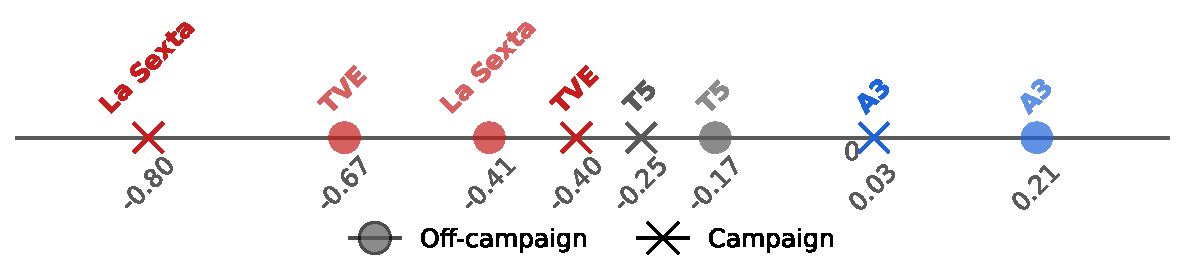
\includegraphics[width=100mm]{figures/congress_line_chatgpt_pre_postv2}
		
		\caption*{\small \textit{Note:} The figure shows the relative change in  slant positions  according to the ideological index in Equation \ref{eq:ideo_index} from off-campaign to campaign. 	}% Values are normalized so that the two most extreme positions take values -1 and 1 in the off-campaign period. }
		\label{fig:change_line}
	\end{figure}
	
	
Despite more politics, outlets’ ideological positions converge modestly during the campaign. Quantitatively, dispersion across channels narrowed slightly during the campaign\footnote{Dispersion is summarized using three complementary statistics. The cross-channel range measures the distance between the most right- and most left-leaning outlet. The standard deviation summarizes overall spread across outlets relative to the mean. Finally, the left–right bloc gap compares the average position of A3 (the only right-leaning outlet) with the average of the three other channels (La Sexta, TVE, and T5).}: the cross-channel range declined from 0.088 to 0.083, and the standard deviation from 0.032 to 0.030. Likewise, the left–right bloc gap (A3 versus the other three channels) fell from 0.063 to 0.051. 
	
\end{comment}
	
	
	
	
	
	
	
	
	

	
	
	\section{Demand for News}	\label{sec:demand}

In this section, I introduce the market setting for demand. I first develop a mixed logit (BLP) model \citep{berry_blp} where individuals choose the channel to watch depending on the content characteristic offered by the outlets (i.e., political slant). I then describe the endogeneity problem that arises from the simultaneity between editorial decisions and viewers' choices and introduce my identification strategy. Finally, I present the main estimation results and evidence linking media polarization to political polarization. 

	\subsection{Demand Model}



Since newscasts carry no advertising, I abstract from two-sided market considerations. Viewers choose a single outlet to watch the news or else choose the outside option, defined as not consuming any of them. The single-product choice assumption might be particularly strong in television markets, where viewers can easily switch programming during the broadcasts—something that cannot be identified from daily aggregate data. To mitigate this concern, I restrict attention to the initial (i.e., minute-zero) audience for each day.\footnote{Previous works have documented the importance of inertia from previous shows in TV news consumption \citep{richter2025structural}. During my sample period, there were no changes in the preceding slot's programming agenda, which minimizes this concern given the inclusion of day of the week fixed effects. Results are robust to the estimation using the first five minutes of the shows. } This makes the outlet choices mutually exclusive since they coincide in their broadcast emission times and thus cannot be simultaneously chosen. 



	I consider a market where both firms and products coincide. Formally, an individual $ i $  in region $r$ chooses between any outlet $ j \in \mathcal{J}\equiv \{La \ Sexta,TVE,T5,A3\}$  to watch at the beginning of day $d$ or the outside option ($j=0$). I define the expected utility of  $j$ as:
	
	
	\begin{equation}\label{eq:utility}
		\begin{aligned}
			& U_{ijrd}= \underbrace{\sum_k x_{jd-1}^k\beta^k+w_{rd}   \gamma  +  \xi_{jrd}}_{\delta_{jrd}}  + \underbrace{  \sum_k x_{jd-1}^k \Big( \sigma^k \nu_{ird}^k  + \pi^ky_{irm} \Big)}_{\mu_{ijrd}}+\epsilon_{ijrd} 
		\end{aligned}
	\end{equation} 
	
	and the one for the outside option is assumed to be $U_{i0}=\epsilon_{i0}$. The observed characteristics $ x_{jd}^k $ represent the  proportion of time on channel $ j $ and day $ d$ devoted to characteristic $ k \in \{R+,R-,L+,L-,political\}$ as defined in Eq. \eqref{eq:controls}. $w_{rd}$ measures the precipitation level on a given day-region. Weather shocks raise the utility of the inside options  relative to the outside option, making viewers more likely to engage in indoor activities such as TV consumption \citep{wilbur}. Individual taste shocks follow a standard normal distribution, $ \nu_{ird}^k \sim N(0,1)$, with mean shifted by  demographics, $ y_{irm} $, that represent whether individual $i$ in region $r$ is right-wing in month $m$ according to survey data.	Thus $\delta_{jrd}$ captures the mean utility for the baseline type (left-viewers) and the parameters $\pi^k$ allow for asymmetric tastes of politics based on ideology, enabling to test the degree of polarization in news consumption. 

The unobserved (to the econometrician) product characteristics are decomposed into $\xi_{jrd}= \xi_j + \xi_{dow} + \Delta \xi_{jrd}$, where I include product dummies that account for unobserved quality factors such as outlet loyalty, and day of the week dummies to control for  seasonal variation in the value of TV consumption. Other unobserved product shocks might include higher valuation of a given type of story that comes from knowledge of it through social media, specific regional taste shocks due to local events, etc. By assumption, viewers have full information about all the product characteristics when making decisions. %The outside option is modeled in terms of \textit{potential} audience  \citep{berry1994estimating} and its mean utility value is normalized to 0.


The market share for the $j$th product is computed as the integral over the individual choice indicators as: 
	
	
	\begin{equation}\label{eq:shares}
	\begin{aligned}
		& s_{jrd} = \int d_{ijrd}(\bm{\delta_{rd}},\bm{\mu_{ird}})d\bm{\mu}_{ird}d\bm{\epsilon}_{ird}
	\end{aligned} 
\end{equation} 
	
	where $d_{ijrd}$ equals $1$ if $U_{ijrd}>U_{ikrd} \quad \forall j\neq k$ and $0$ otherwise. The shocks $\epsilon_{ird}$ are assumed to be i.i.d. drawn from a type I extreme-value distribution.\footnote{The model is estimated using the \textit{pyblp} package \citep{conlon2020best}.} 

Under the assumption of no individual heterogeneity in preferences  ($\bm{\sigma}=0$) and a homogeneous ideology distribution ($y_{ir}= \bar{y}_r$),  Eq. \eqref{eq:utility} collapses to a plain logit model: 


\begin{equation}\label{eq:logit}
	\begin{aligned}
		& ln \left(\frac{s_{jrd}}{s_{0rd}}\right)= \sum_k x_{jd-1}^k\beta^k+w_{rd}   \gamma  +\sum_k \left(x_{jd-1}^k\times y_r \right) \phi^k +  \xi_{jrd}
	\end{aligned} 
\end{equation} 


I report results for both  BLP and  logit models in  Section \ref{sec:results}. 
	
	\subsection{Endogeneity and Identification Strategy} \label{sec:endogeneity}
	\label{sec:identification}
	
	
Models of demand estimation have often treated product characteristics as exogenous and used them as instruments for estimating price elasticities. That can be reasonable when characteristics are costly to adjust and competition is mostly price-based after product launch. In news markets, however, slant is endogenous since it is chosen by the outlets taking into account the same unobserved demand shocks that move audience shares.
	
	
	
	Formally, viewers form expectations about each channel’s utility to start watching the news on day $d$ based on exogenous variables—weather, individual attributes, and an unobserved (to the econometrician) shock~$\xi$—as well as yesterday’s  realized slant content ~$\bm{x}_{jd-1}$. Channels already choose day's $d-1$ slant while forming expectations about next-day utility shocks~$\Delta\xi_{j,d}$. These shocks have two components.
	
	
	On the one hand, there are day $d$ taste shocks that outlets did not foresee when they set yesterday's slant.  These include information people acquire on the day through social media about political events, which can raise the immediate payoff from starting the news on a particular outlet. The timing difference partially addresses this concern because at minute–0 viewers choose a channel to start consuming the news based on exogenous factors and on yesterday’s slant $\bm{x}_{j,d-1}$, which has already occurred. Hence these shocks that shift minute–0 utility are orthogonal to $\bm{x}_{j,d-1}$ due to timing differences and do not create endogeneity in the estimation of the preferences for slant coefficients.
	
	
On the other hand, there are predictable components—ongoing scandals, pre-show information—that outlets can anticipate and incorporate when planning and setting slant. As a result,  optimal content decisions are functions of these anticipated taste shocks, implying $\E[\mathbf{x}_{jrd-1}\,\Delta\xi_{jrd}] \neq \mathbf{0}$.
	

	I address endogeneity using random variation in the daily composition of the story pool available to produce the news. Each day’s newswire feed is a proxy for the set of stories editors can draw on to build the newscast. The political mix of this set determines what is newsworthy and thus constrains what outlets can speak about. Although these shocks are common to all outlets, they affect outlets asymmetrically. Since events are not predictable and outlets wish to maintain their stance, they need to take advantage of politically "favorable" days where they can increase the coverage of events that match their political leaning. I therefore use the \emph{news shock} $\mathbf{z}_d$ defined in Eq.~\eqref{eq:efe} as instruments for outlet–day slant $\mathbf{x}_{jd}$. The key identification assumption is that $\mathbf{z}_d$ affects audience shares only through its impact on the cost of supplying slanted content, not through direct shifts in viewers’ tastes.
	
	
	
%I address this endogeneity by using the daily composition of the newswire content as an exogenous supply shock. Each day's wire composition serves as a baseline for what the outlets have available to start producing their newscast. Exogenous shocks to this baseline determine what is newsworthy and thus constrain what outlets can speak about. I use the \emph{news shock} $\mathbf{z}_d$ defined in Eq.~\eqref{eq:efe} as instruments for outlet–day slant $\mathbf{x}_{jd}$. Although these shocks are common for all the outlets, they are asymmetrically affected by them. Since they want maintain preferred slant positions, but in the short run the available story mix constrains coverage, so they smooth shocks and take advantage of “favorable” days. The key identification assumption is that $\mathbf{z}_d$ affects audience shares only through its impact on the cost of supplying slanted content, not through direct shifts in viewers’ tastes.
	
	
	
The following examples illustrate the mechanism.\footnote{The full breakdown of the text examples is shown in Tables \ref{tab:neg_left_channels} and \ref{tab:neg_right_channels}.} On {27 February 2023} (the highest $z_d^{L-}$ in the sample), a loophole in a law sponsored by UP led to early releases of convicted sexual offenders and corruption scandals hurt the Socialist Party. Airtime given to negative left-wing stories differed markedly across channels: A3 (right) devoted almost 19\%, TVE (left) and T5 each gave roughly 4\%, and La Sexta (left) about 2\%. The mirror image occurred on {17 May 2023} (the most negative day for right-wing parties): stories included a payments scandal involving the right-wing People’s Party, the defeat of a conservative motion in the Senate, and police-abuse allegations during a march against the extreme-right party VOX. Left-leaning outlets devoted about 15\% of airtime to negative right-wing content, whereas the right one devoted roughly 4\%. 

	
	
%The \emph{news shock} \(\bm{z}_d\) as defined in Eq. \ref{eq:efe},     is common to all outlets  but affects them asymmetrically. Channels would like to produce at their steady-state, average positions, but in the short run the available story mix constrains what they can cover. Since the news landscape varies randomly, they smooth out variations in the news landscape by taking advantage of favorable days. The main identification assumption is that conditional on day of the week fixed effects and controls, $\mathbf{z}_d$ shifts audience shares only through its effect on the cost of supplying slanted content (i.e., through $\mathbf{x_{jd}}$), not through direct shifts in viewers’ tastes.




	
 To show formal evidence of the previous mechanism, for each $(\text{party},\text{tone})$ pair I estimate separate regressions of the form:
	
	
	

	
	\begin{comment}
	\begin{figure}[h!]
		\caption{Trade-offs in the model}
		\label{fig:diagram}
		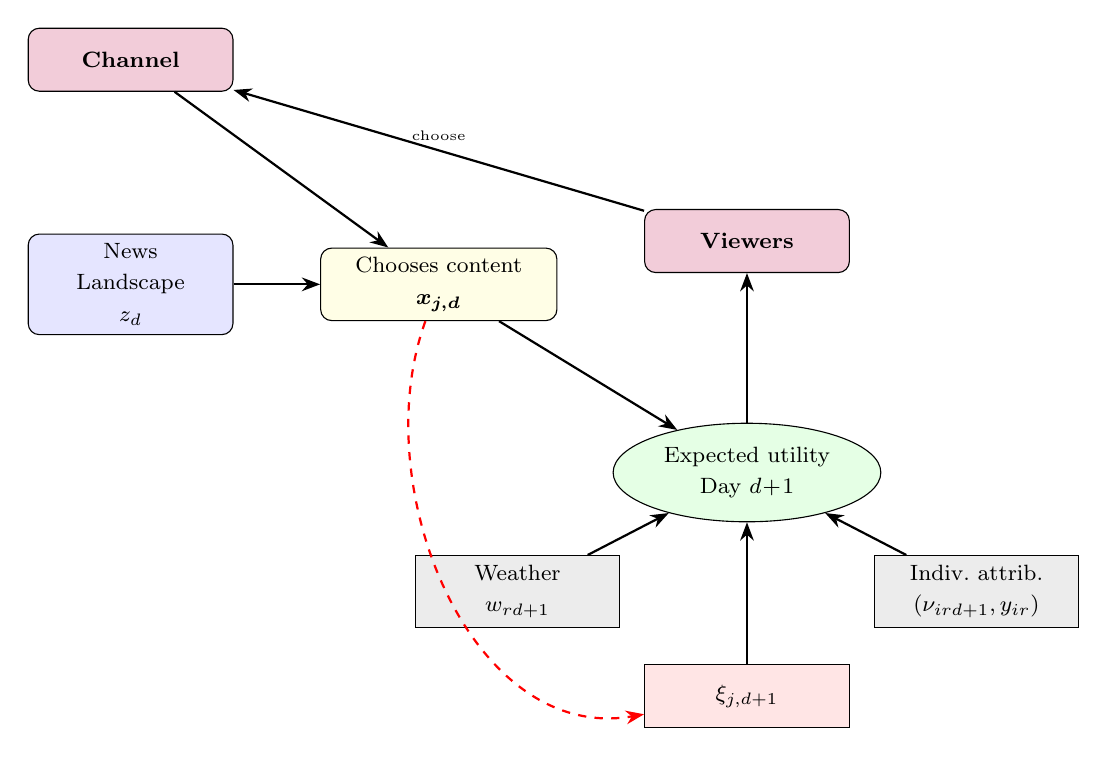
\begin{tikzpicture}[
			inst/.style   ={rectangle, draw, fill=blue!10,  rounded corners, align=center,
				minimum width=2.6cm, minimum height=0.8cm},
			decision/.style={rectangle, draw, fill=yellow!10, rounded corners, align=center,
				minimum width=3.0cm, minimum height=0.9cm},
			util/.style   ={ellipse,   draw, fill=green!10,  align=center,
				minimum width=3.4cm, minimum height=1.0cm},
			shock/.style  ={rectangle, draw, fill=red!10,   align=center,
				minimum width=2.6cm, minimum height=0.8cm},
			exo/.style    ={rectangle, draw, fill=gray!15,  align=center,
				minimum width=2.6cm, minimum height=0.8cm},
			actor/.style  ={rectangle, draw, fill=purple!20, rounded corners, align=center,
				minimum width=2.6cm, minimum height=0.8cm},
			flow/.style   ={-Stealth, thick},
			feed/.style   ={dashed,-Stealth, thick, red},
			node distance = 1.8cm and 1.1cm,
			font=\footnotesize
			]
			% -------- DAY d (supply) ---------
			\node[inst]                    (news)   {News\\Landscape\\$z_{d}$};
			\node[actor, above=of news]    (channel) {\textbf{Channel}};
			
			\node[decision, right=of news] (x)      {Chooses content\\$\bm{x_{j,d}}$};
			
			% -------- DAY d+1 (demand) ------
			\node[actor, right=of x, yshift=0.55cm] (viewer) {\textbf{Viewers}};
			
			\node[util,  below=of viewer, yshift=-0.1cm] (util)
			{Expected utility\\Day $d\!+\!1$};
			\node[shock, below=of util]     (xi)     {$\xi_{j,d+1}$};
			\node[exo,   below left=0.6cm and 0.4cm of util]
			(weather){Weather\\$w_{rd+1}$};
			\node[exo,   below right=0.6cm and 0.4cm of util]
			(prefs)  {Indiv.\ attrib.\\$(\nu_{ird+1},y_{ir})$};
			
			% ---------- flows ---------------
			\draw[flow] (channel) -- (x);
			\draw[flow] (news)    -- (x);
			\draw[flow] (x)       -- (util);
			\draw[flow] (prefs)   -- (util);
			\draw[flow] (weather) -- (util);
			\draw[flow] (xi)      -- (util);
			\draw[flow] (util)    -- (viewer) node[midway,right,font=\tiny]{};
			\draw[flow] (viewer)    -- (channel) node[midway,above,font=\tiny]{choose};
			
			
			% ------ anticipation feedback ---
			\draw[feed] (x) to[out=-110,in=190] node[midway,below,font=\tiny]
			{} (xi);
		\end{tikzpicture}
		\caption*{\small
			Notes: This diagram illustrates the structure of the model. Solid black arrows indicate causal and temporal dependencies among variables. The red dashed arrow emphasizes the simultaneity problem: content decisions $\bm{x}_{j,d}$ are made with knowledge of the future utility shock $\xi_{j,d+1}$.
		}
		
	\end{figure}
	
	
	\end{comment}


%That there is exogenous variation across outlets is of practical importance for estimation and a necessary requirement that  the  rank condition requires for identification \citep{berry_haile_econometrica}. In order to show formal evidence of this variation,  I estimate, for each $(party,tone)$ pair, separate regressions of the form:
\begin{equation}\label{eq:first_stage}
	\begin{aligned}
		 x^{party, tone}_{jd} =	\sum_{k} \sum_{j'}
		\left(d_j(j') \times z^{k}_d\right)\,\alpha_{j}^{k}
		+ \gamma_{dow}+\epsilon_{jd},
	\end{aligned}
\end{equation}

where $k \in\{L+,R+,L-,R-, political\}$. As defined in Eq. \eqref{eq:controls},  $x^{party, tone}_{jd}$ is outlet $j$’s share of airtime with positive or negative tone about $party \in \{L,R\}$;  $z^{k}_d$ is the corresponding news shock from Eq. \eqref{eq:efe}, and $d_j(j')$ is a dummy with value one if $j=j'$ and $\gamma_{dow}$ are day of the week fixed effects.  Controlling for the whole news landscape, I estimate how outlets increase the production of each type of content.
A positive coefficient $\alpha_{j}^{R+}$ means that, ceteris paribus, a 1 p.p. increase in  positive right-wing news shock increases outlet $j$’s coverage of the right by $\alpha_{j}^{R+}$ p.p.


Figure \ref{fig:fwl} presents added-variable plots for regression Equation  \eqref{eq:first_stage}  pooling left channels for simplification.\footnote{I also present a non-linear LOWESS version to mitigate concerns of outliers in Appendix Figure \ref{fig:fwl_lowess}. Full results of the estimation are shown in Table \ref{tab:first_stage}.} Outlets generally respond to news shocks by increasing their coverage, independently on whether these affect  right or left parties. The difference therefore, lies on the intensive margin: when the share of  positive-right stories rises by one standard deviation, the right-leaning A3 lifts its own positive-right airtime by about 0.24 stdev., whereas the left-leaning outlets TVE and La Sexta react hardly at all.  Symmetrically, a one-stdev. increase in positive-left stories leads TVE to expand favorable coverage of the left by roughly 0.26 stdev, while A3’s response is 0.13 stdev.  By contrast, the adjustment on the negative right content is small and non-significant. This is consistent with a saturation effect. Since all outlets already use negative tone on the right  (e.g., see Figure \ref{fig:chat}) this leaves them with less margin to adjust on this category. 





% Figure \ref{fig:fwl} presents added-variable plots for regression Equation  \eqref{eq:first_stage} \footnote{I also present a non-linear LOWESS version to mitigate concerns of outliers in Appendix Figure \ref{fig:fwl_lowess}. Full results of the estimation are shown in Table \ref{tab:first_stage}.} pooling left channels for simplification.  When the share of  positive-right stories rises by one standard deviation, the right-leaning A3 lifts its own positive-right airtime by about 0.30 stdev., whereas the left-leaning outlets TVE and La Sexta react hardly at all.  Symmetrically, a one-stdev. increase in positive-left stories leads TVE to expand favorable coverage of the left by roughly 0.38 stdev, while A3’s response is not statistically different from zero.   By contrast, the adjustment on the negative right content is small. This is consistent with a saturation effect. Since all outlets already use negative tone on the right  (e.g., see Figure \ref{fig:chat}) this leaves them with less margin to adjust on this category. 
 

	
	
		\begin{figure}[!htb]
		\centering
\caption{Added Variable Plots for Production of Political Content}
		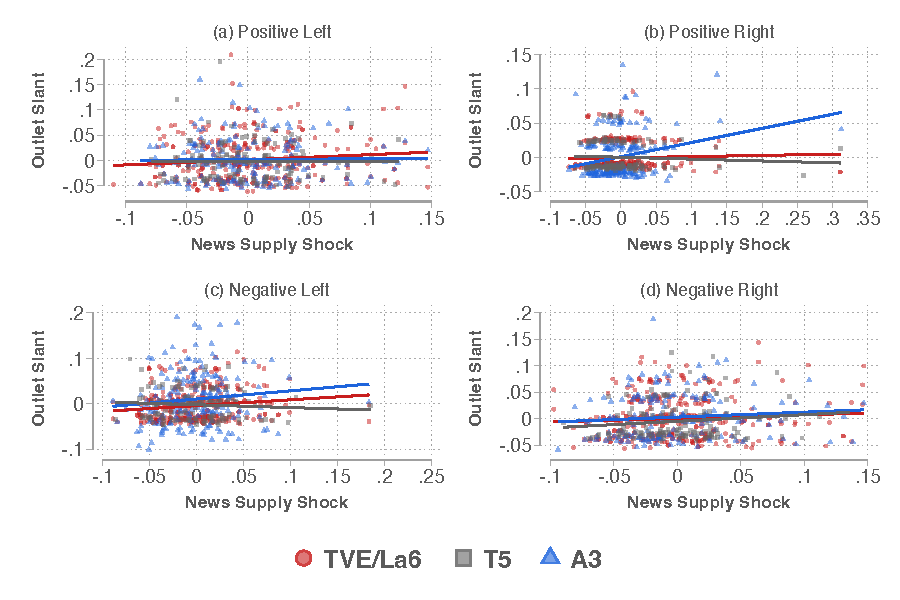
\includegraphics[width=160mm]{figures/fwl_plots_v2}
		\caption*{\small \textit{Note:} The figure shows the added variable plots from the estimation of regression Equation \eqref{eq:first_stage}. The x-axis represents the news shocks $z_d^k $ residuals and the y-axis the corresponding outlet's slant $x_{jd}^k $ residuals for each party-tone combination. Channels are pooled into left (TVE and La Sexta), middle (T5) and right (A3) for visualization purposes.  }
		\label{fig:fwl}
	\end{figure}
	
		The existence of exogenous variation in outlets' response to the common news' shock is required by the rank condition in the estimation \citep{berry_haile_econometrica}.  Table \ref{tab:tests}   shows the F test for equality of coefficients across all outlets and the t-test for equality between right- and left-leaning outlets. The largest and most significant differences occur for pro-right content, followed by negative left, positive left and, the less significant negative right. 
	
	
	
	\begin{table}[!htbp]
		\centering
	

		\caption{Tests for Differences in Coefficients}
		\begin{tabular}{lcccc}
			\hline
			Characteristic & F-test  & F-test p-value & T-test  & T-test p-value \\
			\hline
			$ {L-}$& 2.69 & 0.07 & 3.51  & 0.06 \\
			$ {L+}$ & 1.31 & 0.27 & 1.87  & 0.17 \\
			$ {R-}$ & 0.42 & 0.66 & 0.34 & 0.56 \\
$ {R+}$ & 8.78 & 0.00 & 17.55  & 0.00 \\
			\hline
		\end{tabular}
			\caption*{\small \textit{Note:} Summary of F- and T-test results for equality of coefficients across channels from regression Equation \eqref{eq:first_stage}. The F-test evaluates overall equality across channels, while the T-test compares the coefficient of the main independent variable between A3 and TVE/La Sexta.}
					\label{tab:tests}
	\end{table}
	

	
		
	
	Accordingly, I use
	$\bm{z}_{d}$
	as instruments for the linear content characteristics $ \bm{x}_{jd}$.  For the $K$ non-linear parameters governing preference heterogeneity $ \bm{\sigma}$, I follow \citet{gandhi2019measuring} and use instruments of the form 
	$\bigl(\hat{x}_{jd}^k-\sum_{l\neq j}\hat{x}_{ld}^k\bigr)^2$,
	where $\hat{x}_{jd}^k$ is the predicted slant based on the reduced-form regression Eq.~\eqref{eq:first_stage}. 	To identify the demographic interaction coefficients $\pi$, I multiply these instruments by the average share of right-wing votes, $\bar y_{mr}\,\hat{x}_{jd}^k$.



	\subsection{Results of the Demand Estimation}
	
	\label{sec:results}
	
	
I present the results of the BLP estimation for the off-campaign and campaign periods in Table \ref{tab:results_blp}. I show the preferred specification with both outlet and day-of-week fixed effects, and standard errors clustered at the regional level. Because the political division in demographics is only between left- and right-leaning viewers, the \(\beta\)s represent the mean tastes of left-leaning viewers and the \(\pi\)s are deviations for right-leaning audiences.


\begin{table}[!htbp]
	\caption{BLP Estimation Results with Standard Errors}
	\label{tab:results_blp}
	\centering
	\begin{threeparttable}
		\begin{tabular}{lccc}
			\hline
			\textbf{Coefficient} & \textbf{Parameter} & \textbf{Estimate} & \textbf{Std. Error} \\
			\hline
			\multicolumn{4}{c}{Off-campaign} \\
			\hline
			\hline
			Positive Left & $\beta^{L+}$ & -16.90 & (11.73) \\
			Positive Right & $\beta^{R+}$ & -25.53 & (31.03) \\
			Negative Left & $\beta^{L-}$ & 28.29 & (25.89) \\
			Negative Right & $\beta^{R-}$ & 56.44** & (28.45) \\
			Political & $\beta^{political}$ & 11.49*** & (4.28) \\
			Weather & $\gamma$ & 0.00 & (0.03) \\
			\hline
			Positive Left & $\sigma^{L+}$ & 0.44 & (296.90) \\
			Positive Right & $\sigma^{R+}$ & 0.68 & (715.26) \\
			Negative Left & $\sigma^{L-}$ & 12.64 & (8.68) \\
			Negative Right & $\sigma^{R-}$ & 21.99 & (13.83) \\
			Political & $\sigma^{political}$ & 0.00 & (46.79) \\
			\hline
			Right-Wing $\times$  Positive Left & $\pi^{L+}$ & 46.26 & (48.70) \\
			Right-Wing $\times$  Positive Right & $\pi^{R+}$ & 77.81 & (95.92) \\
			Right-Wing $\times$  Negative Left & $\pi^{L-}$ & -70.09 & (57.97) \\
			Right-Wing $\times$  Negative Right & $\pi^{R-}$ & -103.71 & (97.76) \\
			Right-Wing $\times$  Political & $\pi^{political}$ & -25.17** & (12.59) \\
			\hline
			\hline
			\multicolumn{4}{c}{Campaign} \\
			\hline
			\hline
			Positive Left & $\beta^{L+}$ & 134.16** & (65.57) \\
			Positive Right & $\beta^{R+}$ & -129.79*** & (48.43) \\
			Negative Left & $\beta^{L-}$ & -104.84** & (41.32) \\
			Negative Right & $\beta^{R-}$ & 92.62** & (41.63) \\
			Political & $\beta^{political}$ & -6.43** & (3.26) \\
			Weather & $\gamma$ & 0.00 & (0.01) \\
			\hline
			Positive Left & $\sigma^{L+}$ & 0.00 & (320.36) \\
			Positive Right & $\sigma^{R+}$ & 19.25* & (10.89) \\
			Negative Left & $\sigma^{L-}$ & 0.00 & (134.33) \\
			Negative Right & $\sigma^{R-}$ & 0.02 & (73.18) \\
			Political & $\sigma^{political}$ & 0.00 & (19.55) \\
			\hline
			Right-Wing $\times$  Positive Left & $\pi^{L+}$ & -421.99** & (176.15) \\
			Right-Wing $\times$  Positive Right & $\pi^{R+}$ & 334.94*** & (127.41) \\
			Right-Wing $\times$  Negative Left & $\pi^{L-}$ & 288.65** & (116.22) \\
			Right-Wing $\times$  Negative Right & $\pi^{R-}$ & -280.33*** & (104.44) \\
			Right-Wing $\times$  Political & $\pi^{political}$ & 19.34** & (8.93) \\
			\hline
			\hline
		\end{tabular}
		
		
		
		
		\caption*{\small \textit{Note:} The table shows the results of the BLP estimation of model \eqref{eq:utility}. The estimations are divided into the off-campaign and campaign period. Both day-of-the-week and outlet fixed effects are included. Standard errors are clustered at the region level. The total number of observations are $N_{campaign}=2307$ and  $N_{off-campaign}=6604$.}
		
	\end{threeparttable}
\end{table}




Most of the heterogeneity is captured by the demographics (i.e ideology).  The estimated taste-dispersion parameters (\(\sigma\)s) are small and very imprecise. The high standard errors on these coefficients arise by construction. The identification of the random-coefficients  relies on variation across markets in the choice set, which is null in my case given that the same products are present across regions and dates.\footnote{A similar result was documented by \citet{Nevo1998MeasuringMP} for the cereal industry. Consistent with his findings, the relative importance of demographics versus random shocks—computed as the ratio of variance explained by demographics to the total variance in the distribution of estimated coefficients—exceeds 90\% in my model.} The low values of the  estimated $\sigma$s naturally link to the similar results that I obtain under the multinomial logit specification shown in Table \ref{tab:logit}. 
 
  In order to give a better interpretation of the content-taste parameters I present the mean own elasticities for both the off-campaign and campaign periods.   Given that increasing the positive relative minutes to a party also implies increasing the overall total minutes on politics, I compute the mean elasticity for the $k$-th characteristic as: 

%The pre-campaign estimates reveal four main facts. First, left-leaning audiences display a strong and precisely estimated mean taste for political stories (\(\beta^{political}>0\)). Second, left-wing viewers are pulled by negative tone on both blocs, with the effect much stronger and significant when the right bloc is the target (\(\beta^{R-}>0\)), while positive-toned stories are, on average, unattractive. Third, estimated taste-dispersion parameters (\(\sigma\)s) are small and very imprecise, which is unsurprising given that random-coefficient identification is weak when the set of products is fixed across markets \citep{berry_haile_econometrica}\footnote{These low values of heterogeneity naturally link to the similar results that I obtain under the plain logit specification shown in Table \ref{tab:logit}.}. Fourth, ideology–content interactions are generally noisy; the main signal is that right-leaning viewers place a lower value on generic political coverage than left-leaning viewers (\(\pi^{political}<0\)). 

%During the campaign window, the average taste of left audiences for political coverage turns negative (\(\beta^{political}<0\)), consistent with saturation once the race is underway. Framing now matters sharply: viewers reward positive stories about the left and negative stories about the right while penalizing the opposite frames, implying an aggregate tilt toward left-leaning parties (\(\beta^{L+}>0\), \(\beta^{R-}>0\), \(\beta^{R+}<0\), \(\beta^{L-}<0\)). Ideology interactions reveal marked polarization, with significant taste differences between right and left viewers. Right-leaning viewers now strongly seek favorable coverage of their own side and avoid negative stories about it (large opposing signs on \(\pi^{R+}\) and \(\pi^{R-}\)), dislike positive coverage of the left (\(\pi^{L+}<0\)), and demand negative coverage of the left (\(\pi^{L-}>0\)), indicating that out-group animosity is an important driver of viewing during the campaign.

	
%My results are consistent with \cite{Peterson2017Echo}, who found that partisans gravitate toward like-minded political content  during the 2016 U.S. presidential campaign. 


	
	
	

	
	
	\begin{comment}
		content...

	I present the results of the BLP estimation for the pre-campaign and campaign periods in Table \ref{tab:results_blp}. I show the preferred specification with outlet and day-of-week fixed effects and standard errors clustered at the regional level.
	
	The pre-campaign estimates reveal four main facts. First, there is a strong, statistically precise mean taste for stories about national politics in left audiences ($\beta^{political}$), indicating that political coverage per se draws audience attention before the campaign begins. Second, conditional on this baseline, viewers demand a negative tone toward both parties, but the pull is considerably stronger when the right-wing bloc is the target, whereas positive-toned stories are, on average, unattractive. Third, there is no sizable dispersion in the taste parameters captured by the estimated $\sigma$. This is expected, as identification of these parameters requires exogenous changes in the choice sets \citep{berry_haile_econometrica}, which do not apply in my market setup (i.e there are always the same amount of channels). Fourth, the ideology–content interaction terms are small and imprecise, so the heterogeneity cannot be explained by viewers’ ideology.
	
	During the campaign window, the same specification paints a markedly different picture. The average taste for political coverage becomes negative, suggesting that left audiences experience saturation once the race begins. Preferences reverse and intensify: viewers now reward positive stories about the left and negative stories about the right while penalising the opposite frames, producing an aggregate tilt toward left-leaning parties. Ideology–content interactions, however, reveal stark polarisation. Right-wing audiences actively seek favourable coverage of their own side and avoid negative stories about it, yet the dominant force is out-group animosity: they exhibit a particularly strong demand for negative coverage of the opposition. This pattern is consistent with \emph{affective polarisation} and echoes evidence from the United States showing that exposure to presidential campaigns makes partisans increasingly hostile toward their opponents \citep{Peterson2017Echo}.
		\end{comment}
	
	
	
	
	

	

	
	
	
	\begin{comment}
	
	\begin{table}[ht]
		\centering
		\begin{threeparttable}
			\begin{tabular}{lccc}
				\hline
				\textbf{Coefficient} & \textbf{Parameter} & \textbf{Estimate} & \textbf{Std. Error} \\
				\hline
				\hline
				\multicolumn{4}{c}{{Pre-campaign}} \\
				\hline
				\hline
				Positive Left & $\sigma^{L+}$ & 7.04 & (21.28) \\
				Positive Right & $\sigma^{R+}$ & 23.82 & (20.06) \\
				Negative Left & $\sigma^{L-}$ & 3.85 & (11.56) \\
				Negative Right & $\sigma^{R-}$ & 25.42*** & (5.01) \\
				Political & $\sigma^{\text{political}}$ & 3.47 & (7.58) \\
				\hline
				Right-Wing $\times$ Positive Left & $\pi^{L+}$ & 21.75 & (16.78) \\
				Right-Wing $\times$ Positive Right & $\pi^{R+}$ & 35.74 & (43.73) \\
				Right-Wing $\times$ Negative Left & $\pi^{L-}$ & -48.27 & (33.58) \\
				Right-Wing $\times$ Negative Right & $\pi^{R-}$ & -63.86 & (48.13) \\
				Right-Wing $\times$ Political & $\pi^{\text{political}}$ & -13.89 & (12.77) \\
				\hline
				Positive Left & $\beta^{L+}$ & -10.88 & (7.41) \\
				Positive Right & $\beta^{R+}$ & -18.19 & (23.08) \\
				Negative Left & $\beta^{L-}$ & 14.41 & (12.51) \\
				Negative Right & $\beta^{R-}$ & 43.11*** & (16.62) \\
				Political & $\beta^{\text{political}}$ & 4.73 & (5.41) \\
				Weather & $\gamma$ & 0.01 & (0.01) \\
				\hline
				\hline
				\multicolumn{4}{c}{{Campaign}} \\
				\hline
				\hline
				Positive Left & $\sigma^{L+}$ & 1.26 & (145.13) \\
				Positive Right & $\sigma^{R+}$ & 33.40 & (42.70) \\
				Negative Left & $\sigma^{L-}$ & 0.38 & (218.79) \\
				Negative Right & $\sigma^{R-}$ & 0.54 & (226.19) \\
				Political & $\sigma^{\text{political}}$ & 2.92*** & (0.90) \\
				\hline
				Right-Wing $\times$ Positive Left & $\pi^{L+}$ & -708.11** & (299.27) \\
				Right-Wing $\times$ Positive Right & $\pi^{R+}$ & 508.87*** & (172.30) \\
				Right-Wing $\times$ Negative Left & $\pi^{L-}$ & 413.36*** & (147.90) \\
				Right-Wing $\times$ Negative Right & $\pi^{R-}$ & -455.86** & (178.69) \\
				Right-Wing $\times$ Political & $\pi^{\text{political}}$ & 27.60** & (12.62) \\
				\hline
				Positive Left & $\beta^{L+}$ & 217.09*** & (76.90) \\
				Positive Right & $\beta^{R+}$ & -190.52** & (89.31) \\
				Negative Left & $\beta^{L-}$ & -145.58*** & (48.63) \\
				Negative Right & $\beta^{R-}$ & 147.49*** & (52.60) \\
				Political & $\beta^{\text{political}}$ & -10.80** & (4.89) \\
				Weather & $\gamma$ & 0.04 & (0.03) \\
				\hline
				\hline
			\end{tabular}
			\caption{BLP Estimation Results with Standard Errors}
							\label{tab:results_blp_updated}
			\begin{tablenotes}
				\small
				\item \footnotesize{The table shows the results of the BLP estimation of model \ref{eq:utility}. The estimations are divided in the pre-campaign and campaign period. Both day of the week and outlet fixed effects are included. Standard errors are clustered at the region level. The total number of observations is $N_{campaign}=2307$ and $N_{pre\_campaign}=6604$.}
			\end{tablenotes}
		\end{threeparttable}

	\end{table}
	
	\end{comment}
	
	
	%\subsubsection{Elasticities}
	
	%I present the mean own elasticities for both the off-campaign and campaign periods.   Given that increasing the positive relative minutes to a party also implies increasing the overall total minutes on politics, I compute the elasticity for the $k$th characteristic as: 
	
	\begin{equation}\label{eq:elasticities}
		\begin{aligned}
			& \bar{\epsilon}^k= \frac{1}{J\times R \times D}\sum_{j}\sum_{r} \sum_{d} \left(\frac{\partial s_{jrd}}{\partial x_{jt}^k} +  \frac{\partial s_{jrd}}{\partial x_{jt}^{political}} \right) \frac{x_{jd}^k}{s_{jrd}}    \quad \forall k \in \{R+,R-,L+,L-\}
		\end{aligned}
	\end{equation}             
	
	where aggregation is taken over outlets $(j)$, regions $r$ and days $d$.	Both left and right parties were almost equally disliked during off-campaign (Table \ref{tab:elasticities0}.). An increase of 1 percent in net tone  towards right (left) parties results in drops of 0.98 (1.00) percentage points in audience share; corresponding to a decrease of nearly 13,000 viewers.\footnote{A 1 p.p. increase in airtime on characteristic $k$ changes audience share by $\Delta S = S \times \tfrac{\epsilon}{100}$. Given an average total audience of $\bar{L}$, the level change in viewers is $\Delta V = \Delta S \times \bar{L}$. Since 1 p.p. of airtime corresponds to $0.01\,\bar{T}$ minutes (where $\bar{T}$ is the average broadcast length), $\tfrac{\Delta V}{\Delta t} = \bigl(S \times \tfrac{\epsilon}{100} \times \bar{L}\bigr) \times \tfrac{1}{0.01\,\bar{T}}$ gives the change in viewers per extra minute of coverage.} This is consistent with a taste for scandals or entertainment-like type of political content. During the campaign, aversion to right-leaning tone persists but weakens ($-0.60$ pp), and higher net tone on the left yields a small audience gain of 0.09 p.p. (867 viewers).
	
	
		 I focus now on the results for the main period of analysis, the election campaign. To see the extent of polarization in news consumption, I  compute elasticities for right and left markets separately. I define a “right market” as any region whose mean intention-to-vote to the right  ($\bar{y}_r$) lies above the median.  Figure~\ref{fig:elasticities_campaign} plots the estimated elasticities for that period for left markets (panel a) and right markets (panel b).\footnote{Table~\ref{tab:elasticities} and 	 Figure~\ref{fig:elasticities_pre} show full results also for the off-campaign period. }	Polarization becomes now evident. Left viewers present negative taste for content that harms their party and positive taste for content that benefits it. The analogous pattern is present in the taste of right-wing viewers. This campaign pattern contrasts with the off-campaign “scandal/negativity” taste, where both blocs reacted similarly to net partisan tone.
	 
	 
	 
	 \begin{figure}[!htbp]
	 	\centering
	 	\caption{Estimated Elasticities for Left and Right Markets During Campaign}
	 	\label{fig:elasticities_campaign}
	 	\vspace{0.5em} % space between caption and figures
	 	
	 	\begin{minipage}{0.45\textwidth}
	 		\centering
	 		(a) Left Markets\\
	 		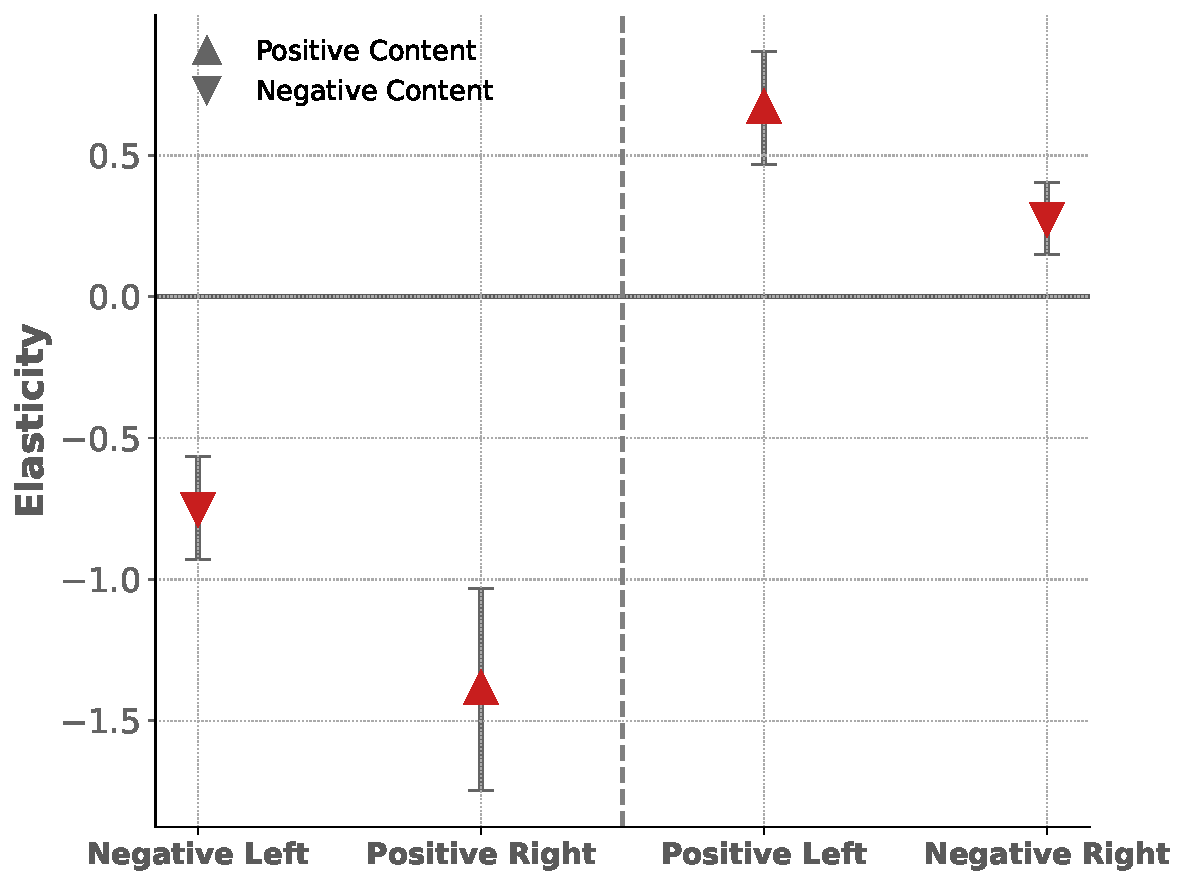
\includegraphics[width=\linewidth]{figures/elasticities_left_campaign_v4}
	 		%		\label{fig:2figsA}
	 	\end{minipage}
	 	\hfill
	 	\begin{minipage}{0.45\textwidth}
	 		\centering
	 		\vspace{1.5em}
	 		(b) Right Markets \\
	 		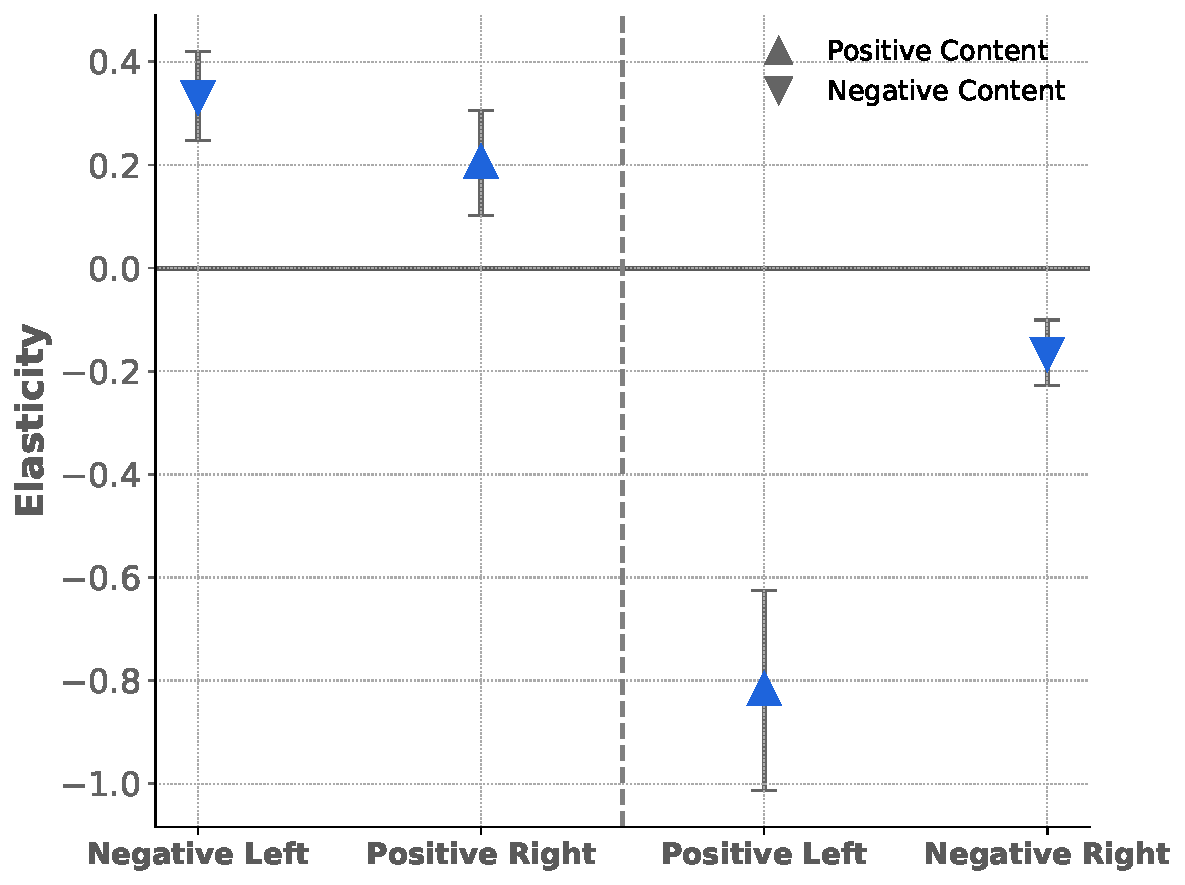
\includegraphics[width=\linewidth]{figures/elasticities_right_campaign_v4}
	 		\label{fig:2figsA}
	 	\end{minipage}
	 	
	 	\vspace{0.5em} % space between figures and note
	 	
	 	\captionsetup{justification=justified}
	 	\caption*{\small  \textit{Note:}  Each panel shows estimated mean own elasticities for consumer responses  as described in Eq. \eqref{eq:elasticities} during the campaign period. Panel (a) shows elasticities for left-leaning regions (defined as regions with below-median right-wing vote intention), and Panel (b) for right-leaning regions (above-median). Whiskers represent 95\% confidence intervals of the mean across markets.}
	 	
	 \end{figure}
	 
Furthermore, favorable partisan reactions are asymmetric across right and left markets. In-party affinity is relatively stronger in left markets (a larger reward for positive-left than for negative-right). In right markets, by contrast, out-party aversion dominates (a larger penalty for positive-left and a stronger response to negative-right). For example, a 1 p.p. increase in negative-right tone during the campaign is associated with a net loss of 8,015 viewers in right markets relative to the off-campaign period. Across both right- and left-leaning markets, audiences consistently screen out coverage that favors the opponent, and this is the content that provokes the largest reactions.

	
	
	
	

%These results are consistent with \cite{Peterson2017Echo}, who found that partisans gravitate toward like-minded political content  during the 2016 U.S. presidential campaign. Specifically, by decomposing the different-party tone combinations, I also match the \textit{affective} type of polarization, where the negative taste towards favorable content on the opposition dominates. 





\begin{comment}
content...

\begin{figure}[!htbp]
	\centering
	\caption{Estimated Elasticities for Right and Left markets, Pre-campaign and Campaign}
	
	\vspace{0.5em} % space between caption and figures
	
	\begin{minipage}{0.45\textwidth}
		\centering
		\textbf{(a)} Pre-campaign\\
		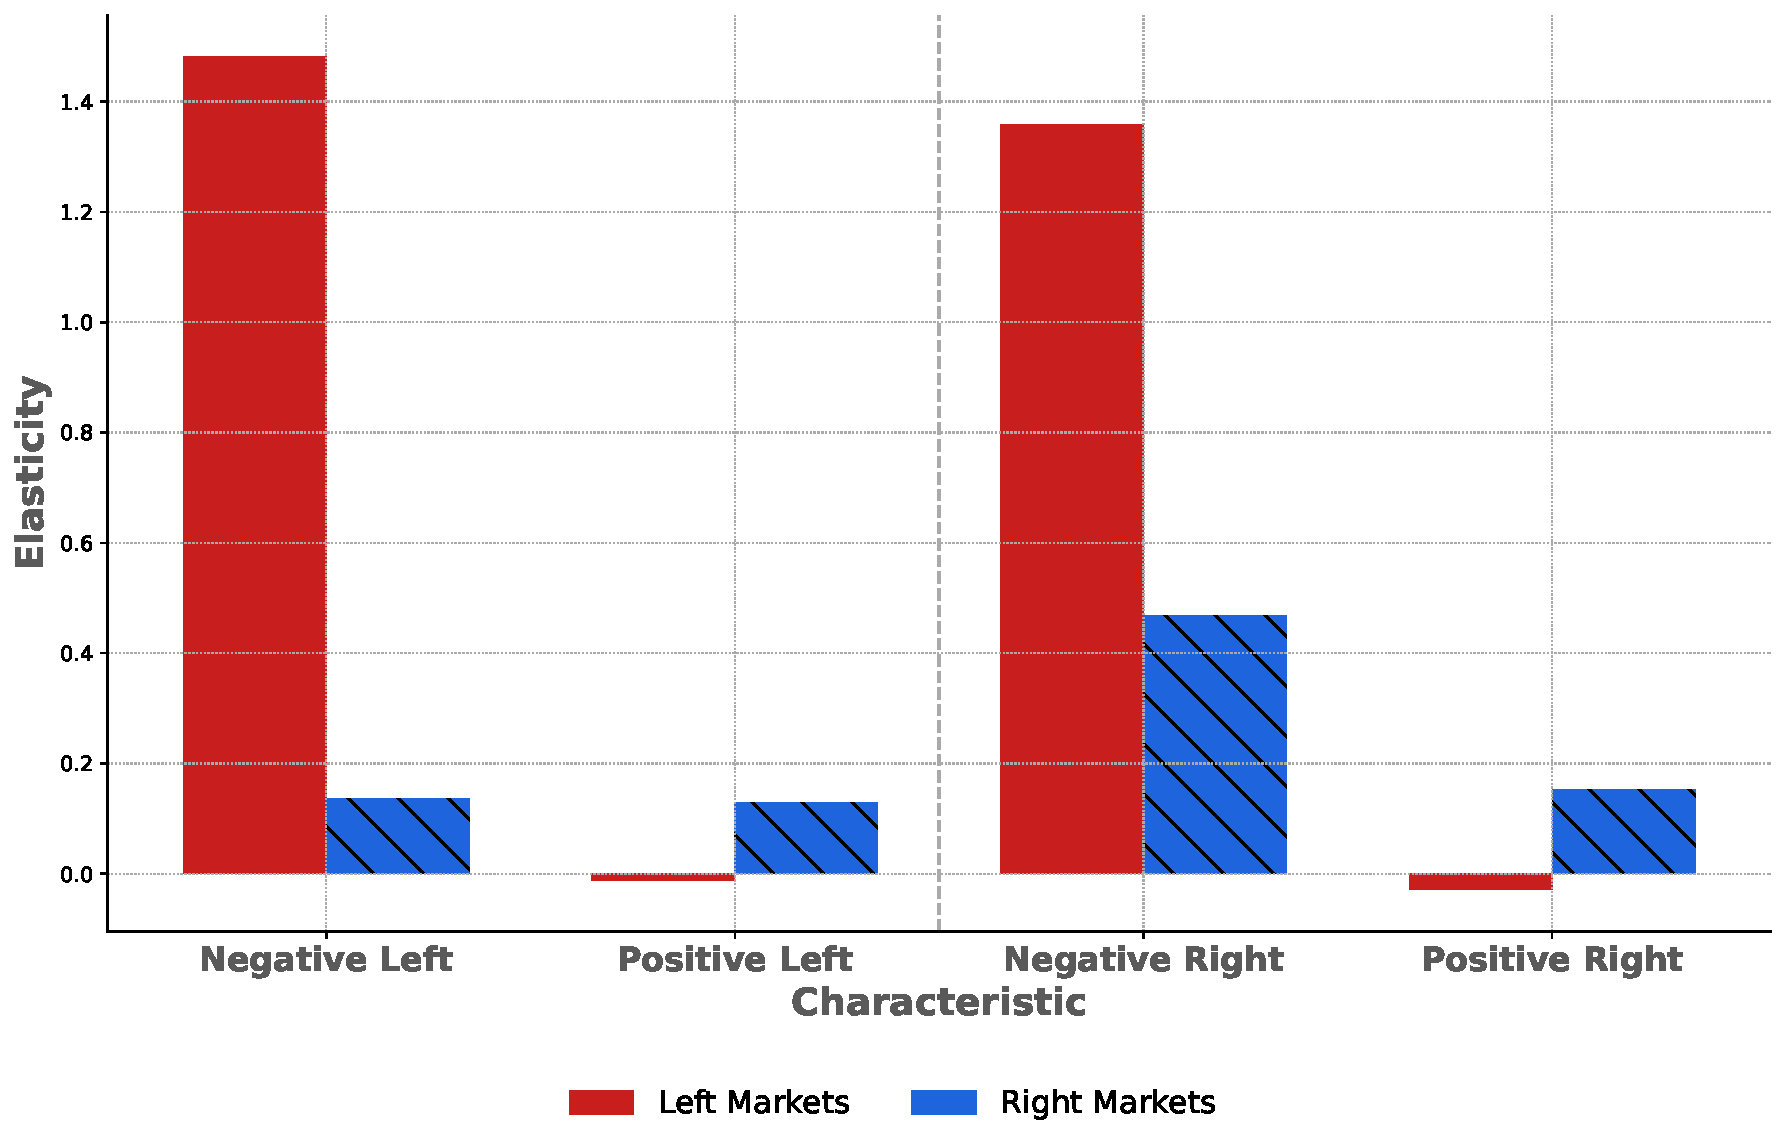
\includegraphics[width=\linewidth]{figures/elasticities_pre_campaign}
%		\label{fig:2figsA}
	\end{minipage}
	\hfill
	\begin{minipage}{0.45\textwidth}
		\centering
				\vspace{1.5em}
		\textbf{(b)} Campaign\\

		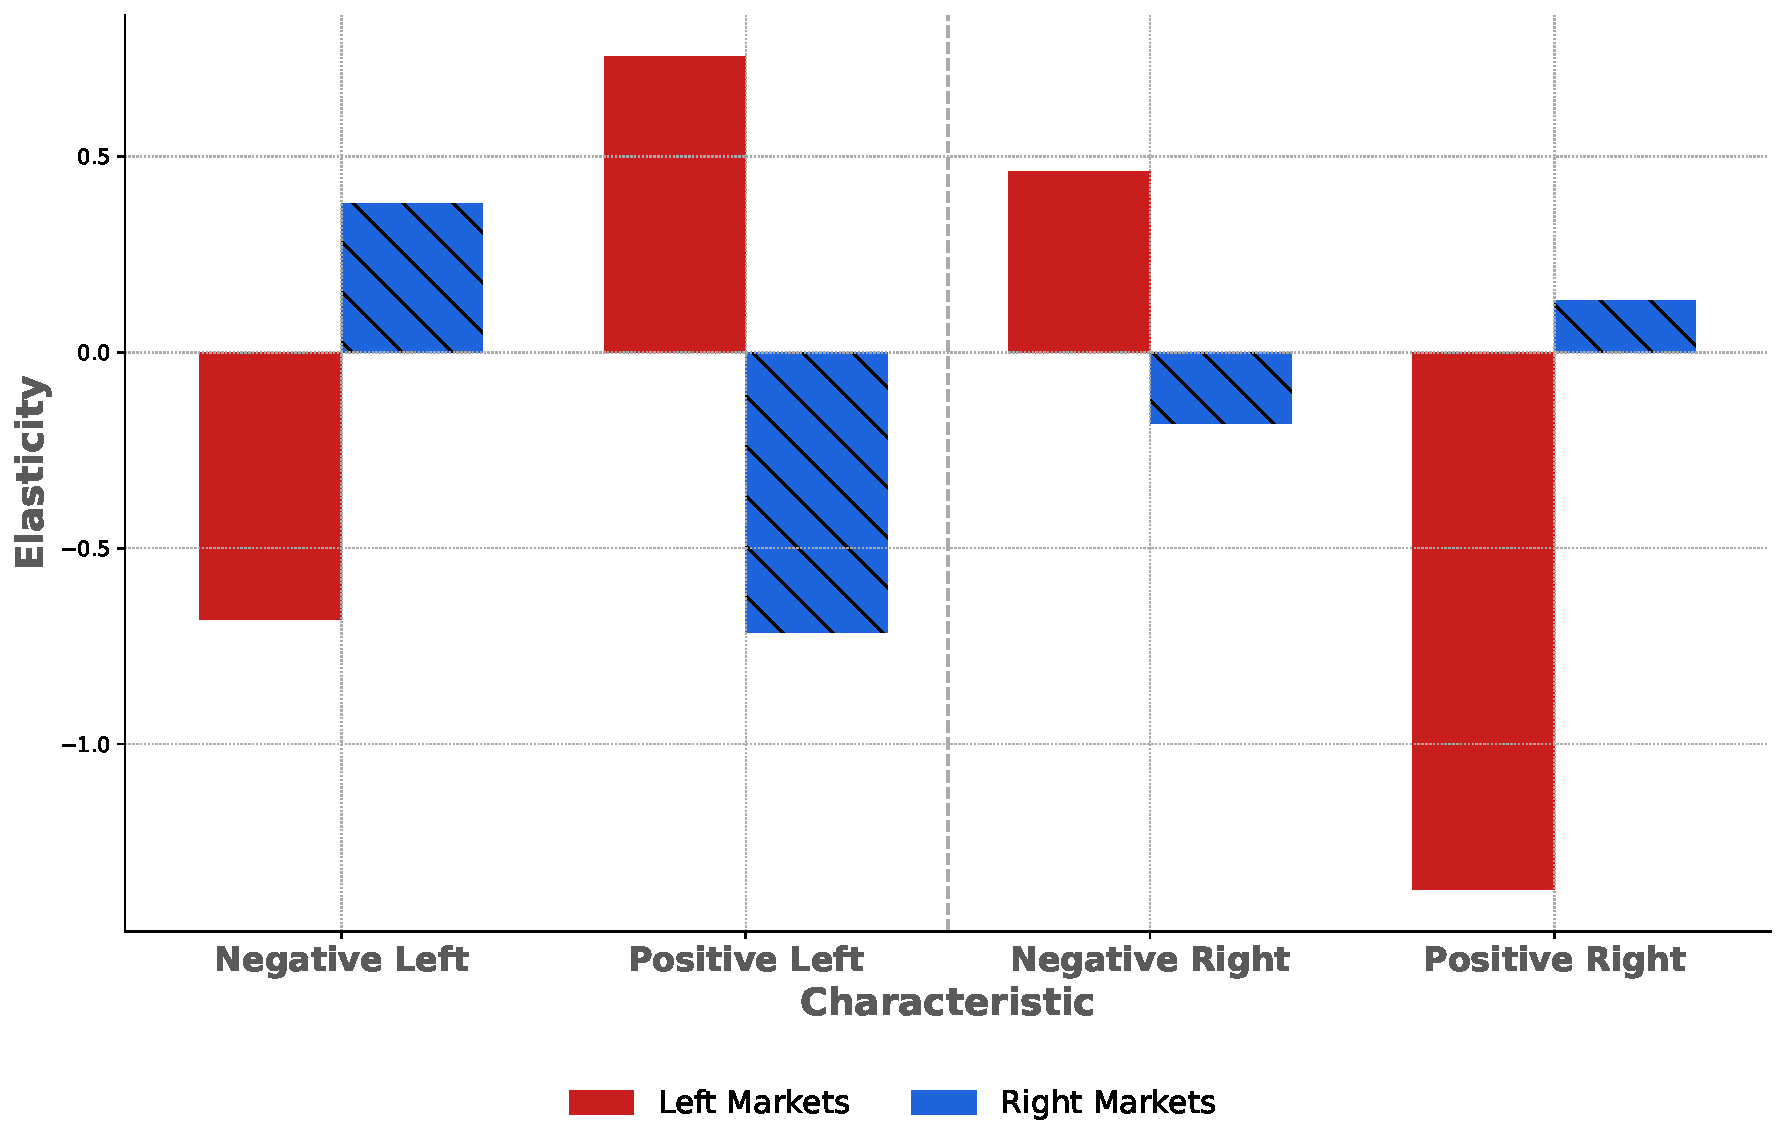
\includegraphics[width=\linewidth]{figures/elasticities_campaign}
		\label{fig:2figsA}
	\end{minipage}
	
	\vspace{0.5em} % space between figures and note
	
	\captionsetup{justification=justified}
	\caption*{\textit{Note:} \small Each panel shows estimated mean own elasticities for consumer responses in right- and left-leaning markets as described in equation \ref{eq:elasticities}. Panel (a) reports results for the pre-campaign period, while Panel (b) covers the campaign period.}
\end{figure}



\end{comment}







	\subsection{Demand for News and Electoral Polarization}
	
	
	

Does higher polarization in the demand for partisan content link to more polarized electoral attitudes?  In the spirit of \cite{martin2017}, I 
compute the Esteban–Ray (ER) polarization index and link it to the way people consume partisan news according to my demand estimates.

I compute ER on party vote intentions, which can be consistently tracked over time across survey waves  for the four main parties in my sample $\mathcal{P}=\{\mathrm{UP},\mathrm{PSOE},\mathrm{PP},\mathrm{VOX}\}$. Define $v_{prm}$ as the share of intention to vote towards party $p$ on region $r$ in month $m$; where I renormalize within $\mathcal{P}$ so that $\sum_{p\in\mathcal{P}} v_{prm}=1$. The ER index is defined as: 

\begin{equation}
	ER_{rm} \;=\; 
	\displaystyle\sum_{p\in\mathcal{P}} \sum_{q\in\mathcal{P}} 
	v_{prm}^{\,1+\alpha}\, v_{qrm}\, d_{pq},
		\label{eq:er}
\end{equation}


where $\alpha$ is set to the standard value of 1.5 and $d_{pq}$ denotes the  ideological distance between parties.\footnote{Baseline ideology scores used to compute distances: $i_{\mathrm{UP}}=-1.0$, $i_{\mathrm{PSOE}}=-0.5$, $i_{\mathrm{PP}}=0.5$, $i_{\mathrm{VOX}}=1.0$ Distances are defined as $d_{pq}=\lvert i_p-i_q\rvert/\max_{i,j}\lvert i_i-i_j\rvert \in [0,1]$.} The index $ER_{rm}$ is low when support concentrates on a single party and rises as mass is split across parties that are farther apart on the ideology scale.

	
In order to capture partisan-selective news consumption, I measure  news-demand polarization as the out-party negativity gap in audience reactions to slanted content. Specifically, I calculate the elasticity gap between reactions to congenial and uncongenial coverage during the campaign period and define \textit{media polarization} for a given region as: 
	
	
	\begin{equation}
		\textit{Media-Demand Polarization}_r  =	\begin{cases}
			\bar{\epsilon}_r^{(L-)}- \bar{\epsilon}_r^{(L+)} \quad if \quad p(r)=R\\
			\bar{\epsilon}_r^{(R-)}- \bar{\epsilon}_r^{(R+)} \quad if \quad p(r)=L
		\end{cases}
		\label{eq:mediapol}
	\end{equation}
	
	For right-wing regions ($p(r)=R$), media polarization refers to the difference in taste for negative content on the left versus positive on the left and analogously for the left-wing regions. Because the estimates satisfy
	\(\bar{\epsilon}_r^{(L-)}>\bar{\epsilon}_r^{(L+)}\) in right‑leaning regions and
	\(\bar{\epsilon}_r^{(R-)}>\bar{\epsilon}_r^{(R+)}\) in left‑leaning ones,
	the index in Eq.~\eqref{eq:mediapol} is always non‑negative and therefore comparable across regions. Higher values indicate more partisan-selective news consumption: audiences 	 respond more to negative than positive news about the party they oppose.\footnote{This interpretation aligns with in–out party evaluation gaps commonly used to capture affective polarization \citep{IyengarLelkesLevendusky2019Origins}.} I then divide regions into \textit{high} and \textit{low} groups according to their news demand polarization  relative to the median and plot their ER index for an extended period over the year before and after the 2023 election.  Results are shown in Figure \ref{fig:er1}.
	
	
	
	\begin{figure}[!ht]

		\centering
		\caption{Esteban-Ray Polarization by Level of Media Polarization}
		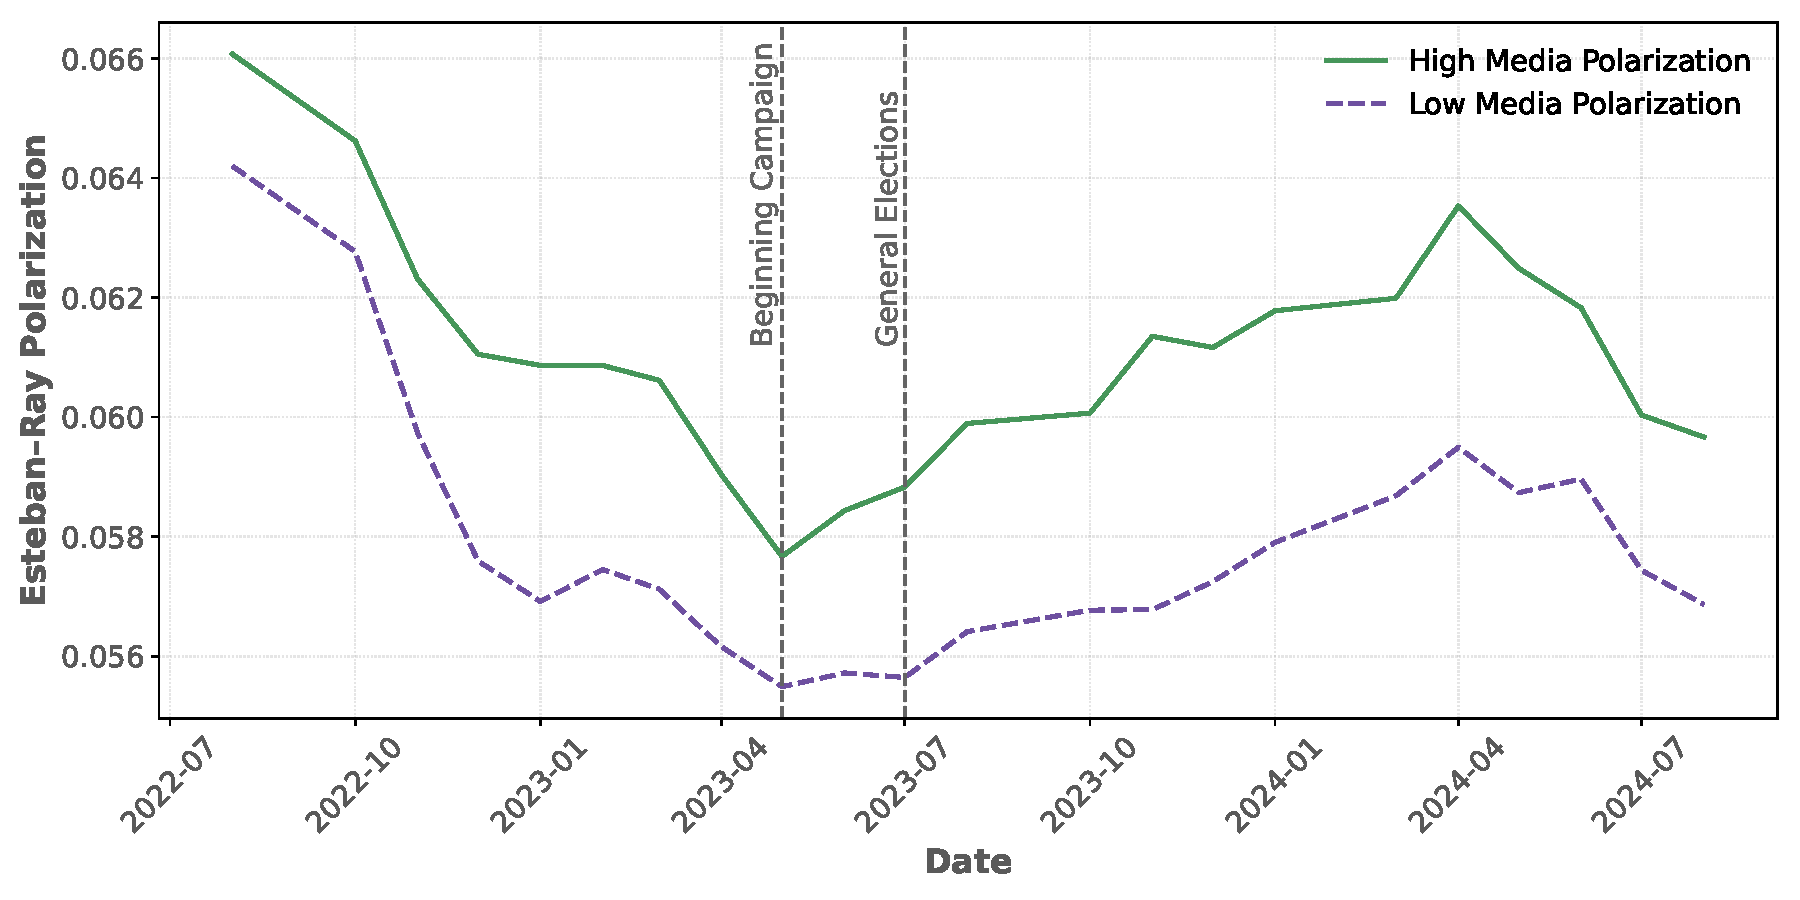
\includegraphics[width=150mm]{figures/er_polarization_stata_group_correct}
				\label{fig:er1}
		\caption*{\small  \textit{Note:} The figure shows the evolution of the Esteban–Ray polarization index as defined in Eq. \eqref{eq:er}, plotted separately for regions with high (i.e. above the median) versus low media polarization according to Eq.\eqref{eq:mediapol}. Vertical dashed lines marking the start of the campaign and election periods are shifted one to match the survey's timing.  The series covers the year before and after the 2023 general election. All series have been smoothed under a three-month centered moving average.}
		
	\end{figure}
	
	
	
Regions with high polarization in news demand (solid line) consistently show higher ER polarization; thus, consuming political information in a more partisan-selective way is associated with electorates whose vote intentions are concentrated in ideologically distant parties. Similar  to  the demand‑side results, the political campaign constitutes a structural break of one year of declining ER polarization levels  that persists for over a year. This persistence contrasts with prior work that found short-lived effects of polarization after campaigns lose salience \citep{Hernndez2020AffectivePA}. While descriptive, this pattern is consistent with persuasion mechanisms in the media literature and it motivates future work that explores the causal link between media consumption and political polarization.
	
	
	
	
%This is descriptive evidence that more partisan‑selective news consumption is associated with electorates whose vote intentions concentrate in parties farther apart ideologically.
	
	
\begin{comment}
	% ols version under the wrong ER index

Does polarization in media consumption link to electoral attitudes? I show correlational evidence between political and media polarization from my demand estimates. As in \cite{martin2017}, I compute the Esteban–Ray (ER) polarization index \citep{esteban}. Unlike \cite{martin2017}, who apply ER to a distribution of individual ideology, survey data here lack an ideology item. I therefore compute ER on \emph{two-party vote intentions} collapsed into left versus right. Formally: 

\begin{equation}
	ER_{rm}  =	 \sum_{p}   \sum_{q}
	s_{prm}^{\,1+\alpha}\,s_{qrm} \times 1,
		\label{eq:er}
\end{equation}



where  $s_{pm}$ is the share intending to vote for party $p\in\{L,R\}$ in month $m$, and I set the standard $\alpha=1.5$. With only two blocs, I normalize their distance to one. Intuitively, higher values of the  index indicate that the electorate is split into two sizeable opposing camps. In this two-party setting, ER rises precisely when when  the gap between Left and Right narrows—and it falls when one side pulls further ahead. The index is therefore a  “catching-up” indicator: low when one party dominates, highest when the two blocs are evenly matched. 

%Note that, because inter-party distance is fixed here, ER captures the balance of support across blocs (how even the split is) rather than ideological distance between them.


%where $s_{pm}$ is the share of intention to vote for party $p\in \{L,R\}$  in month $m$ and I set the standard value $\alpha=1.5$. Since there are only two blocks, the distance between political parties is normalized to one.  Higher values of the index signal a sharper left‑right split in the electorate, i.e., greater political polarization.


I measure  media polarization as the in-party vs. out-party gap in audience reactions to campaign coverage. Specifically, I calculate the \emph{elasticity gap} between reactions to congenial and uncongenial coverage during the campaign period. For right-wing regions, $p(r)=R$, media polarization refers to the difference in taste for negative content on the left versus positive and vice versa: 


\begin{equation}
	MediaPolarization_r  =	\begin{cases}
		\bar{\epsilon}_r^{(L-)}- \bar{\epsilon}_r^{(L+)} \quad if \quad p(r)=R\\
		\bar{\epsilon}_r^{(R-)}- \bar{\epsilon}_r^{(R+)} \quad if \quad p(r)=L
	\end{cases}
		\label{eq:mediapol}
\end{equation}

Because the estimates satisfy
\(\bar{\epsilon}_r^{(L-)}>\bar{\epsilon}_r^{(L+)}\) in right‑leaning regions and
\(\bar{\epsilon}_r^{(R-)}>\bar{\epsilon}_r^{(R+)}\) in left‑leaning ones,
the index in~\eqref{eq:mediapol} is always non‑negative and therefore comparable across regions. Larger values indicate that audiences penalize the out-party more (and/or reward it less) relative to the in-party, consistent with  in-out party evaluation gaps used to measure affective polarization  \citep{IyengarLelkesLevendusky2019Origins}. I divide regions into \textit{high} and \textit{low} groups according to their media polarization index relative to the median. 



Figure \ref{fig:er1} plots the ER index for these two groups over the year before and after the 2023 general election. Regions with high media‑consumption polarization (solid line) consistently show higher political polarization than their low‑polarization counterparts (dashed line)—a ranking that persists even when the series is extended one year before the main sample window. Similar  to  the demand‑side results, political polarization starts to escalate at the campaign period.


\begin{figure}[!htbp]
	
	\centering
	\caption{Political Polarization by Level of Media Polarization}
	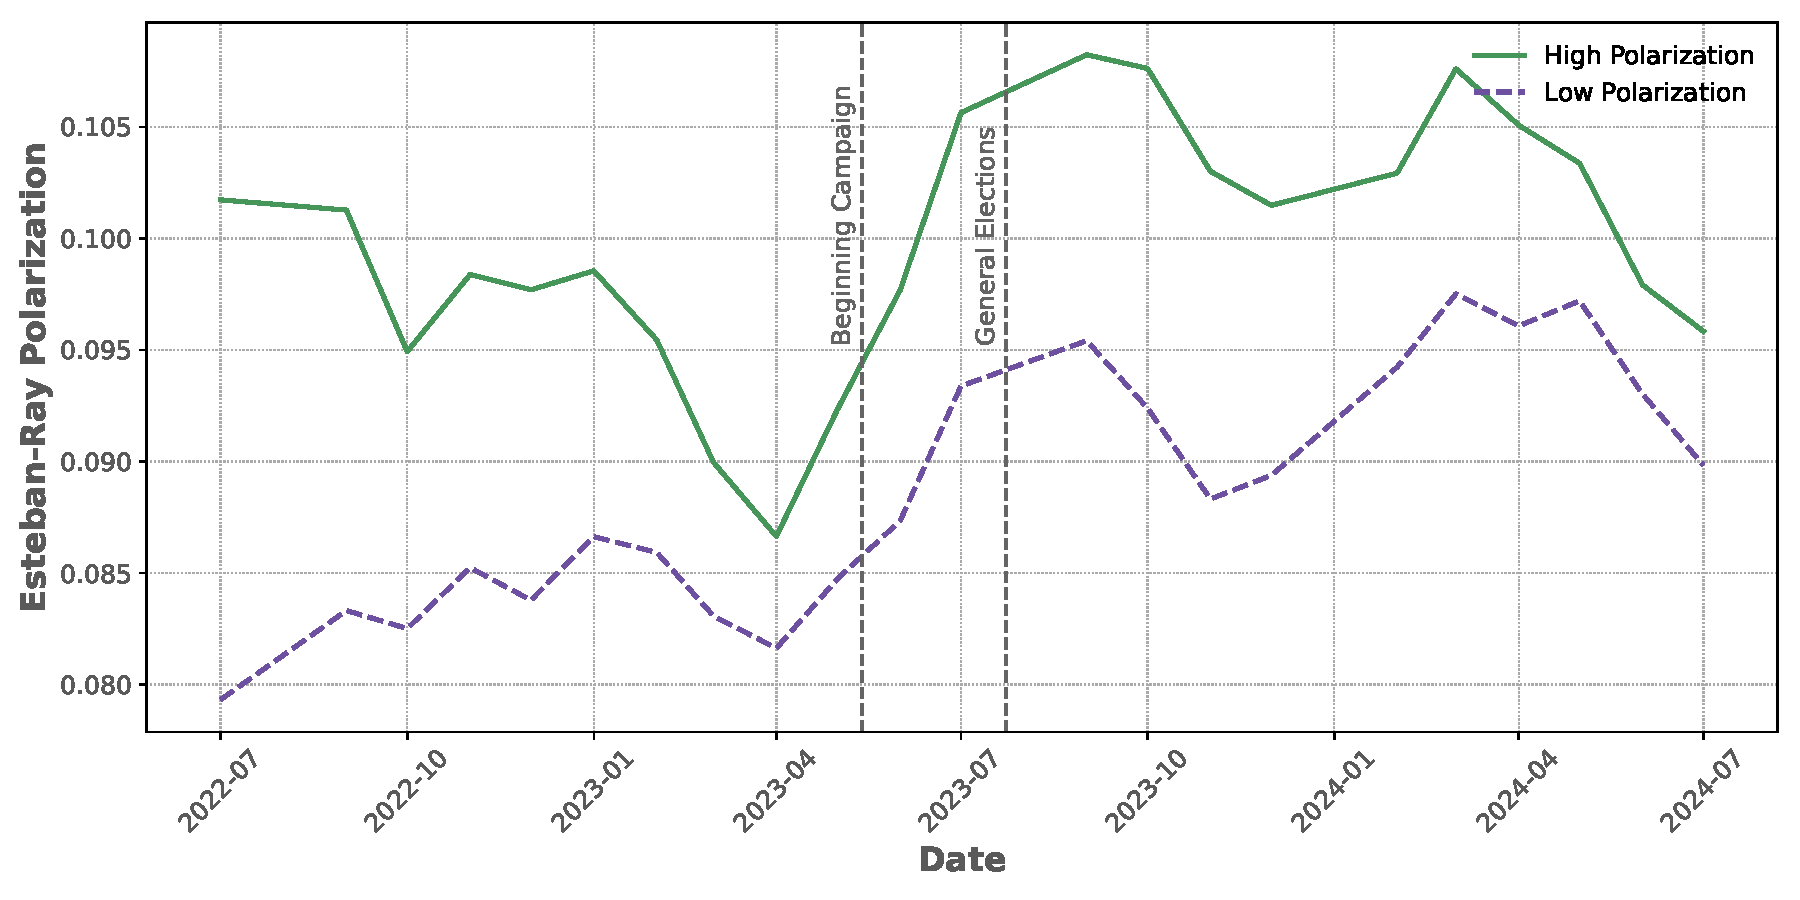
\includegraphics[width=150mm]{figures/er_polarization_stata_group}
	\label{fig:er1}
	\caption*{\small  \textit{Note:} The figure shows the Esteban–Ray polarization index of vote intentions over time, plotted separately for regions with high versus low media polarization. High-polarization regions are those above the median in the media polarization index, defined as the difference between audience reactions to out-party versus in-party coverage during the campaign (Eq. \ref{eq:mediapol}). The index is computed monthly using CIS intention-to-vote data aggregated by region. The series covers the year before and after the 2023 general election. }
	
\end{figure}

Between April 2023 and the general election in July 2023, the Esteban–Ray index rises by 0.019 points in high-polarization regions and 0.012 points in low-polarization regions. When scaled by their respective pre-campaign variability, these changes correspond to 3.8 and 5.2 standard deviations, underscoring that the campaign coincided with an unusually abrupt increase in political polarization.




%Importantly, the trend break is concentrated in high media-polarization regions—those where news consumption was already most segregated—so the observed jump in ideological polarization is essentially generated by the “extreme partisan” audiences. This pattern resonates with studies showing that selective exposure amplifies attitudes among strong partisans \citep{levendusky}, but it diverges in duration from prior work on campaign dynamics. Whereas \citet{levendusky} finds short-lived effects following exposure, and \citet{Hernndez2020AffectivePA} show that campaign-induced polarization typically reverts to baseline shortly after elections, my evidence points to a persistent shift: polarization breaks trend at the campaign’s onset and remains elevated for at least a year. A natural interpretation is that campaigns re-sort media consumption among strong partisans (reinforcement), and that this effect persists beyond the campaign window, sustaining higher polarization even after campaign salience fades. 

\end{comment}


\FloatBarrier

\paragraph{Limitations.}

To conclude the results section for demand, it is important to discuss some limitations of my analysis. 

First, the use of aggregate data cannot rule out selection effects at the individual level. Campaigns might change audience composition toward news seekers, who have been shown to have asymmetric effects on polarization relative to entertainment seekers \citep{levendusky,arceneaux_johnson_2013}. This could lead to an overestimation of preference polarization. To partly address this concern, I test compositional changes in audience based on complementary data on demographics. Appendix Table \ref{tab:compositional} shows no significant compositional differences along the age and sex dimensions from off- to on-campaign. 


Second, the link between media and political polarization naturally raises the question of how much of the shift in preferences is driven by changes in ideological polarization. I re-estimate the model in Equation~\eqref{eq:utility} using initial ideology measures (i.e., December) rather than monthly ones; the results are robust. However, this does not mitigate the concern about the potential endogeneity of ideology, which remains a limitation of this paper. Future work might address this concern using individual panel data or by allowing more flexible dynamics between ideology and media consumption, as in \cite{martin2017}.

 



\section{Supply of News}


\label{sec:supply}



The demand estimates in Section~\ref{sec:results} show that viewers react sharply to
partisan tone, especially during the campaign.  This  leads to the complementary question:
How do broadcasters decide the way they frame the news? 
The following remark from the news director of one of the channels illustrates their behavior: 


\begin{quote}
	“Even a news program is deeply subject to the day-to-day swings of audience share.  
	A drop of half a point when covering a topic can lead us to drop that topic altogether.”
\end{quote}
\hspace*{\fill}–––Vicente Vallés, Director and Presenter, A3 News (2014)\footnote{Source: \url{https://cadenaser.com/ser/2014/12/03/television/1417630810_539829.html}}

Producers therefore aim to maximize the audience shares and adapt their coverage to do so on a daily basis. In order to capture this behavior, I build a model of news slant decisions.  

\subsection{Supply Model}

Within each day's news broadcast , outlets choose the slant of the news in order to maximize national audience, but face costs of producing the slant that depend on the news pool that is available.  Formally, channel $j\in \{La \ Sexta, TVE, T5, A3\}$\footnote{Although both La Sexta and A3 belong to the same media company, AtresMedia; the short period span considered here considers them as independent products. That is, firms and products coincide. } on day $d$ and edition hour $h\in\{0\text{ (midday)},1\text{ (evening)}\}$ solves the following problem:



\begin{equation}\label{eq:payoffs}
	\begin{aligned}
		\max_{\{\mathbf{x}_{jdh}\}}   & \left\{   \sum_{r}\widehat{\bm{s}_{jrd+1}}(\bm{x}_{jdh}, \bm{x}_{-jdh})L_r -  \mathcal{C}\left(  \bm{x}_{jdh},\bm{z}_{dh}, \bm{\eta}_{jd},\bm{\nu}_{jdh}; \bm{\phi},\bm{\lambda_j}   \right)    \right\}\\
		s.t.   \quad &   x_{jdh}^{L+} +x_{jdh}^{R+} + x_{jdh}^{L-} + x_{jdh}^{R-} + x_{jdh}^{\emptyset} = x_{jdh}^{political}\\
		& x_{jdh}^k \in [0,1] \quad \forall k
	\end{aligned}
\end{equation} 



where $\bm z_{dh}$ measures the pool of stories available at edition~$h$ and $\bm x_{jdh}$ is the proportion of minutes to each tone category as defined above. $L_r$  refers to the total potential audience in region $r$. Notice that I have now incorporated the midday dimension in this analysis. The reason for this will become apparent below in the description of the identification strategy. 

The first term in the payoff captures outlets’ incentives to retain audience. Although this motive differs between the private (for-profit)  and the public broadcasters, I abstract from pricing considerations and—following \cite{Goettler2001SpatialCI}—focus on predicted audience only. This standardizes payoffs and allows the public, ad-free broadcaster to be included in the same competition game. The second term in the payoff captures the cost of producing slant as a function of the exogenous pool of stories available on a given day. I parameterize the marginal cost function of a given channel $j$ for content category $k$ as:




%\begin{equation*}\label{}
%	\begin{aligned}
	%	& \mathcal{C}(x_{jdh}^k,z_{dh}^k,\eta_{jd}^k,\nu_{jdh}^k; \bm{\phi},\lambda_j^k )\equiv  \phi_0 + \phi_1 x^k_{jdh} +   \lambda_j^k  \dfrac{(x_{jdh}^k)^2}{z_{dh}^k} + F(\eta_{jd}^k,\nu_{jdh}^k,x_{jdh}^k).
	%\end{aligned}
%\end{equation*} 

\begin{comment}
	content...

\begin{equation*}\label{}
	\begin{aligned}
		& \mathcal{C}(x_{jdh}^k,z_{dh}^k,\eta_{jd}^k,\nu_{jdh}^k; \bm{\phi},\lambda_j^k )\equiv  \phi_0 + \phi_1  \dfrac{x_{jdh}^k}{\sqrt{z_{dh}^k}} +   \lambda_j^k  \dfrac{(x_{jdh}^k)^2}{z_{dh}^k} + \beta z_{dh}^kx_{jdh}^k + F(\eta_{jd}^k,\nu_{jdh}^k,x_{jdh}^k).
	\end{aligned}
\end{equation*} 
\end{comment}

\begin{equation*}\label{}
	\begin{aligned}
		& mc(x_{jdh}^k,z_{dh}^k,\eta_{jd}^k,\nu_{jdh}^k; \phi,\lambda_j^k )\equiv   \phi +   2\lambda_j^k  \dfrac{x_{jdh}^k}{z_{dh}^k} + \eta_{jd}^k + \nu_{jdh}^k.
	\end{aligned}
	\end{equation*} 


Marginal costs depend on the ratio between the airtime share devoted to each tone category, $x_{jdh}^k$, and the share of available stories, $z_{dh}^k$. I use a flexible specification and allow the slope parameters $\bm{\lambda}_j$ that govern production costs to vary across outlets and content types. This can capture, for example, greater efficiency when journalists produce slant aligned with the outlet’s preferred ideological position. The last two components represent unobserved cost factors and are divided in: (i) $\eta_{jd}^k$, a {day-specific} marginal-cost shock (e.g., a key reporter is on sick leave, a satellite link fails, or legal review delays a segment) that is known to outlets; and (ii) $\nu_{jdh}^k$, a mean-zero, outlet–day–edition idiosyncratic supply shock that is unknown to the players.



 
 % The sign of~$\lambda_j^k$ is theoretically ambiguous ex ante. On the one hand, $z$ might act as a simple input into production costs. High availability of stories of a given type will make production easier since the journalist need not expend effort to find them. This implies $ \lambda>0$. On the other hand, since outlets are news aggregators, having more stories available of a given type might increase production costs, since outlets would need to process and filter the stories they prefer. This mechanism is consistent under $ \lambda<0$. 
 
 
 %There are unobserved (to the econometrician)  factors other than the stories available; captured by $ F(\eta_{jd}^k,\nu_{jdh}^k,x_{jdh}^k)$. The unobserved cost factors depend on two key components: i) $\eta_{jd}^k$, a \emph{ day-specific} marginal-cost shock (e.g.\ a key reporter is on sick leave, satellite link fails, or legal concerns delay a segment), and ii) $\nu_{jdh}^k$ is a mean zero channel-day-hour specific idiosyncratic supply shock. By assumption, these unobservables will enter as linear terms in the marginal costs. 
 


The first-order conditions (ignoring the  constraints for estimation) are
\begin{equation}\label{eq:focs}
	\underbrace{\sum_{r}\frac{\partial \widehat{s_{jrd+1}}}{\partial x_{jdh}^k}L_r}_{\equiv g_{jd+1h}(x_{jdh}^k)}
	= \phi + 2\lambda_j^k\frac{x_{jdh}^k}{z_{dh}^k}  
	+ \underbrace{\eta_{jd}^k+\nu_{jdh}^k}_{\equiv u_{jdh}^k}
	\quad \forall(j,k)
\end{equation}



where the derivative for all the tone characteristics also includes the marginal effect on $x^{political}$ but is omitted from the formulation for notational simplicity. The predicted audience share comes from the evening newscasts estimation but is also used to predict the midday audience share due to data limitations. This is consistent under the assumption of stable audience composition, and therefore tastes, on a given day. 



\subsection{Endogeneity and Identification Strategy}


Channels choose the day’s slant \(\mathbf{x}_{jdh}\) after observing the same-day cost shifter \(\bm\eta_{jd}\). Events like a reporter's sick leave, a technical broadcast issue or owner bias\footnote{Endogenous factors  such as outlet's private interests will be taken care of by my identification strategy if they enter linearly in the payoff specification. For instance, in the specification proposed by  \cite[][]{Anderson2010MediaMA}, owner bias would enter as a multiplicative term between owners' private ideology and the content characteristics, governed by a coefficient that captures its strength.} might shift these unobserved factors  thus affecting the optimal slant \(\mathbf{x}_{jdh}\) and thereby the demand gradient \(g_{jd+1h}(\mathbf{x}_{jdh})\).  Formally, from Equation \eqref{eq:focs},  $\E\left[\bm{u}_{jdh}\times \frac{\bm{x}_{jdh}}{\bm{z}_{dh}}\right]\neq \bm{0}$.



%Because $\eta_{jd}^k$ influences both marginal cost and the share gradient
%$g_{jd+1h}^k$ would be biased in a naive regression: $\E[g_{jd+1h}^k\,\eta_{jd}^k]\neq0$.


I exploit within-day timing for identification. The day-specific cost shock $\eta_{jd}^k$ is assumed to be realized before content production decisions and to be constant across the midday ($h=0$) and evening ($h=1$) editions. It thus captures newsroom frictions that persist throughout the day. Under this assumption, changes in chosen content between the two editions are driven by new stories arriving in the interim, $\Delta \bm{z}_d \equiv \bm{z}_{d1}-\bm{z}_{d0}$. These arrivals shift the optimal slant $\mathbf{x}_{jdh}$ by altering the marginal-cost term $\bm{x}_{jdh} / \bm{z}_{dh}$, while leaving $\bm\eta_{jd}$ unchanged.





%The key identification strategy lies in the assumption that $\eta_{jd}^k$ is constant within the day. This allows me to rely on variation in news production within the day that is only due to new stories coming in between the midday and evening editions that alter production.  


Text examples illustrate this mechanism (Table \ref{tab:within}). I filter the days with the highest within-day increase in coverage by all channels and report the new stories that entered between midday and evening editions for each content type. For instance, the biggest swing in negative-left coverage (+41 p.p.) occurred on 29 May 2023: the arrival of the overseas-ballot recount after the regional elections effectively tipped a key seat, opening a right-bloc majority, and channels incorporated those items in the evening. Analogously, on 31 May 2023 negative-right coverage rose (+22.6 p.p.) and positive-left increased (+28.2 p.p.) after afternoon legal developments unfavorable to the right and pro-government organizational updates entered between editions, shifting the evening mix the other way. These within-day arrivals of politically slanted stories are precisely the exogenous movements in content composition that I use to trace audience responses and identify $\lambda$.


%Text examples illustrate this mechanism (Table \ref{tab:within}). I filter the days with the highest within-day increase in coverage by all channels and report the new stories that entered between midday and evening editions for each content type. For instance, the biggest swing in  negative left coverage (+41pp) occured on 20 May 2023. The arrival of the ballot recount after the regional elections tipped a key seat oppening a right-bloc majority. Analogously, XXX . These within-day arrivals of politically slanted stories are precisely the exogenous movements in content composition that I use to trace audience responses and identify $\lambda$.


%On 29 May 2023, several late-day stories that were unfavorable to the left (e.g., postelection seat counts and calls for opposition coordination) entered between the midday and evening editions, shifting the overall tone toward the right. By contrast, on 31 May 2023, newly added items that were unfavorable to the right (e.g., legal and accountability developments) appeared in the afternoon and pulled the evening mix in the opposite direction; that same day, additional pieces favorable to the left (policy announcements and organizational gains) reinforced the shift. These abrupt, within-day arrivals of politically slanted stories are precisely the exogenous movements in content composition that I use to trace audience responses and identify $\lambda$.




To document this variation empirically, I first regress the evening on the midday slant of the stations controlling for outlet fixed-effects. The residuals of these regressions are the  variation in the evening programming not explained by the midday slant and channel-specific attributes. I then regress these residuals on the news shocks  that enter between those two time slots, $\Delta \bm{z}$. Figure \ref{fig:diff} shows the scatter of the regression.  The positive relationship indicates that entry of new content between midday and night is associated with an increase in editorial production of that content in the evening news shows. Unlike the pattern shown in the demand shocks,  outlets do not respond homogeneously to these arrivals (Figure \ref{fig:fwl_diff}).\footnote{To decompose this variation by outlet, I also run regressions of the form described in  \eqref{eq:first_stage} done on within-day differences $ \Delta x_{jd}$ and $\Delta z_{d}$. Although there is significantly less power now, the main mechanism still holds. Right (left) outlets increase  their production of stories of a given party-tone from midday to the evening editions conditional on those stories being aligned with their stances.} Right and left  outlets respond by increasing coverage when the content is positive, whereas they reduce the evening airtime minutes if the unexpected arrivals are negative political news. As before, asymmetries in their responses are consistent with their political positions. 


These exogenous shocks can therefore be exploited in the cost estimation to address endogeneity. Differencing~\eqref{eq:focs} eliminates the unobserved shock:

\begin{equation}\label{eq:diff_foc}
	\underbrace{%
		\sum_{r}\left(
		\frac{\partial \widehat{s_{jrd+1}}}{\partial x_{jd1}^k}
		-
		\frac{\partial \widehat{s_{jrd+1}}}{\partial x_{jd0}^k}
		\right)L_r
	}_{\textstyle \Delta g_{jd+1}^k}
	\;=\;
	2\lambda_j^k
\Delta\left( \frac{x_{jd}^k }{z_{d}^k } \right)
	\;+\;
	\Delta\nu_{jd}^k,
	\quad \forall (j,k).
\end{equation}



 Intuitively, the evening–midday change in the gradient, $\Delta g_{jd+1}^k$, is driven by the change in story availability $\Delta	
\frac{x_{jd}^k }{z_{d}^k }$, while the day-persistent cost shock cancels out. The system of equations in \eqref{eq:focs} can be estimated under GMM with conditions $\E \left[\Delta  \left( \frac{\bm{x}_{jd}}{\bm{z}_{d}} \right)  \Delta\bm\nu_{jd} \right]= \bm{0} $. 




Notice that the parameters $\left(\phi,\bm\eta \right)$ cancel out in the differentiation and thus cannot be identified but they are part of the overall cost and thus needed to interpret them. They can be recovered by rearranging from the   first-order condition in \eqref{eq:focs}. De fine the residual as:

\[
r_{jdh}^k \;\equiv\;\phi+\eta_{jd}^k+ \nu_{jdh}^k= {{g}_{jd+1h}} \;-\; 2\,{{\lambda}}_j^k\,\frac{x_{jdh}^k}{z_{dh}^k}.
\]


Since $\E(\nu_{jdh}^k)=0$, an unbiased estimate of the unobserved marginal cost shifter $\bm\eta + \phi$ is obtained by averaging across the midday and evening editions of $r_{jdh}$,


\[
\widehat{\phi +\eta_{jd}^k} = \tfrac{1}{2}\big(\hat{r}_{jd0}^k+\hat{r}_{jd1}^k\big).
\]


In the counterfactual problem \eqref{eq:payoffs2}, I treat this estimate  as given (fixed by day and channel) and solve for best responses under the policy constraints, so changes arise from the policy, not from altering day-specific costs.



\subsection{Results of the Supply Estimation}

 The sign of~$\lambda_j^k$ is theoretically ambiguous ex ante. If, as suggested in \cite{SimonovRao2022}, high availability of stories of a given type will make production easier since the journalist need not expend effort to investigate,  $z$ might act as a simple input into production costs and $ \lambda>0$. On the other hand, since outlets are news aggregators, having more stories available of a given type might increase production costs, since they would need to process and filter the stories they prefer. This mechanism is consistent under $ \lambda<0$. I therefore do not restrict the $\lambda$ to be positive in the estimation and show robustness under stricter version of $\lambda \geq0$.


Table~\ref{tab:costs} reports the estimated $\lambda_j^k$.\footnote{Processing of the midday broadcasts for the pre‑campaign period could not be completed after the Google Cloud and OpenAI credits ended; consequently, the cost estimates here cover only the campaign window. } There is heterogeneity both  across outlets and content types, and it partly lines up with editorial positions. For instance, left outlets face higher costs for negative-left content, whereas the right-leaning channel does not. Producing content that favors the right is intrinsically beneficial across outlets ($\lambda<0$), but especially so for right channel. Negative-right content is beneficial or less costly for left outlets, while A3 faces the highest cost in that category. The main deviation from this pattern is positive-left content, where signs match with the negative left one and thus do not reflect the expected asymmetries. 


%Producing content favorable to the left (positive-Left or negative-Right)
%is costlier for the right-leaning A3,
%while the reverse holds for left-leaning La~Sexta and TVE.  
%T5, a centrist outlet, faces the lowest absolute costs in every category.



\begin{comment}
\begin{table}[!htbp]
	\caption{Estimated Cost Parameters ($\lambda$) by Channel and Content Type}
	\label{tab:costs}
	\centering\small
	\begin{tabular}{lcccc}
		\toprule
		& La~Sexta & TVE & Telecinco (T5) & Antena~3 (A3)\\
	& 	\scriptsize{(Left)} & \scriptsize{(Left)} & \scriptsize{(Middle)}& \scriptsize(Right) \\
		\midrule
		% Group 1
		Negative Left   
		& 12.782   &  6.614   & 108.985   & --38.135  \\
		& (44.512) & (3.107)  & (60.695)  & (24.006)  \\
				\midrule
		Positive Right  
		& --89.175 & --105.658 & --13.868  & --238.018 \\
		& (85.860) & (121.713) & (91.624)  & (77.314)  \\
		\midrule
		% Group 2
		Positive Left   
		& 36.094   &  3.368   &  25.984   & --38.962  \\
		& (52.716) & (13.110) & (43.586)  & (84.390)  \\
				\midrule
		Negative Right  
		&  4.059   & --8.694  &  30.280   &  34.624   \\
		& (4.788)  & (11.057) & (36.013)  & (53.835)  \\
		\midrule
		% Group 3
		Political 
		& --0.349  &  0.317   &   1.498   &   1.455   \\
		& (0.610)  & (0.622)  &  (1.049)  &  (1.248)  \\
		\bottomrule
	\end{tabular}
	\vspace{0.5em}
	\caption*{\small \emph{Note:} Robust standard errors in parentheses. The table shows the estimated coefficients from the unconstrained GMM for the system in Equation \ref{eq:diff_foc} for the campaign period.}
\end{table}
\end{comment}



\begin{table}[!htbp]
	\caption{Estimated Cost Parameters ($\lambda$) by Channel and Content Type}
	\label{tab:costs}
	\centering\small
	\begin{tabular}{lcccc}
		\toprule
		& La~Sexta & TVE & Telecinco (T5) & Antena~3 (A3)\\
		& \scriptsize{(Left)} & \scriptsize{(Left)} & \scriptsize{(Middle)} & \scriptsize{(Right)}\\
		\midrule
		Negative Left & 12.82 & 6.27 & 108.34 & -38.96 \\
		& (44.44) & (2.63) & (60.39) & (23.79) \\
		\midrule
		Positive Right & -89.09 & -103.74 & -13.87 & -240.52 \\
		& (85.99) & (121.36) & (91.62) & (77.50) \\
		\midrule
		Positive Left & 36.11 & 3.36 & 24.03 & -40.03 \\
		& (52.70) & (13.12) & (43.99) & (84.81) \\
		\midrule
		Negative Right & 4.07 & -8.88 & 31.13 & 35.16 \\
		& (4.80) & (11.41) & (36.16) & (53.89) \\
		\midrule
		Political & -0.35 & 0.32 & 1.50 & 1.45 \\
		& (0.61) & (0.62) & (1.05) & (1.25) \\
		\midrule
		\bottomrule
	\end{tabular}
	\vspace{0.5em}
	\caption*{\small \emph{Note:} The table shows the estimated coefficients from the unconstrained GMM for the system in Equation \eqref{eq:diff_foc} for the campaign period. Robust standard errors in parentheses. }
\end{table}








%the heterogeneity in the estimated coefficients partly aligns with outlet's slant positions. Producing negative content on the left is costlier for all but the right wing channel. 




%The signs confirm the interpretation: left-favorable content is costlier for right-leaning outlets, and vice versa for all characteristics but  positive left content. It is important to remark that the interpretation of these cost parameters is broad and cannot be disentangled into different factors. Higher values of $\lambda$ could reflect costs in the production of certain content due to specialization of the journalists, having less access to information sources and/or private interests. 

%To give a size effect, costs are expressed in thousands of viewers and can be interpreted in terms of audience shares. Increasing a 1pp increase in positive left tone from their baseline medians is 0.08 share points more costly than negative left tone for the right wing channel A3 and only 0.03 for the left outlets. Increasing 1pp in positive tone of the right is 0.06 share points less costly than negative right for the right outlet and 0.01 shre points more costly than negative for the negative outlets. 


Costs are measured in thousands of viewers and map directly into audience values, so they can be read as “how much audience a channel gives up” to shift tone. A 1 p.p. increase (from the median) in positive coverage of the left is relatively expensive for the right-leaning channel A3: it costs 8 p.p. of audience share  more than moving the same amount toward negative coverage of the left. For left-leaning outlets, the same shift is far smaller, only 3 p.p. more than going negative. In contrast, a 1 p.p. increase in positive coverage of the right is 6 p.p. less costly than going negative for the right-leaning outlet, while for left-leaning outlets it is 1 p.p. more costly than going negative. 



Given the demand and supply estimates, I recover the total payoffs for each outlet and tone.  Figure \ref{fig:payoffs} plots the payoff functions (in thousands of viewers). Figure \ref{fig:payoffs_constrained} shows the payoffs under the non-negativity constraint. The ranking of payoffs is stable across the two specifications. For both parties, negative-tone categories dominate: the right-leaning channel obtains a maximum of  around 500 thousand viewers with negative-left content (vs. ~400 thousand at the maximum positive-left tone), while the left-leaning outlets get a maximum of around 300 thousand with negative-right content (vs. ~90 thousand with positive-right).

%The right-leaning outlet enjoys higher payoffs for producing positive-right content and negative-left content, whereas the left-leaning outlets obtain higher payoffs for negative-right content. The only inconsistency arises in the positive-left category, where the right-leaning outlet’s payoff is strictly increasing; this pattern reflects the cost parameters for this category reported in Table \ref{tab:costs}. 






%\paragraph{Limitations}
%The supply estimation carries a number of limitations. First, broadcasting content nationally leaves days as the only source of independent variation to exploit, reducing sample size and statistical power. This is reflected in the very imprecise estimates in Table~\ref{tab:costs}. Second, parameterizing the cost function requires assumptions on functional form. The quadratic specification used here imposes marginal cost linear in $x$ and allows to exploit its within day variation for identification, but other functional forms could also be consistent with the competition game.



%Given the demand and supply estimates, in the next section I present the counterfactual analysis testing policy regulations on content. 




\FloatBarrier










\section{Proportional Air Time Rule}

\label{sec:counter}


Across Europe, election coverage is commonly regulated by proportional-time rules tied to party representativeness. In France, for instance, the broadcast regulator ARCOM monitors  the speaking time and airtime of political actors in news bulletins, news magazines and other programs on TV and radio to enforce political pluralism. During campaigns these rules apply to all programs covering the election. ARCOM requires equitable coverage (proportional to representativeness) and, in the presidential election, strict equality of speaking time and airtime from the start of the official campaign. In Italy, the communications authority AGCOM enforces the par condicio law, which governs access to programs of information and political communication on television and radio. During electoral periods, AGCOM requires that news and political programs allocate speaking and news time proportionally to each party’s representativeness. These rules apply explicitly to news bulletins and current-affairs programs.\footnote{More details about the regulations can be checked at  \href{https://www.arcom.fr/nous-connaitre-nos-missions/garantir-le-pluralisme-et-la-cohesion-sociale/proteger-le-pluralisme-politique}{https://www.arcom.fr/nous-connaitre-nos-missions/garantir-le-pluralisme-et-la-cohesion-sociale/proteger-le-pluralisme-politique} for ARCOM and at \href{https://www.agcom.it/sites/default/files/migration/delibera/Delibera\%20122-24-CONS.pdf}{https://www.agcom.it/sites/default/files/migration/delibera/Delibera\%20122-24-CONS.pdf} for AGCOM. }
%In France and Italy, the broadcast regulators (\textit{ARCOM} and \textit{AGCOM}) require proportional allocation of coverage during official campaign periods. Spain, by contrast,  does not have a media-pluralism authority and lacks any enforced regulation. 





%Across Europe, the most common rule for election coverage is proportional airtime. France’s ARCOM times every political segment and enforces near  balance during the official campaign for both public and private broadcasters. Similarly, Germany or Italy's \textit{Par Condicio} tie lengths to past vote shares. Spain, by constrast, remains unregulated. 

My model estimates allow me to assess the  implications of the proportional-airtime rule for all broadcasters.  I take the proportion of votes in the past general elections for each party ($vote^R,vote^L$) and estimate the new equilibrium under the following problem: 




\begin{equation}\label{eq:payoffs2}
	\begin{aligned}
		\max_{\{\bm{x}_{jd}\}}   & \left\{   \sum_{r}\widehat{s_{jrd+1}}(\bm{x}_{jd}, \bm{x}_{-jd})L_r - \sum_k \left({\hat{\lambda}_j^k}  \dfrac{(x_{jd}^k)^2}{z_{d}^k} + \widehat{\left(\phi+{\eta}_{jd}^k\right)} x_{jd}^k \right)  \right\}\\
		s.t.   \quad &   \frac{x_{jd}^{R+} + x_{jd}^{R-} }{x_{jd}^{political}}=vote^R\equiv0.51\\
		&  \frac{x_{jd}^{L+} + x_{jd}^{L-} }{x_{jd}^{political}}= vote^L\equiv0.49\\
       &  x_{jd}^{L+} +x_{jd}^{R+} + x_{jd}^{L-} + x_{jd}^{R-} \leq  x_{jd}^{political}\\
		& x_{jd}^k \in [0,1] \quad \forall k
	\end{aligned}
\end{equation} 


where, in a logic consistent with my measurement strategy, time to a political party can only be discerned if that story has some specific slant. I assume that the policy is enforced; that is, all outlets must devote the proportion of political time given by vote shares from the previous election $(vote^R, vote^L)$ (i.e, constraints bind). This simplifies the choice set to $\left( x_{jd}^{L+} ,x_{jd}^{R+} ,x_{jd}^{political}\right)$. For computational constraints I i) pool left channels as a single player using their average payoffs and ii) discretize the action space and solve for the pure Nash equilibrium after converting the problem into a normal form game.\footnote{ In the original normal form game, the joint action space consists of 	$20^4=160,000$  pure strategy profiles under the simplest grid of 3 points per action. The counterfactual constraints simplify the action space to $4,096$ strategy profiles.  The code was run under a Google Cloud “n2d-standard-224” virtual machine (224 vCPUs, 896 GB RAM).} 

%Another important assumption in the counterfactual analysis relates to the unobserved marginal cost shifters $\eta$ in equation \ref{eq:focs}. Since the $\lambda$ parameters were estimating by first differencing and the small sample size does not leave enough degrees of freedom to estimate $\eta_{jd}^k$ as fixed effects, these terms are not included in the cost function in the counterfactual game in \ref{eq:payoffs2} (i.e I assume $\bm{\eta}= \bm{0}$).


%From the  first-order condition in \eqref{eq:focs}, define the error

%\[
%r_{jdh}^k \;\equiv\; {{g}_{jd+1}} \;- \phi_1-\; 2\,{{\lambda}}_j^k\,\frac{x_{jdh}^k}{z_{dh}^k}
%\;=\; \eta_{jd}^k + \nu_{jdh}^k ,
%\]



\subsection{Effects of the Regulation}

Results of the counterfactual estimation are shown in Table \ref{tab:counter}.  The left columns report the baseline, average minutes for each category during the campaign and the right column reports the results from the counterfactual equilibrium. 



\begin{table}[!htbp]
	\caption{Baseline and Counterfactual Slant by Channel}
	\label{tab:counter}
	\centering\small
	\begin{tabular}{lcccccc}
		\toprule
		& \multicolumn{2}{c}{La~Sexta/TVE} & \multicolumn{2}{c}{Telecinco (T5)} & \multicolumn{2}{c}{Antena~3 (A3)} \\
		& \multicolumn{2}{c}{(Left)} & \multicolumn{2}{c}{(Middle)} & \multicolumn{2}{c}{(Right)} \\
		& Baseline & Count. & Baseline & Count. & Baseline & Count. \\
		\midrule
		Negative Left & 0.06 & 0.05 & 0.04 & 0.36 & 0.09 & 0.45 \\
		\midrule
		Positive Right & 0.03 & 0.00 & 0.03 & 0.00 & 0.04 & 0.01 \\
		\midrule
		Positive Left & 0.09 & 0.10 & 0.04 & 0.10 & 0.06 & 0.01 \\
		\midrule
		Negative Right & 0.09 & 0.15 & 0.04 & 0.44 & 0.07 & 0.43 \\
		\midrule
		Political & 0.42 & 0.30 & 0.18 & 0.90 & 0.39 & 0.90 \\
		\midrule
		\bottomrule
	\end{tabular}
	\vspace{0.5em}
	\caption*{\small \emph{Note:} The table reports the average share of minutes per category. Baseline values refer to observed campaign broadcasts; counterfactual values are predicted from solving from solving the counterfactual optimization problem in Equation~\eqref{eq:payoffs2}.      Channels are grouped as: left-leaning (La~Sexta, TVE), middle (T5), and right-leaning (A3).}
\end{table}


%Several facts emerge from the counterfactual exercise. First, left-leaning outlets (La Sexta/TVE) reduce the overall share of political coverage from 42\% to 30\% when constrained to allocate airtime proportionally. Since they are forced to spend more time on right-wing coverage, they cut back on politics altogether and shift  toward a more negative tone of the right (from 0.09 to 0.15). At the same time, their positive coverage of the left remains broadly unchanged, implying that compliance is achieved primarily by eliminating right-positive content and compensating with hostile tone.


%Second, the centrist outlet (T5) responds by dramatically expanding its political content, from 18\% of airtime in the baseline to 90\% in the counterfactual. The strong responses on politics can be explained by the combination of supply and demand parameters. With low marginal costs of producing politics ( Table \ref{tab:costs}), optimal political share $x^{political}$ will mainly be driven by demand tastes. From the demand estimation results (Table \ref{tab:results_blp}), right-(left-)wing viewers demand positive (negative) amount of political content. The combination of cheap politics on the cost side and strong campaign-period demand asymmetries on the viewer side thus delivers the large increases (decreases) in political airtime for  right- and left-wing outlets in the counterfactual. 


Several facts emerge from the counterfactual exercise. First, in terms of political coverage, the left-leaning outlets slightly reduce it, whereas the middle (T5) and right (A3) sharply increase it to 90 percent. These responses are consistent with the model’s supply and demand estimates. With low marginal costs of producing political content (Table~\ref{tab:costs}), the optimal political share, $x^{\text{political}}$, is mainly driven by viewer preferences. From the demand estimates (Table~\ref{tab:results_blp}), right-wing viewers value political content positively, while left-wing viewers value it negatively. This makes it profitable for the right-leaning outlet to expand political minutes, though less so for outlets with left-leaning audiences. Second, the increase in political content comes almost entirely in the form of negative tone of the opposing party. The right-leaning outlet increases negative coverage equally for both parties and the left-leaning outlets do so only for the right. The "negativity" in the equilibrium is consistent with the payoffs shown in Figure \ref{fig:payoffs}, where each outlet enjoys significantly more viewers from raising negative rather than positive tone on the opposed. 



Taken together, these adjustments generate a  more polarized landscape. Figure \ref{fig:change_line_counter} illustrates the resulting shifts in outlets’ ideological positions: left-leaning and centrist outlets move further left, while A3 strengthens its rightward tilt. Importantly, the regulation compresses the space for balanced coverage by regulating political airtime but leaving tone unconstrained. Dispersion across channels' slant positions increased from 0.06 to 0.20, leading to a much more polarized media environment.
%with a notable rise in the standard deviation from 0.03 to 0.1, 

Evaluating demand at the counterfactual equilibrium shows that, naturally, since content offered is more partisan, the effects on overall viewership escalates with it.  In right-leaning regions, a 1 p.p. increase in net right tone attracts on the order of 60 thousand more viewers more than the baseline. Similar, symmetric responses occur in  left-leaning markets.\footnote{Table \ref{tab:elasticities_count} shows the estimated elasticities for both the Baseline and Counterfactual estimations. } Fixing airtime while leaving tone unconstrained therefore first makes outlets go more negative and then amplifies affective polarization on the demand for political content. 



To sum up, enforcing proportional-airtime constraints raises slant dispersion by pushing outlets toward more negative tone. Given polarized viewing preferences, this amplifies polarization in media demand. These patterns are especially worrisome since recent evidence shows that more negative campaign content increases affective polarization and selective exposure \citep{lau2017effect}.




\paragraph{Limitations} Finally, the counterfactual results should be interpreted with caution. First, as noted before, I discretize each outlet’s action space on a coarse grid; best responses can be pushed to grid boundaries, yielding corner solutions that may over- or understate the continuous-choice equilibrium. Second, I retain only equilibria for which a unique pure-strategy Nash equilibrium is found. This excludes realizations with multiple (or mixed-strategy) equilibria and may bias inference toward stability. If multiplicity matters, equilibrium selection could depend on unmodeled factors. Third, for tractability I pool La Sexta and TVE into a single left player with averaged payoffs. This removes within-bloc competition and coordination frictions; in the full four-player game, left outlets might either undercut one another on tone or differentiate strategically, altering the comparative statics. Relaxing these assumptions could dampen or reshape the effects.



	
	\section{Conclusion}
	\label{sec:conclusion}
	

This paper studies how election campaigns reshape demand for political news using a structural model of news demand and supply. I construct a story-level slant index for Spanish prime-time TV newscasts by combining machine learning with large language models (LLMs) and match it to high-frequency audience-meter data. This allows me to track, over time, both the partisan tone to which viewers are exposed and their viewing responses.



%On the demand side, I estimate a BLP-style random-coefficients model where viewers choose their preferred channel to consume news based on the way outlets treat political content. Since content is an equilibrium outcome, and thus endogenous, I propose an identification strategy that relies on supply shocks that constrain outlets’ ability to slant the daily news, which varies with the random composition of available events. I find a significant change in how political news is consumed: during the election campaign, viewers polarize their news consumption, screening out favorable content about the opposing party and favoring their own. This polarization in the demand for political content is also associated with higher and more persistent political polarization in the electorate. On the supply side, the estimated cost parameters show substantial heterogeneity in the cost of producing slant, aligned with each outlet’s ideological stance.


On the demand side, I estimate a BLP-style random-coefficients model in which viewers choose a channel based on how outlets treat political content. Since content is chosen by outlets in equilibrium, it is endogenous. In order to identify demand preferences I rely on supply shocks that come from day-to-day changes in the available stories and limit how much outlets can slant the news. During the campaign, viewers polarize their consumption of political news, screening out coverage favorable to the opposing party and favoring their own. This pattern in news demand is also associated with higher and more persistent polarization in the electorate. On the supply side, the estimated cost parameters show substantial heterogeneity in the cost of producing slant, aligned with each outlet’s ideological stance.


Building on the demand and supply estimates, I evaluate the effects of  proportional-airtime rules on broadcasters during campaigns. The counterfactual results show that, while channels deliver balanced airtime across parties, this masks an increase in the polarization of the slant they supply. The mechanism follows from the rule’s design: because only total exposure in minutes is constrained, outlets comply by adjusting tone, which widens cross-outlet dispersion in supplied slant and strengthens audience responses to partisan content.

This paper highlights two main points. First, surges in ideological polarization during political conflict are mirrored in how voters consume news: campaigns do not just inform, they reshape information preferences and can amplify affective polarization. Second, widely used metrics for monitoring media bias—such as airtime balance—overlook tone, which can lead to poorly targeted interventions. The  framework developed in this work provides a more robust basis for media monitoring and a path for evaluating regulatory measures.



Several avenues for future research emerge from the present work. Leveraging the unique feature of the dataset—which allows to compare the tone and coverage of the same story across outlets on a given date—future work could micro-found editorial decisions  to distinguish between different forms of bias, such as distortion or filtering as theorized in previous works \citep[e.g.][]{gentzkow2014media}. Another promising direction is to study the role of newswire agencies as  upstream providers of information.  Because these services are broadly accessible across countries, the same benchmark can be applied in both democracies and autocracies to estimate media bias and analyze polarization in news demand.







	
	%On the demand side, I estimate a BLP-style random-coefficients model identified using exogenous variation in the daily story mix available to outlets. Consumption polarizes sharply during the campaign, in a way consistent with affective polarization: viewers penalize negative news about their own political side and, in particular, discount content favorable to the opposing party. I then document a positive association between media-demand polarization and survey-based electoral polarization of vote intentions. Given the demand estimates, I model the supply of information as a competition game in which outlets choose the slant of their programs to maximize audience, incurring tilting costs that depend on the pool of stories available each day. The cost estimates are consistent with heterogeneity in slant production, with right- (left-) leaning outlets facing higher costs of producing uncongenial content.
	
	
	
	
	
	
	
	%\nocite{*}
	\clearpage
	%\addcontentsline{toc}{chapter}{Bibliography}
	%\printbibliography
	
	%\addcontentsline{toc}{chapter}{Bibliography}
	\pagestyle{plain}  
	\bibliographystyle{apa}
		\bibliography{./bib/media_bias.bib}
	
	
	
	\clearpage

\appendix

\addcontentsline{toc}{section}{Appendix} % Add the appendix text to the document TOC
\part{Appendix} % Start the appendix part

\parttoc % Insert the appendix TOC


\renewcommand\thefigure{\thesection.\arabic{figure}}   
\renewcommand\thetable{\thesection.\arabic{table}}
\setcounter{table}{0}


\clearpage






\section{Data Pipeline  Details}\label{sec:appendix_models}



This appendix describes the end-to-end pipeline used to collect, process, and analyze Spanish prime time newscasts. The workflow follows  Figure~\ref{fig:pipeline}: daily recordings are stored, audio is extracted and transcribed, text is segmented into minute-level stories, topics are estimated with a topic model, and political tone is classified with a large language model. The corpus comprises the midday and evening national newscasts of TVE, A3, La~Sexta, and T5, totaling {563 hours} of programming stored and versioned in Google Cloud Storage (GCS) \footnote{This project has been supported by Google Cloud for Education credits and OpenAI research credits.} %with a total value spent of 5,747 and 2,245 euros, respectively. }






\begin{figure}[!htb]
	\centering
	\caption{Pipeline for Content Downloading and Classification }
	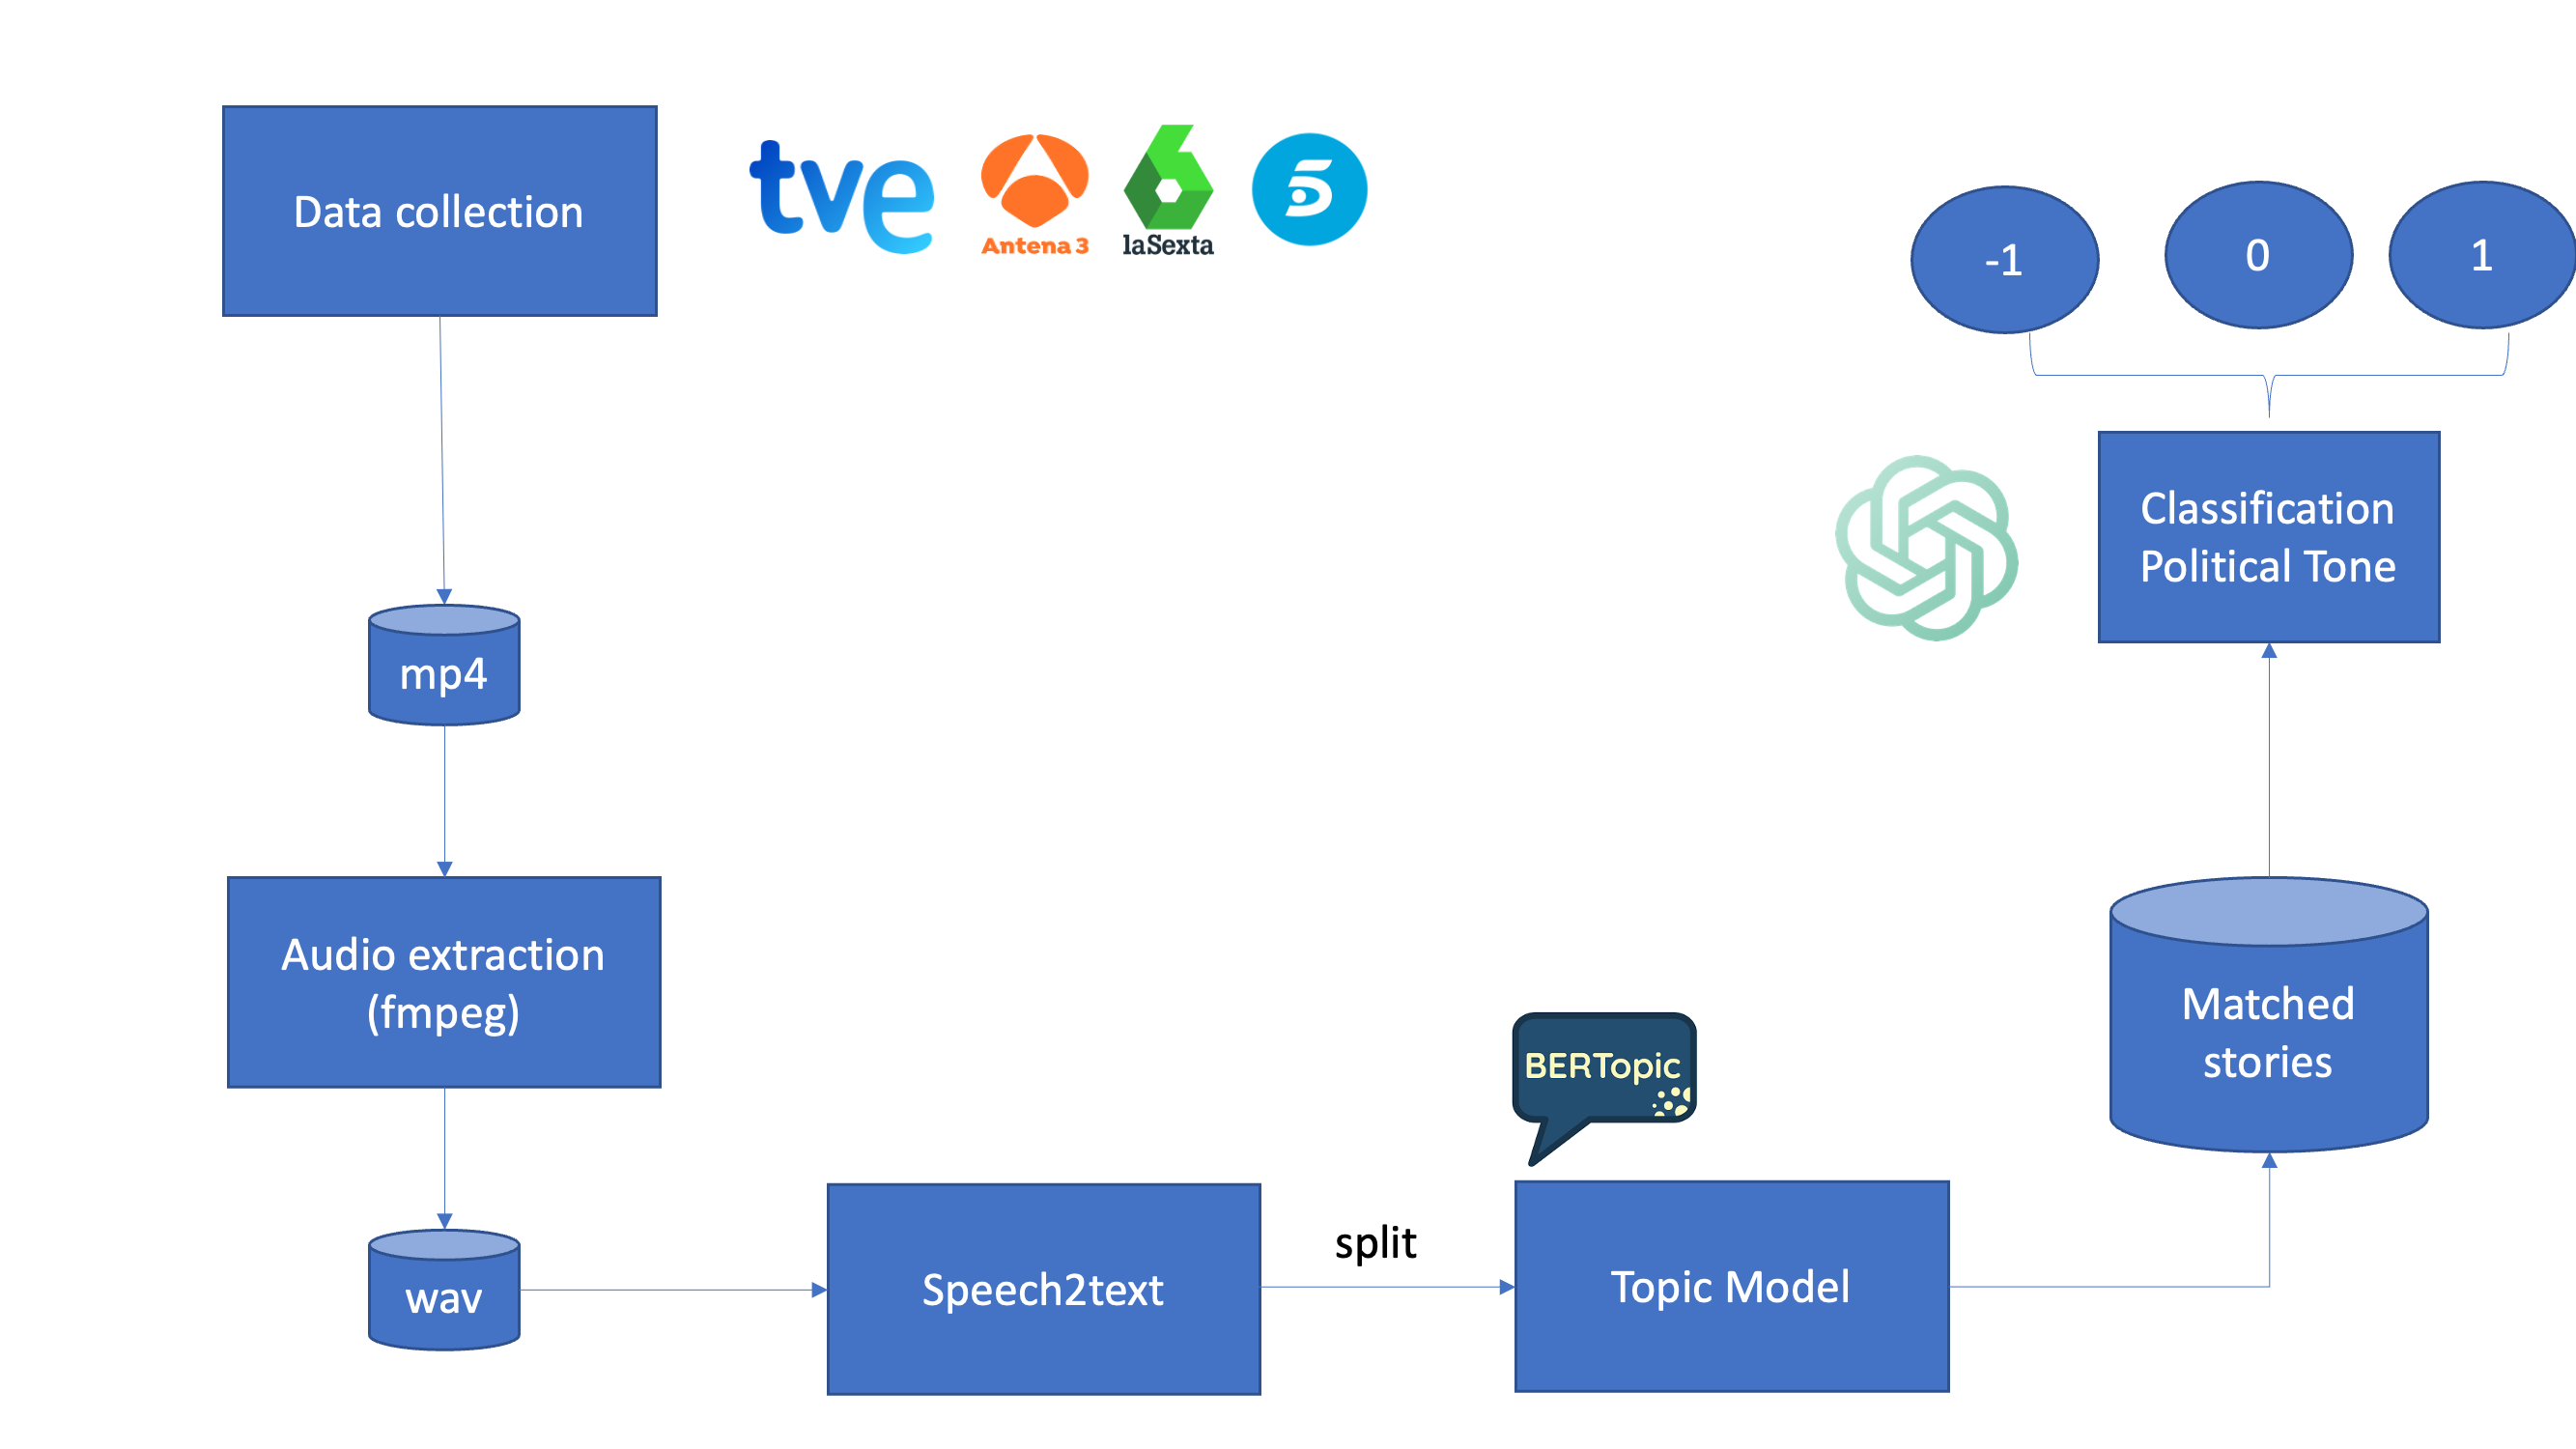
\includegraphics[width=150mm]{figures/pipeline3}
	\caption*{\small \textit{Note:} Pipeline for the text downloading. First videos are downloaded daily from the main TV channels. Google engine is used to convert the audio to text. I then split the stories by minute and use BERTopic to classify and match them. Finally, GPT4 is used to classify political tone.}
	\label{fig:pipeline}
\end{figure}



\textbf{Audio and transcription.} Each broadcast is converted from MP4 to mono PCM WAV to standardize the input for automatic speech recognition. Transcripts are obtained with \emph{Google Cloud Speech-to-Text} (language \texttt{es-ES}, long-running recognition with automatic punctuation). The service returns time-stamped transcripts; for each show I archive the raw JSON and a lightly normalized plaintext transcript.

\textbf{Segmentation and alignment.} Newscasts are split into minute-level stories using program timestamps and textual cues (anchor transitions and title cards). 

\textbf{Topic discovery.} Topics are estimated with \emph{BERTopic} using multilingual sentence embeddings (\texttt{paraphrase-multilingual-MiniLM-L12-v2}). After fitting, outlier reduction and topic updates are applied; residual or incoherent clusters are flagged and excluded from matched comparisons.

\textbf{LLM-based ideology classification.} Story-level political tone is obtained with ChatGPT on a discrete grid per party. To reduce computational and monetary costs, I first filter the set of minute-level stories using a dictionary of political keywords (Table~\ref{tab:politics}); the final classification set contains 15{,}406 stories. The prompt used in the classifier is:

\begin{tcolorbox}[colback=blue!5!white, colframe=blue!75!black, title=Prompt]
	Analyze the sentiment of the following news article with respect to the political parties (and their members) in Spain: PP, Podemos/Sumar, PSOE, VOX. Only use numeric values from the set [-1, -0.5, 0, 0.5, 1].
	
	Evaluate the sentiment towards each party with a number between -1 and 1, where -1 indicates an extremely negative perception, 0 indicates neutrality or irrelevance for the party, and 1 indicates an extremely positive perception.
	
	Consider only the values -1, -0.5, 0, 0.5, and 1.
	
	Base your evaluation solely on the explicit content of the news article. If the article does not mention or imply any sentiment towards a party, assign a 0 to that party.
	
	The format must always be a list \texttt{[PP
		, PSOE
		, UP
		, VOX
		]} where \texttt{X} represents the numeric sentiment value.
\end{tcolorbox}

\noindent\textit{Note:} Prompt used under \textit{gpt-4-0125-preview}. Story-level tones are aggregated to the program–day level with duration weights (seconds per story). Channel-level summaries are constructed by averaging across program–days, and matched-story comparisons are restricted to aligned topic–day pairs.



\newpage




\section{Robustness of the Text Classification}

\label{sec:robustness}







\subsection{Comparison with Previous Approaches}


One concern with LLMs classification is whether they can consistently capture meaningful patterns in text to distinguish tone. Table \ref{tab:top_trigrams} shows the most frequent three-word sequences across each sentiment–ideology category. The trigrams in the “Positive Right” column center on leadership titles and formal roles, reflecting an organizational focus; those in “Negative Right” cluster around legal and procedural language, indicating contexts of investigation or trial. The “Positive Left” trigrams emphasize policy areas and sectoral initiatives, suggesting substantive, topic-driven framing, while the “Negative Left” sequences feature judicial and procedural terms, pointing to oversight and legal scrutiny. Specific examples of stories can be seen in Appendix Table \ref{tab:examples_stories}.


To assess robustness, I also compare the LLM’s classifications with those obtained using methods from previous works \citep{gentzkow2010media,laver2003extracting}. I use all Spanish congress speeches during my sample period and exploit party labels to assess similarities with the outlets’ content. 


Similar to \cite{gentzkow2010media} and \cite{laver2003extracting} I exploit party ideology in congress speeches to calculate similarity measures of the outlet's speech. I make use of all congressional speeches produced during my sample period and associate each speaker with their respective political party, filtering to retain the set of relevant parties.

I follow a similar, non-linear version of \cite{laver2003extracting} and create a score for each word $w$ in the congress speech as: 



\begin{equation}
	\text{Score}(w) \;=\; \ln \left( \frac{\mathrm{freq}(w,\text{Left}) + \alpha}{\mathrm{Total}_{\text{Left}} + \alpha} \right) \;-\; \ln \left( \frac{\mathrm{freq}(w,\text{Right}) + \alpha}{\mathrm{Total}_{\text{Right}} + \alpha} \right),
	\label{eq:log_ratio}
\end{equation}

where:
\begin{itemize}
	\item $\mathrm{freq}(w,\text{Left})$ is the number of times word $w$ appears in the speeches of left-leaning parties (PSOE and UP),
	\item $\mathrm{Total}_{\text{Left}}$ is the total word count in left-party speeches,
	\item $\mathrm{freq}(w,\text{Right})$ and $\mathrm{Total}_{\text{Right}}$ are defined analogously for right-leaning parties (PP and Vox), and
	\item $\alpha$ is a small smoothing parameter.
	
\end{itemize}

I select the value of alpha that maximizes accuracy of label prediction in the congress dataset; $\alpha=0.9$.	
Words with high positive scores are used disproportionately in left-leaning speeches, while those with high negative scores are more characteristic of right-leaning speeches. I rank all words by their computed score and select the top 100 left-coded words and top 100 right-coded words, represented in  Figure  \ref{fig:wordcloud}. 






\begin{figure}[htbp!]
	\caption{Word Cloud Congress Speeches}
	
	\centering
	%— Left pane —
	\begin{minipage}{0.46\textwidth}
		\centering
		\textbf{(a) Top Left Words}\\[1ex]
		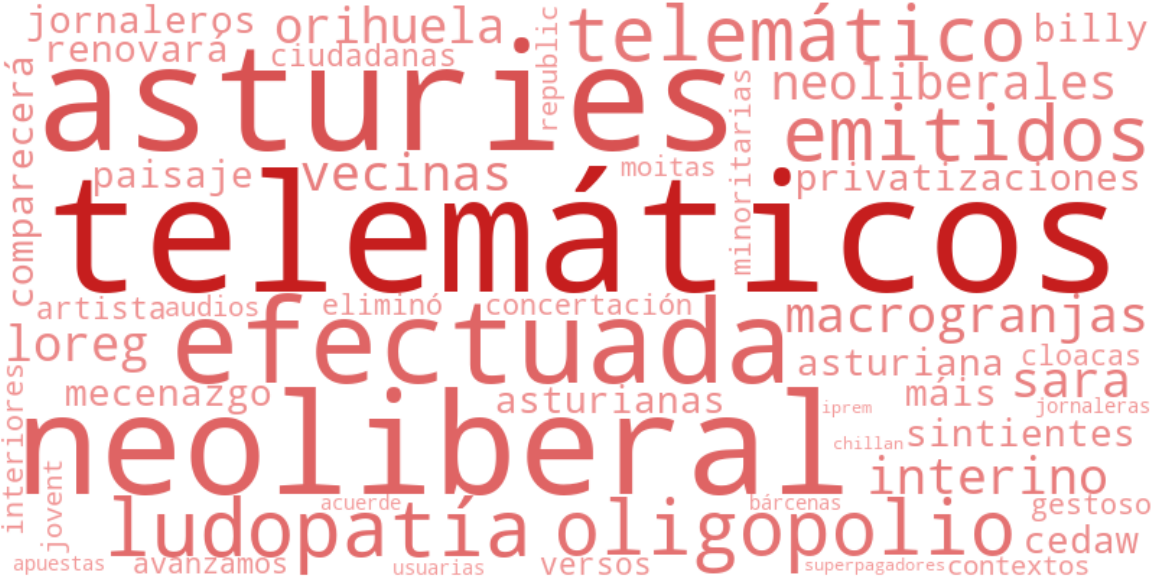
\includegraphics[width=\linewidth]{figures/congress_left.pdf}
	\end{minipage}%
	\hfill
	%— Right pane —
	\begin{minipage}{0.46\textwidth}
		\centering
		\textbf{(b) Top Right Words}\\[1ex]
		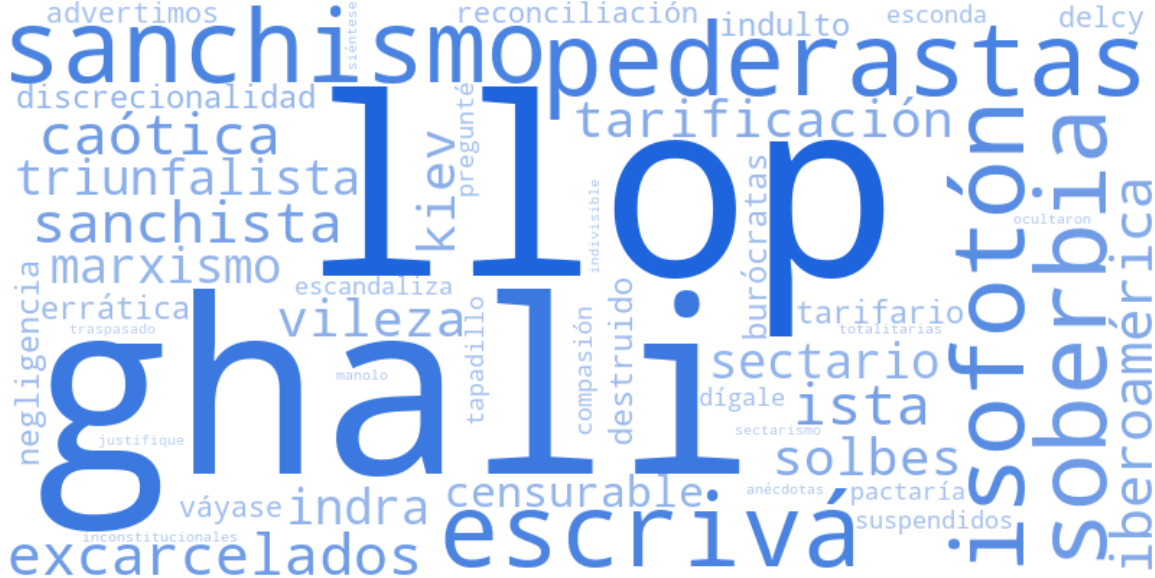
\includegraphics[width=\linewidth]{figures/congress_right.pdf}
	\end{minipage}
	
	%— Shared caption and note —
	
	
	\vspace{0.5ex}
	

		\caption*{\small \textit{Note:} The wordclouds represent the top words with lowest (left) and highest (right) scores as defined in Eq.~\eqref{eq:log_ratio}. Size is weighted by word TF-IDF value.}
	
	\label{fig:wordcloud}	
\end{figure}



The word clouds make clear the distinctive use of language by parties in congress. On the left, for example, the large term “neoliberal” (neoliberalism) underscores an ongoing critique of market‐driven reforms, while “oligopolio” (oligopoly) highlights concerns about concentrated economic power. On the right, “sanchismo” (literally “Sánchez-ism”) signals frequent reference to the governing style of Prime Minister Sánchez as a political brand, and “pederastas” (pederasts) reveals the use of morally charged scandal language with the ley solo sí es si scandal. 





Figure \ref{fig:congress_line} shows the left–right positions derived from this method. Although the overall ranking of the outlets from left to right is consistent with the ChatGPT classification in Figure \ref{fig:chat}, the middle channel is now classified as left-wing, close to the public channel. 


\begin{comment}
	content...

\begin{figure}[htbp!]
	\centering
	\caption{Normalized Ideology Scores from Congress Speeches}
	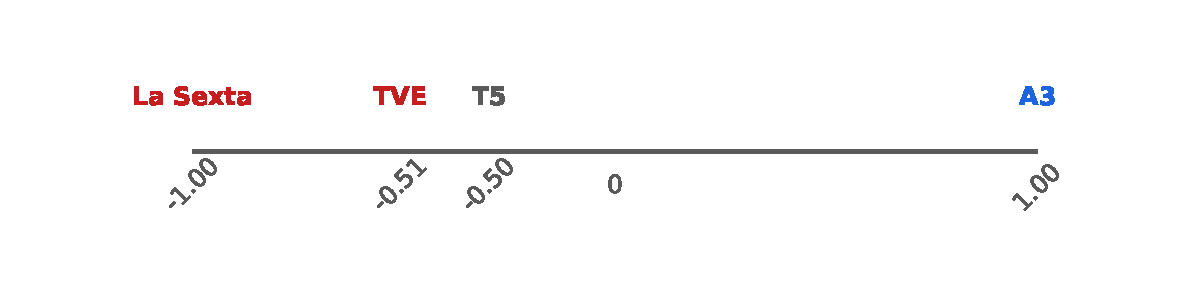
\includegraphics[width=120mm]{figures/congress_line}
	\caption*{\small  \textit{Note:} The figure shows the normalized ideology positions of the channels after the text classification based on congress speeches as described by Equation \ref{eq:log_ratio}}

\end{figure}
\end{comment}






	\begin{figure}[!htbp]
	\centering
	\caption{Normalized Ideology Index by Channel}
	
	% Panel (a): ChatGPT-based
	\begin{minipage}[t]{0.49\textwidth}
		\centering
		(a) Demand: Viewers' ideology
		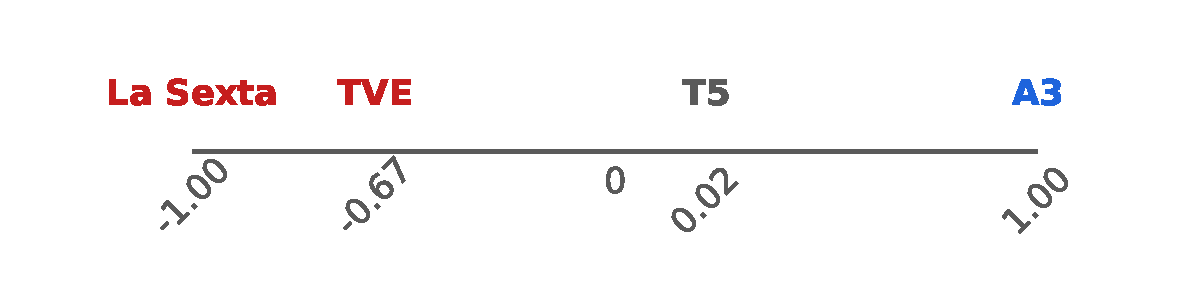
\includegraphics[width=\linewidth]{figures/congress_line_cis}
	\end{minipage}
	\hfill
	% Panel (b): CIS-based
	\begin{minipage}[t]{0.49\textwidth}
		\centering
		
		
		(b) Supply: Text classification 
		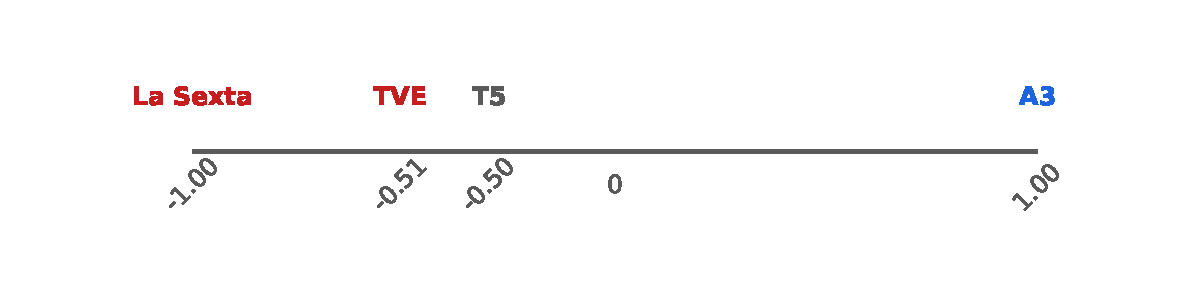
\includegraphics[width=\linewidth]{figures/congress_line}
		

	\end{minipage}
	
	
	\caption*{\small \textit{Note:} The figure compares normalized left–right positions for the outlets in the sample. Panel (a) uses viewer ideology data from CIS survey data, using the difference in correlation coefficients between right and left; panel (b) uses ChatGPT-based text classification net tone as described in Equation \eqref{eq:log_ratio}. Values are normalized so that the two most extreme channels take values -1 and 1. }
	\label{fig:congress_line}
\end{figure}




Two remarks are worth mentioning. First, it is important to note that this comparison against survey data might entail some issues. Declared preferences can serve as validation under the assumption of channels' decisions being heavily driven by demand preferences rather than other factors. Cross-validation of human annotators on the labels of political stories would be an alternative way to verify the results. 

Second, reducing each story to a single left–right score aids interpretation, but ignores the multidimensional nature of politics highlighted by \citet{puglisi2011newspapers}. Economic versus cultural cleavages, or regional versus national frames, may evolve differently and deserve separate tracking. I leave extending the LLM classifier to a low-dimensional vector of ideological dimensions for future work.




\subsection{Stability of the Classifier}


Due to their inherent stochasticity, repeated queries using the same prompt may yield different classifications \citep{llmstability2024}. As shown in \citep{llmclassification2024}, this variability can introduce noise in tasks that require high consistency, particularly in content classification. To mitigate this issue, I leverage OpenAI’s “functions” tool, which constrains the classifier’s responses to predefined discrete numerical outputs, reducing potential inconsistencies. Table \ref{tab:table_stability} presents the mean classification scores from 100 iterations of a random sample of political stories \footnote{Good practices recommend to run the classification multiple times and average out the results \citep{tornberg2023}. Financial costs, however, impede me from doing the whole approach multiple times}, along with the corresponding standard errors. The relatively small standard errors suggest that, despite the model’s stochastic nature, the classification remains stable.





\begin{table}[!htb]
	\centering
	\caption{Mean and Standard Error for 100 Rounds of ChatGPT Classification}
	\begin{tabular}{|l|c|c|c|c|}
		\hline
		\textbf{Statistic} & \textbf{PP} & \textbf{PSOE} & \textbf{VOX} & \textbf{UP} \\
		\hline
		Mean & -0.014 & 0.106 & -0.053 & 0.024 \\
		Standard Error & 0.003 & 0.004 & 0.001 & 0.002 \\
		\hline
	\end{tabular}
	\caption*{\small \textit{Note:}  The table shows the mean and standard error for 100 rounds of ChatGPT classification of political content with 40 random political stories.}
	\label{tab:table_stability}
\end{table}









\subsection{Text vs.\ Image}




Imagery is a key component of television. This may be especially relevant for political actors, for whom televised coverage has been shown to magnify the impact of candidates’ physical appearance on voter perceptions and electoral outcomes \citep{Lenz2011LookingTP}. Imagery in the form of time devoted to candidates further constitutes the main metric used by regulatory agencies. For example, the French media authority ARCOM publishes monthly “pluralism” reports that track each political actor’s share of speaking time on national television; Italy’s Osservatorio di Pavia produces similar statistics for the national regulator AGCOM. These metrics have also been used extensively in research as measures of slant \citep[see, e.g.,][]{CageHengelHerveUrvoy2022,durante2012partisan}.

Here I compare some of these approaches to my text-based measure. Due to computational constraints, I cannot perform image detection across my full video sample. Instead, I compare image-based and text-based metrics using a random sample of 67 days. Specifically, I train a state-of-the-art face recognition system \citep{face_recognition} using labeled images of the main party leaders: Pedro Sánchez (PSOE), Alberto Núñez Feijóo (PP), Santiago Abascal (VOX), and Yolanda Díaz (UP). I then extract frames from the first 25 minutes of each prime time news broadcast across major channels, resulting in a sample of 79,788 images. Using the \texttt{face\_recognition} library, I detect and identify faces in each frame. This allows me to construct a frame-level dataset of visual exposure, which I aggregate at the daily level for each channel and party leader.

The net tone on the sample of days for each channel and political leader is shown in Figure 	\ref{fig:tone_channel}. As expected, significant differences appear, positioning channels in the left-right spectrum shown before. 


\begin{figure}[htbp!]
	\caption{Net Tone per Channel and Politician}
	\centering
	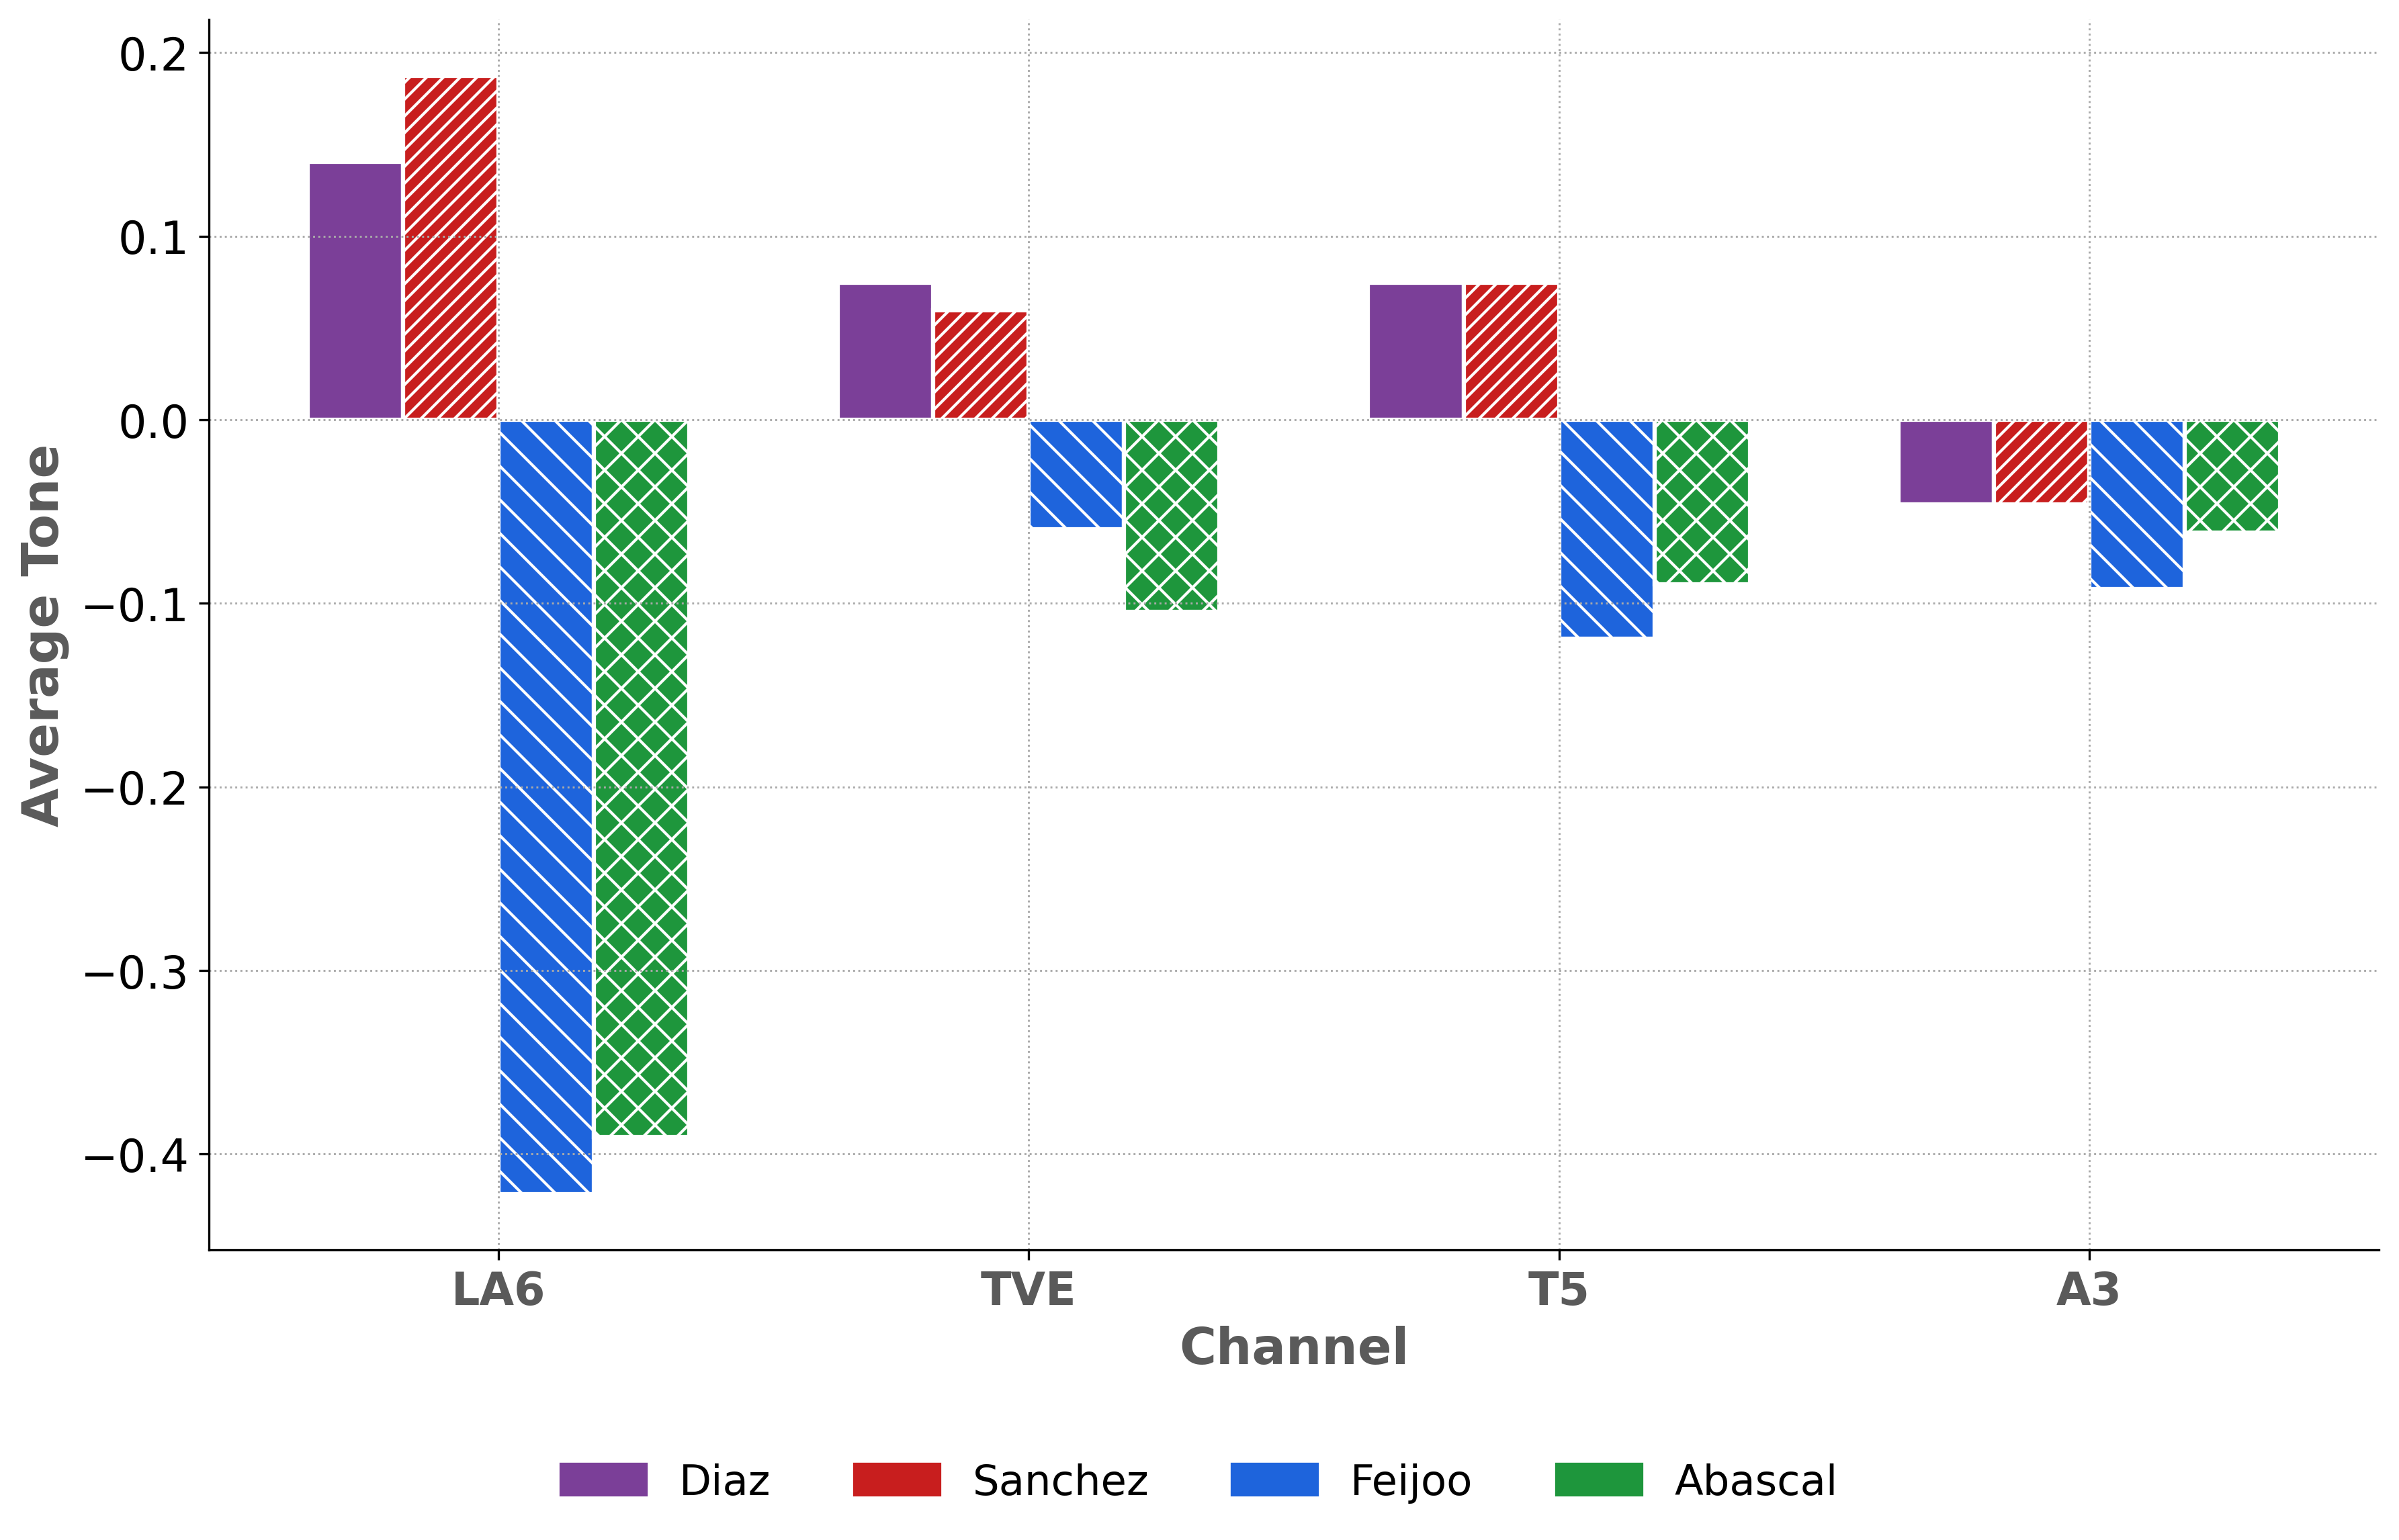
\includegraphics[width=150mm]{figures/politicians_tone_proportions}
	\caption*{\small \textit{Note:} The figure shows the net tone based on the ChatGPT classification by political actor and channel for a random sample of 67 days. }
	\label{fig:tone_channel}
\end{figure}





Next, I compare if visuals or tone follow a similar scenario. Figure \ref{fig:combined_channel} panel a) shows the proportion of image appearances by channel and political leader. All channels coincide in their ranking, giving more air to PP, followed by PSOE, UP, and VOX. The two most extreme channels—La Sexta on the left and A3 on the right—give very similar coverage to the right-wing politician Feijóo, appearing in nearly 2\% of the frames. Panel b)  reveals a similar pattern for text mentions of the party leaders.


\begin{figure}[htbp!]
	\centering
	\caption{Proportion of appearances by political actor and channel. Panel (a) shows image appearances and panel (b) shows text mentions for a random sample of 67 days.}
	
	%— Left panel —
	\begin{minipage}{0.48\textwidth}
		\centering
		\textbf{(a) Image appearances}\\[1ex]
		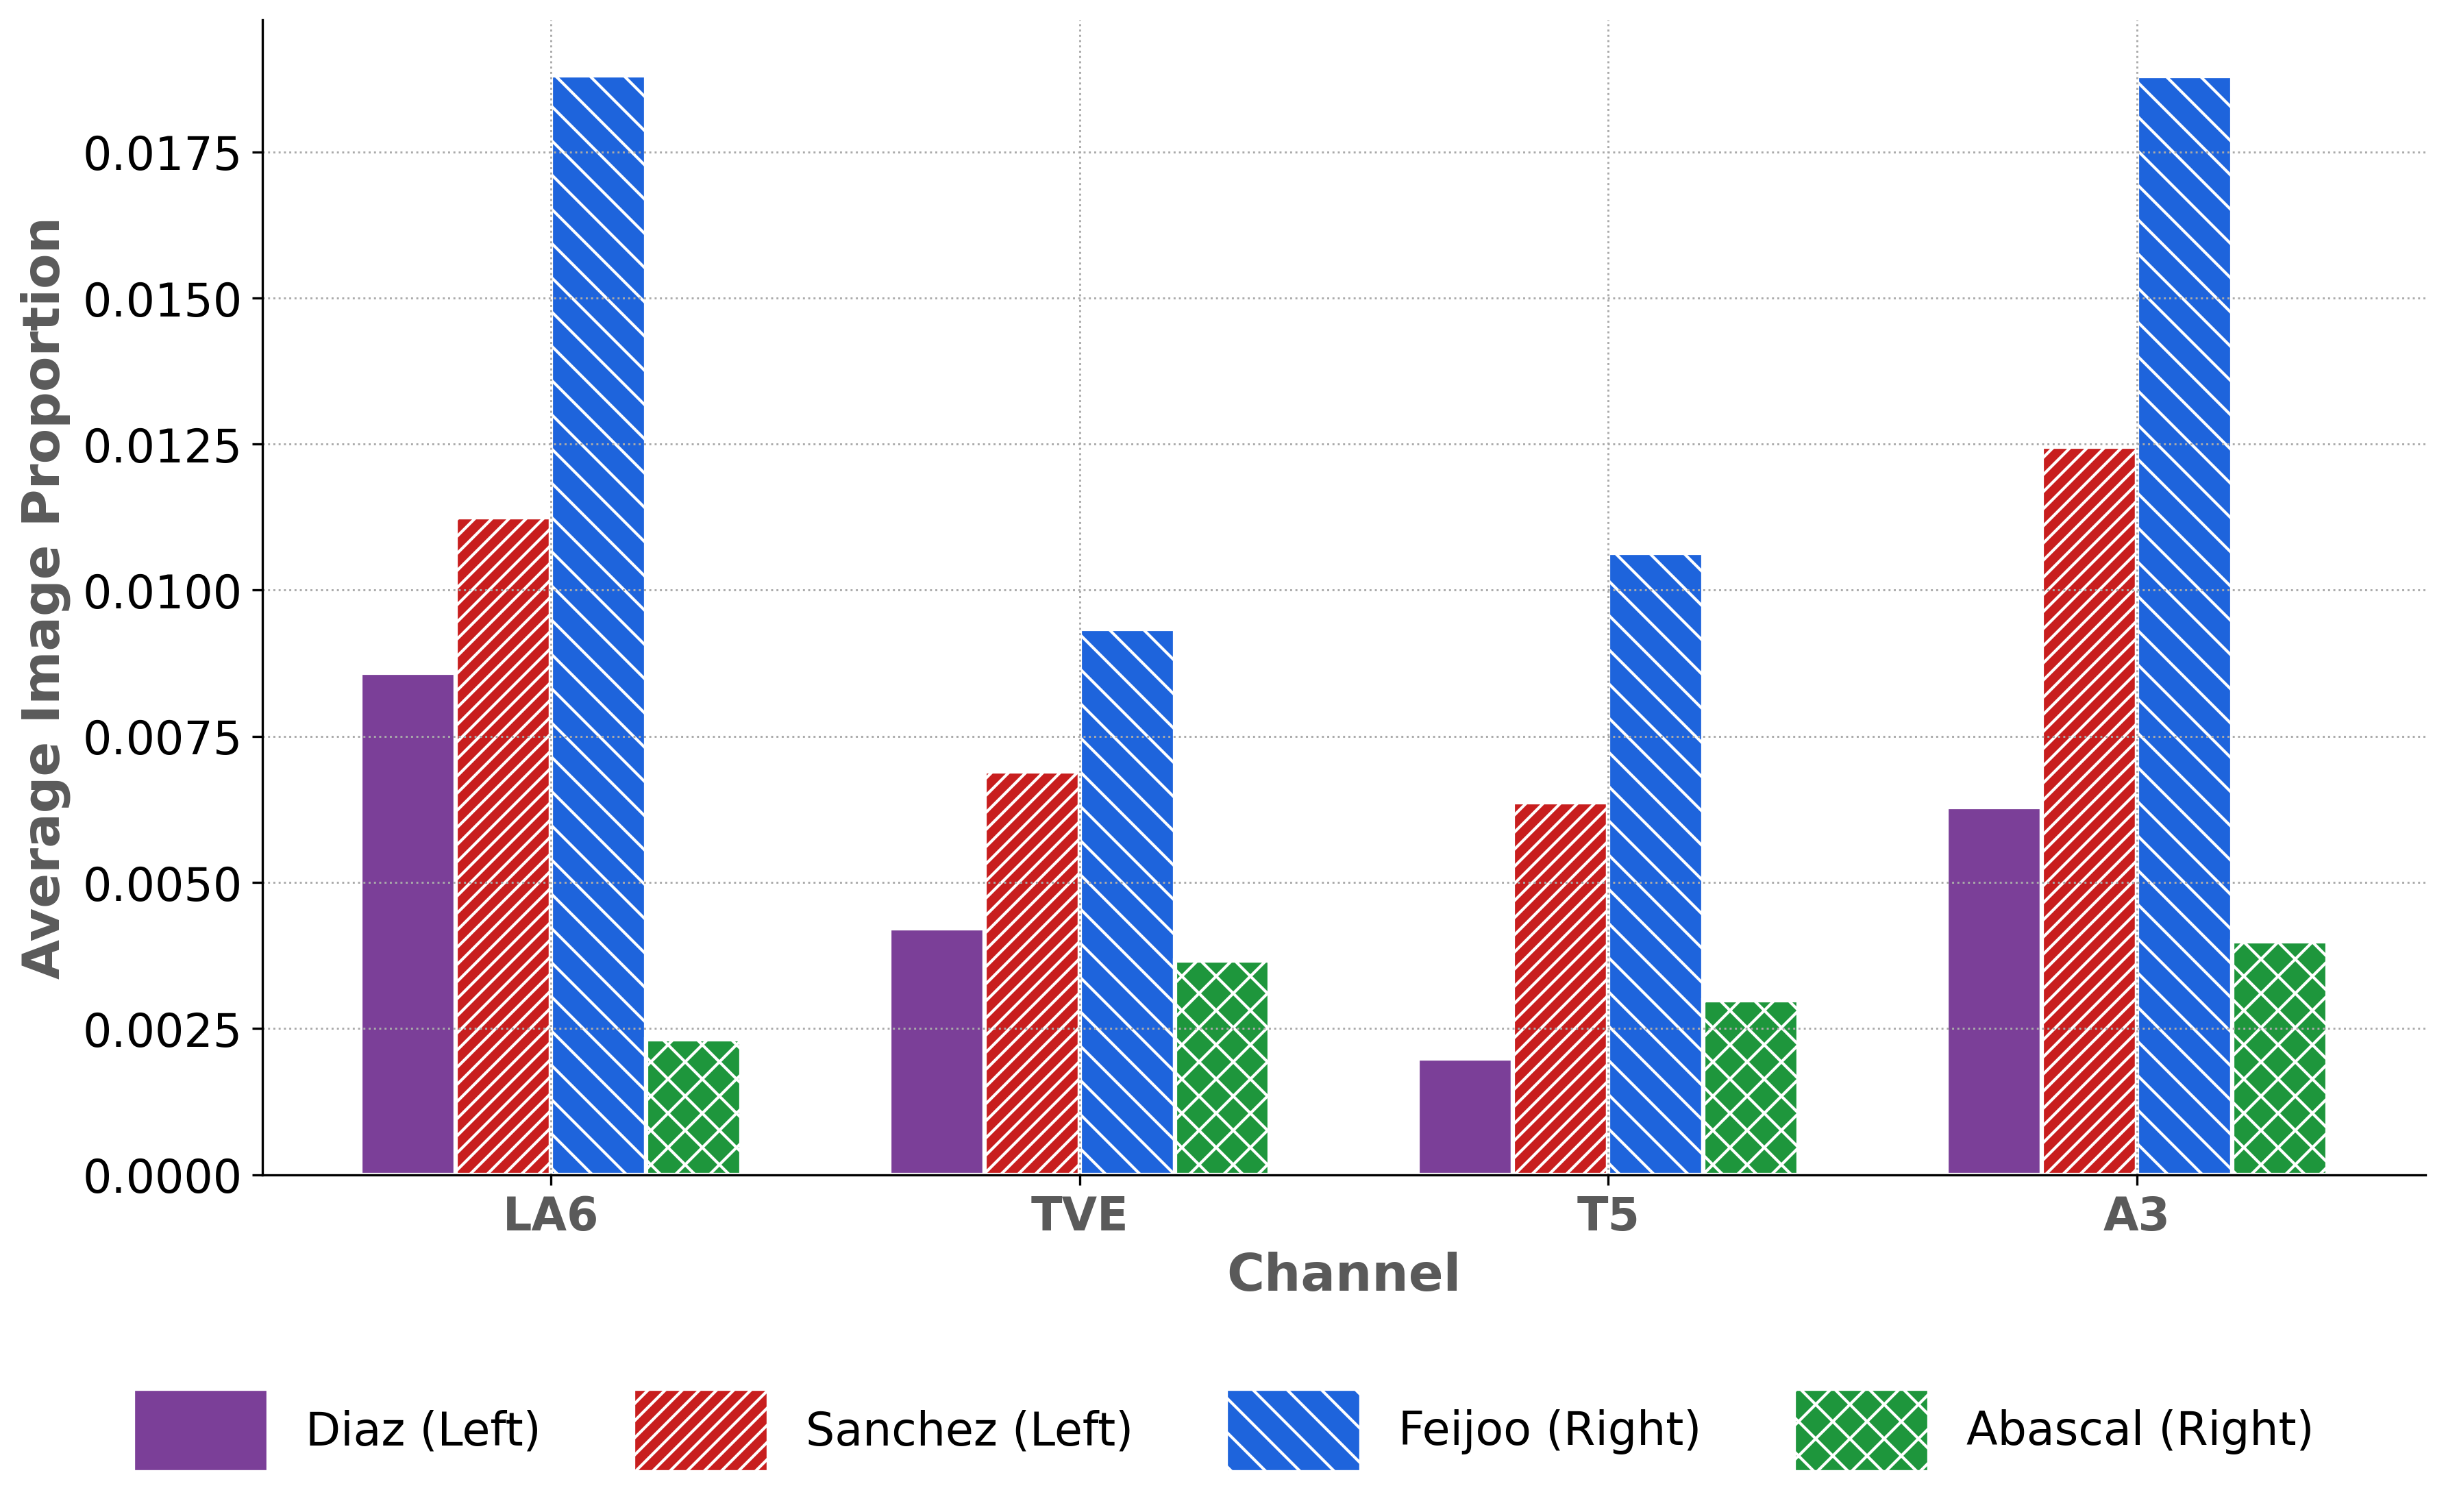
\includegraphics[width=\linewidth]{figures/politicians_image_proportions}
	\end{minipage}%
	\hfill
	%— Right panel —
	\begin{minipage}{0.48\textwidth}
		\centering
		\textbf{(b) Text mentions}\\[1ex]
		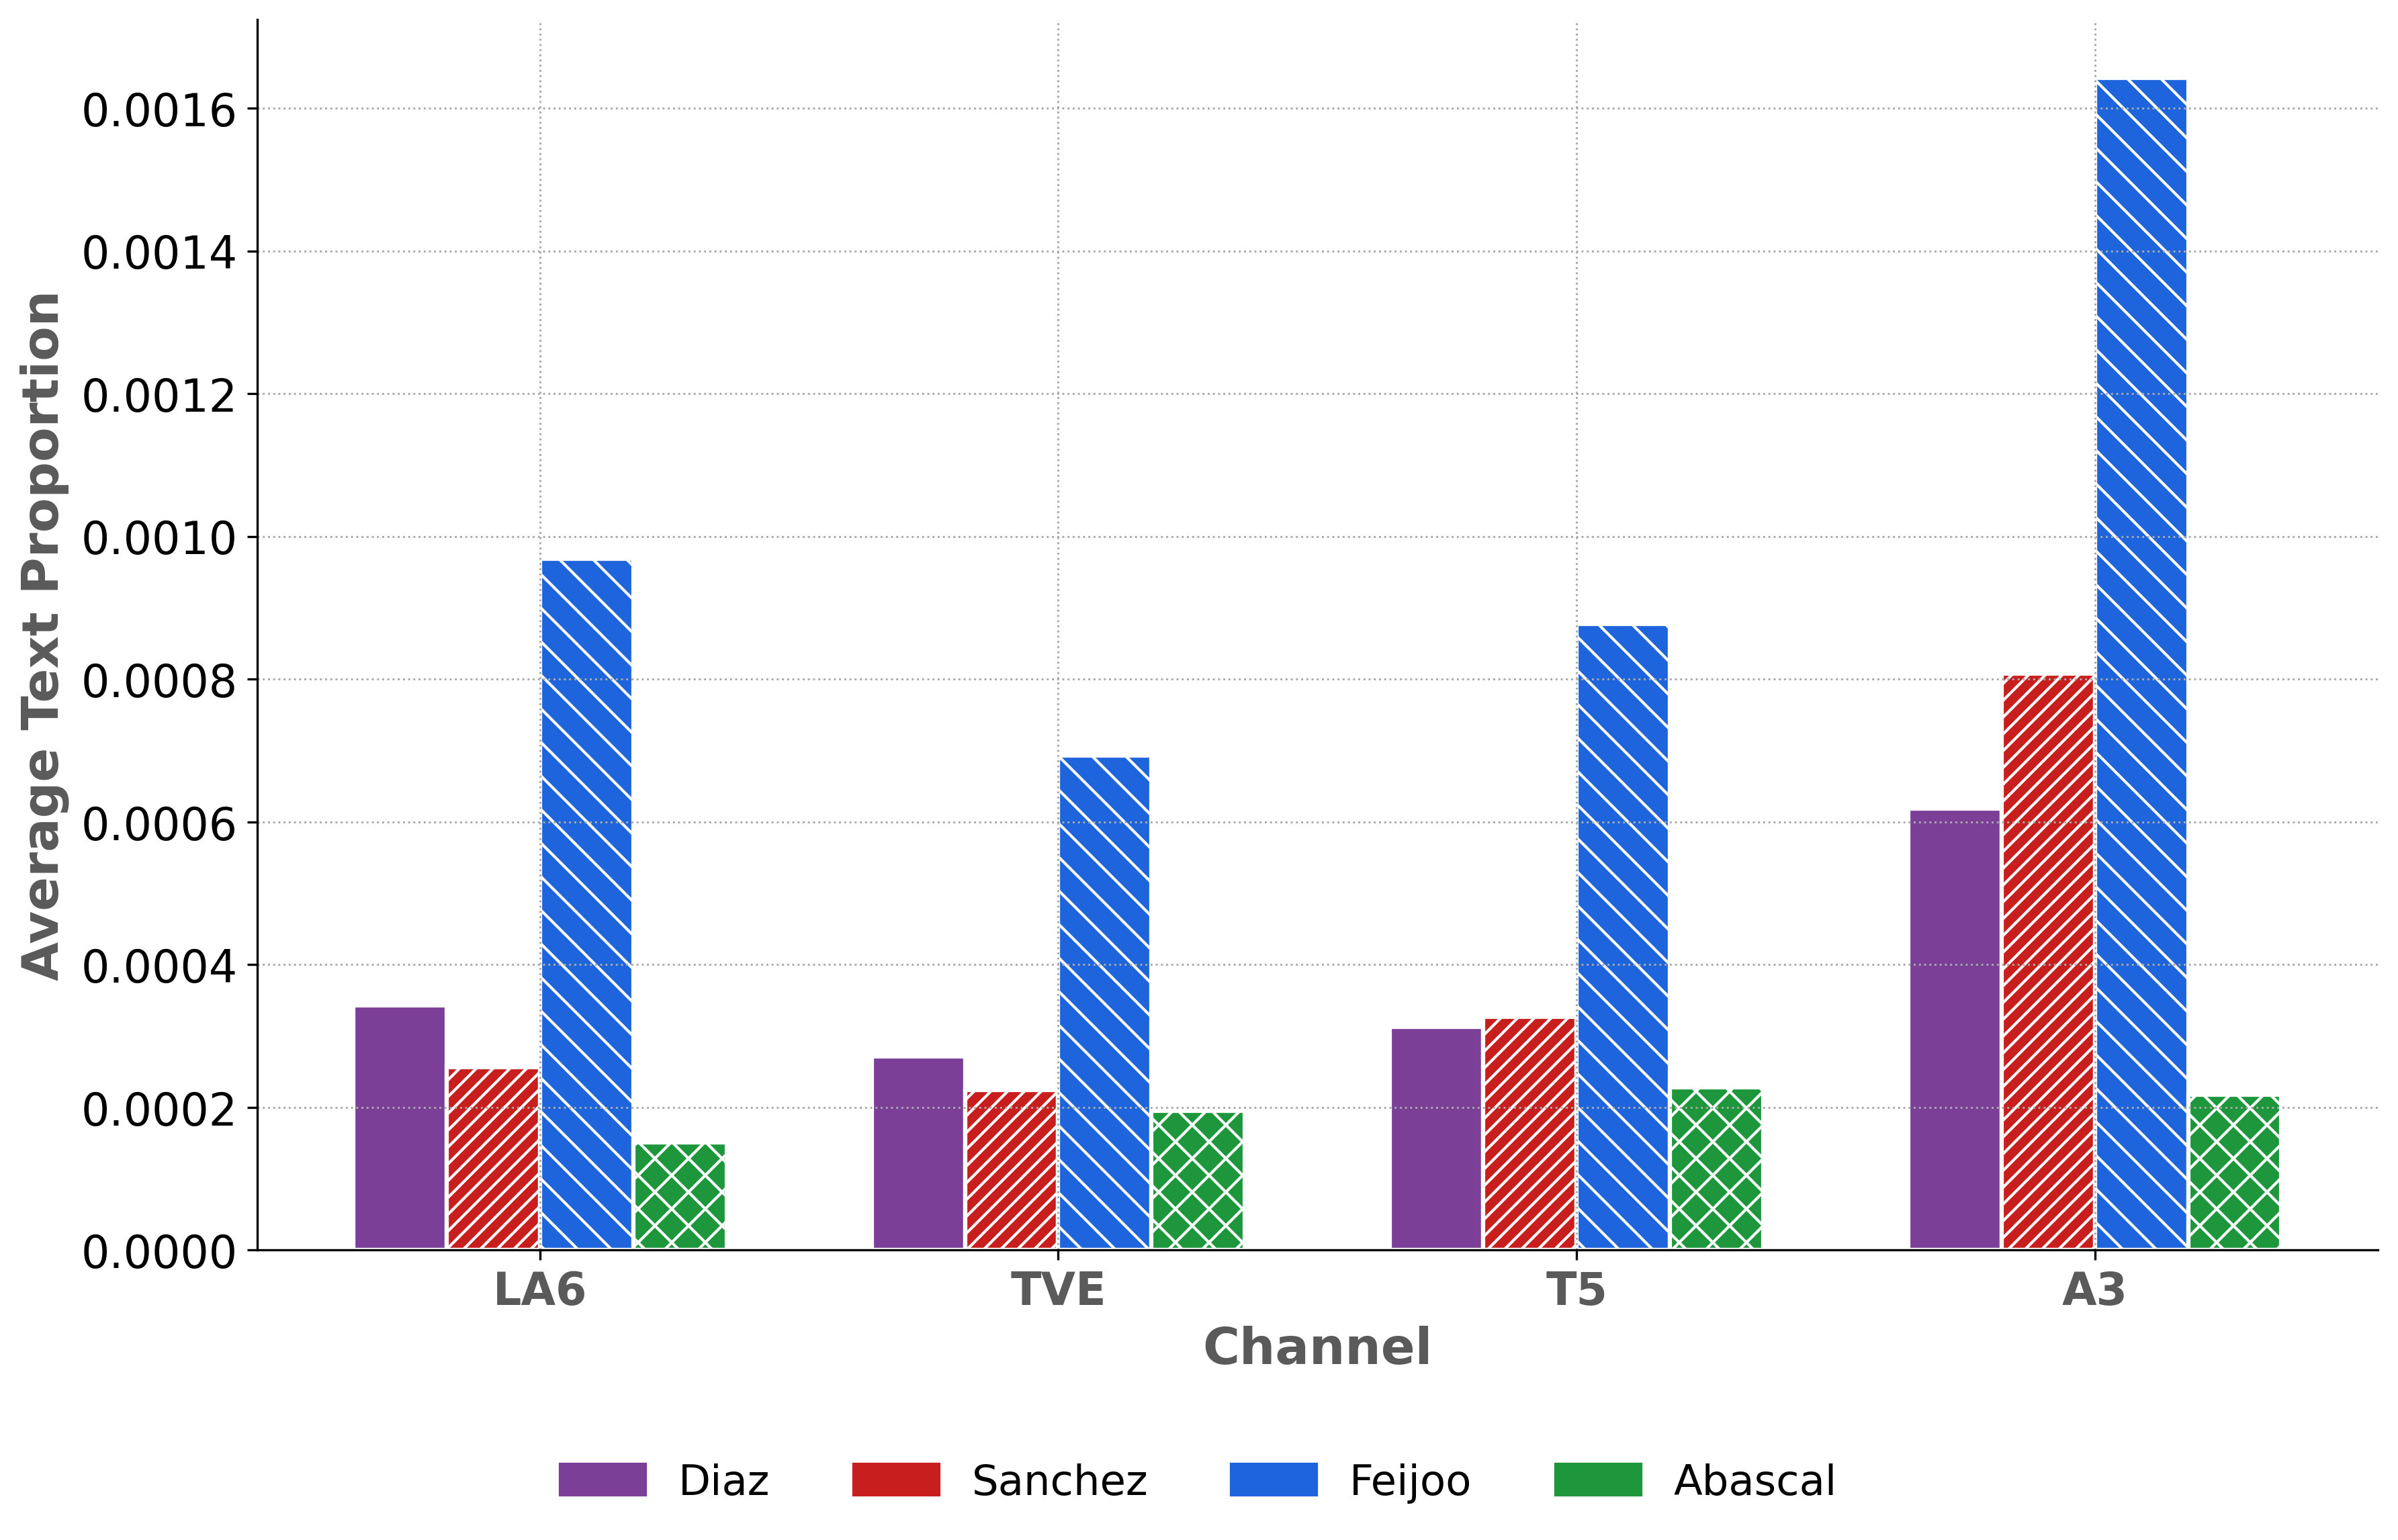
\includegraphics[width=\linewidth]{figures/politicians_text_proportions}
	\end{minipage}
	
	\vspace{1ex}
	
\caption*{\small
		\textit{Note:} The proportions are computed per channel and political actor over the same random sample of 67 days.}
	\label{fig:combined_channel}
\end{figure}



To further examine the relationship between tone—based on the LLM classification—and coverage, I regress net tone by political actor on both the proportion of image appearances and word mentions. Table \ref{tab:images2} reports results under different specifications, including date and channel fixed effects.




\begin{table}[htbp!]
	\centering
	
	\caption{Effect of Mentions on Tone toward Party Leaders}
	\label{tab:images2}
	\small
	\setlength{\tabcolsep}{4pt}
	\renewcommand{\arraystretch}{1.0}
	\begin{tabular}{lcccc}
		\toprule
		& \multicolumn{4}{c}{\textit{Outlet Slant} (\(x\))} \\
		\cmidrule(lr){2-5}
		& (1) & (2) & (3) & (4) \\
		\midrule
		
		\multicolumn{5}{l}{\textbf{Feijóo (PP)}}\\
		Text Mentions     &  -1.956         &  -3.038         &   0.364         &   -1.342        \\
		&  (2.063)        &  (2.134)        &  (2.391)        &  (2.584)        \\
		Image Appearances &  -0.065         &   0.003         &  -0.275         &  -0.189         \\
		&  (0.147)        &  (0.151)        &  (0.179)        &  (0.189)        \\
		\addlinespace
		\hline
		\multicolumn{5}{l}{\textbf{Abascal (VOX)}}\\
		Text Mentions     & -42.813& -44.024& -46.659& -49.989\\
		&  (7.855)        &  (7.832)        &  (9.609)        &  (9.471)        \\
		Image Appearances &   0.963 &   0.933&   0.565         &   0.437         \\
		&  (0.470)        &  (0.470)        &  (0.600)        &  (0.595)        \\
		\addlinespace
		\hline
		\multicolumn{5}{l}{\textbf{Sánchez (PSOE)}}\\
		Text Mentions     &   4.131         &  11.634 &   2.648         &  13.515  \\
		&  (6.020)        &  (6.992)        &  (6.494)        &  (7.909)        \\
		Image Appearances &   0.023         &  -0.045         &   0.033         &   0.032         \\
		&  (0.239)        &  (0.244)        &  (0.356)        &  (0.377)        \\
		\addlinespace
		\hline
		\multicolumn{5}{l}{\textbf{Díaz (UP)}}\\
		Text Mentions     &  -0.576         &   1.276         &  -0.714         &   3.365         \\
		&  (3.158)        &  (3.280)        &  (4.080)        &  (4.405)        \\
		Image Appearances &   0.473&   0.485 &   0.290         &   0.321         \\
		&  (0.197)        &  (0.206)        &  (0.232)        &  (0.247)        \\
		\midrule
		Channel FE        & No              & Yes             & No              & Yes             \\
		Date FE           & No              & No              & Yes             & Yes             \\
		\midrule
		Observations      & 231             & 231             & 231             & 227             \\
		\bottomrule
	\end{tabular}
	
	\vspace{0.5em}
	\begin{flushleft}
		\small \textit{Note:} Robust standard errors in parentheses.
		%\sym{*} \(p<0.05\), \sym{**} \(p<0.01\), \sym{***} \(p<0.001\).  
		Each block shows coefficients from regressing net tone on text mentions and image appearances of the party leader.
	\end{flushleft}
\end{table}



Column~(4) reports the specification with both channel and day of the week fixed effects, so the coefficients reflect pure within–channel–day fluctuations in coverage. The pattern is heterogeneous across politicians. For Abascal (VOX), a one-standard-deviation increase in word mentions predicts a decrease of $0.39$ standard deviations in tone, whereas the same increase in on-screen images predicts an increase of $0.06$ standard deviations. Both left-leaning politicians present positive correlations between image appearances and tone, although neither appears to be a strong predictor.

Taken together, the results indicate that text-based and image-based measures of salience relate to tone in systematically different ways. Outlets appear much more homogeneous under this metric, with extreme channels showing similar values. This poses concerns regarding the interpretation of previous metrics based on airtime.




%\clearpage


\section{Figures}
	
	
	
	\begin{figure}[!htbp]
		\centering
		\caption{Top Media Source to Acquire Political Information in Spain}
		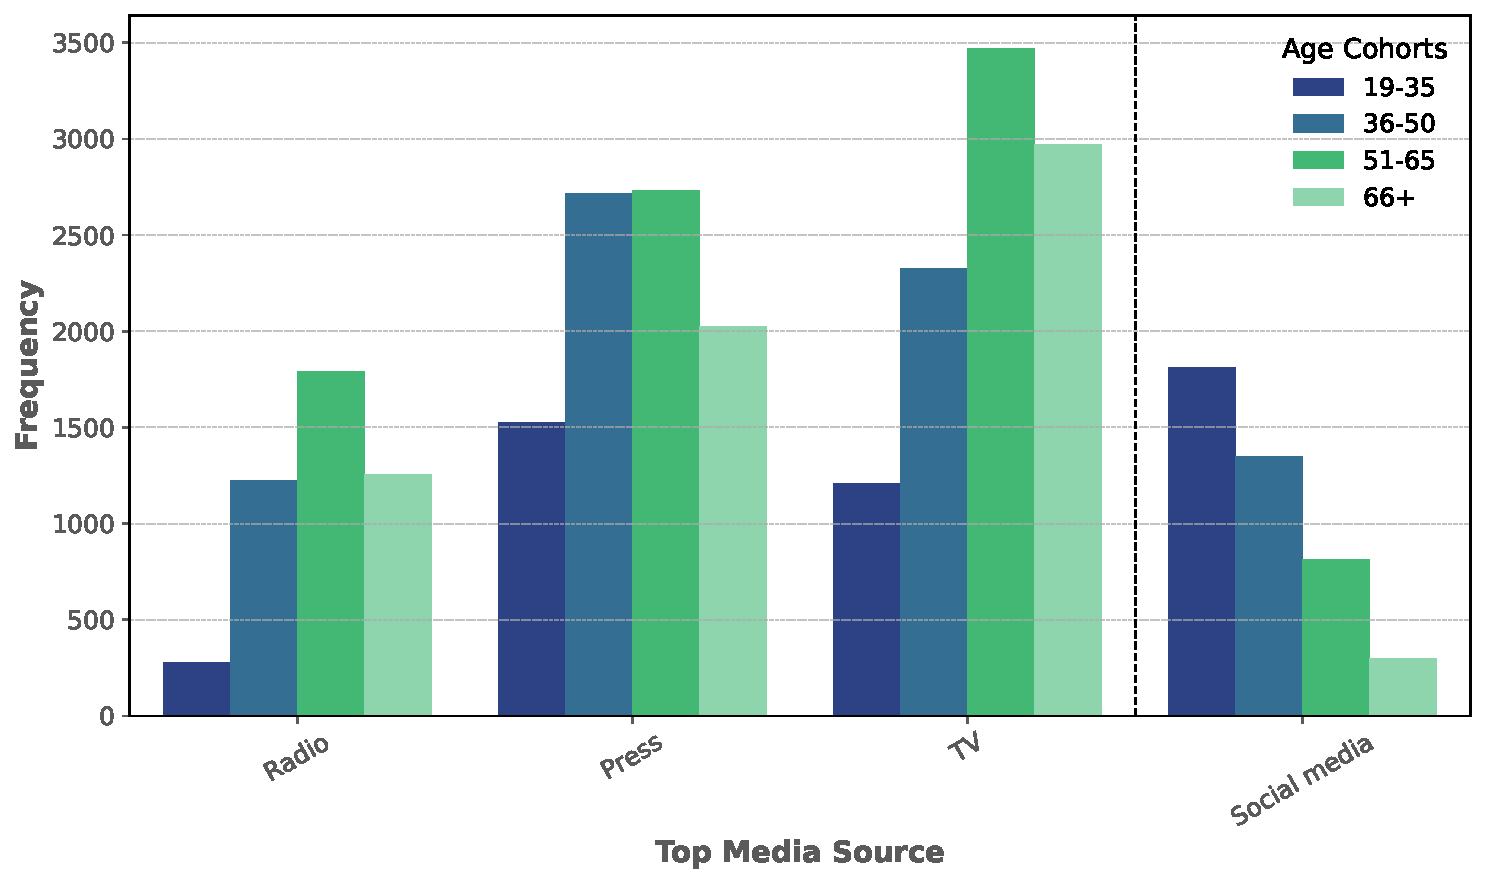
\includegraphics[width=130mm]{figures/age_cohorts}
		\caption*{\small \textit{Note:} Histogram on the preferred media used for political information by age cohorts in Spain.  
			Source: Barómetro CIS, 2023. }
		\label{fig:motivation}
	\end{figure}
	

	
	
	
	\begin{figure}[!htb]
		\caption{Tone across Channels and Parties off and during Campaign }
		\centering
		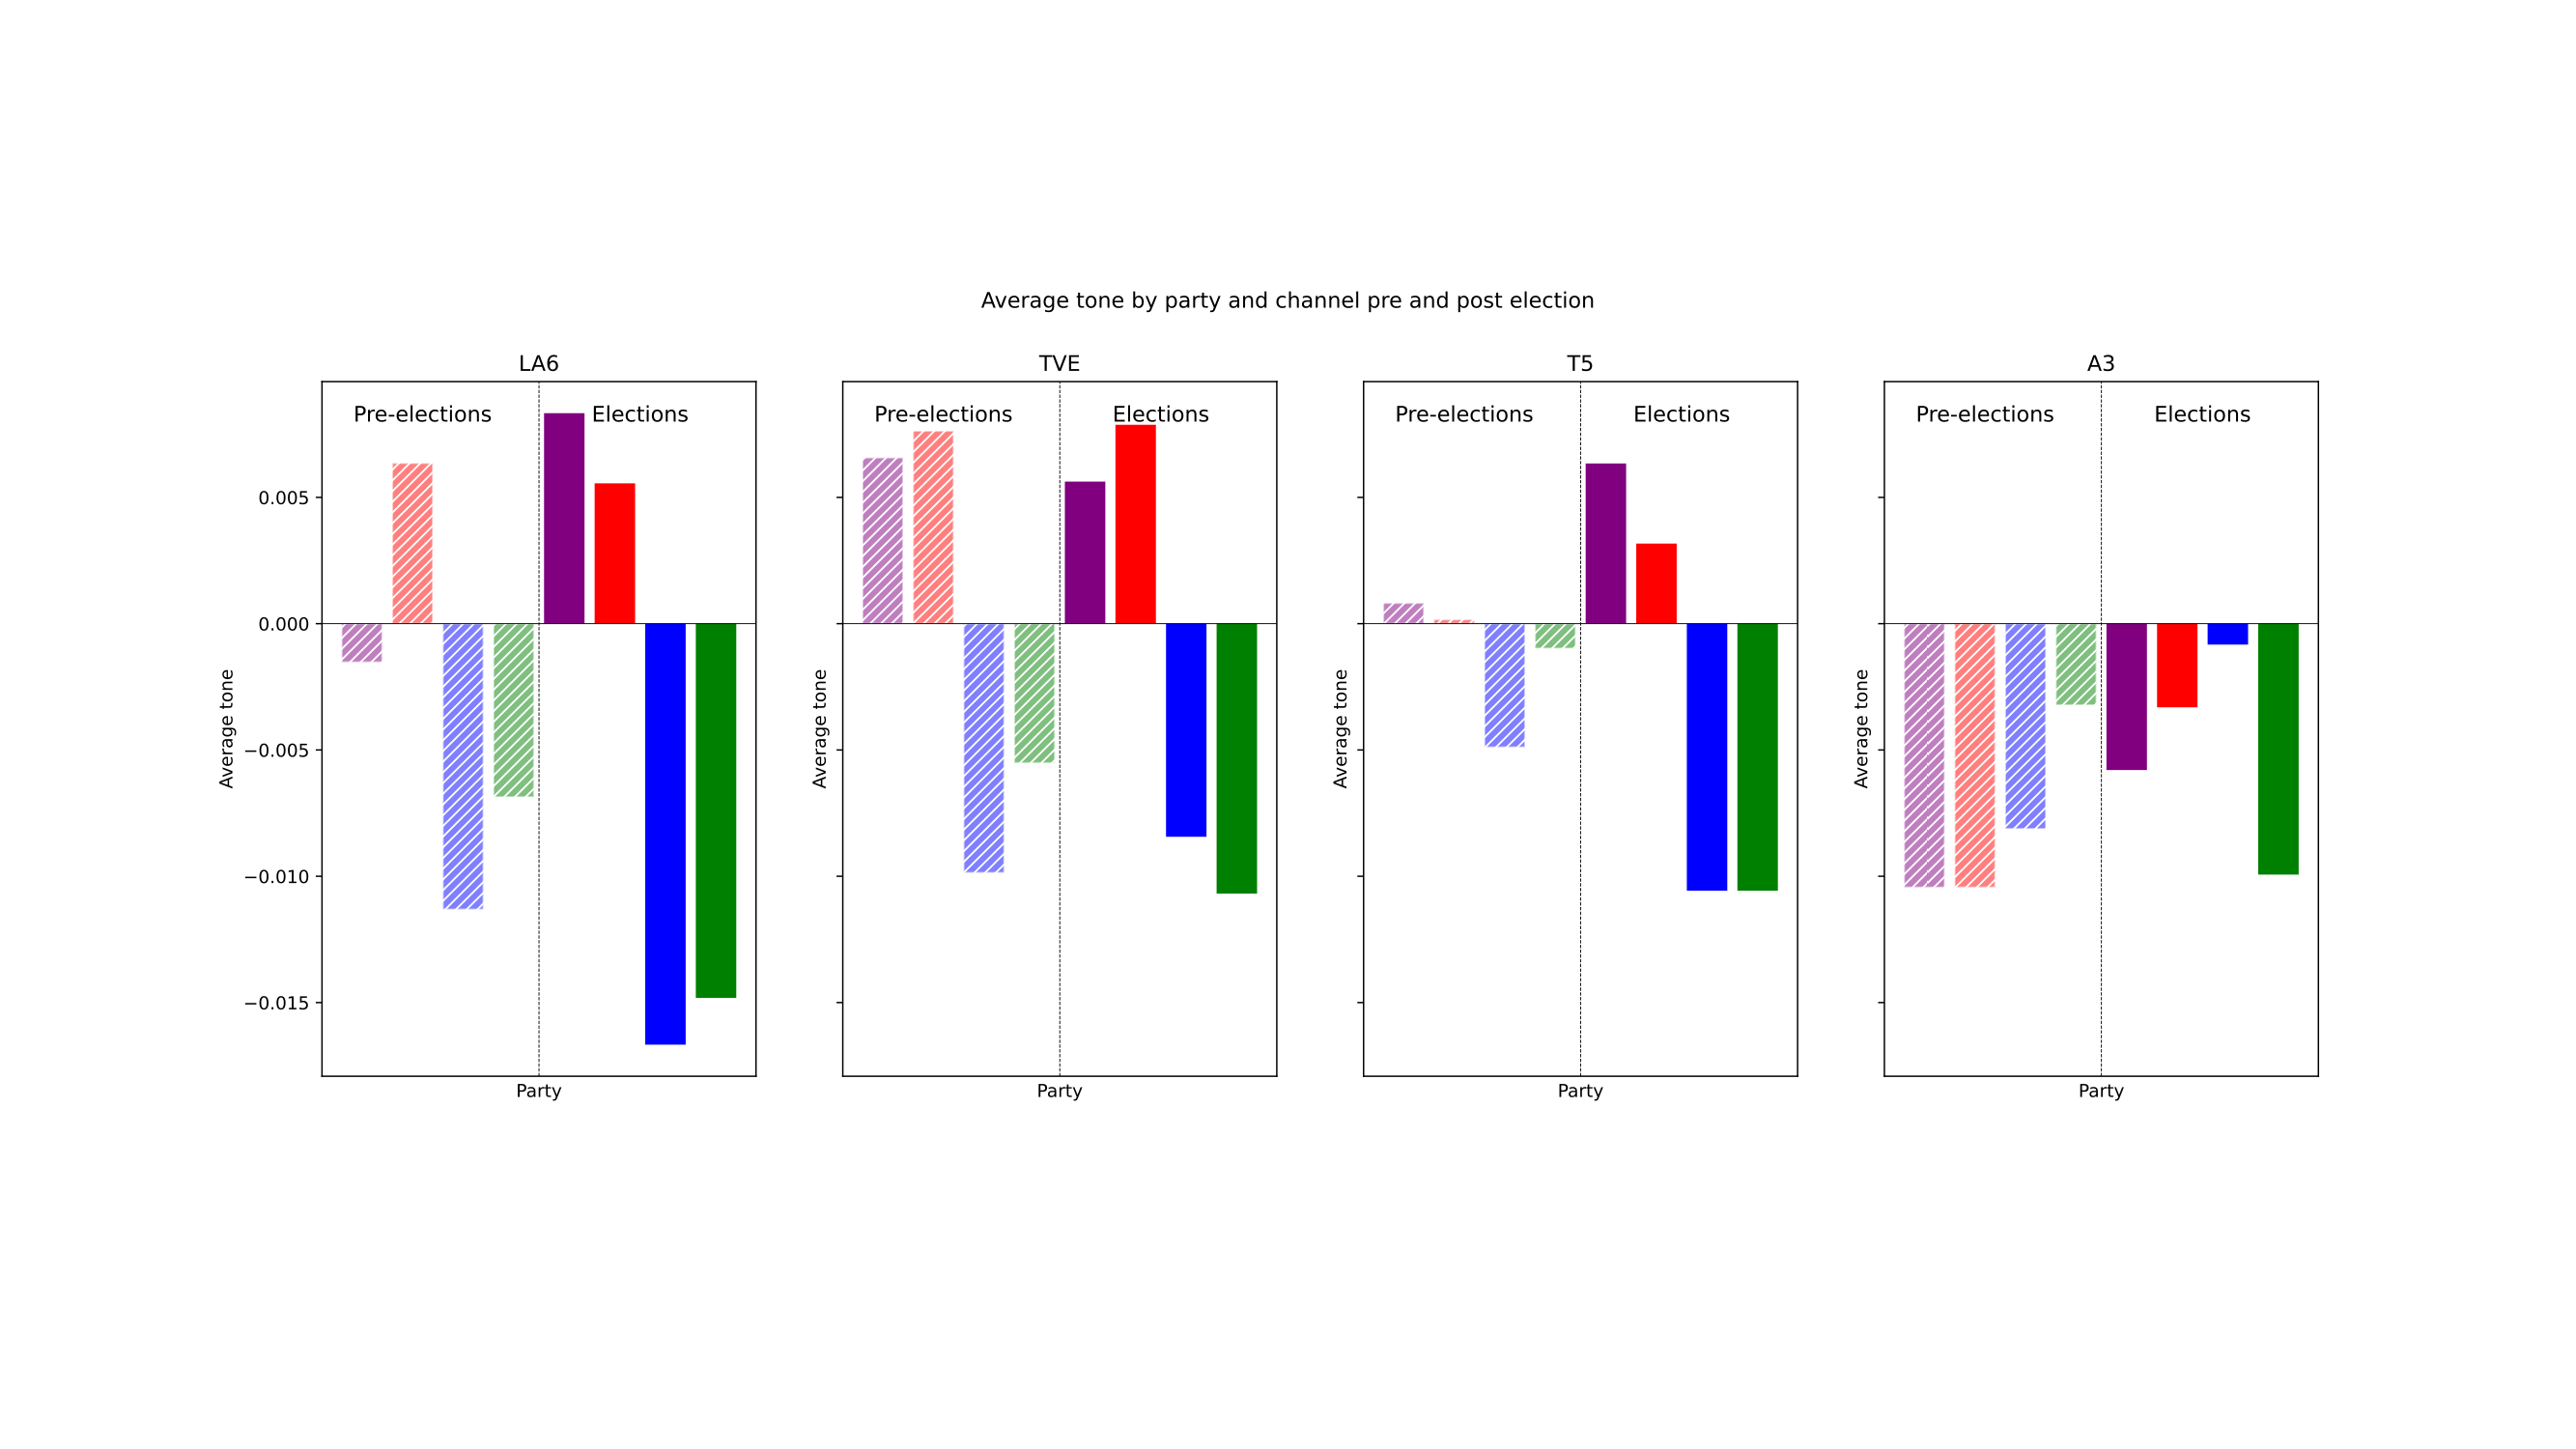
\includegraphics[width=130mm]{figures/average_tone_pre_post_election}
		\caption*{\small \textit{Note:} The figure shows the relative tone calculated as the average sentiment over right and left parties. The vertical dashed line delimits results off and during campaign periods, respectively. }
		\label{fig:tone2}
	\end{figure}
	
	
	
	

	
	
	
	
	\begin{figure}[!htb]
		\caption{Decomposition of Tone across Channels and Parties pre and during Campaign }
		\centering
		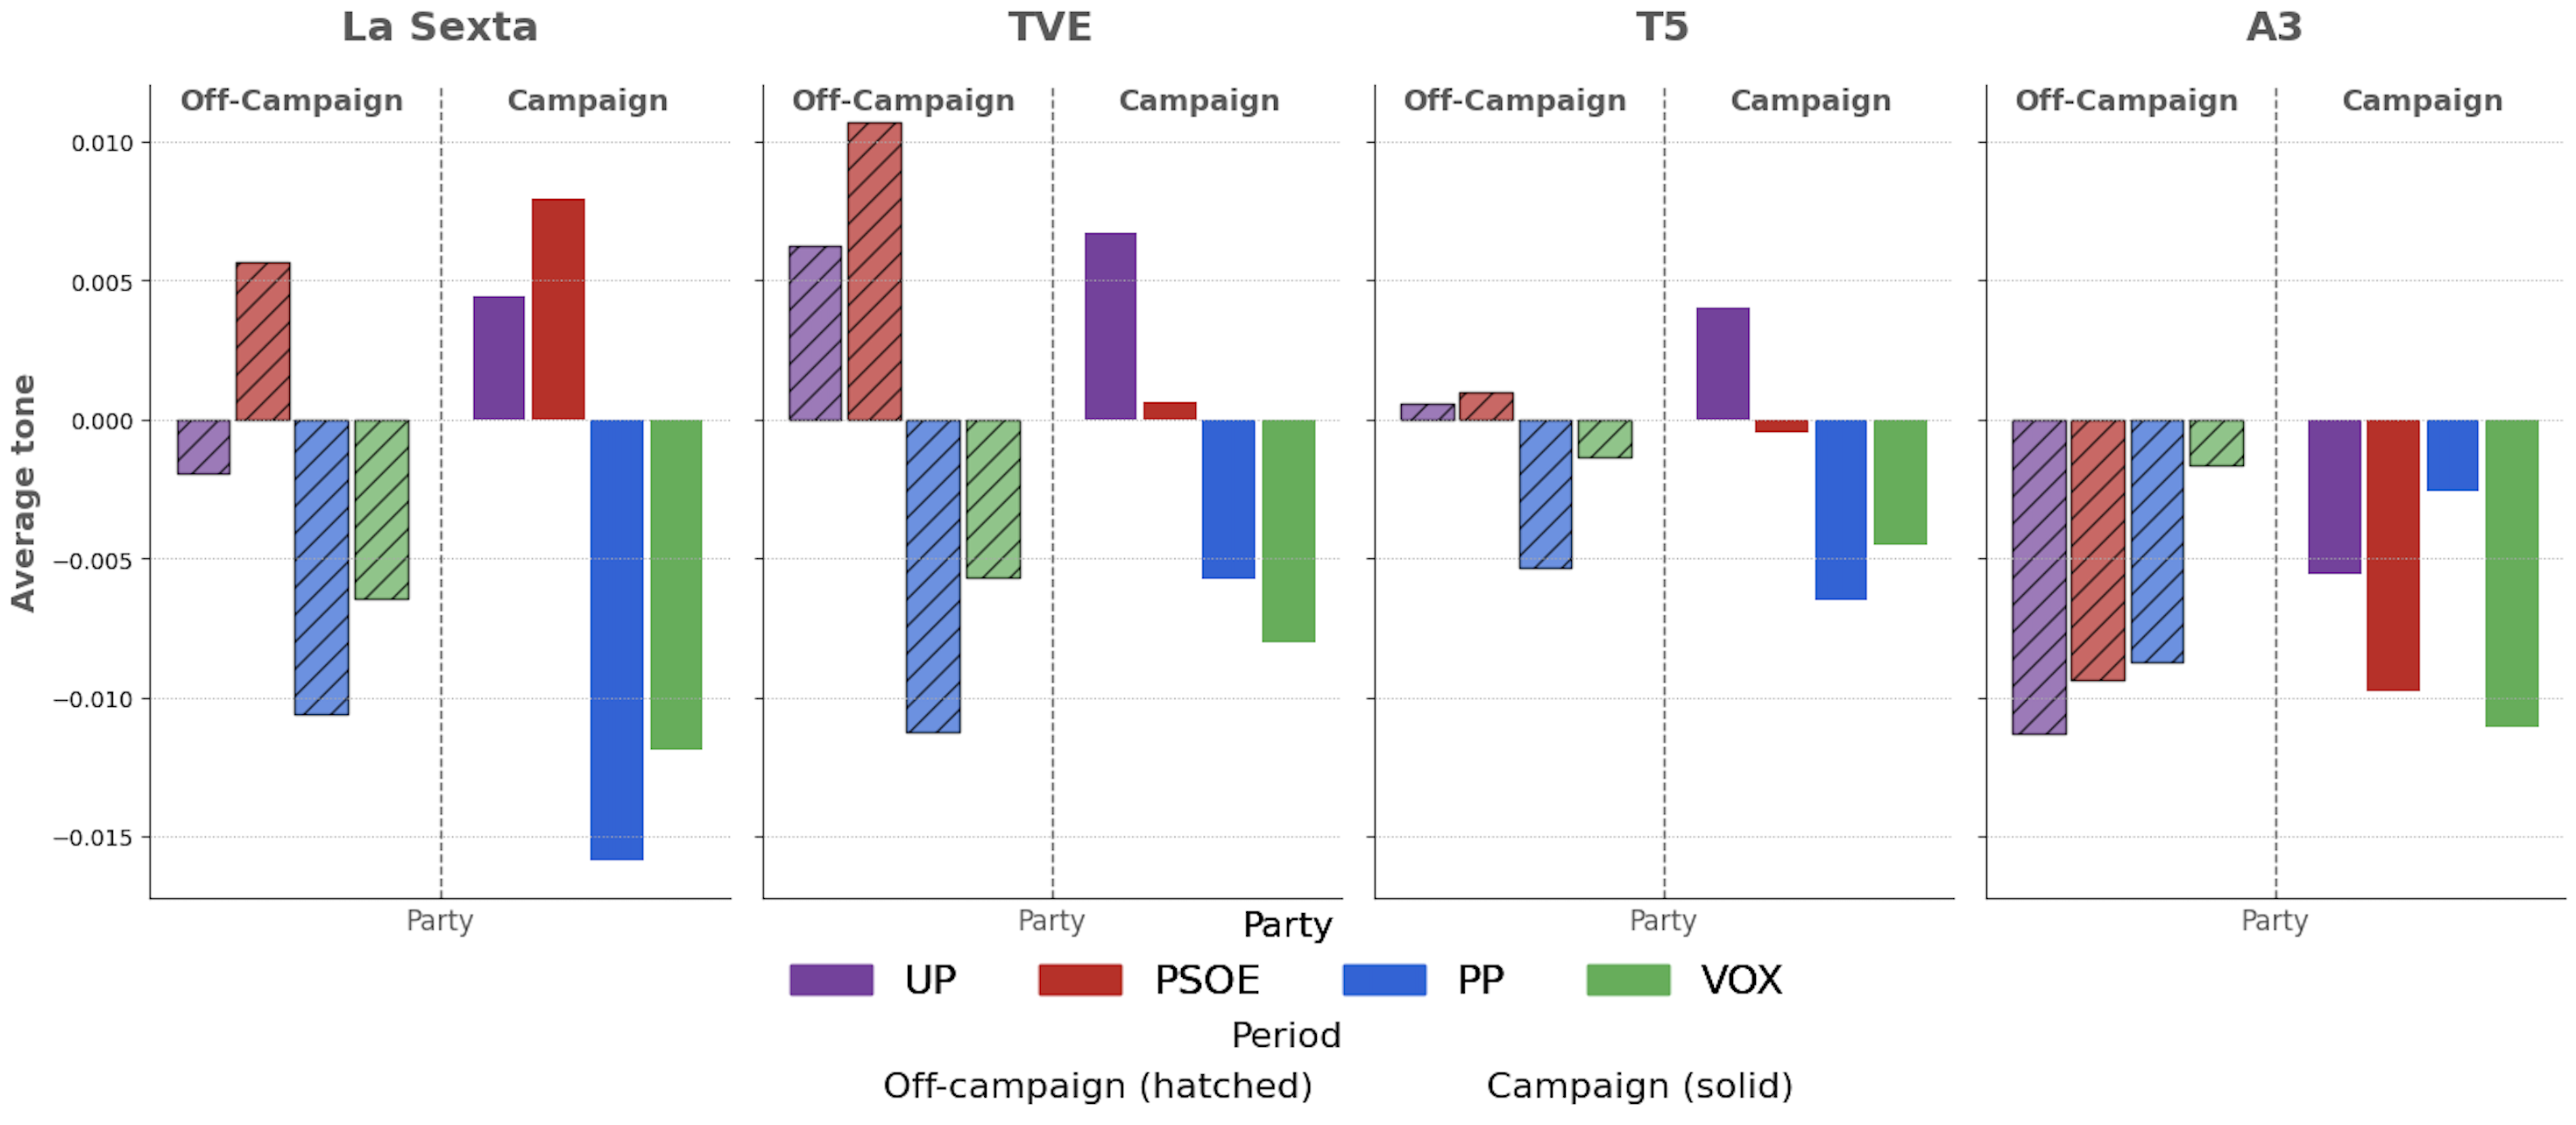
\includegraphics[width=150mm]{figures/average_tone_pre_post_election_party.png}
		\caption*{\small \textit{Note:} The figure shows the relative tone calculated as the average sentiment over each political party. The vertical dashed line delimits results off and during campaign periods, respectively. }
		\label{fig:tone_by_party}
	\end{figure}
	
	
	
	
	\begin{figure}[!htb]
		\caption{TV Audience over Time}
		\centering
		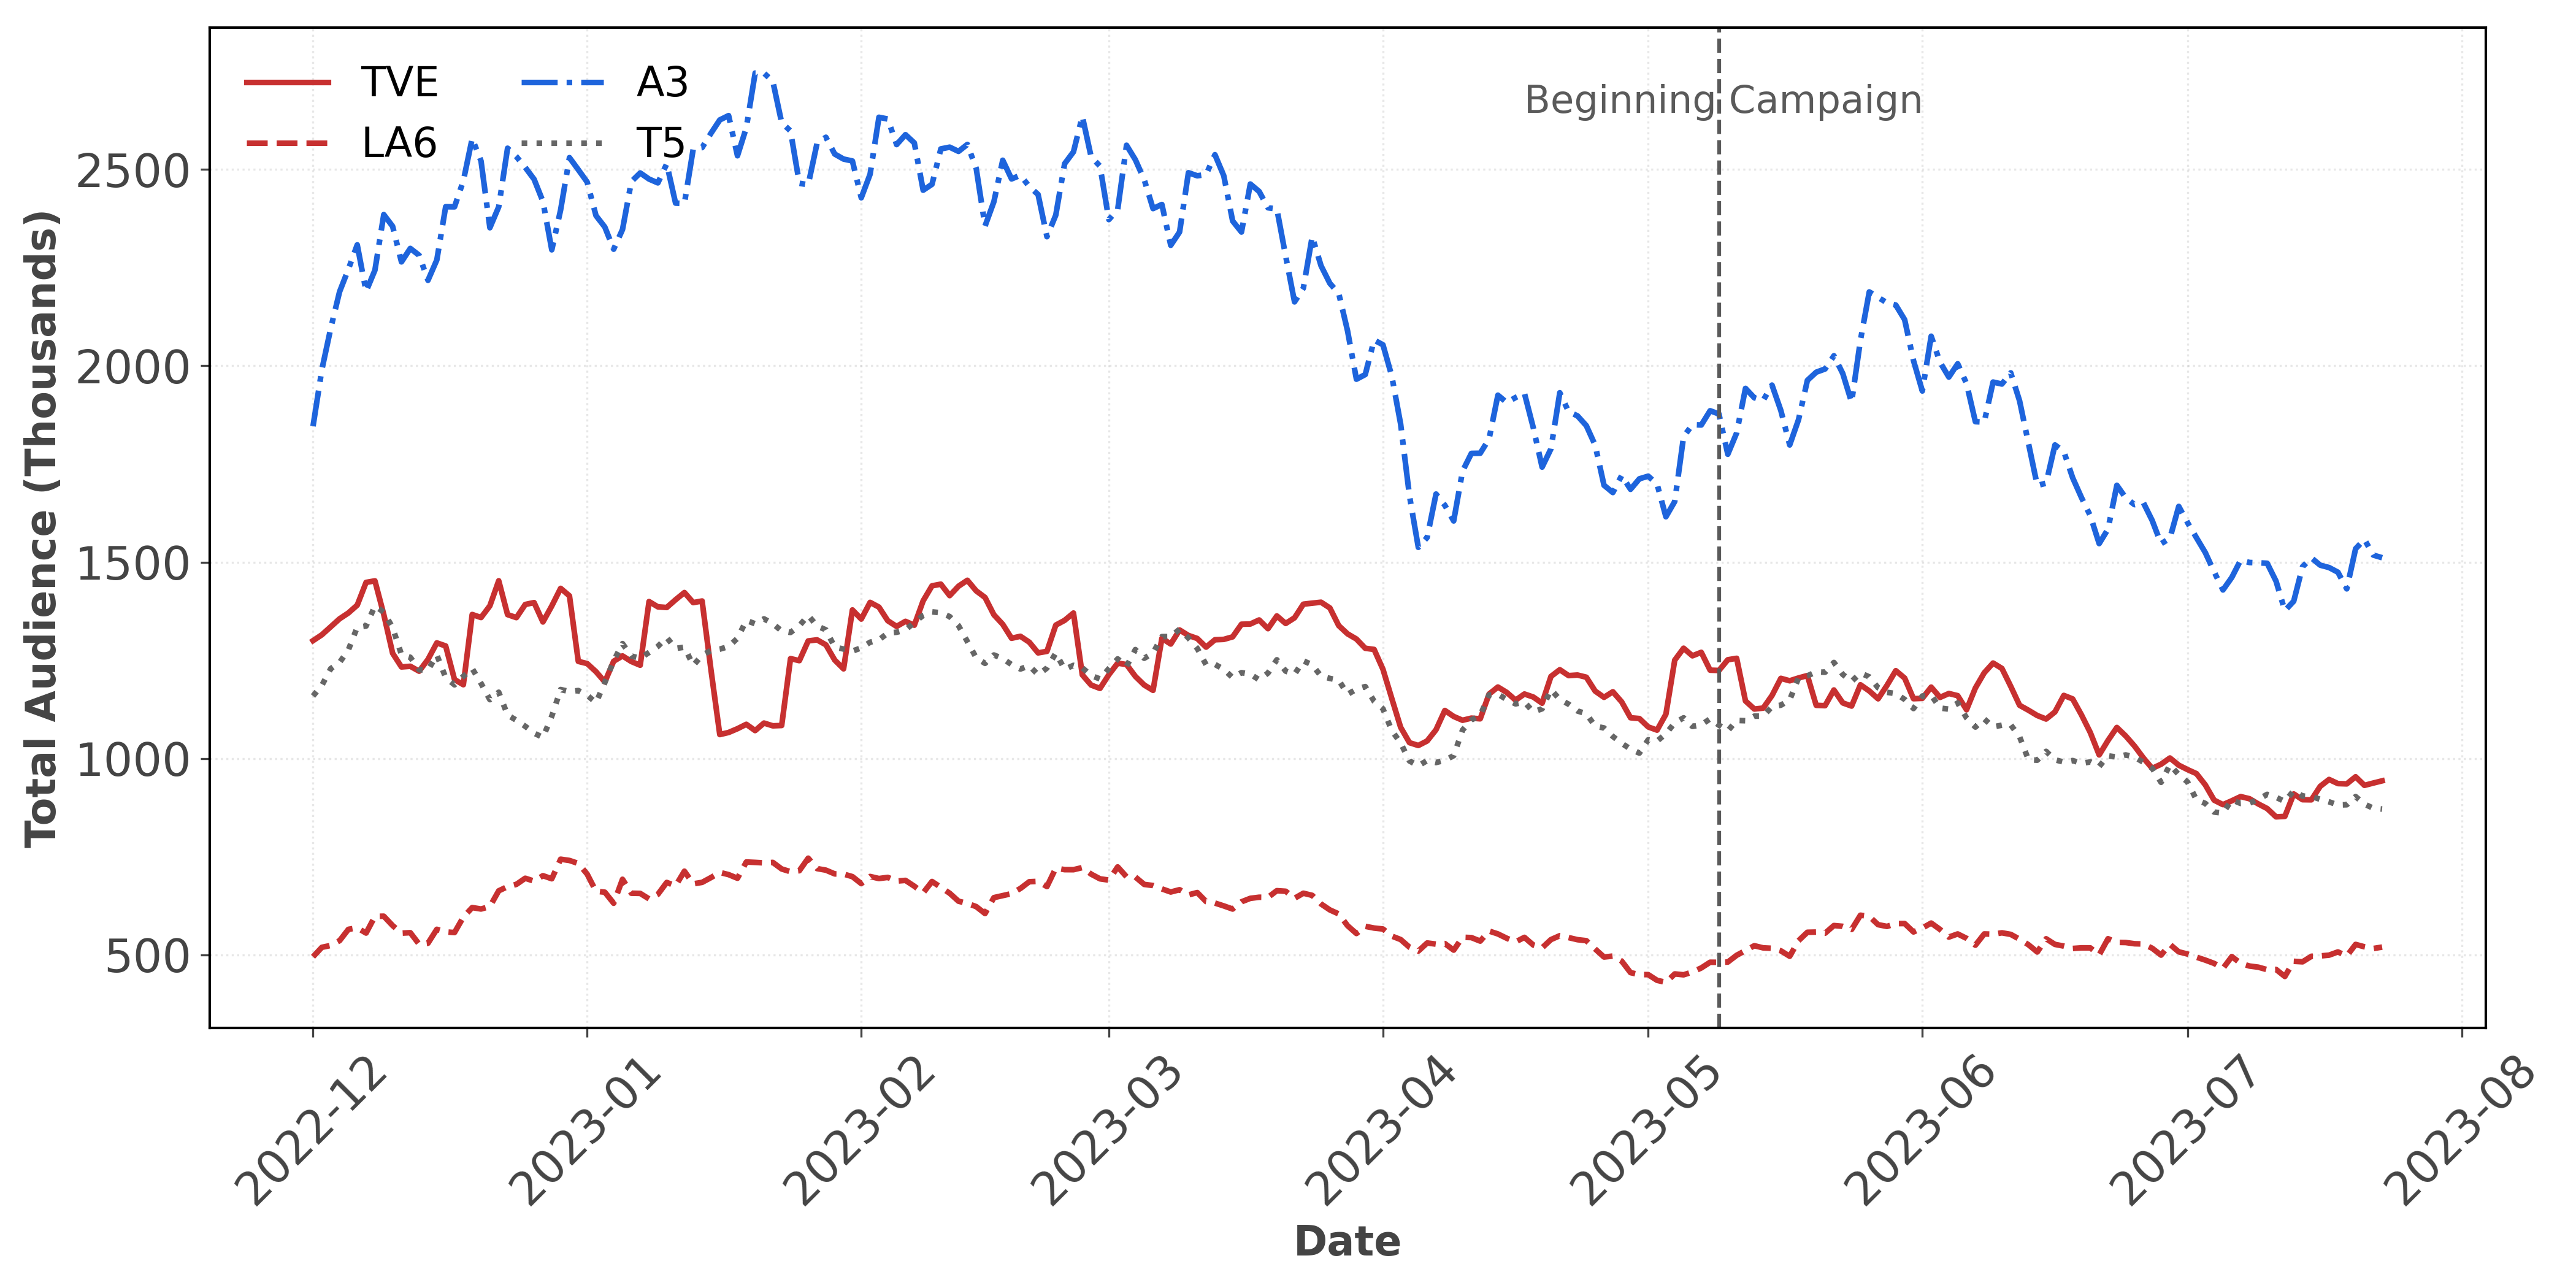
\includegraphics[width=150mm]{figures/tv_audience_total}
		\caption*{\small \textit{Note:} The figure represents the total audience in thousands of viewers for TV outlets. All series are smoothed using a centered rolling mean with a 9-day window.}
		\label{fig:audience_total}
	\end{figure}
	
	

	
	
		\begin{figure}[!htb]
		\caption{Evolution of the Political Coverage by Outlet}
		\centering
		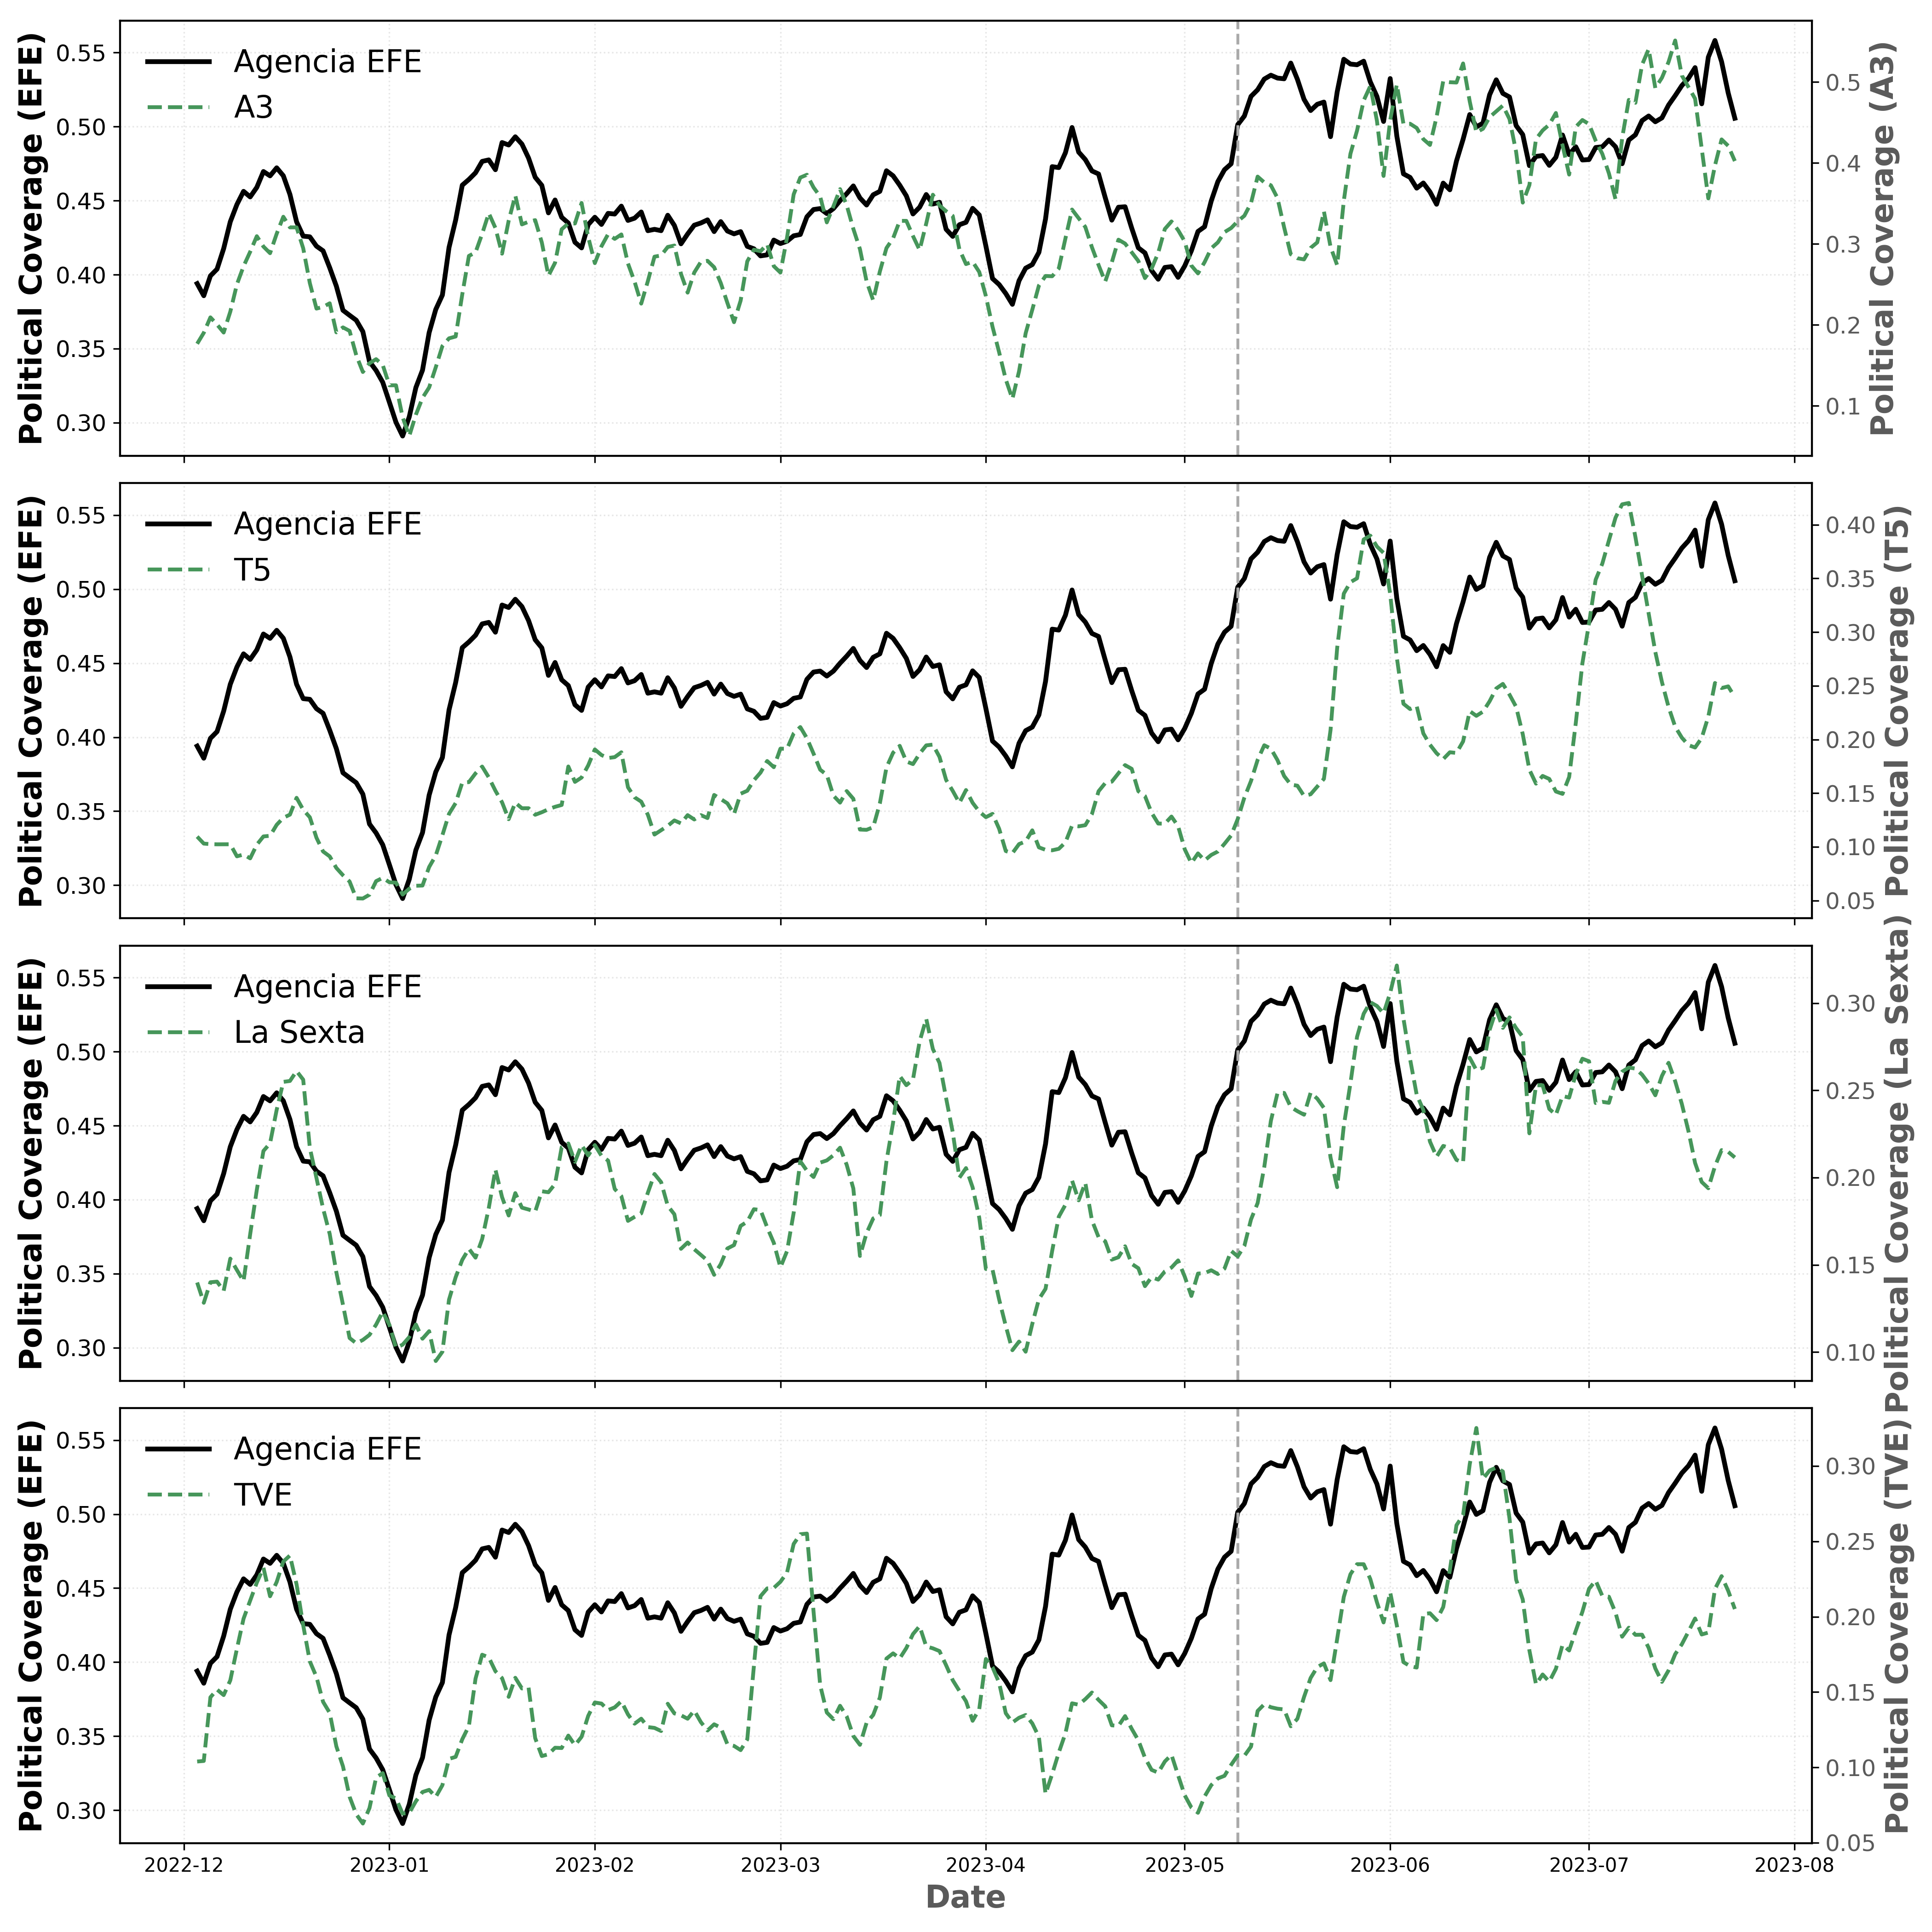
\includegraphics[width=150mm]{figures/tv_vs_efe_political_by_channel}
		\caption*{\small \textit{Note:}The figure represents the smoothed time series of the political coverage for TV channels (right y-axis) and the analogous formula for  EFE (solid) on the left axis. The right axis represents the proportion of political minutes of the outlets. The right axis represents the proportion of political stories.   All series are smoothed using a centered rolling mean with a 9-day window.}
		\label{fig:political_by_channel}
	\end{figure}
	
	
	\begin{figure}[!htb]
		\caption{Evolution of the Ideological Index by Outlet}
		\centering
		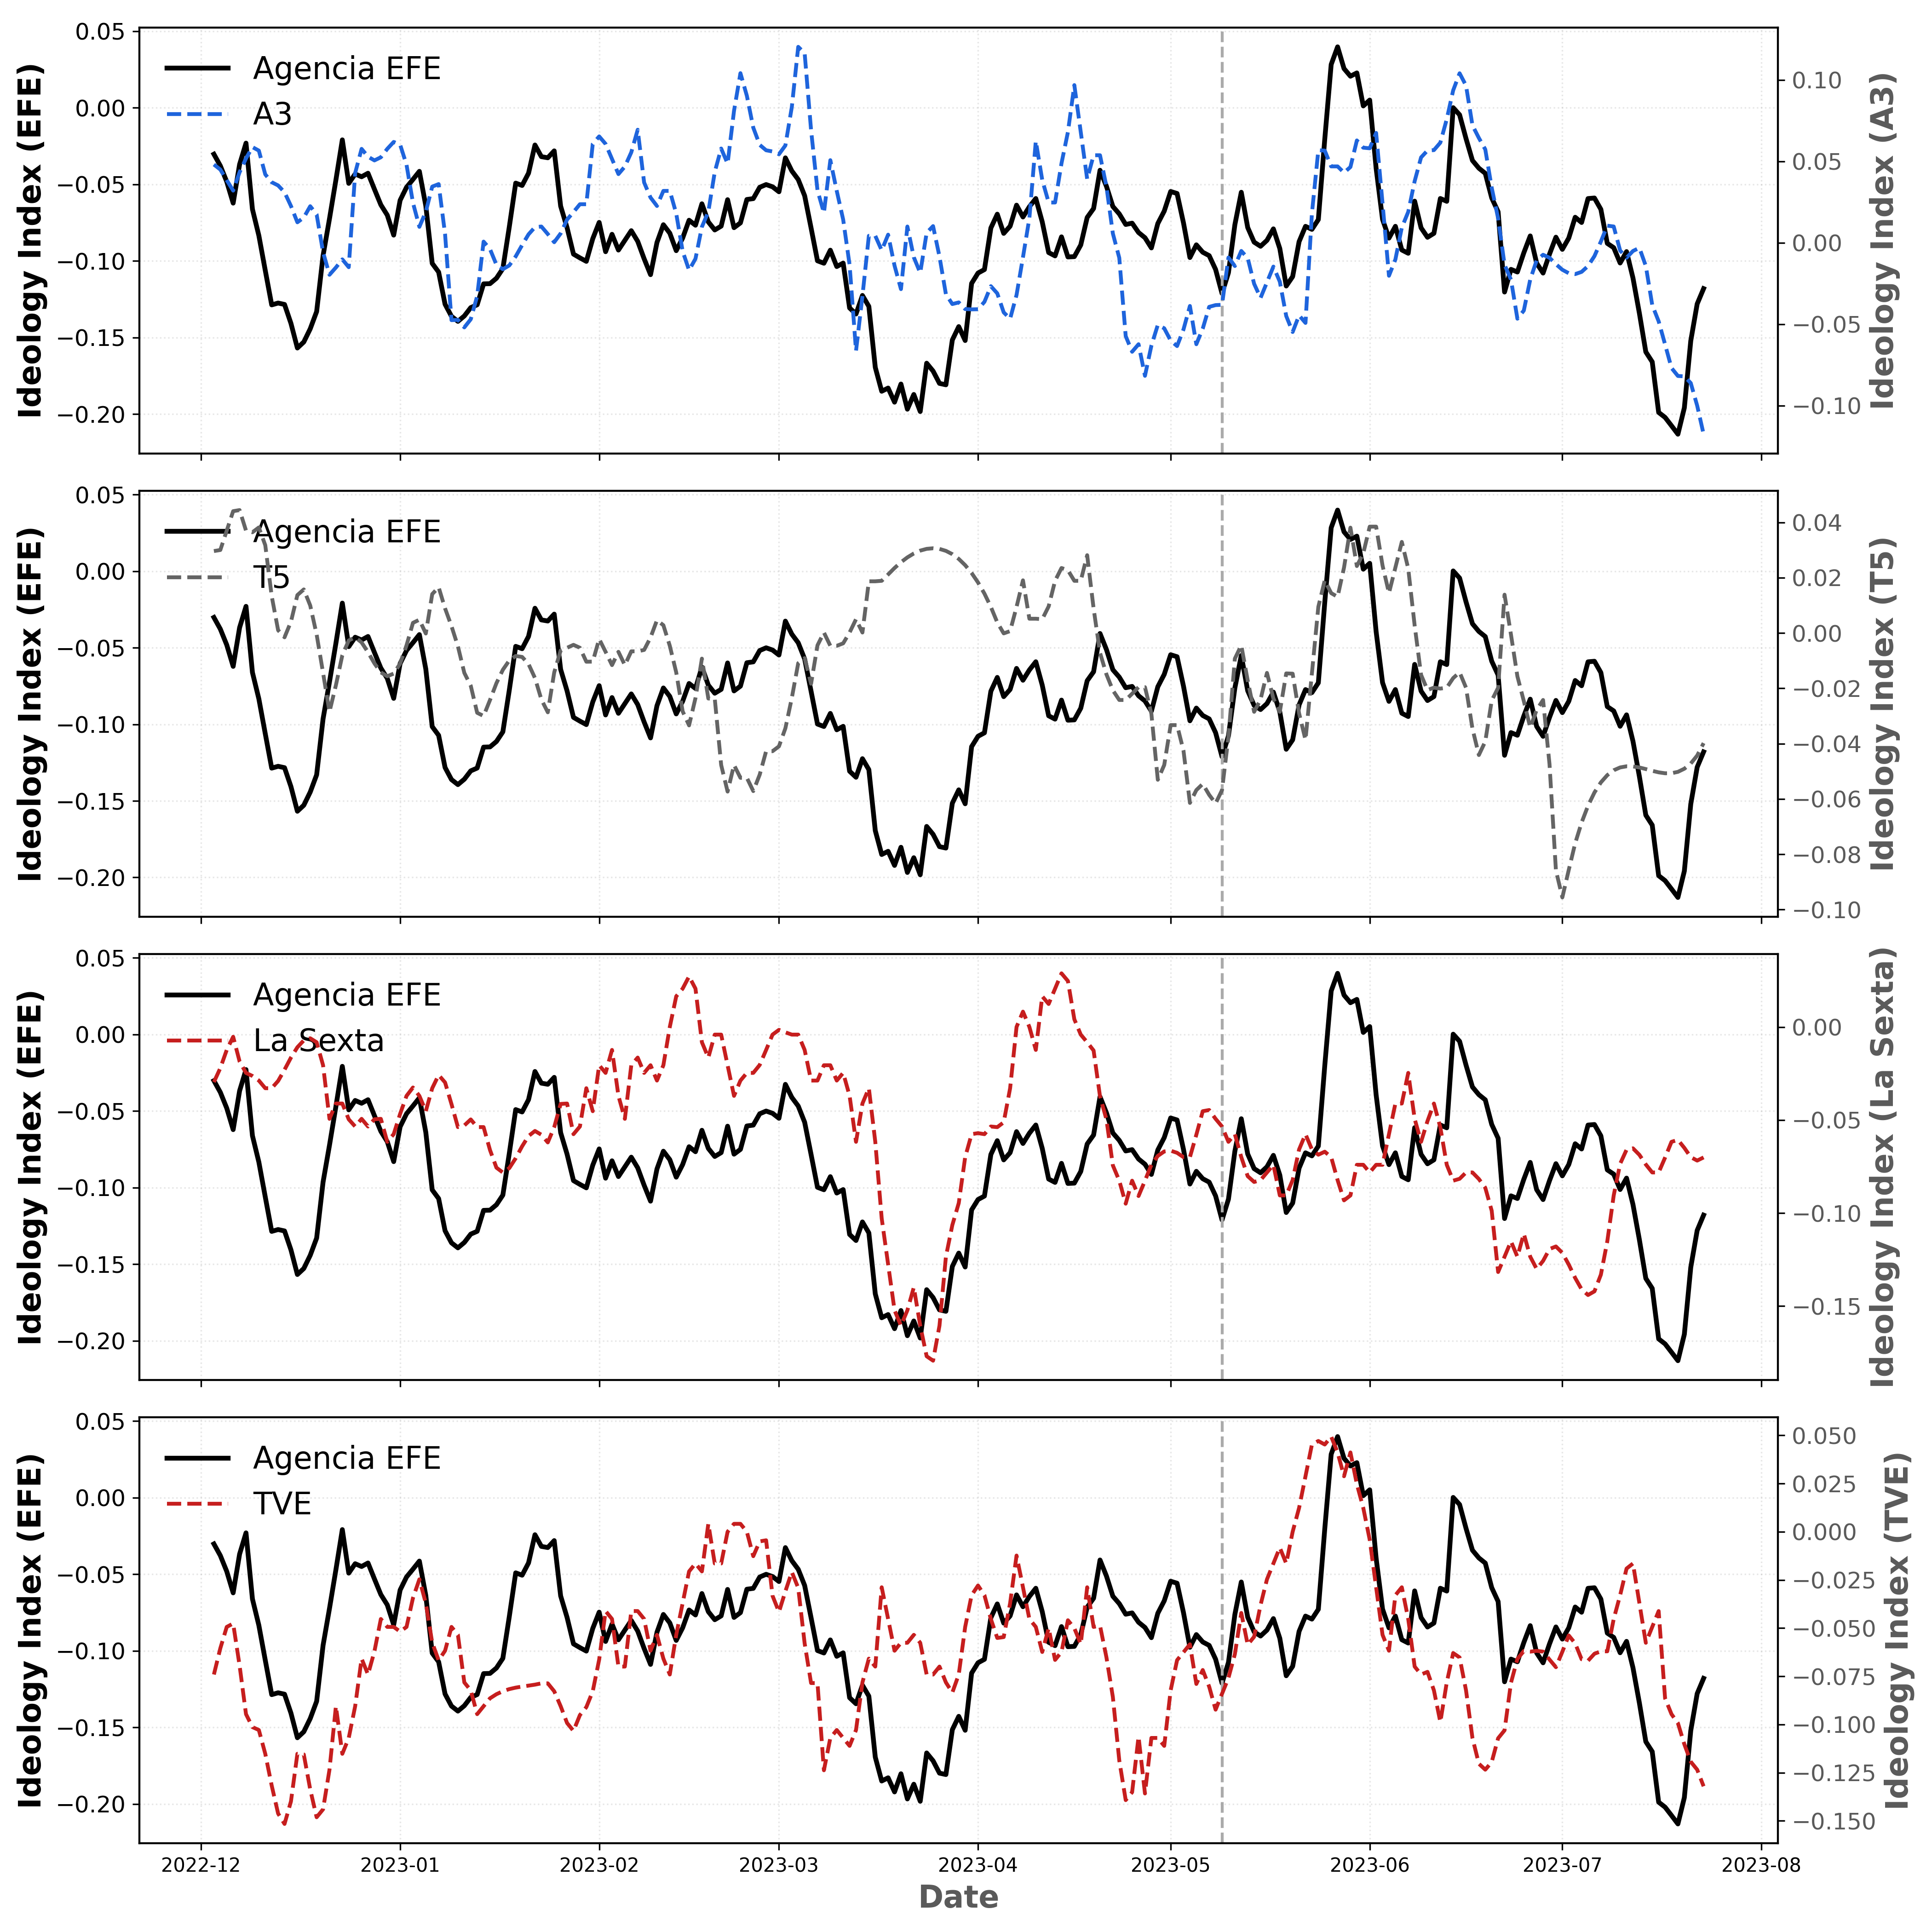
\includegraphics[width=150mm]{figures/tv_vs_efe_net_diff_by_channel}
		\caption*{\small \textit{Note:}The figure represents the smoothed time series of the ideology index in Equation \eqref{eq:ideo_index} for TV channels (right y-axis) and the analogous formula for  EFE (solid) on the left axis. The left axis represents the ideological score of the outlets . All series are smoothed using a centered rolling mean with a 9-day window.}
		\label{fig:net_tone_by_channel}
	\end{figure}
	
	
	
	
	\begin{comment}
	
	\begin{figure}[H]
		\centering
		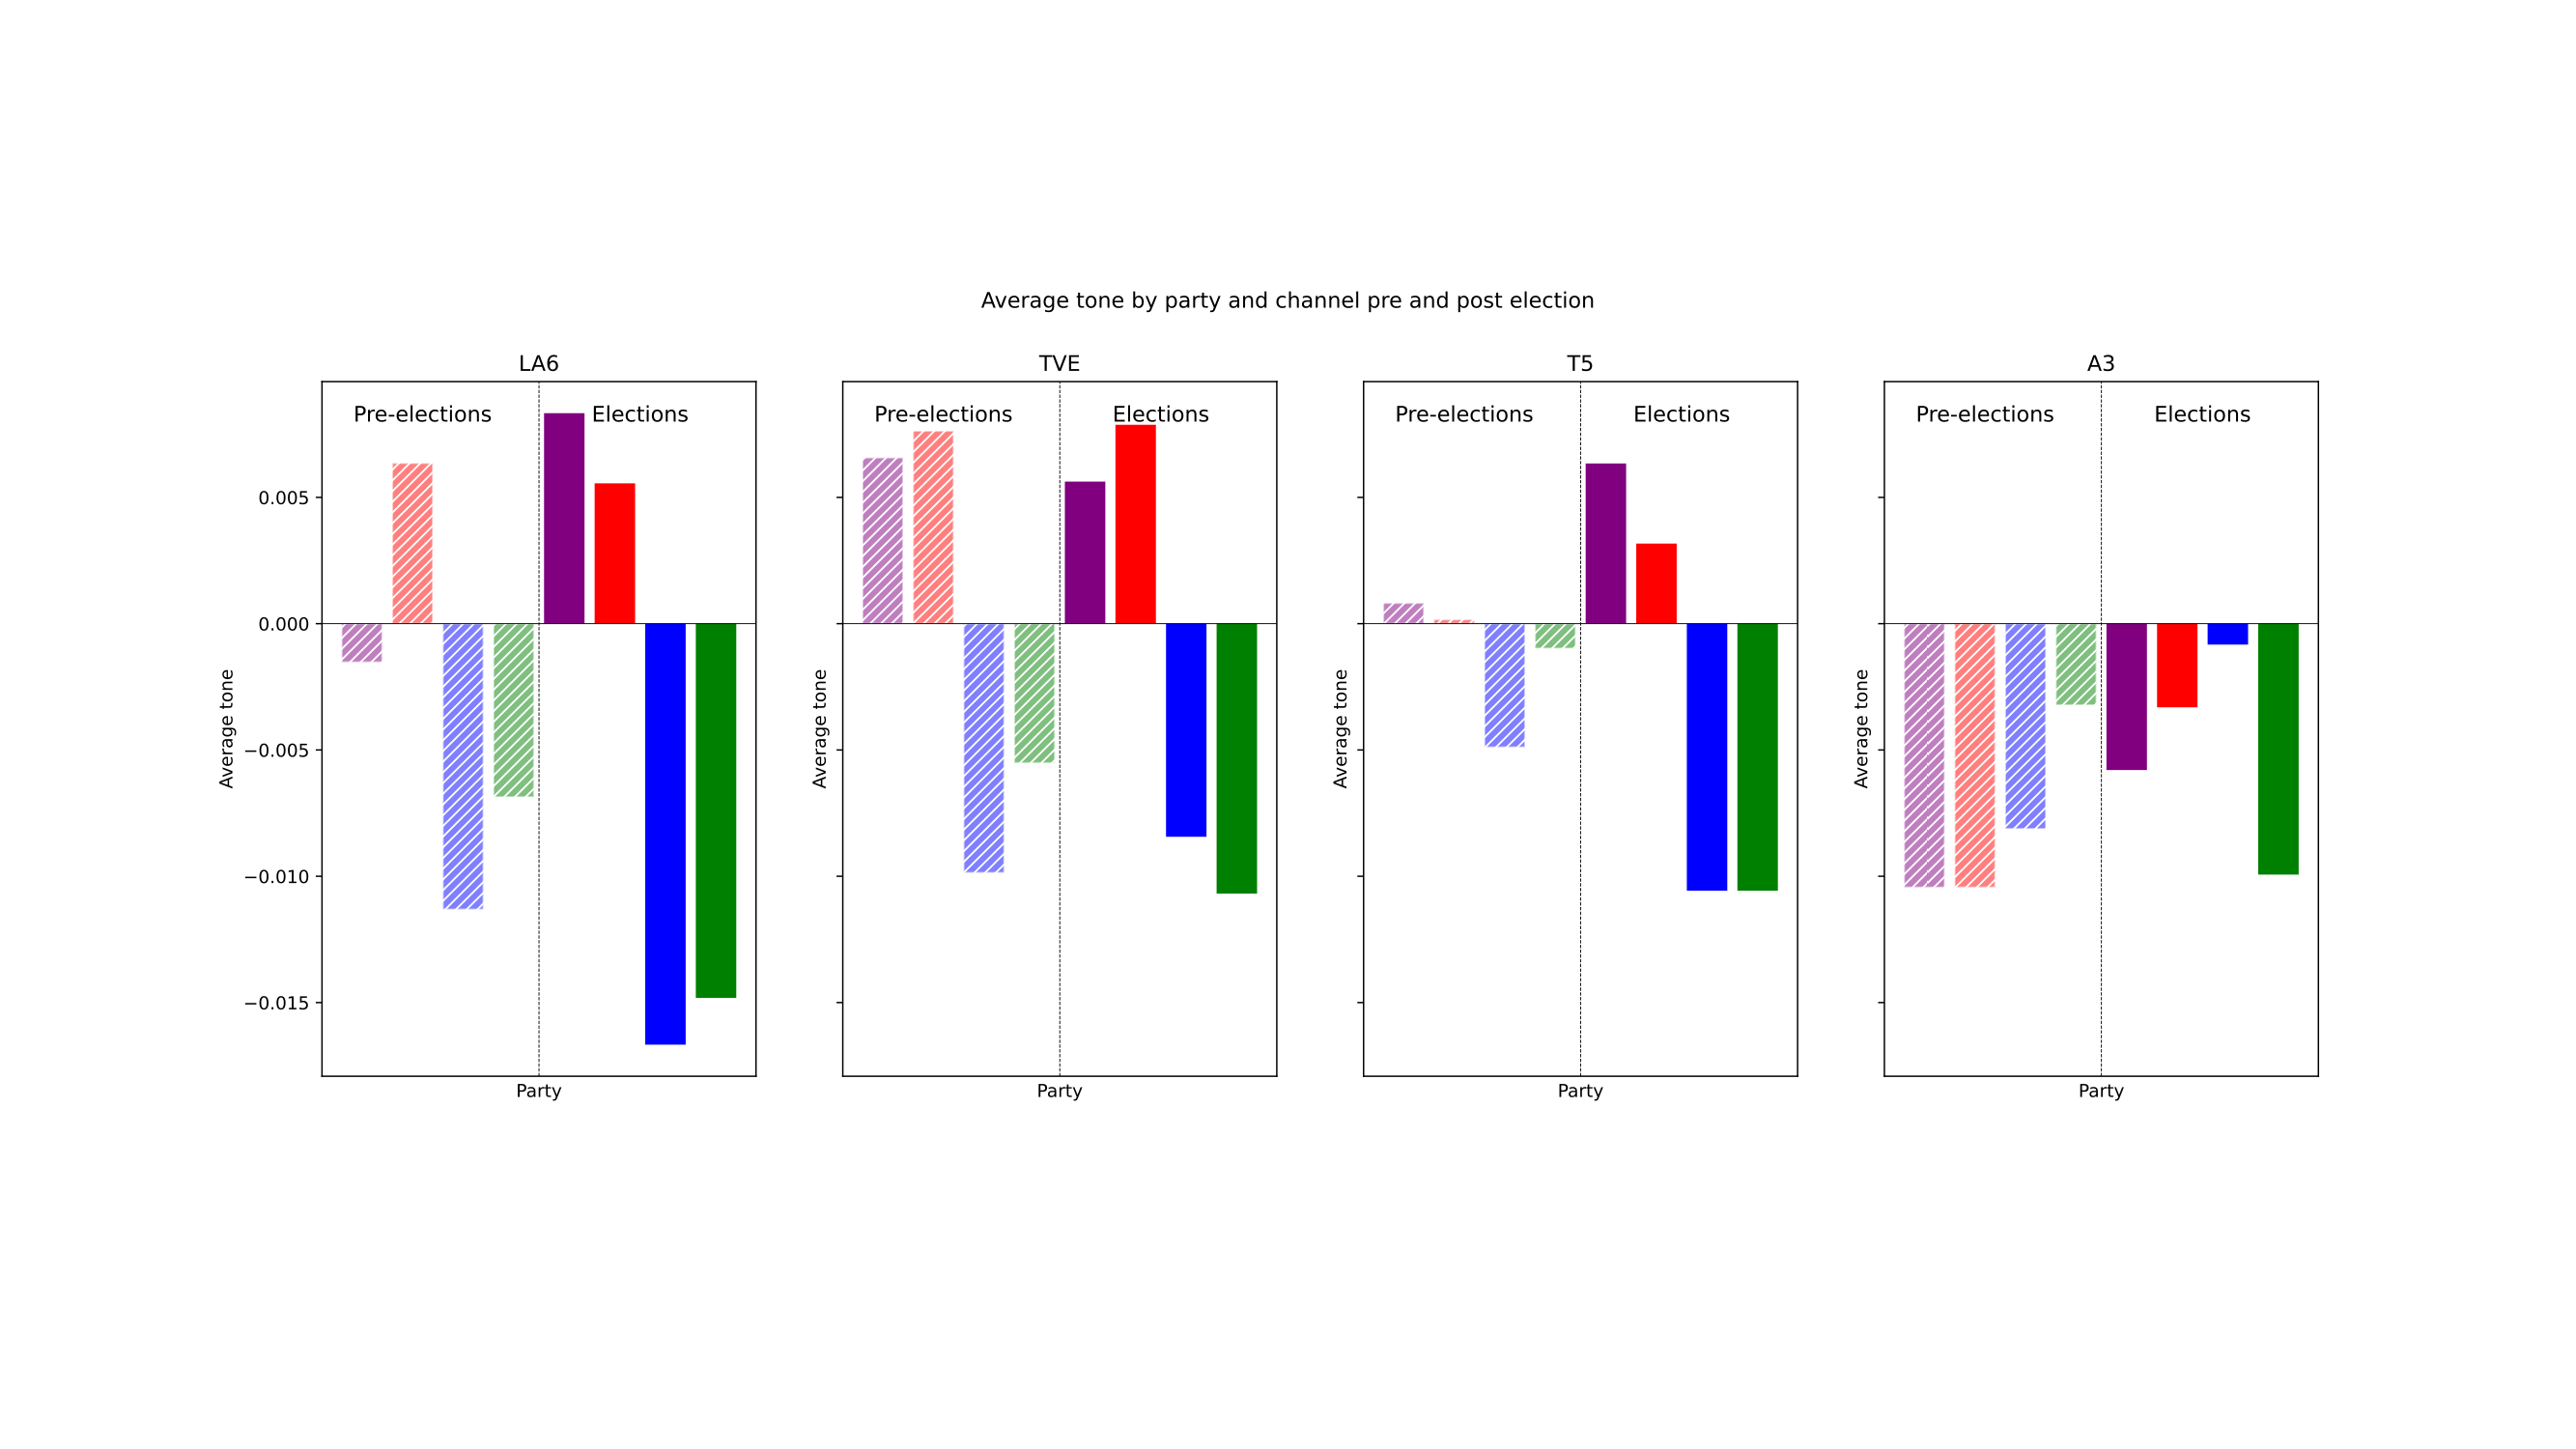
\includegraphics[width=160mm]{figures/average_tone_pre_post_election.png}
		\caption{Average tone for each party and channel pre and during campaign periods}
		\label{fig:party_decomposition}
\end{figure}

		\begin{figure}[h!]
		\caption{Trade-offs in the Model}
		\label{fig:diagram}
		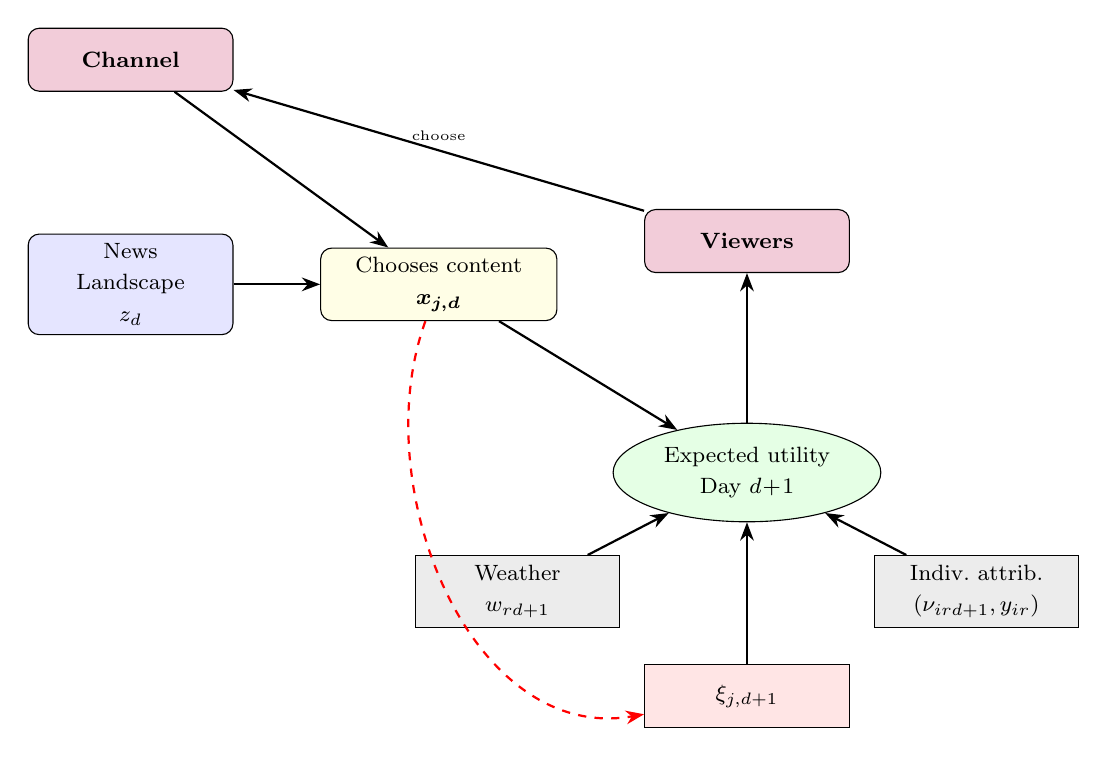
\begin{tikzpicture}[
			inst/.style   ={rectangle, draw, fill=blue!10,  rounded corners, align=center,
				minimum width=2.6cm, minimum height=0.8cm},
			decision/.style={rectangle, draw, fill=yellow!10, rounded corners, align=center,
				minimum width=3.0cm, minimum height=0.9cm},
			util/.style   ={ellipse,   draw, fill=green!10,  align=center,
				minimum width=3.4cm, minimum height=1.0cm},
			shock/.style  ={rectangle, draw, fill=red!10,   align=center,
				minimum width=2.6cm, minimum height=0.8cm},
			exo/.style    ={rectangle, draw, fill=gray!15,  align=center,
				minimum width=2.6cm, minimum height=0.8cm},
			actor/.style  ={rectangle, draw, fill=purple!20, rounded corners, align=center,
				minimum width=2.6cm, minimum height=0.8cm},
			flow/.style   ={-Stealth, thick},
			feed/.style   ={dashed,-Stealth, thick, red},
			node distance = 1.8cm and 1.1cm,
			font=\footnotesize
			]
			% -------- DAY d (supply) ---------
			\node[inst]                    (news)   {News\\Landscape\\$z_{d}$};
			\node[actor, above=of news]    (channel) {\textbf{Channel}};
			
			\node[decision, right=of news] (x)      {Chooses content\\$\bm{x_{j,d}}$};
			
			% -------- DAY d+1 (demand) ------
			\node[actor, right=of x, yshift=0.55cm] (viewer) {\textbf{Viewers}};
			
			\node[util,  below=of viewer, yshift=-0.1cm] (util)
			{Expected utility\\Day $d\!+\!1$};
			\node[shock, below=of util]     (xi)     {$\xi_{j,d+1}$};
			\node[exo,   below left=0.6cm and 0.4cm of util]
			(weather){Weather\\$w_{rd+1}$};
			\node[exo,   below right=0.6cm and 0.4cm of util]
			(prefs)  {Indiv.\ attrib.\\$(\nu_{ird+1},y_{ir})$};
			
			% ---------- flows ---------------
			\draw[flow] (channel) -- (x);
			\draw[flow] (news)    -- (x);
			\draw[flow] (x)       -- (util);
			\draw[flow] (prefs)   -- (util);
			\draw[flow] (weather) -- (util);
			\draw[flow] (xi)      -- (util);
			\draw[flow] (util)    -- (viewer) node[midway,right,font=\tiny]{};
			\draw[flow] (viewer)    -- (channel) node[midway,above,font=\tiny]{choose};
			
			
			% ------ anticipation feedback ---
			\draw[feed] (x) to[out=-110,in=190] node[midway,below,font=\tiny]
			{} (xi);
		\end{tikzpicture}
		\caption*{\small
			\textit{Note:} This diagram illustrates the structure of the model. Solid black arrows indicate causal and temporal dependencies among variables. The red dashed arrow emphasizes the simultaneity problem: content decisions $\bm{x}_{j,d}$ are made with knowledge of the future utility shock $\xi_{j,d+1}$.
		}
		
	\end{figure}
	
		\end{comment}	
	
	\begin{comment}
		content...

	\begin{figure}[ht!]
		\centering
		\caption{Density Estimation for Channels' Ideology (Audience Share)}
		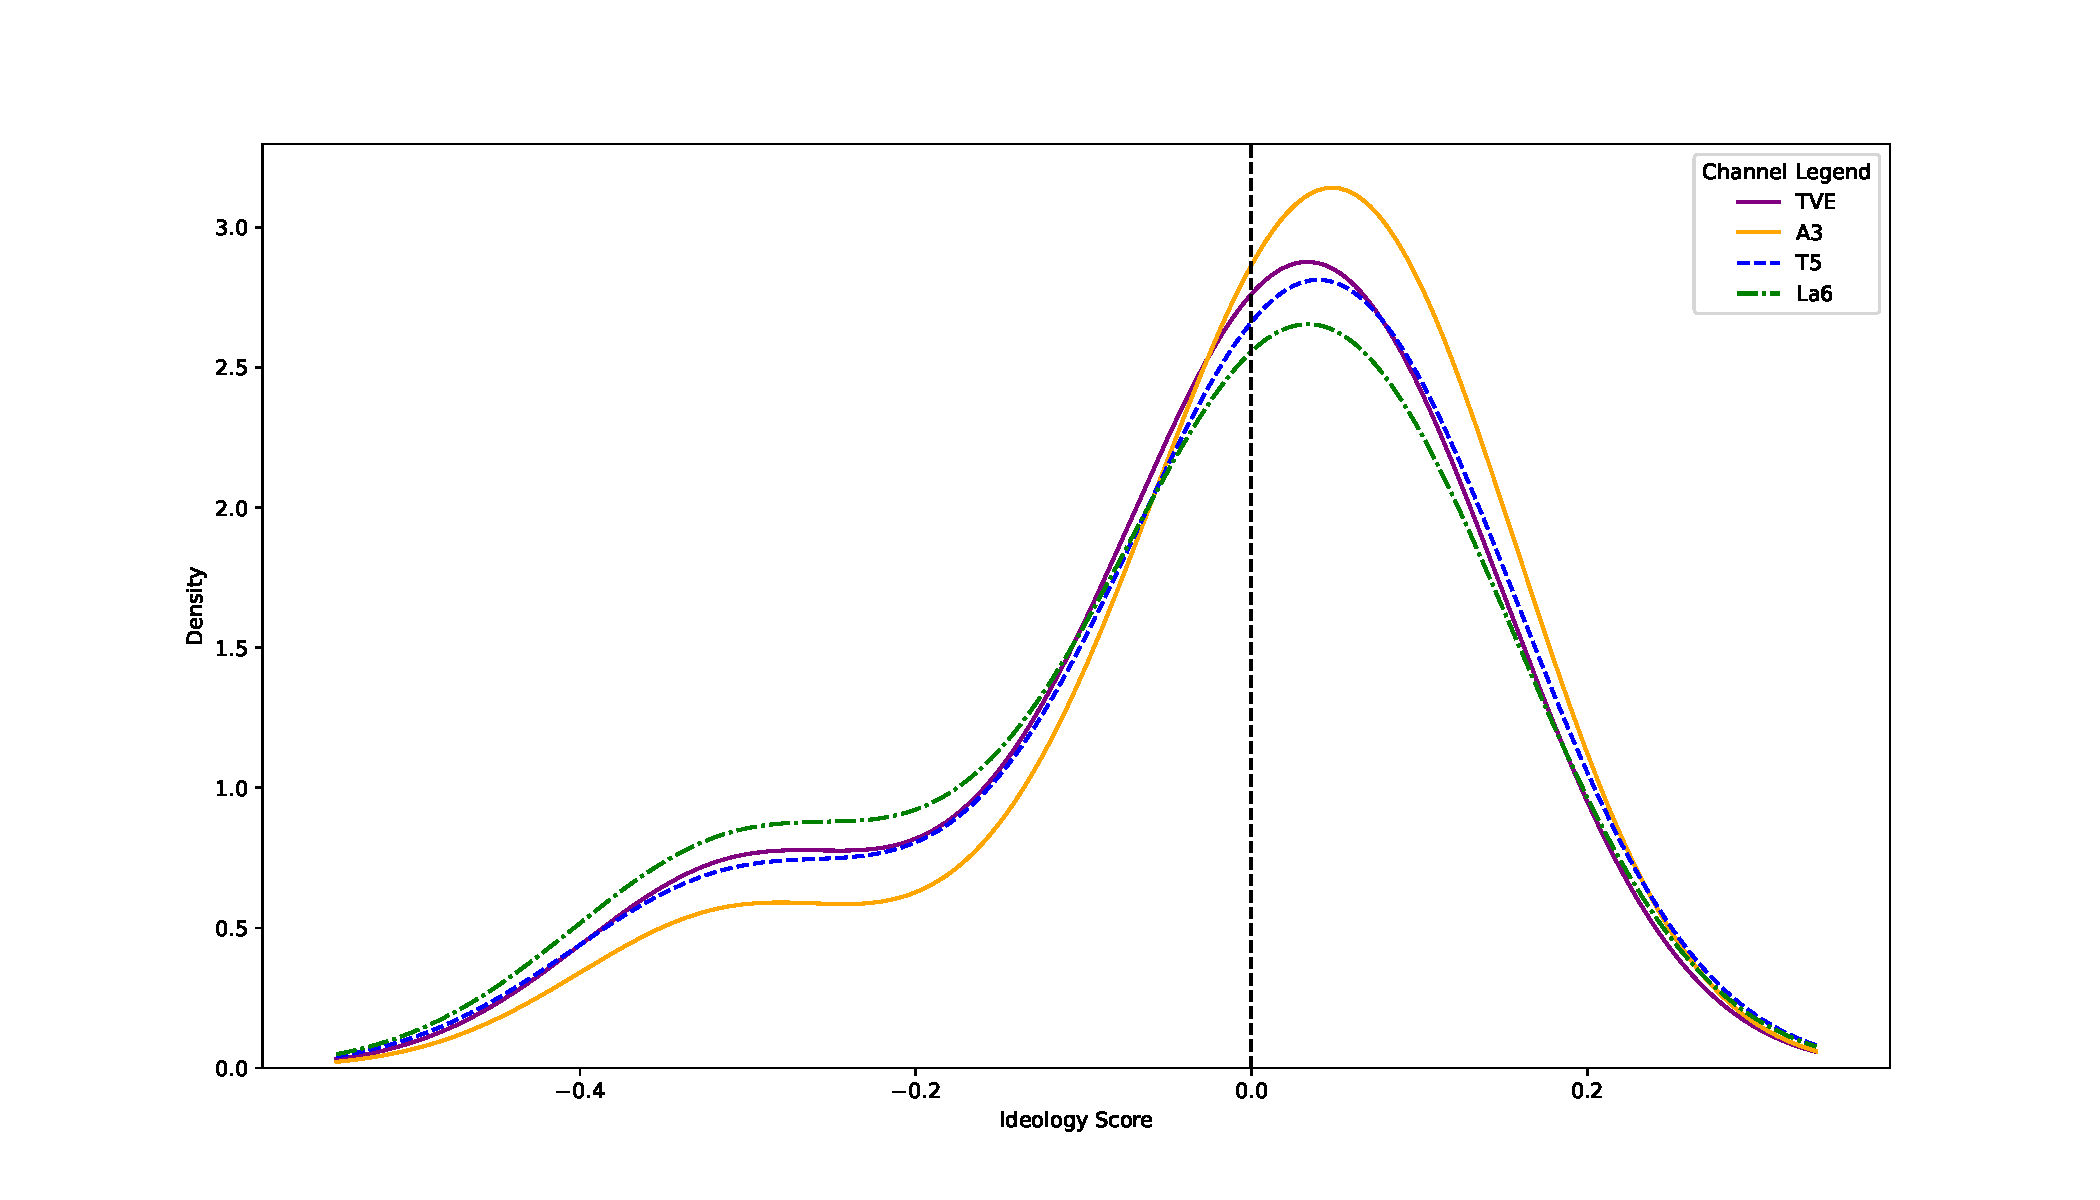
\includegraphics[width=120mm]{figures/channel_ideology_density_python}
		\caption*{\small \textit{Note:} Estimated density of channels' audience ideology. The figure shows a kernel density estimate on the ideology score constructed using survey daa and weighted by channels' share of audience for each autonomous region. }
		\label{fig:density}
	\end{figure}
	
		\end{comment}
		
		\begin{figure}[ht!]
		\centering
		\caption{Added Variable Plots for Production of Political Content (non-parametric fit)}
		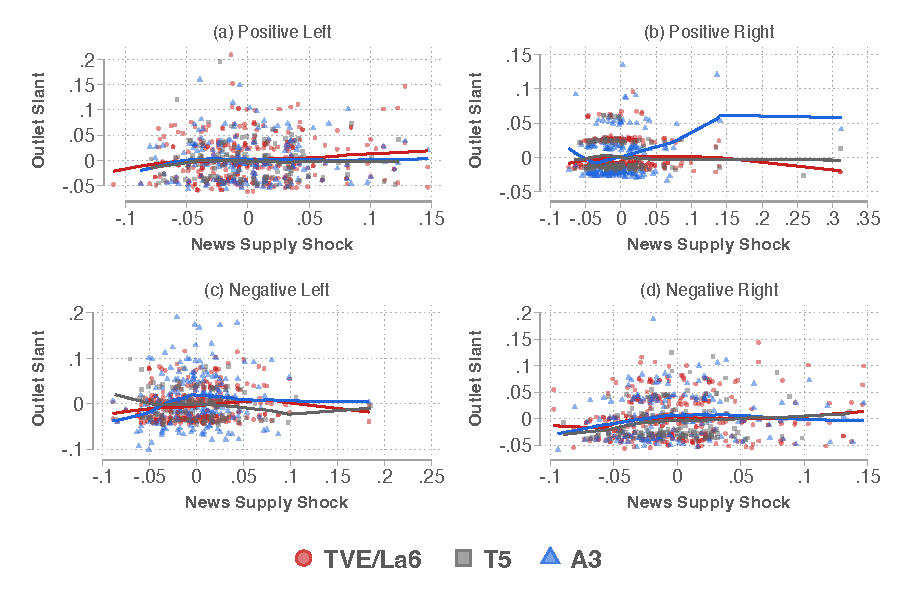
\includegraphics[width=160mm]{figures/fwl_plots_lowess_v2}
		\caption*{\small \textit{Note:} The figure shows the added variable plots from the estimation of Eq. \eqref{eq:first_stage}. The x axis represents $(z_d^{party,+},z_d^{party,-}) $ and the y axis the corresponding  $(x_{jd}^{party,+},x_{jd}^{party,-}) $   . Channels are pooled into left (TVE and La Sexta), middle (T5) and right (A3) for visualization purposes.  }
		\label{fig:fwl_lowess}
	\end{figure}
	

	
	\begin{figure}[!htbp]
		\centering
		\caption{Estimated Elasticities for Left and Right markets off-Campaign}
		\label{fig:elasticities_pre}
		\vspace{0.5em} % space between caption and figures
		
		\begin{minipage}{0.45\textwidth}
			\centering
			\textbf{(a)} Left Markets\\
			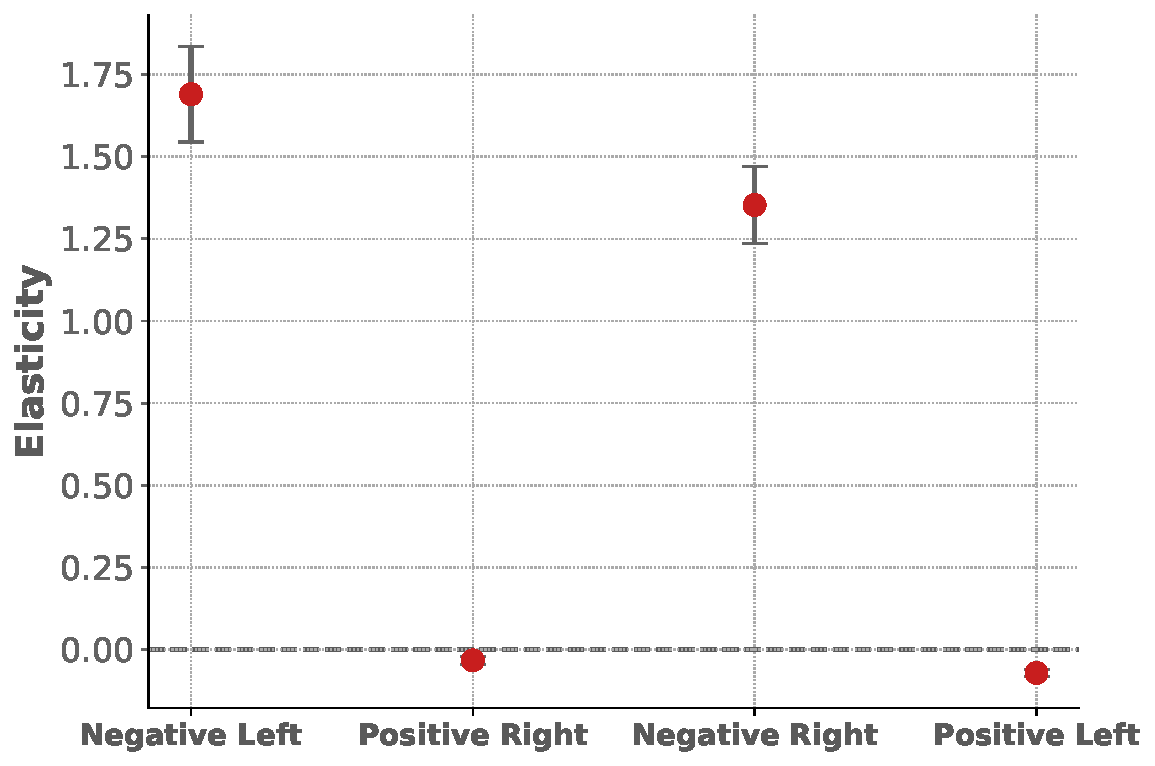
\includegraphics[width=\linewidth]{figures/elasticities_left_pre}
			%		\label{fig:2figsA}
		\end{minipage}
		\hfill
		\begin{minipage}{0.45\textwidth}
			\centering
			\vspace{1.5em}
			\textbf{(b)} Right Markets \\
			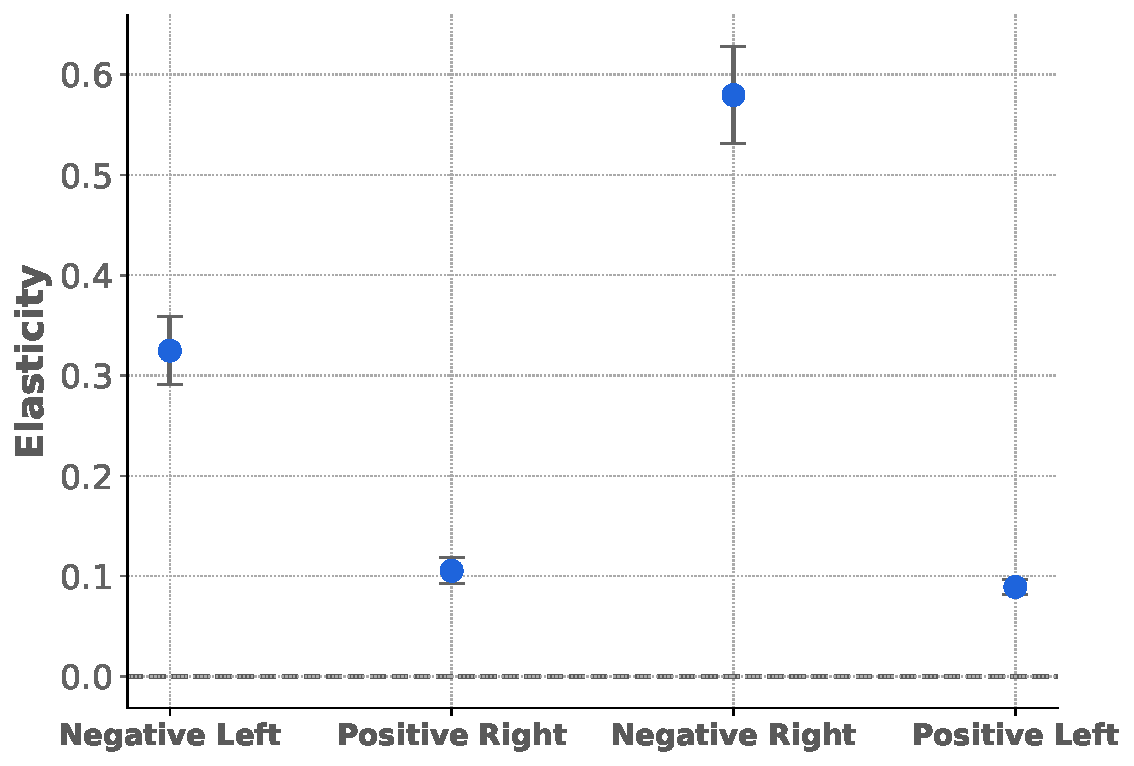
\includegraphics[width=\linewidth]{figures/elasticities_right_pre}
			\label{fig:2figsA}
		\end{minipage}
		
		\vspace{0.5em} % space between figures and note
		
		\captionsetup{justification=justified}
		\caption*{\small \textit{Note:} Each panel shows estimated mean own elasticities for consumer responses  as described in Eq. \eqref{eq:elasticities} for the off-campaign period. Panel (a) reports results for the left-leaning markets, while Panel (b) shows the results for the right-leaning markets. Right markets are defined as regions with proportion of right-wing voters above the median. Whiskers represent the $95\%$ confidence intervals of the mean across markets.}
	\end{figure}
	
	
	
	\begin{figure}[ht!]
		\centering
		\caption{Added Variable Plots for Production of Political Content (within day)}
		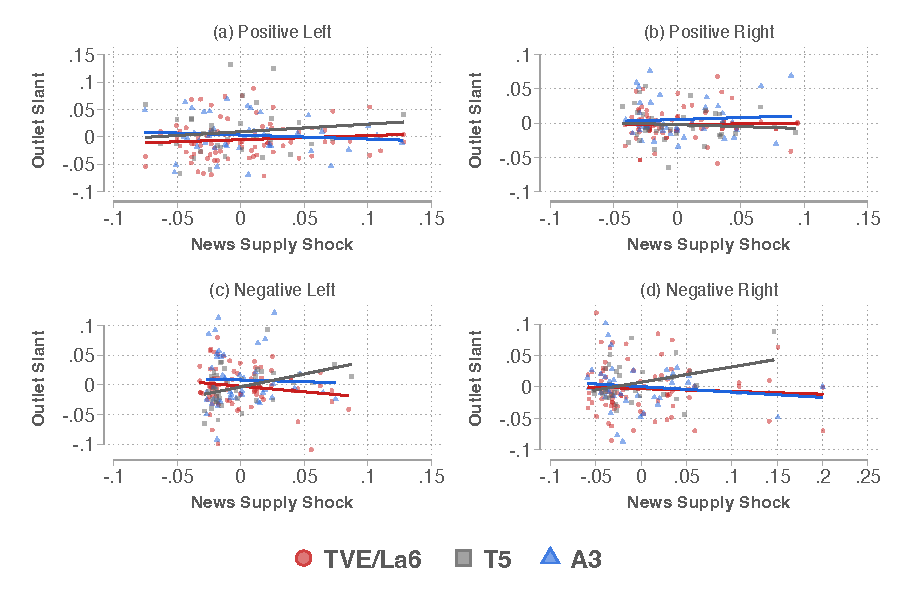
\includegraphics[width=160mm]{figures/fwl_plots_lowess_diff_costs_v2}
		\caption*{\small \textit{Note:} The figure shows the added variable plots from the analogous estimation of Eq. \eqref{eq:first_stage} using within day differences. The x axis represents $\left(\Delta z_d^{party,+},\Delta z_d^{party,-}\right) $ and the y axis the corresponding  $\left(\Delta x_{jd}^{party,+},\Delta x_{jd}^{party,-}\right) $   . Channels are pooled into left (TVE and La Sexta), middle (T5) and right (A3) for visualization purposes.  }
		\label{fig:fwl_diff}
	\end{figure}
	
	
	
	\begin{figure}[!htb]
		\caption{Within-day Relationship Between Editorial Content Share and News Supply Shock}
		\centering
		\begin{tabular}{@{}cc@{}}
			% Panel headers row
			\text{(a) Positive Left } &
			\text{(b) Positive Right} \\[0.08em]
			% First row of plots
			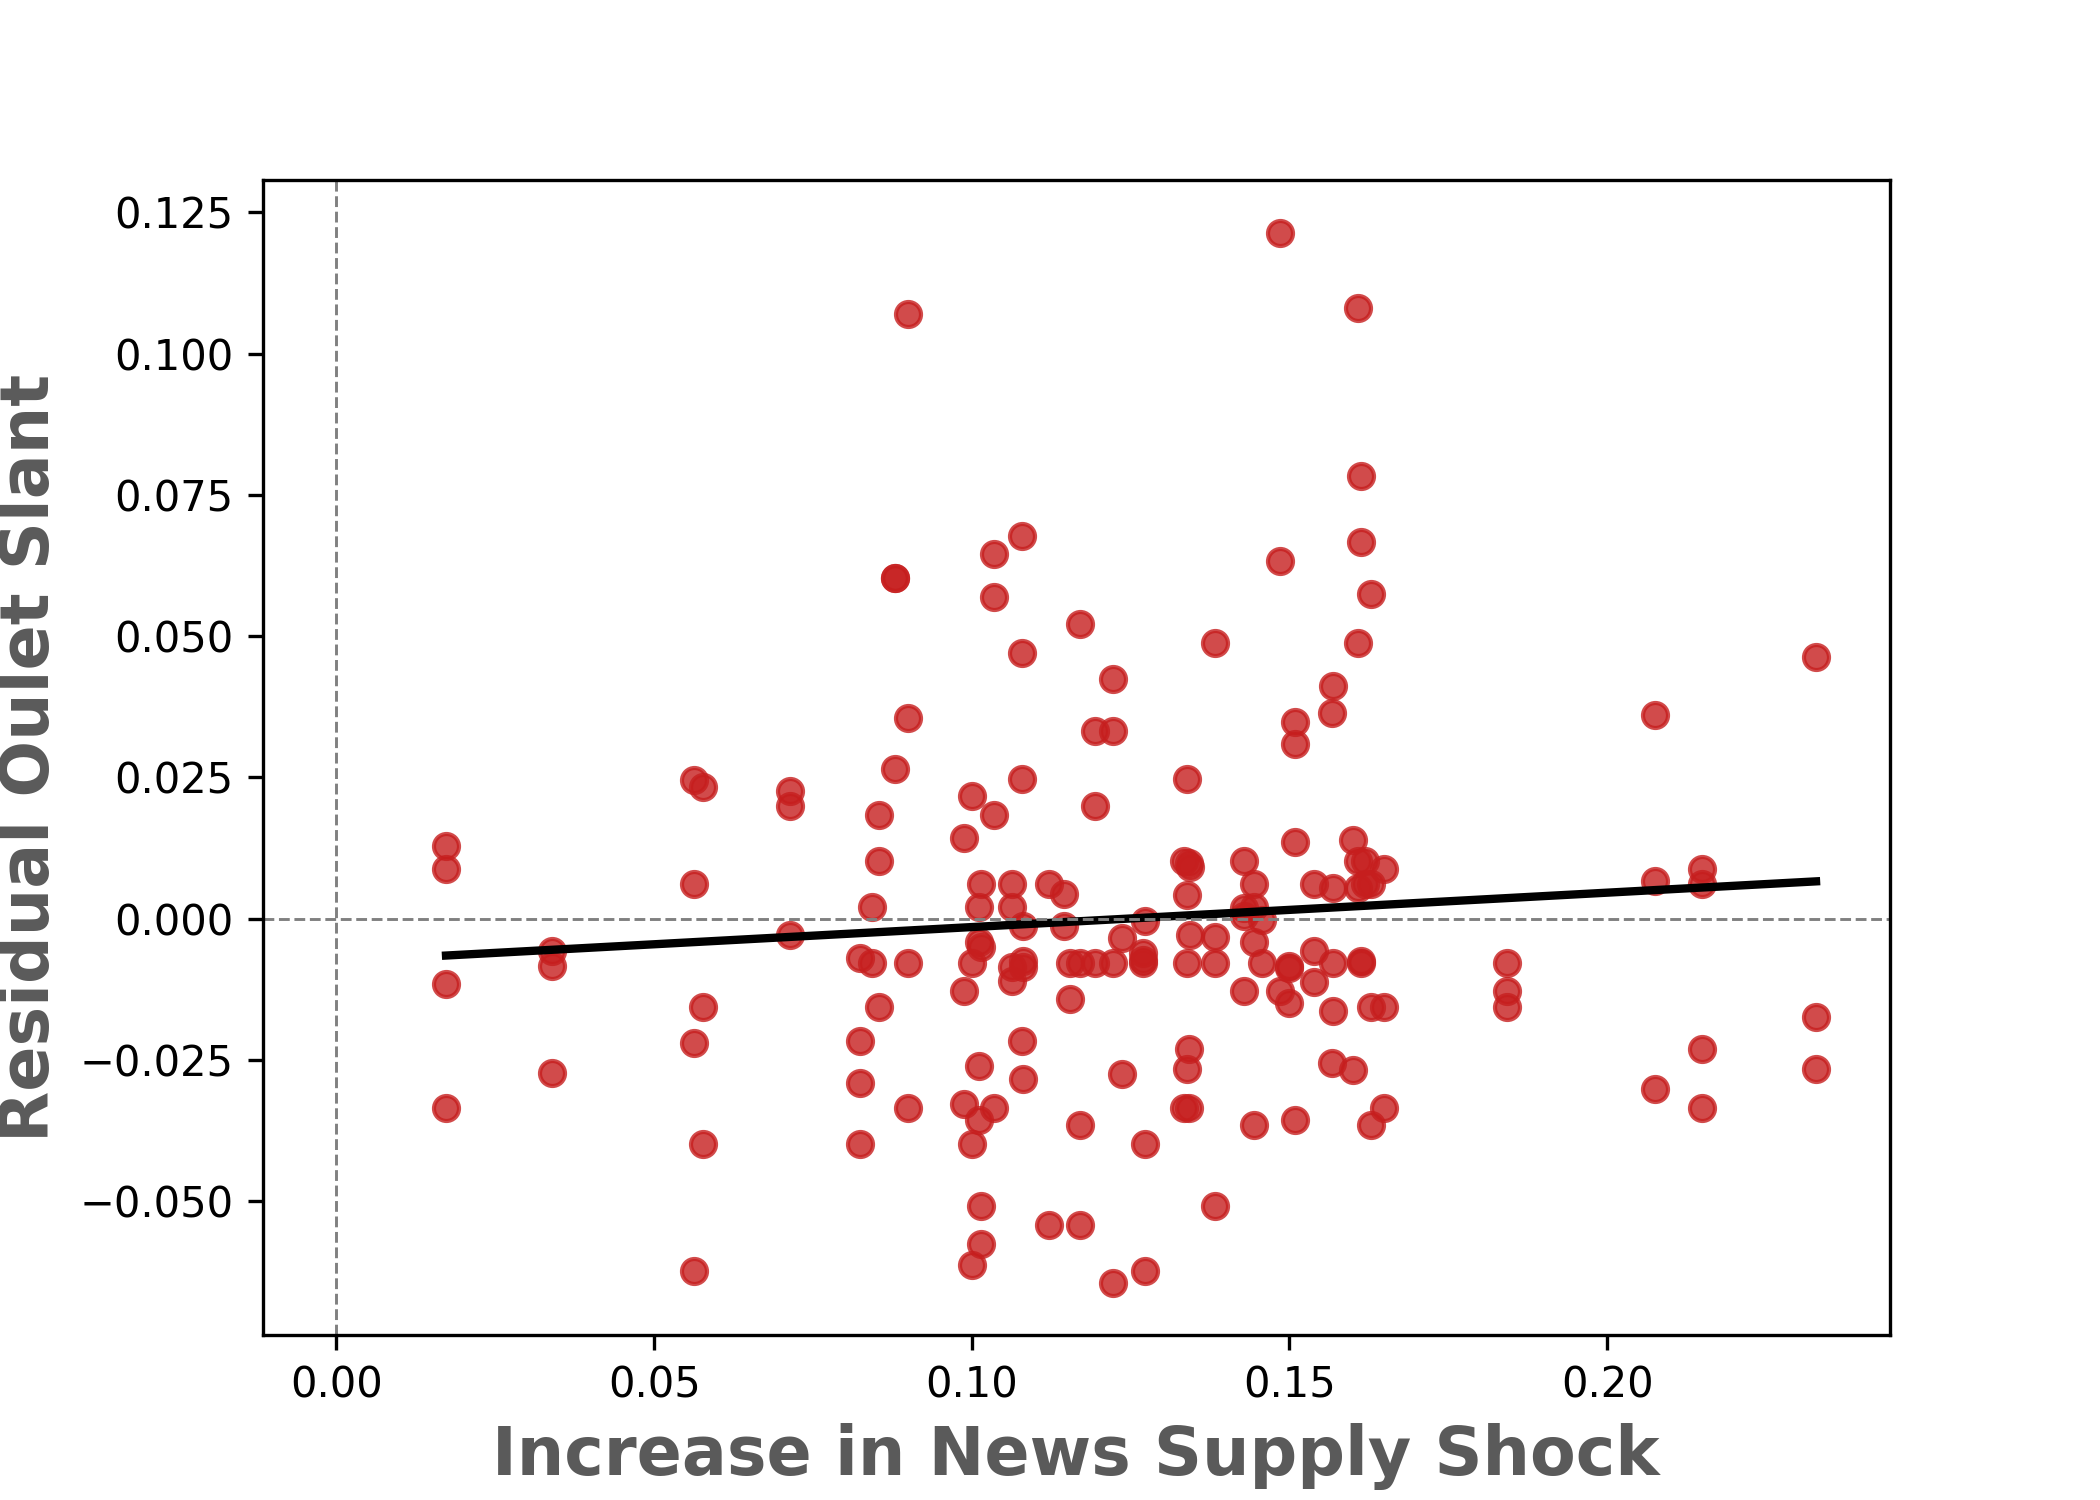
\includegraphics[width=0.45\textwidth]{figures/char_pos_left_residual_v2} &
			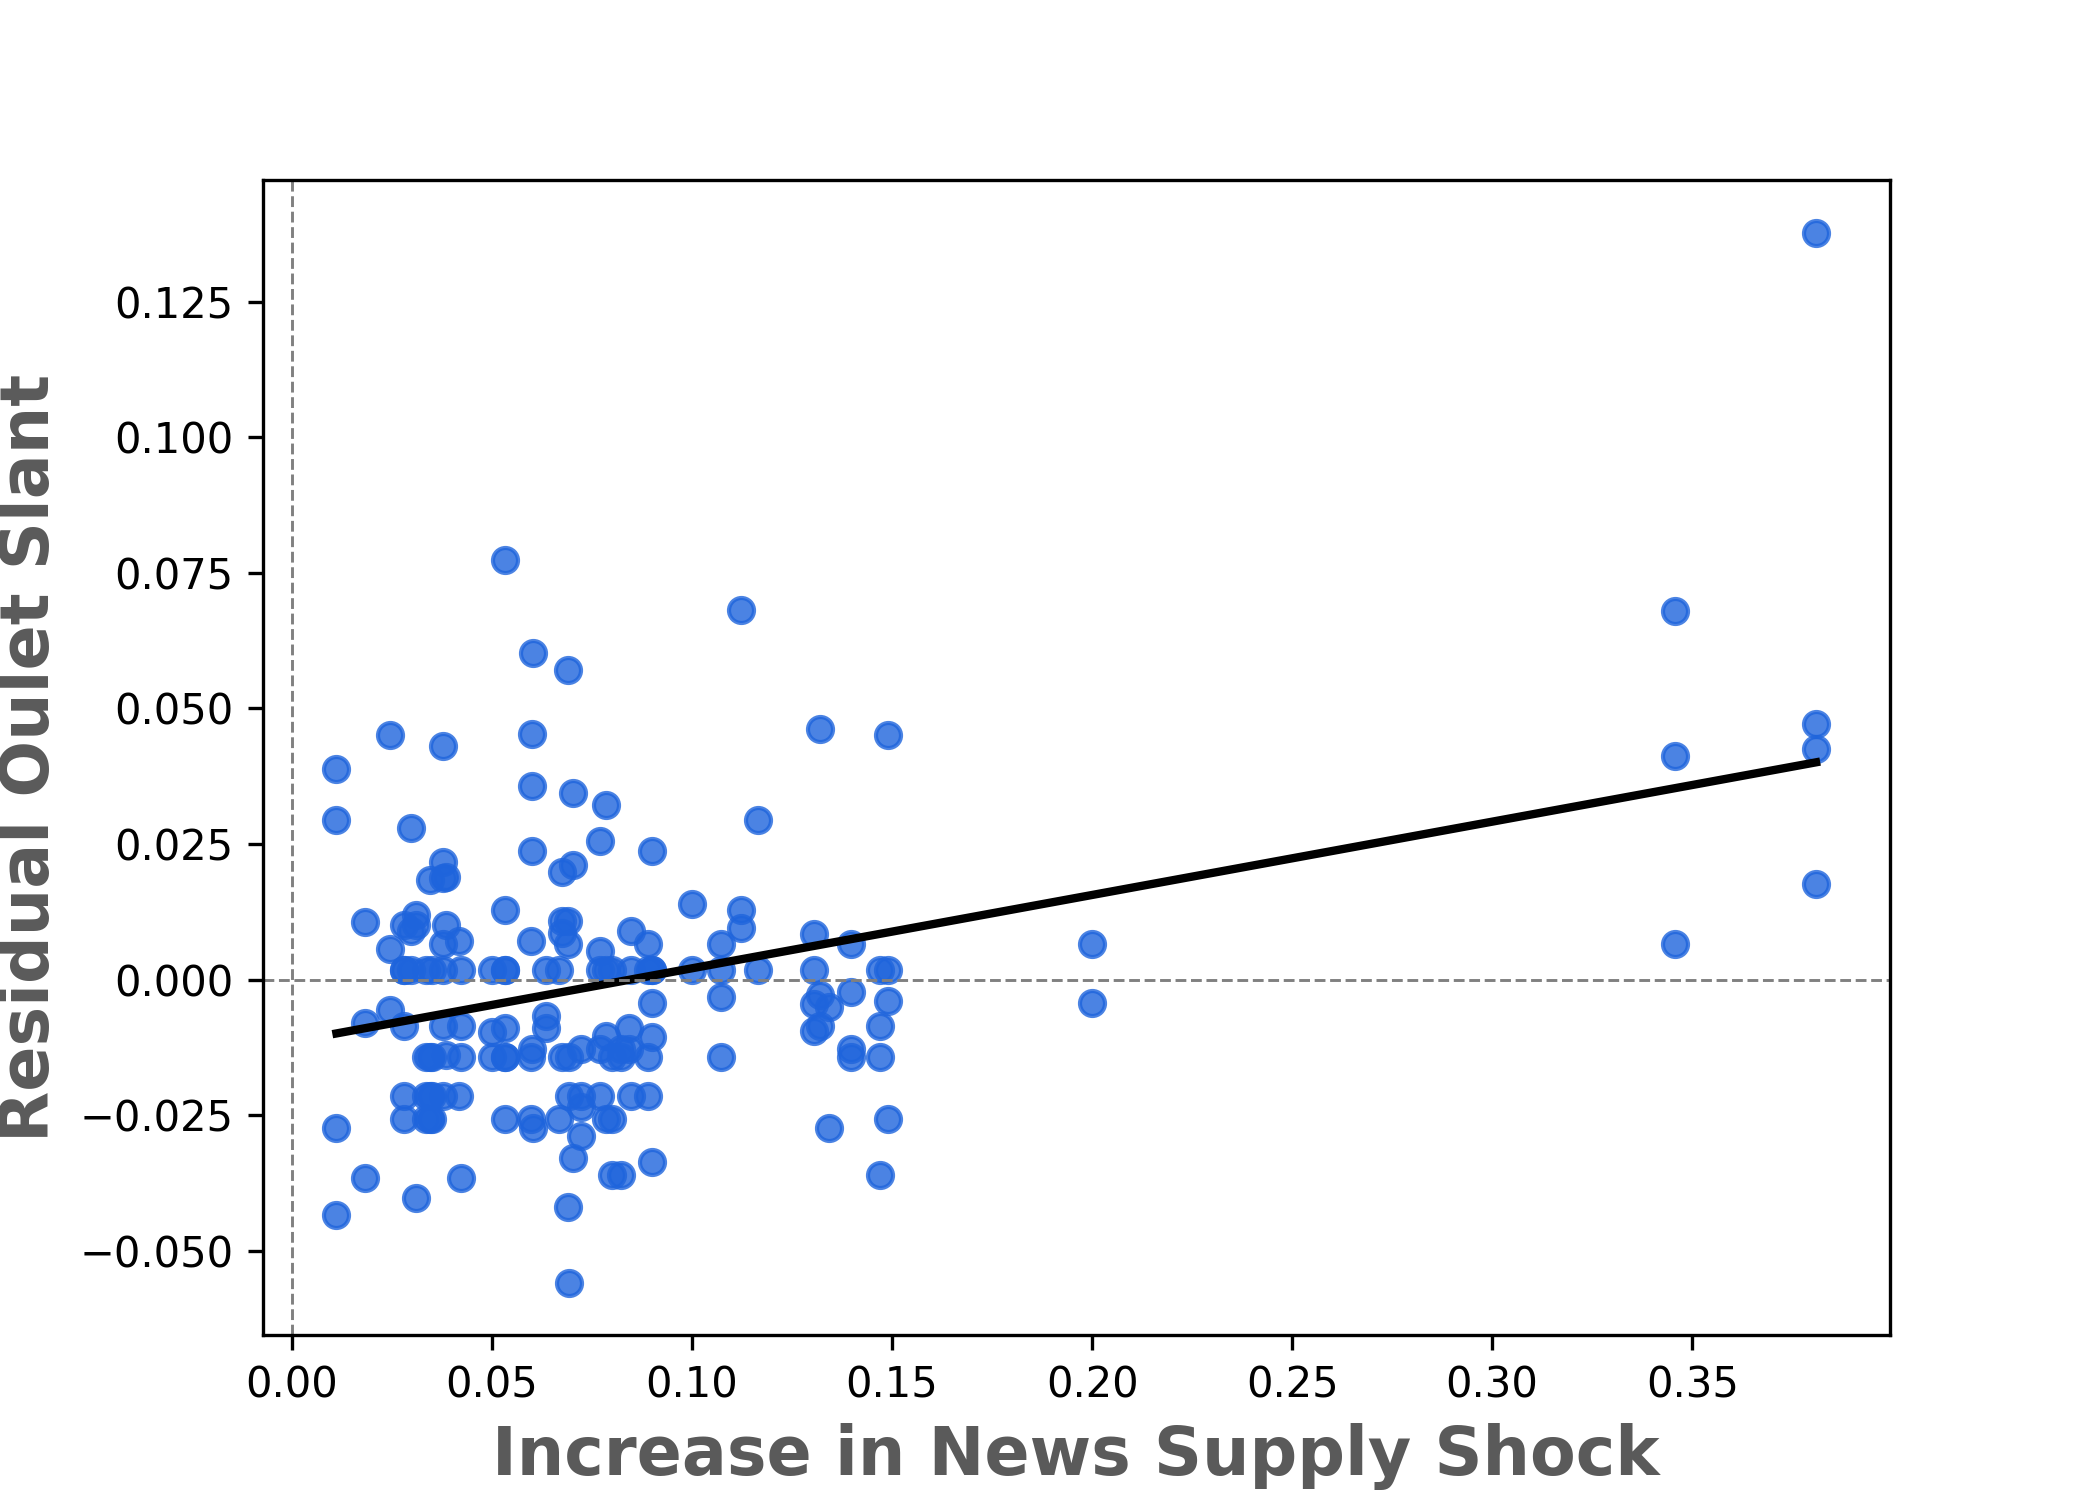
\includegraphics[width=0.45\textwidth]{figures/char_pos_right_residual_v2} \\[1em]
			% Panel headers row
			\text{(c) Negative Left} &
			\text{(d) Negative Right} \\[0.08em]
			% Second row of plots
			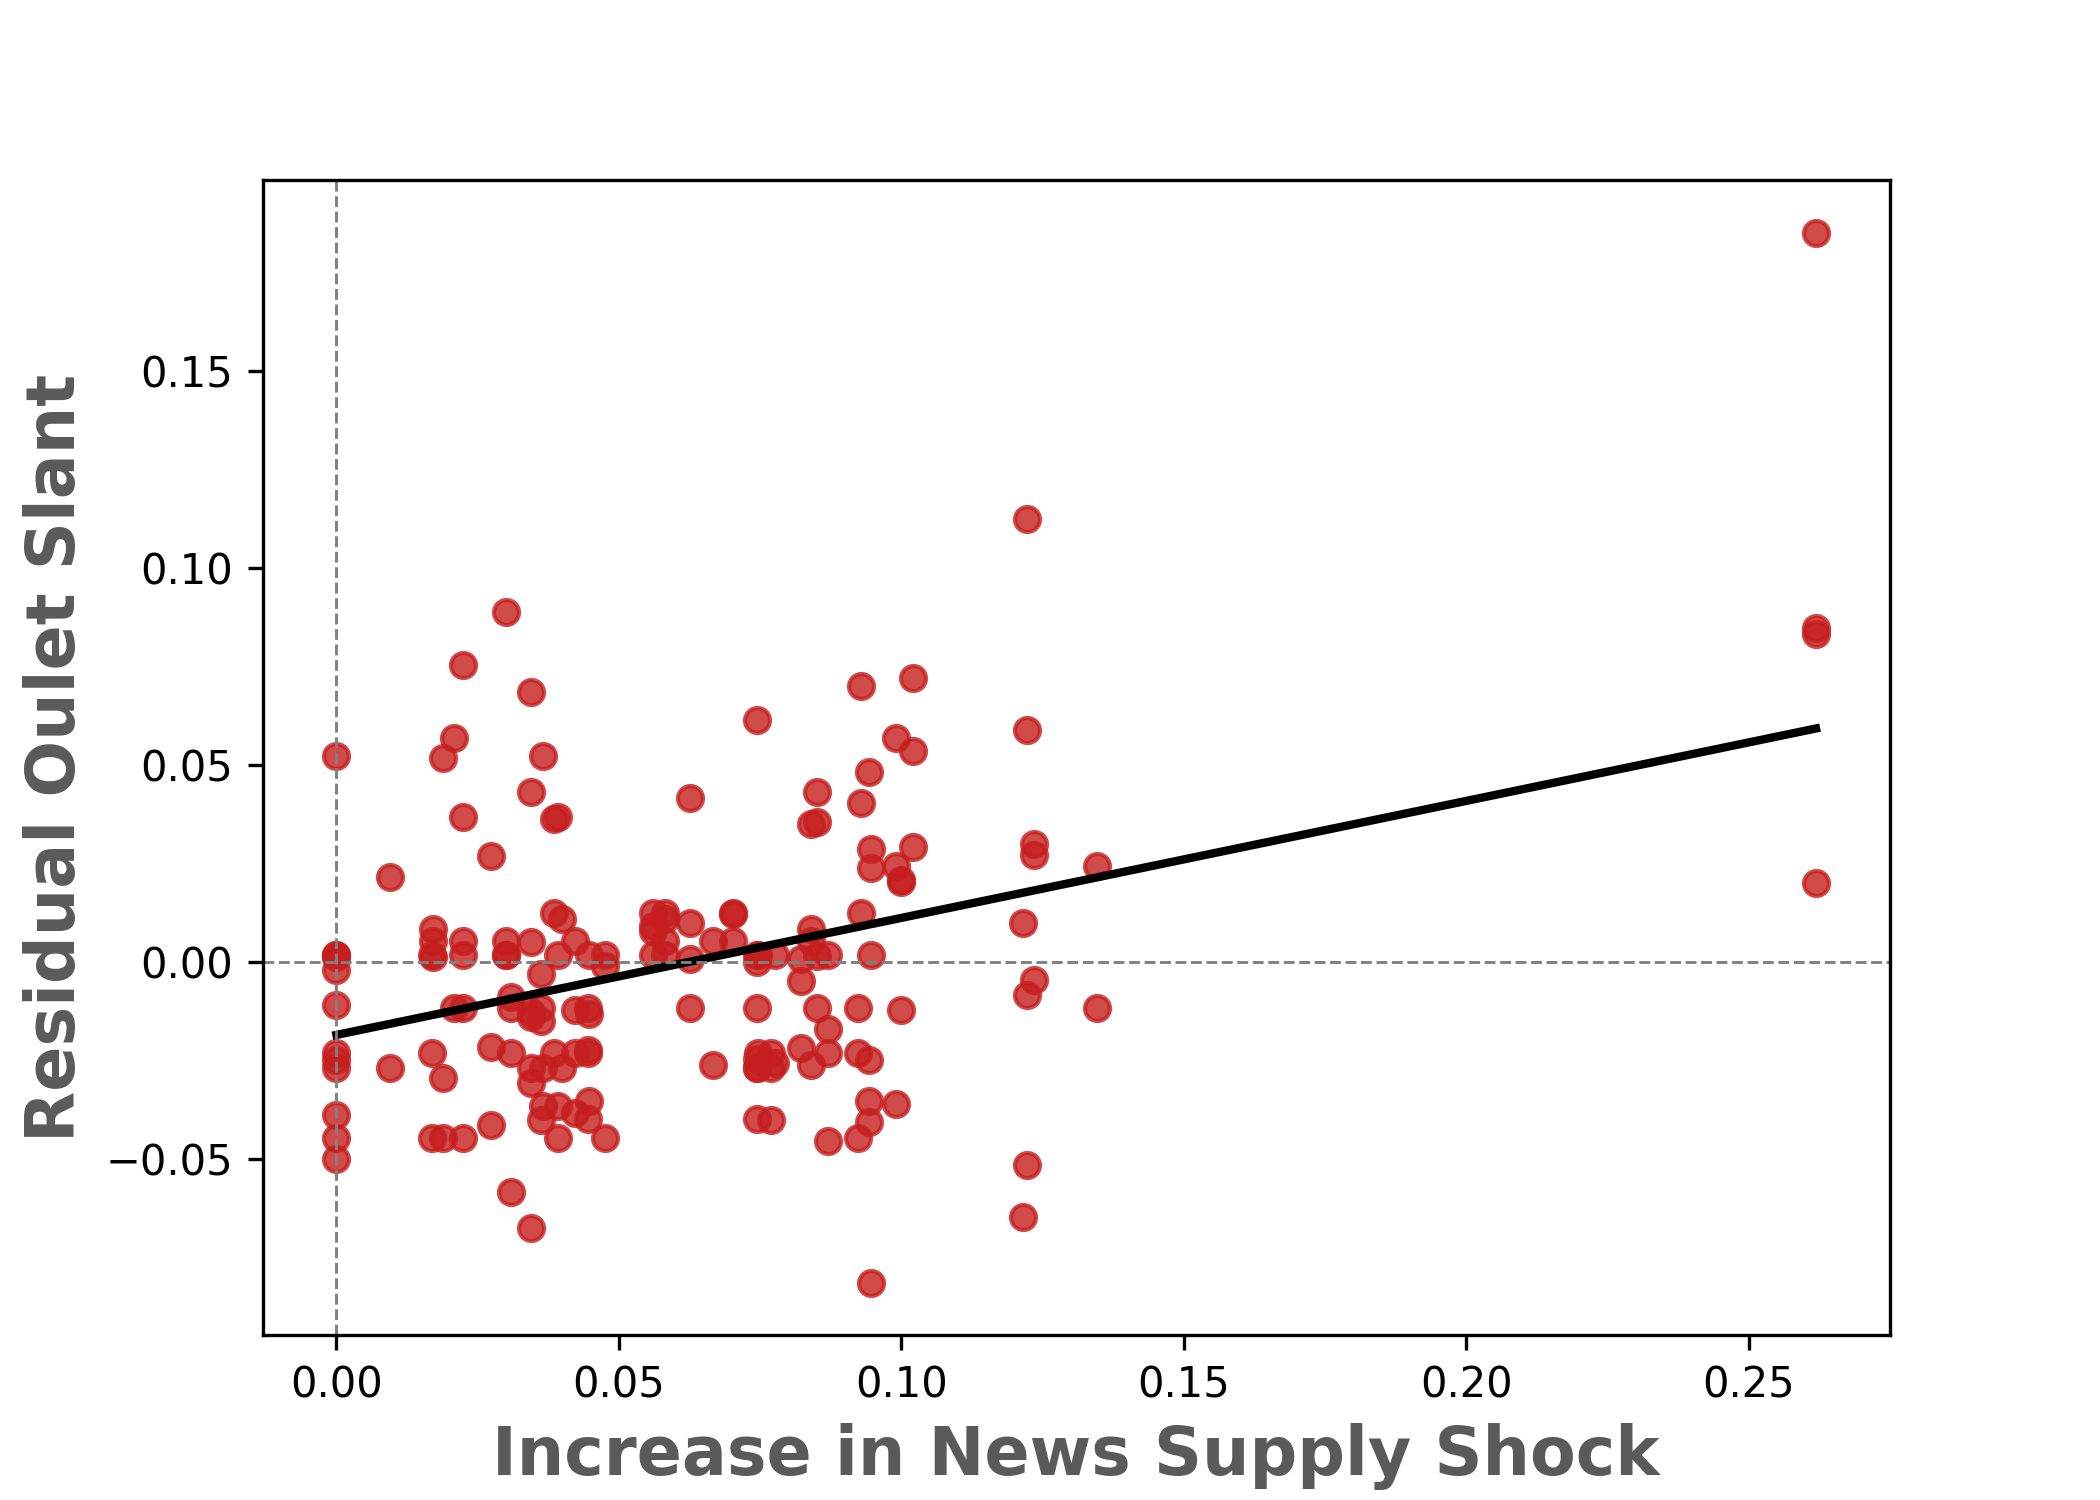
\includegraphics[width=0.45\textwidth]{figures/char_neg_left_residual_v2} &
			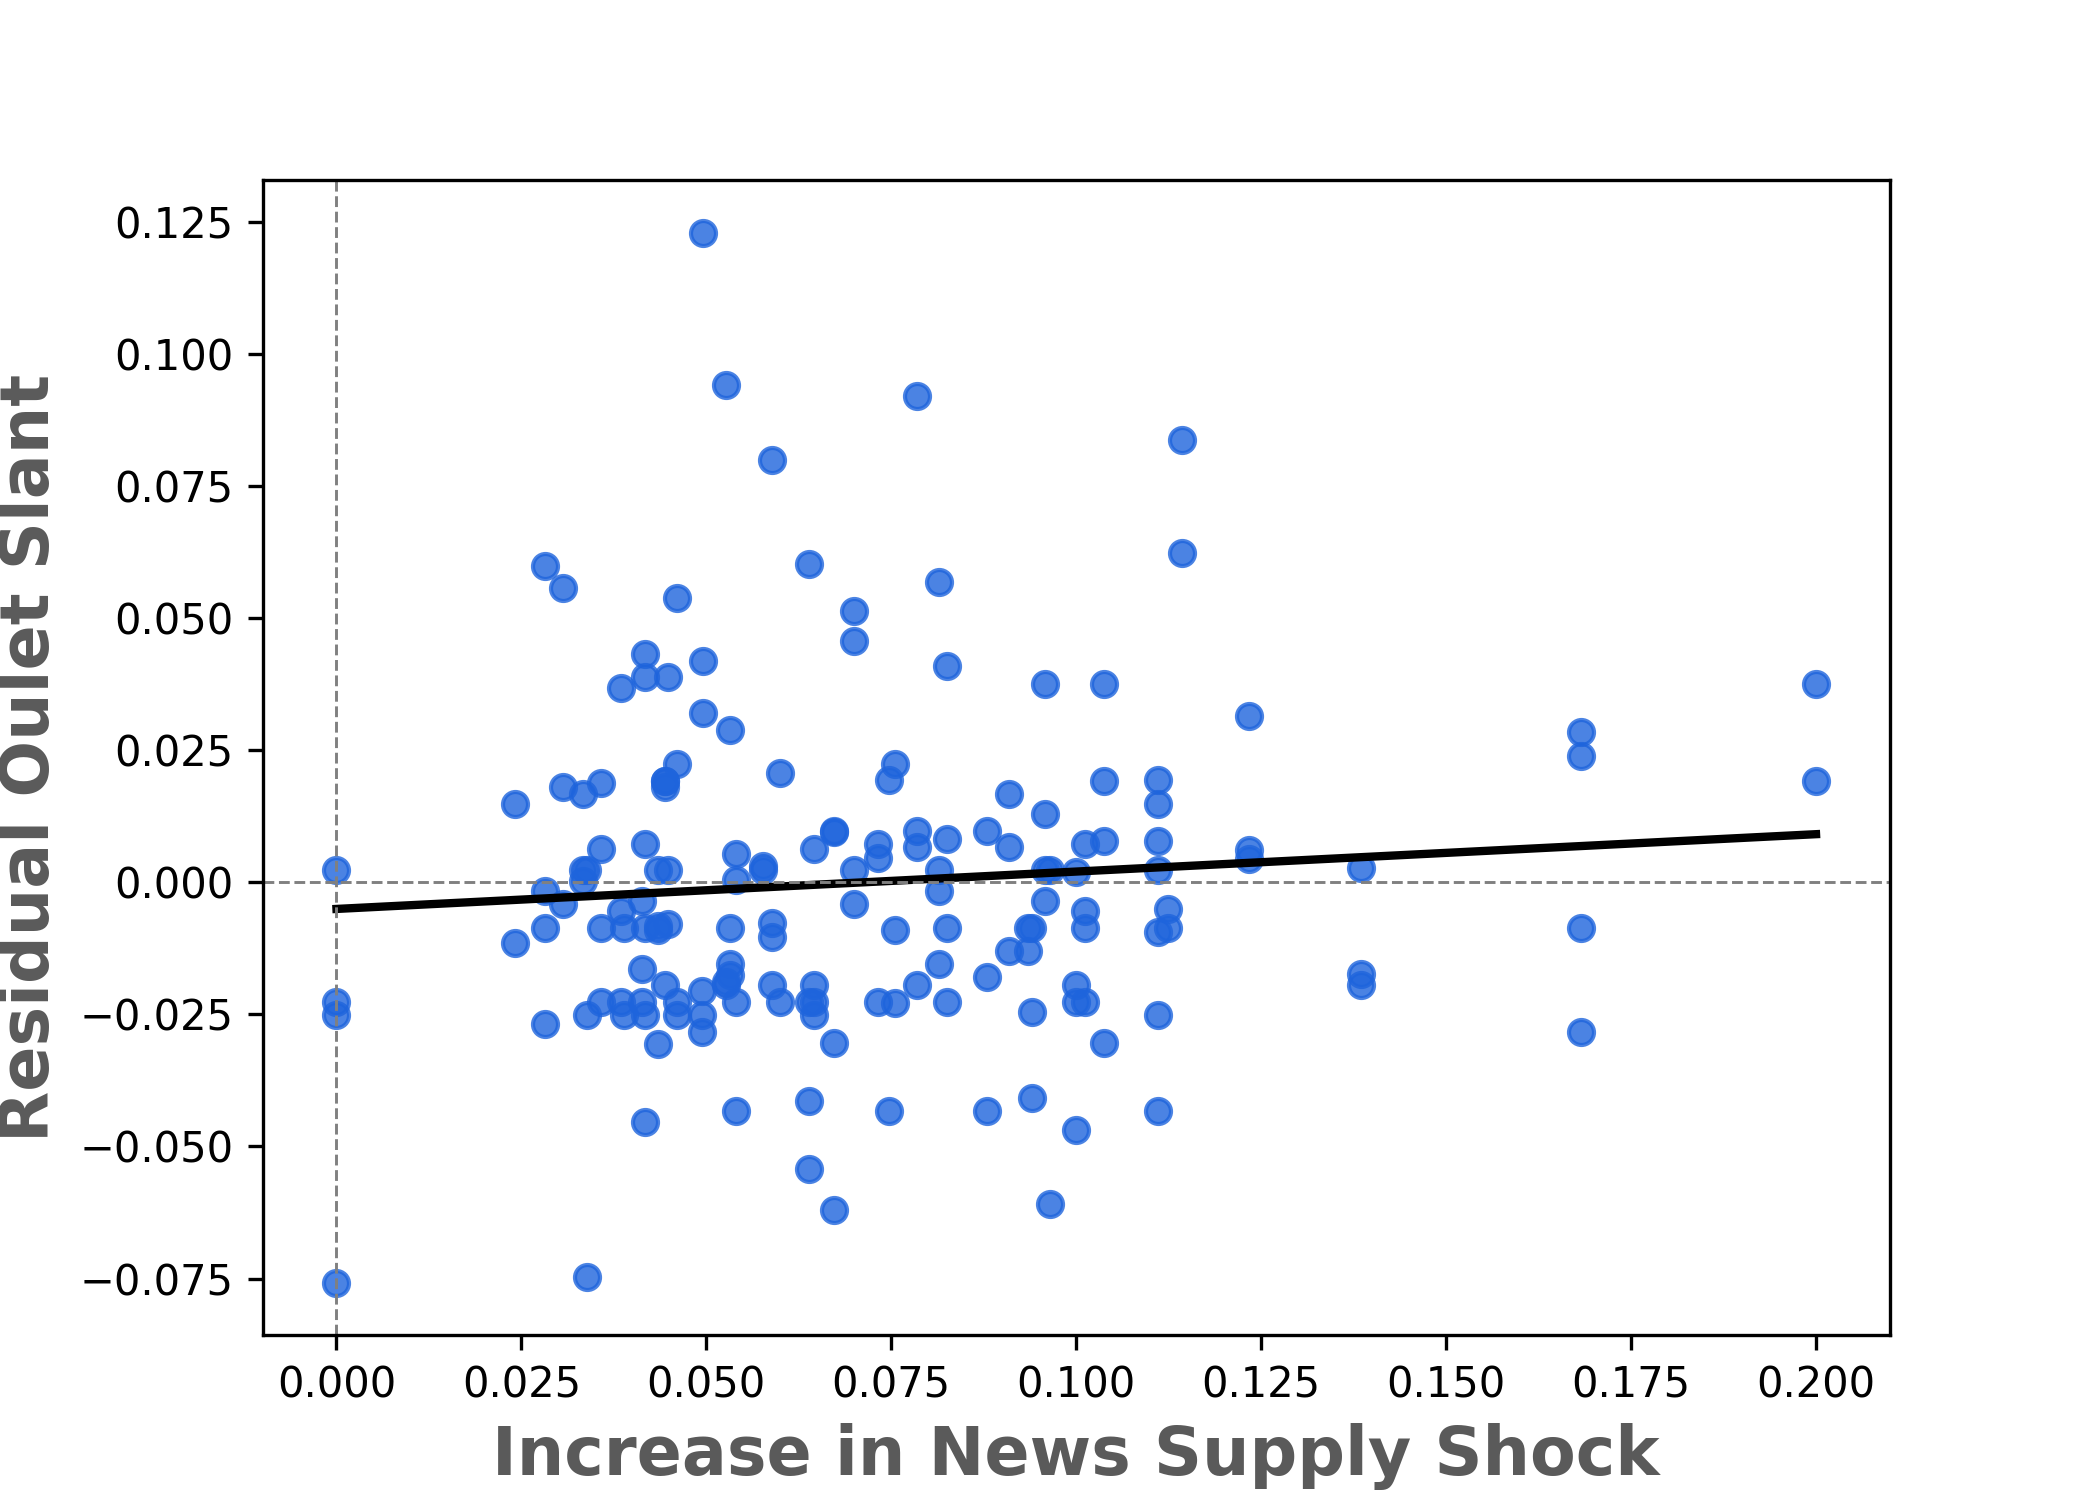
\includegraphics[width=0.45\textwidth]{figures/char_neg_right_residual_v2}
		\end{tabular}
		\caption*{\small \textit{Note:} Scatterplots of the within-day relationship between channels' editorial content share ($x$) 
			and the corresponding news supply shock ($z$) from Agencia EFE. Each panel corresponds to one type of coverage: 
			(a) positive-left, (b) positive-right, (c) negative-left, and (d) negative-right. The $y$-axis plots the residuals from 
			a regression of evening content share on midday content share with outlet fixed effects, capturing variation in evening 
			coverage not explained by earlier coverage. The $x$-axis shows the share of EFE stories of the corresponding type published 
			between midday and evening. Lines represent fitted values from ordinary least squares. }
		\label{fig:diff}
	\end{figure}
	
	
	
		\begin{figure}[!htb]
		\caption{Outlet's Payoffs for each Tone Category}
		\centering
		\begin{tabular}{@{}cc@{}}
			% Panel headers row
			\text{(a) Positive Left } &
			\text{(b) Positive Right} \\[0.08em]
			% First row of plots
			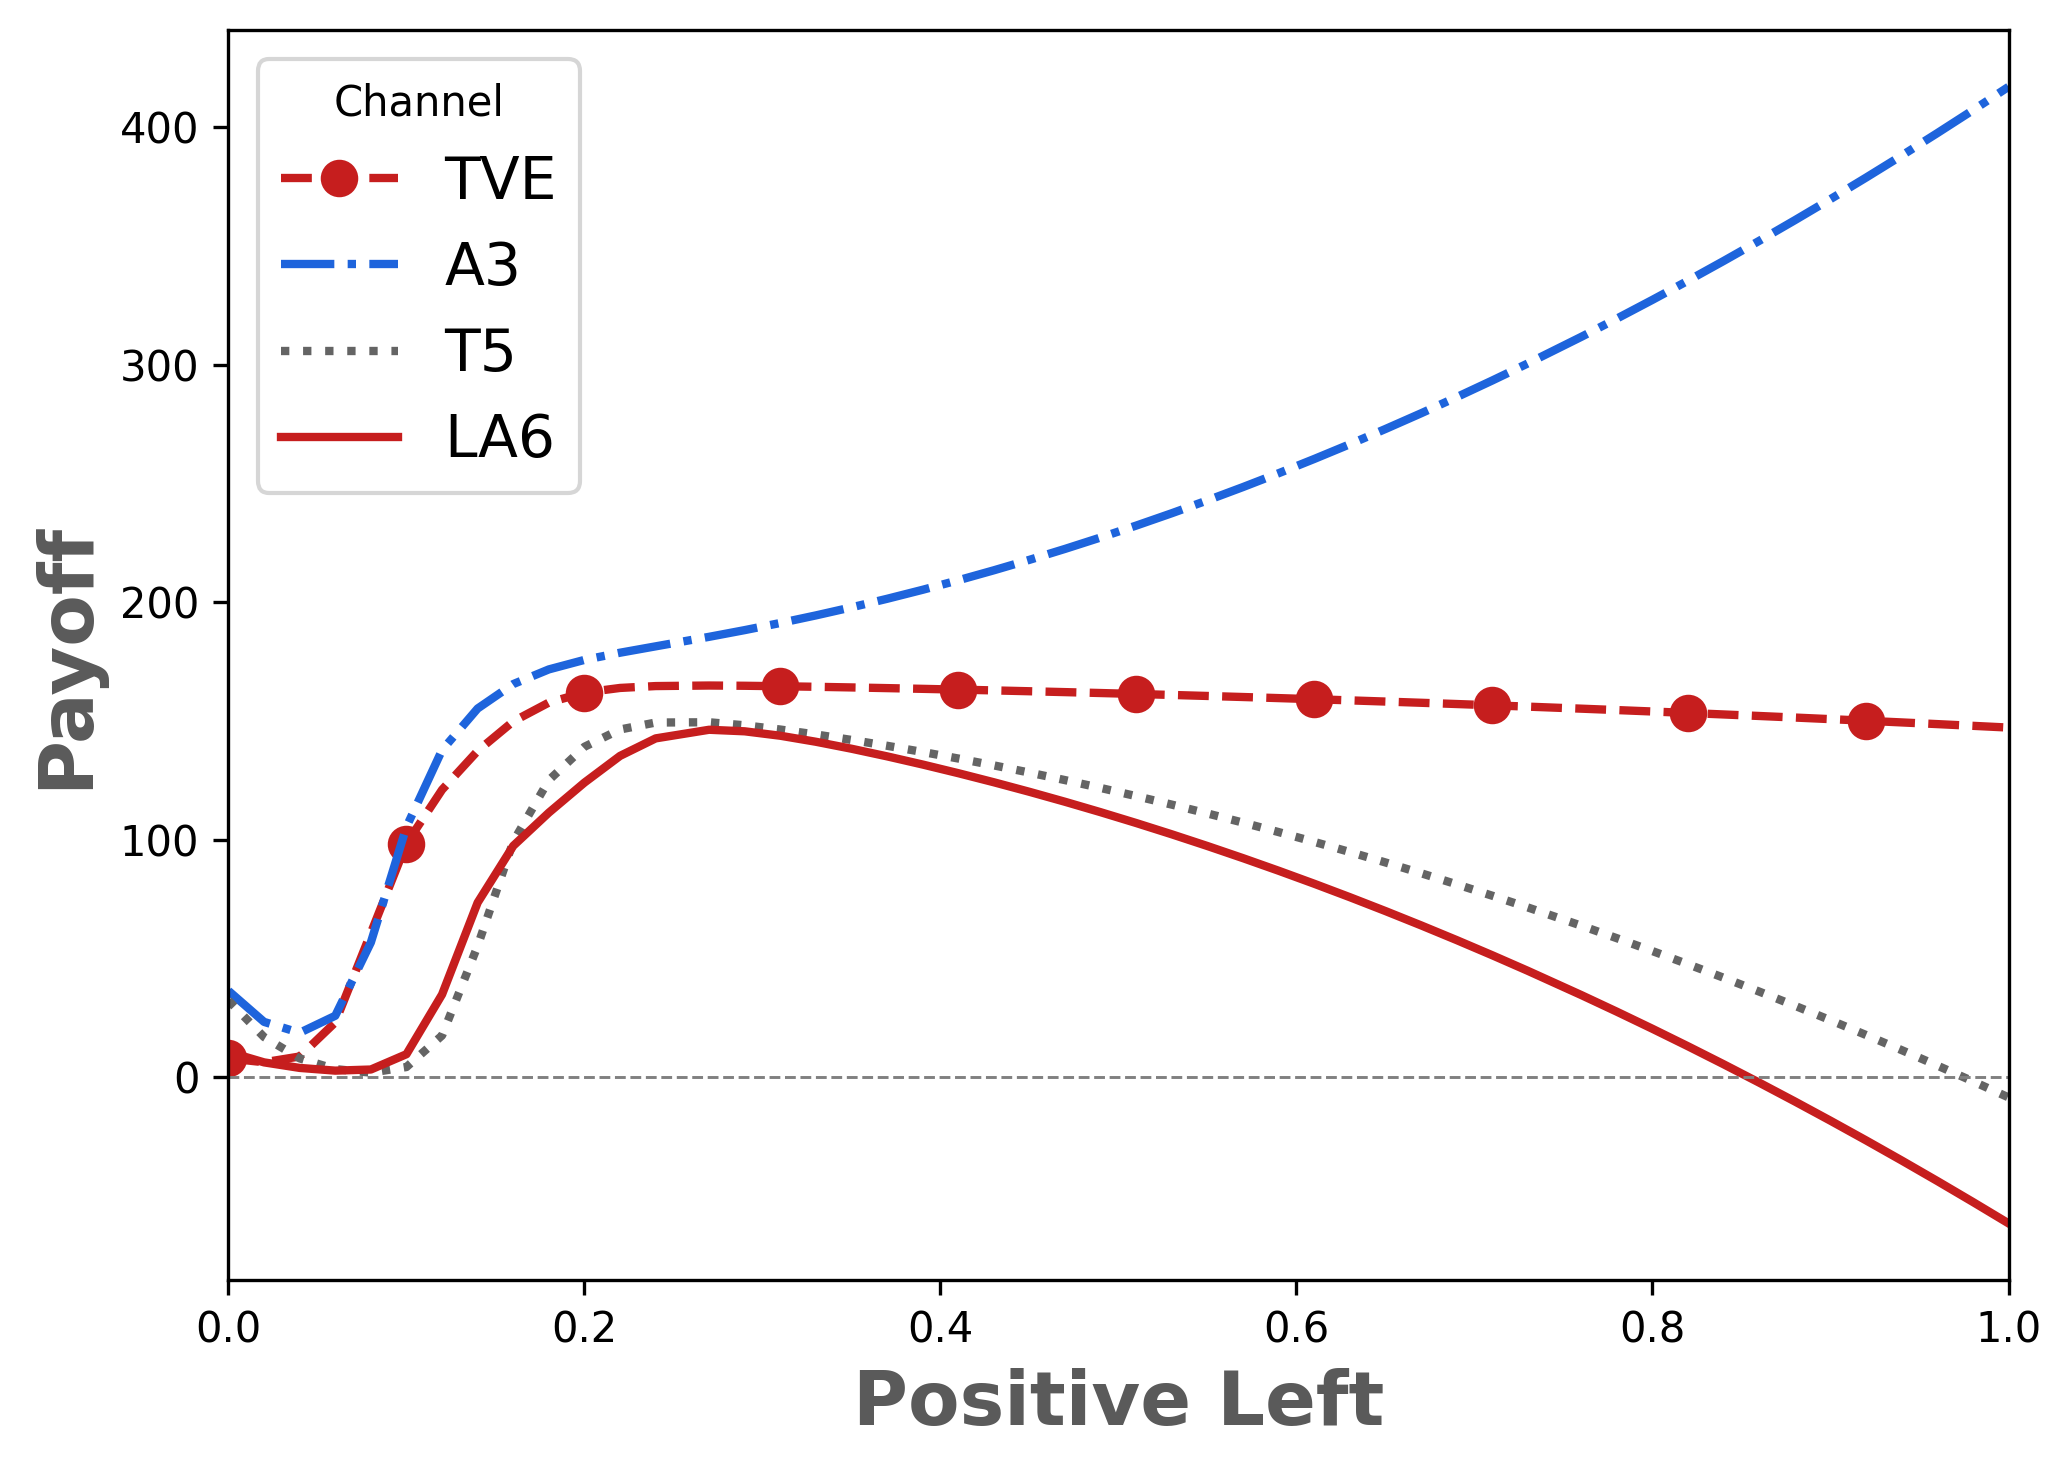
\includegraphics[width=0.45\textwidth]{figures/payoff_pos_left} &
			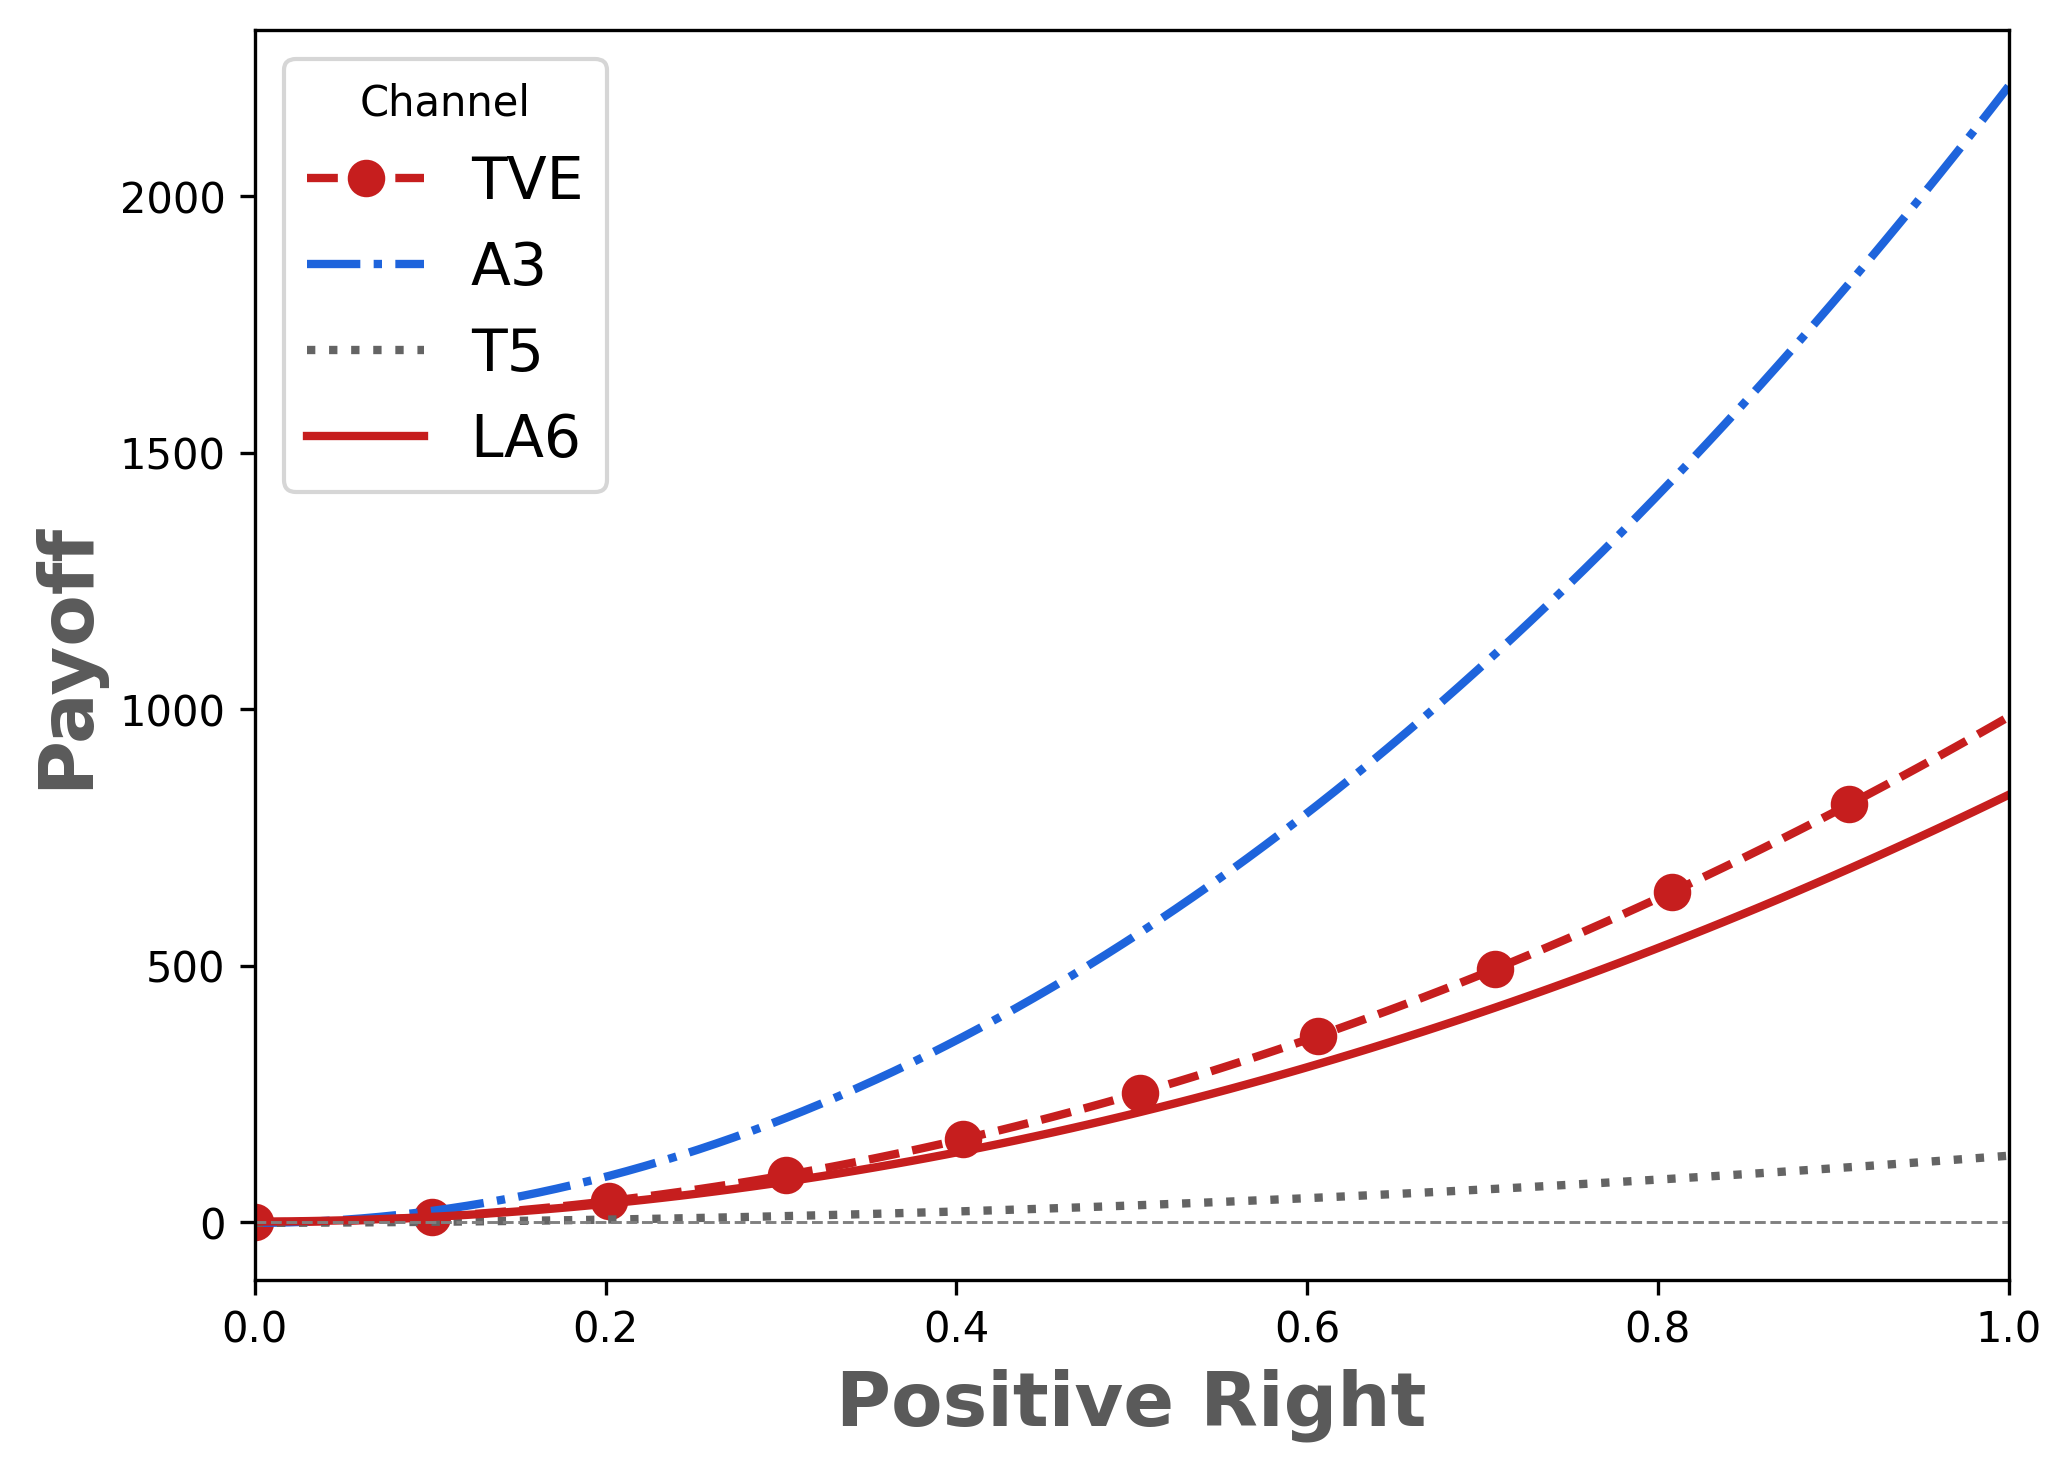
\includegraphics[width=0.45\textwidth]{figures/payoff_pos_right} \\[1em]
			% Panel headers row
			\text{(c) Negative Left} &
			\text{(d) Negative Right} \\[0.08em]
			% Second row of plots
			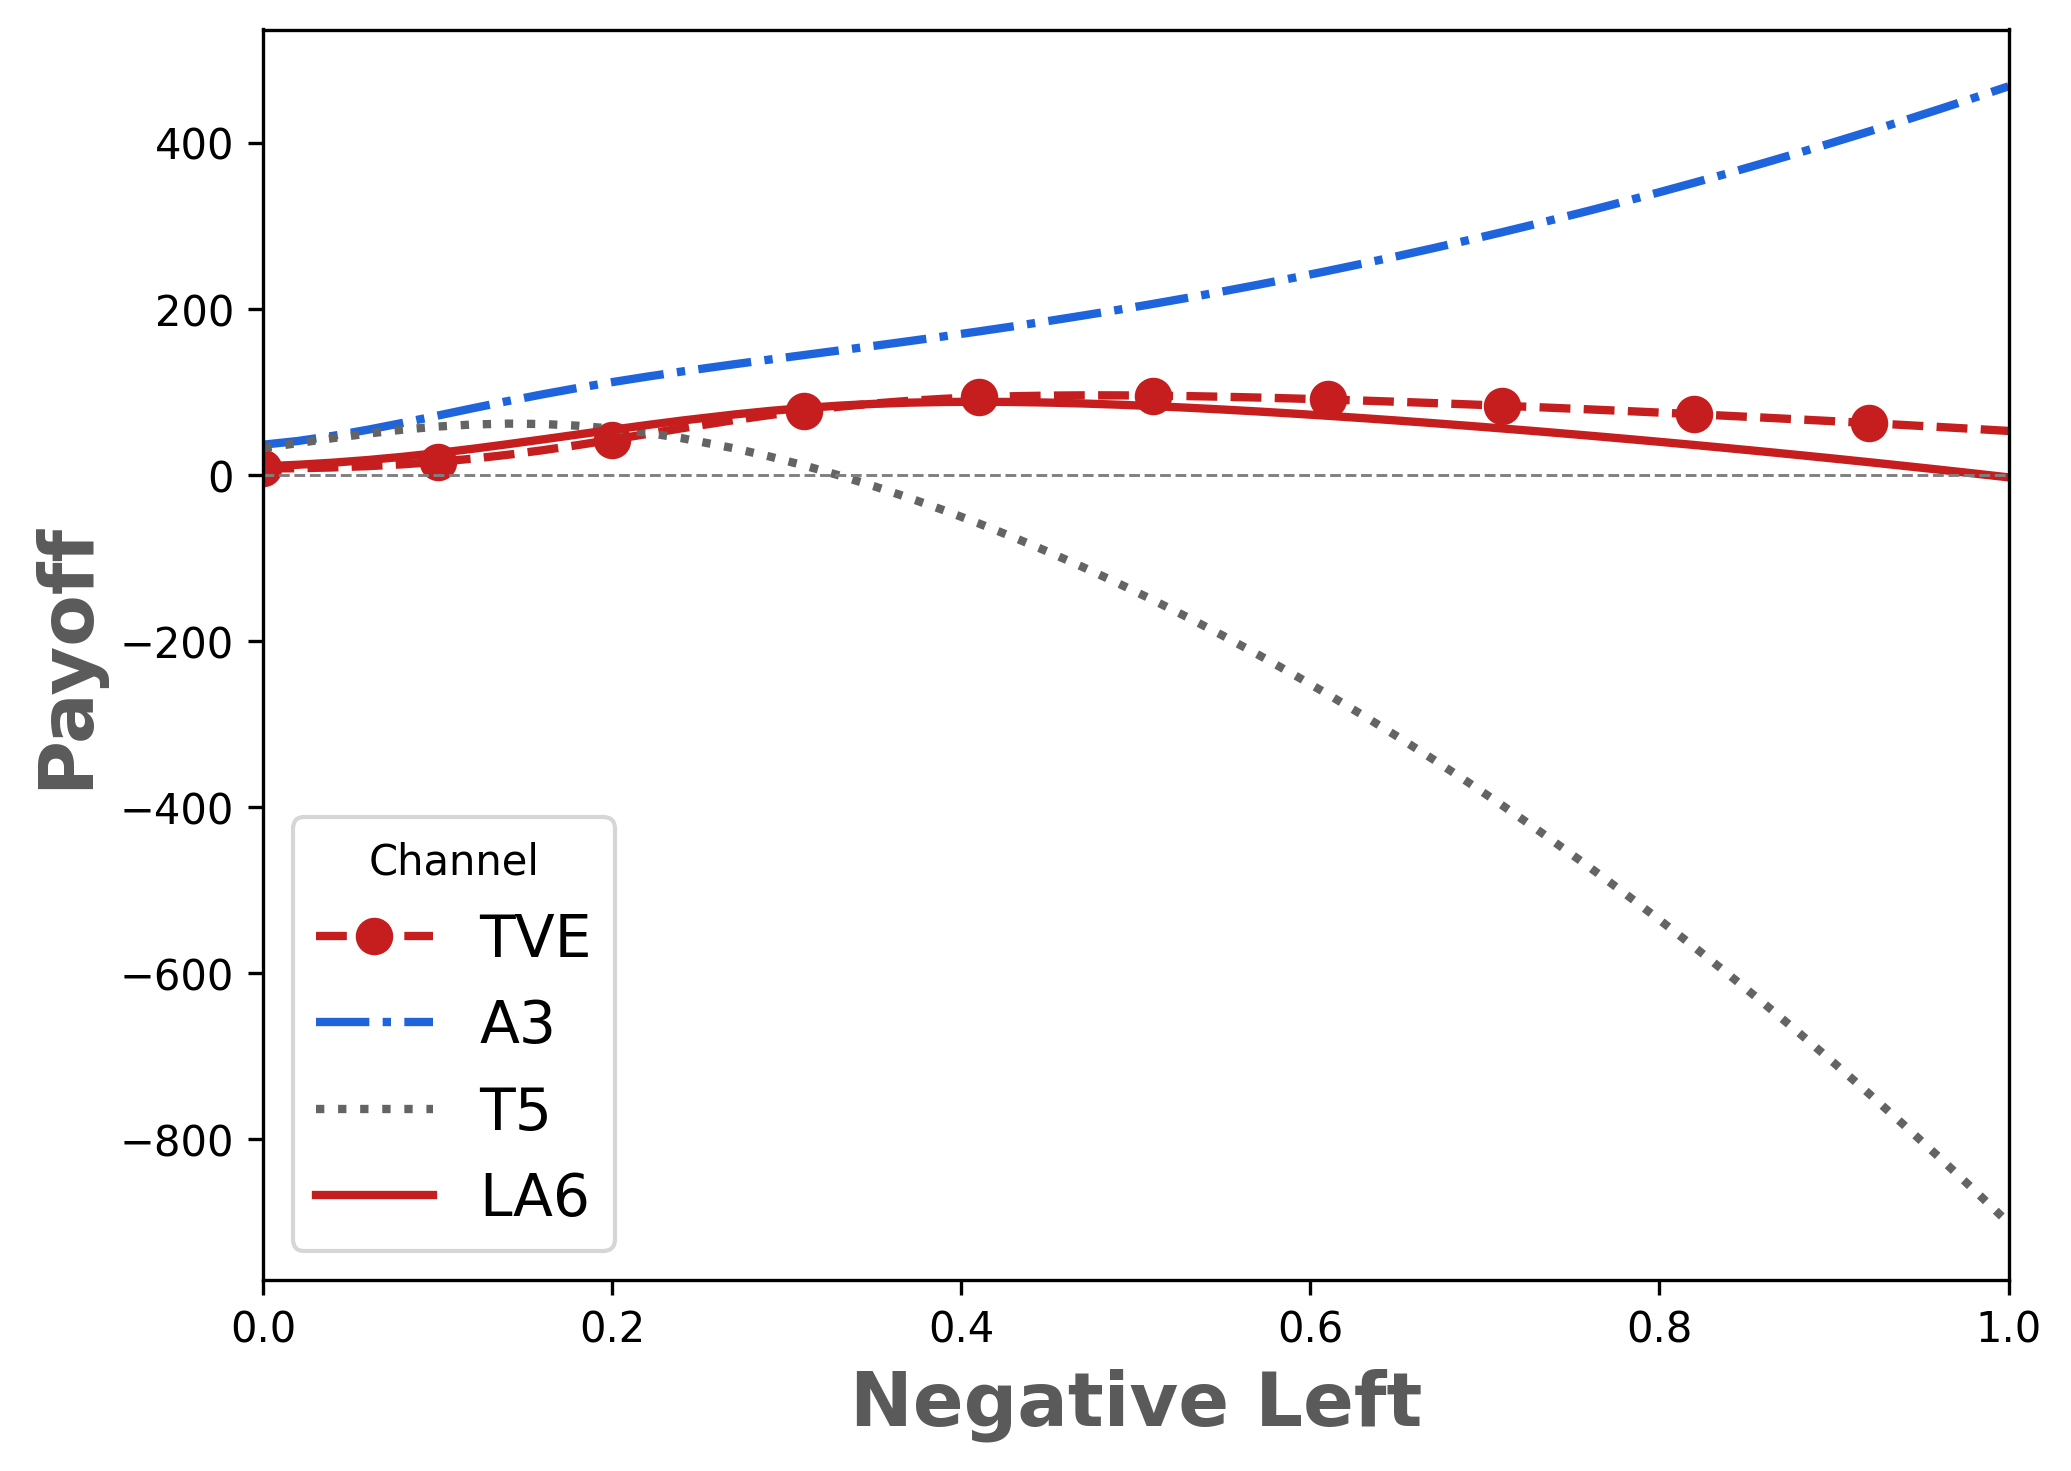
\includegraphics[width=0.45\textwidth]{figures/payoff_neg_left} &
			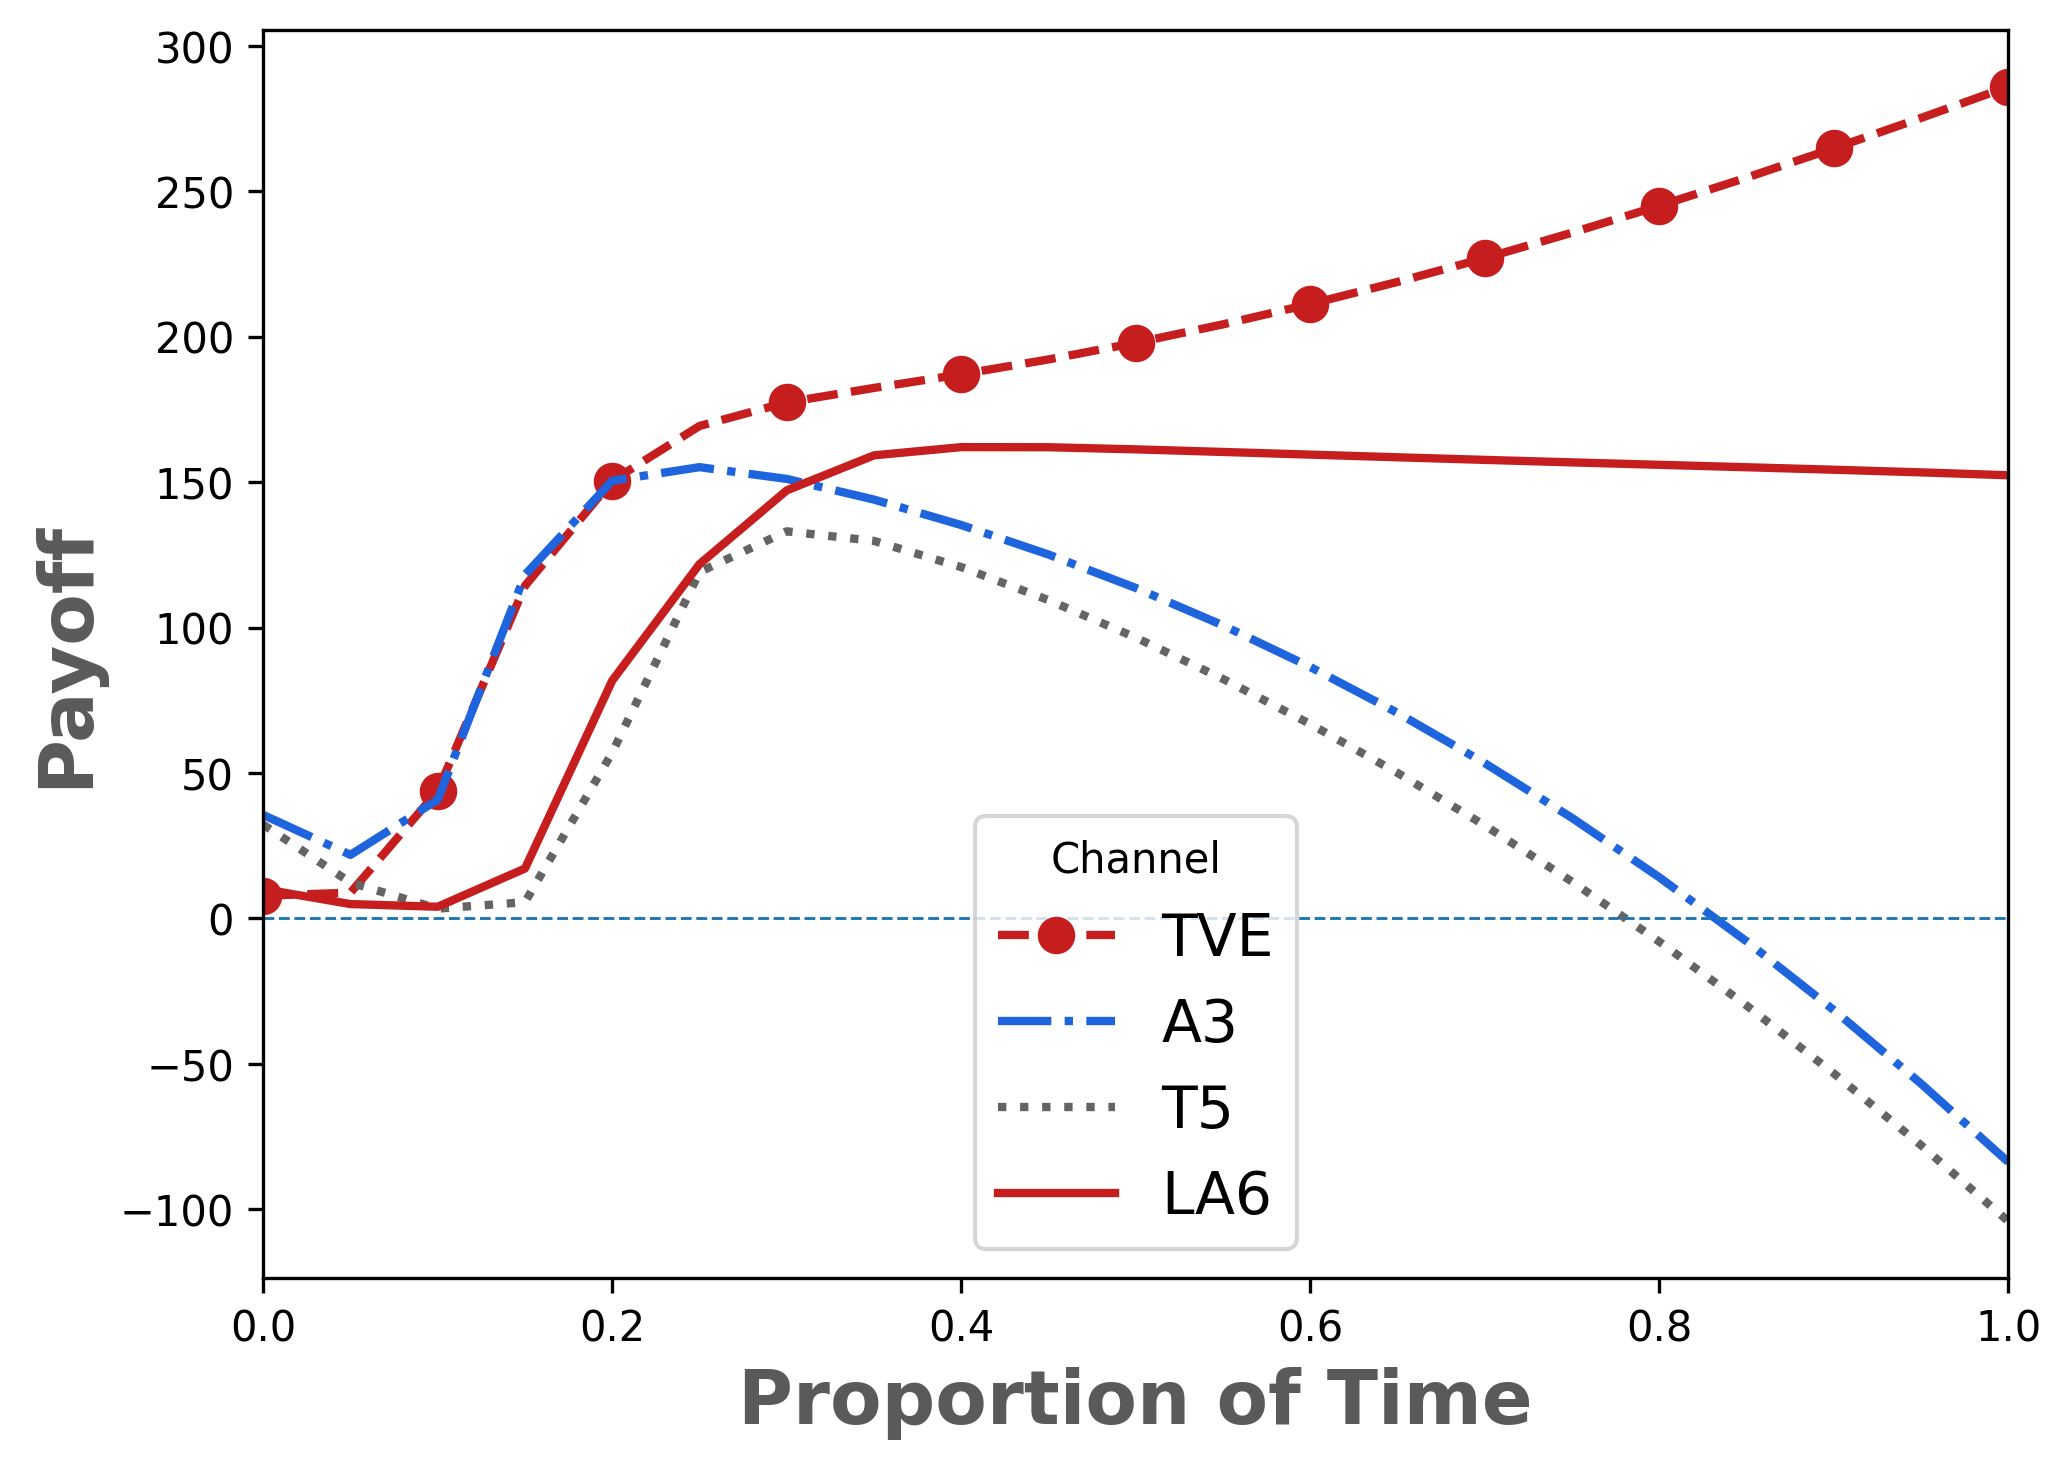
\includegraphics[width=0.45\textwidth]{figures/payoff_neg_right}
		\end{tabular}
		\caption*{\small \textit{Note:} Figures shows the average payoffs of the supply game after estimation. y-axis values represent thousands of viewers. Average are taken over days. Each panel corresponds to one type of coverage: 
			(a) positive-left, (b) positive-right, (c) negative-left, and (d) negative-right.}
		\label{fig:payoffs}
	\end{figure}
	
	
	
		\begin{figure}[!htb]
		\caption{Outlet's Payoffs for each Tone Category (Constrained)}
		\centering
		\begin{tabular}{@{}cc@{}}
			% Panel headers row
			\text{(a) Positive Left } &
			\text{(b) Positive Right} \\[0.08em]
			% First row of plots
			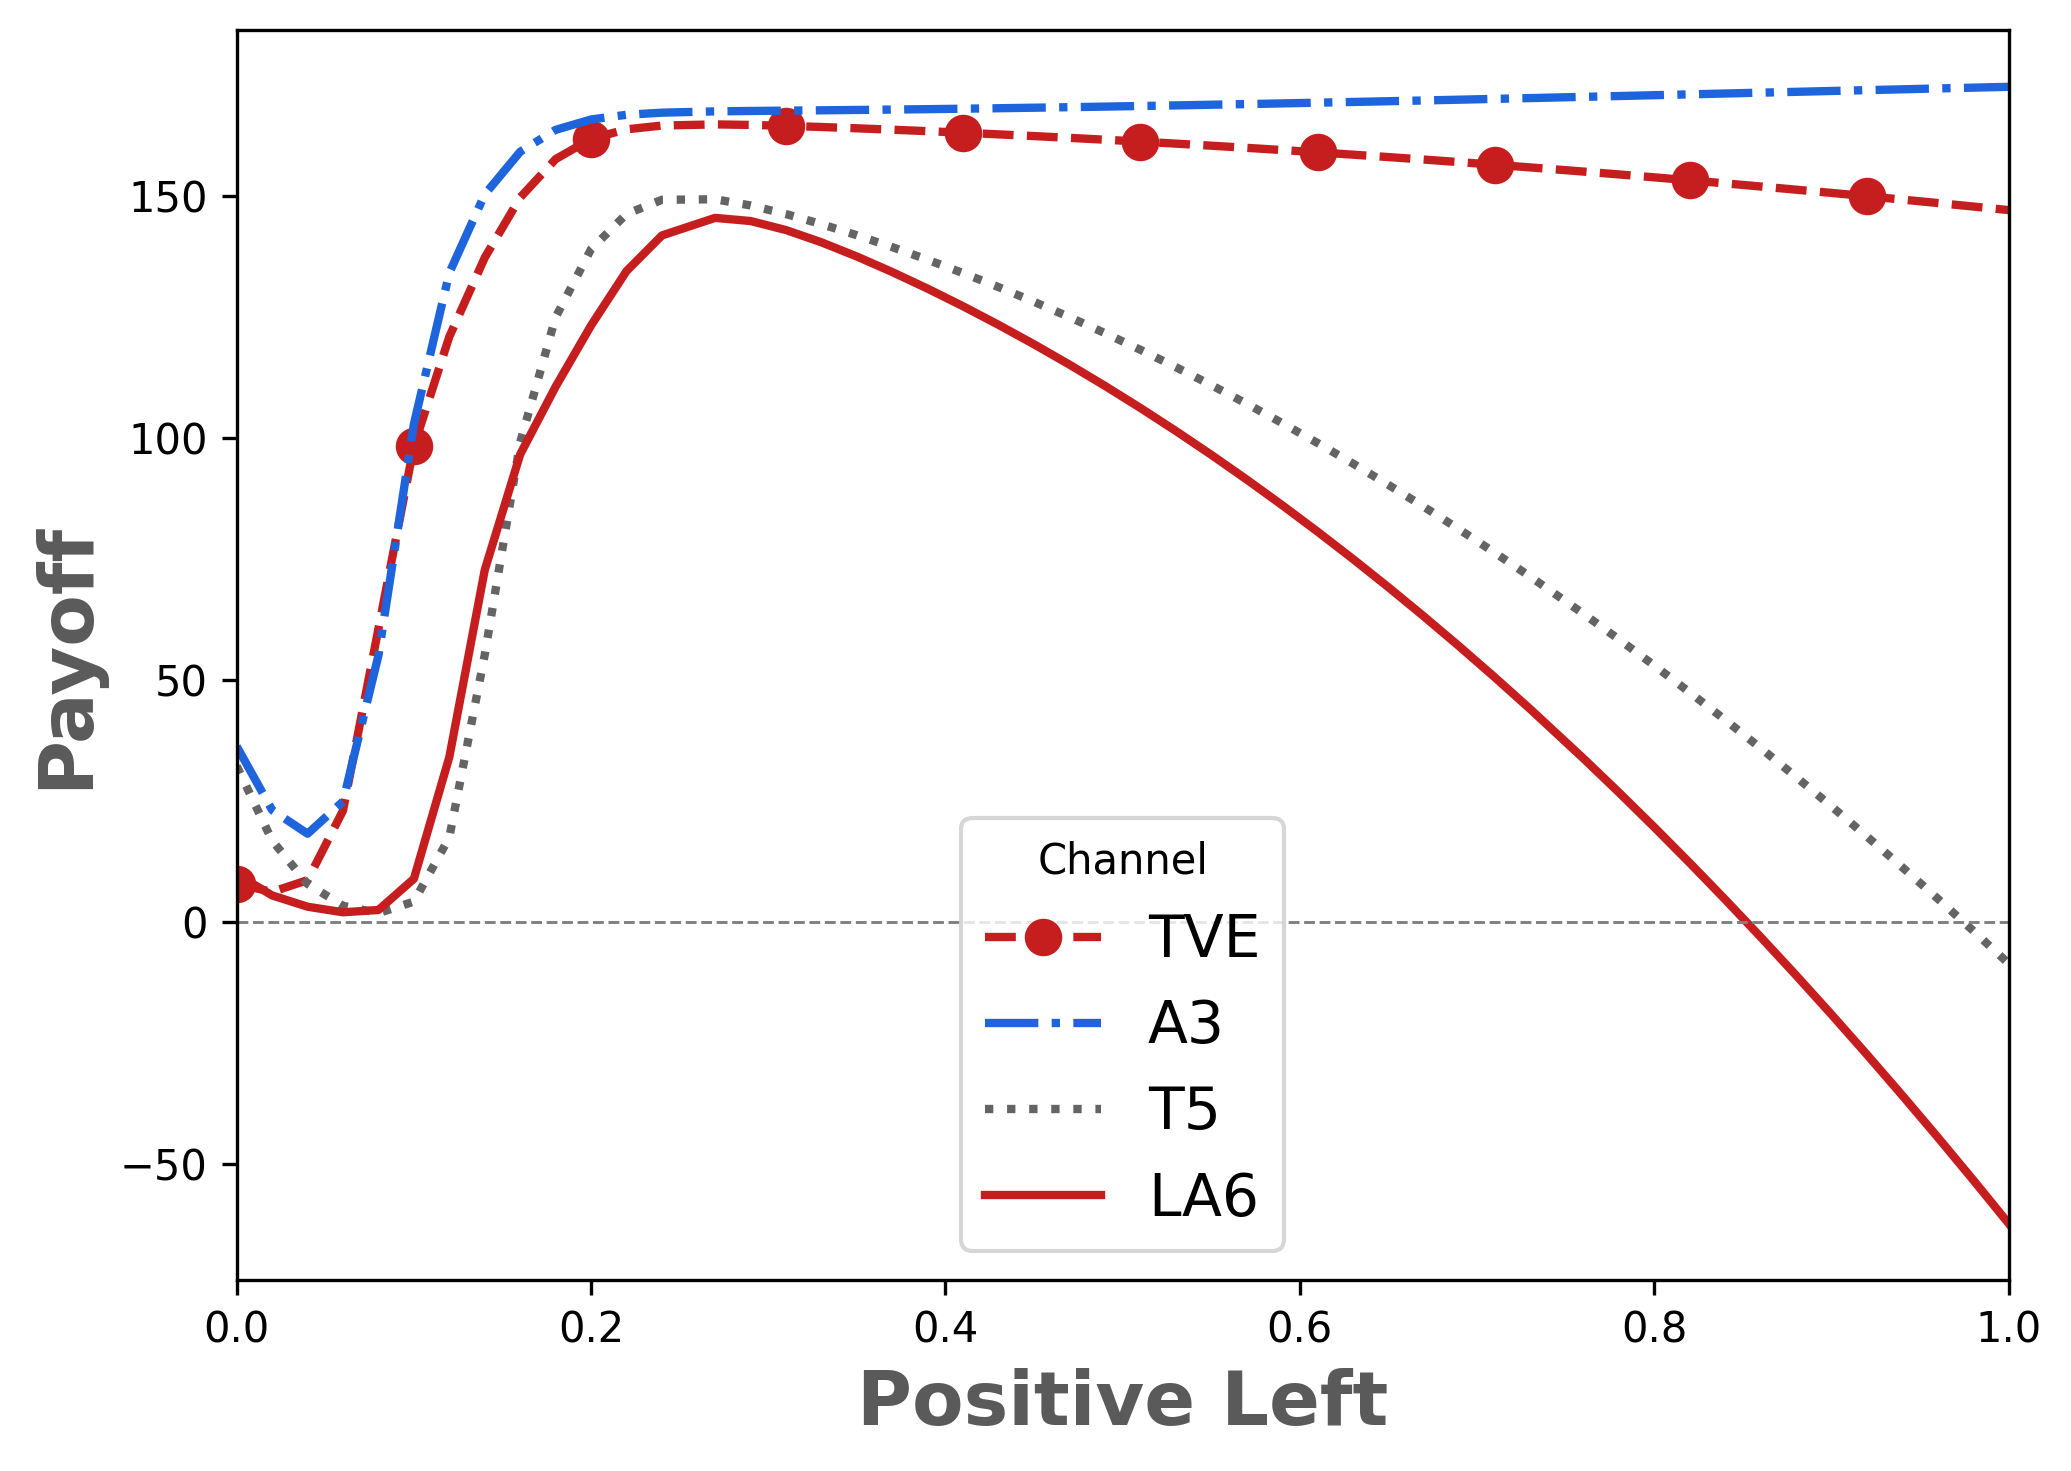
\includegraphics[width=0.45\textwidth]{figures/payoff_pos_left_all_positive} &
			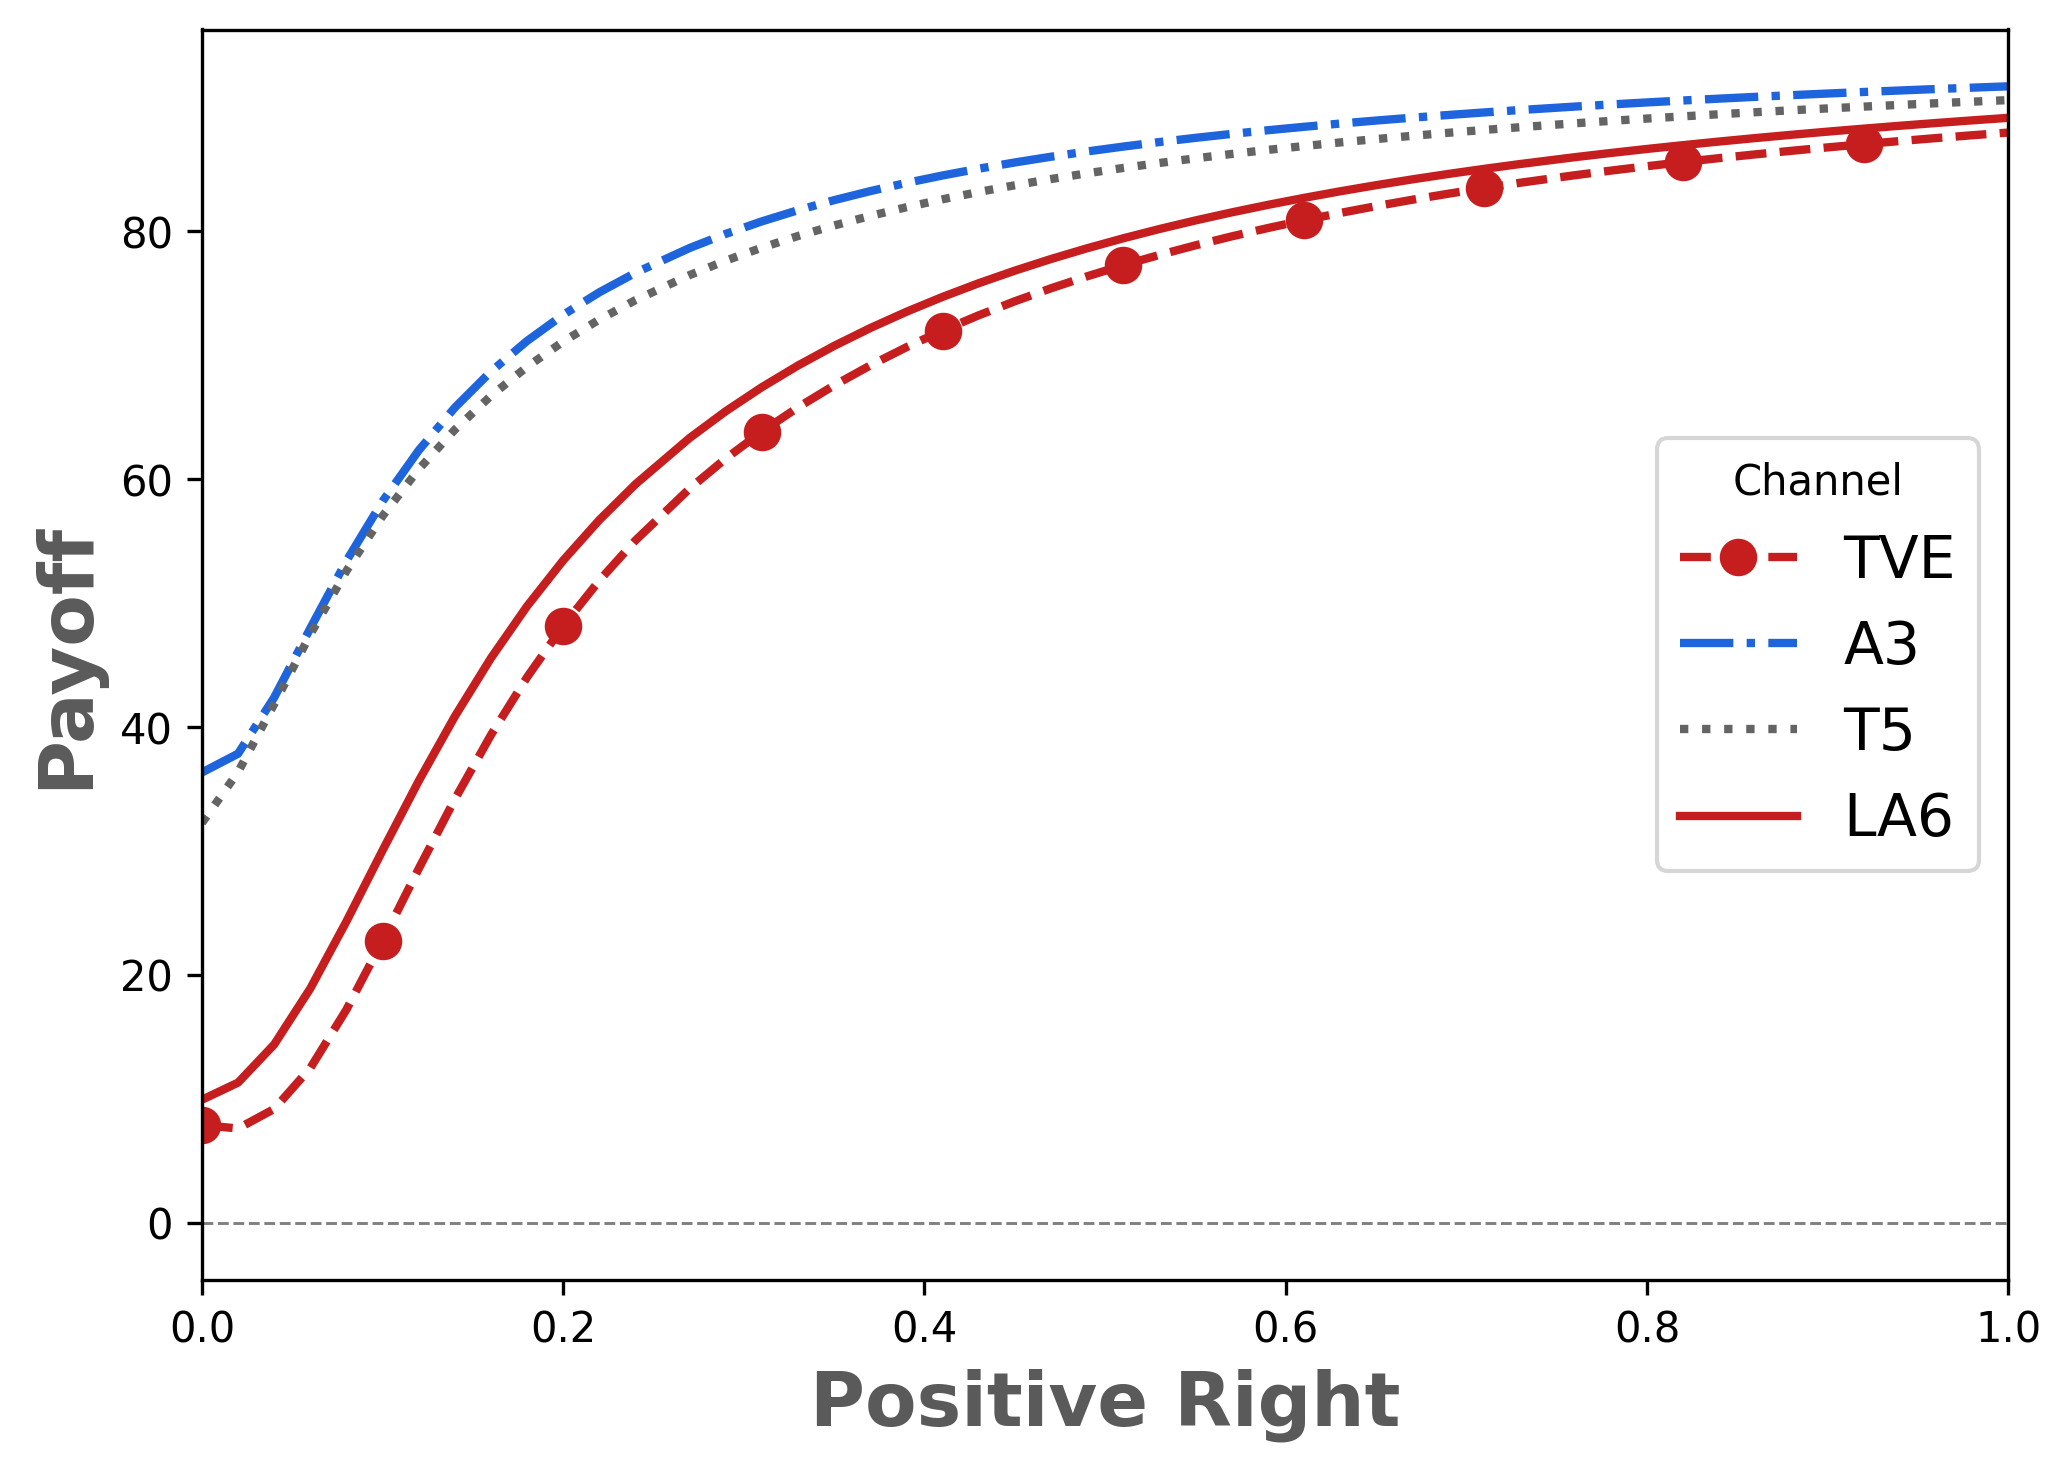
\includegraphics[width=0.45\textwidth]{figures/payoff_pos_right_all_positive} \\[1em]
			% Panel headers row
			\text{(c) Negative Left} &
			\text{(d) Negative Right} \\[0.08em]
			% Second row of plots
			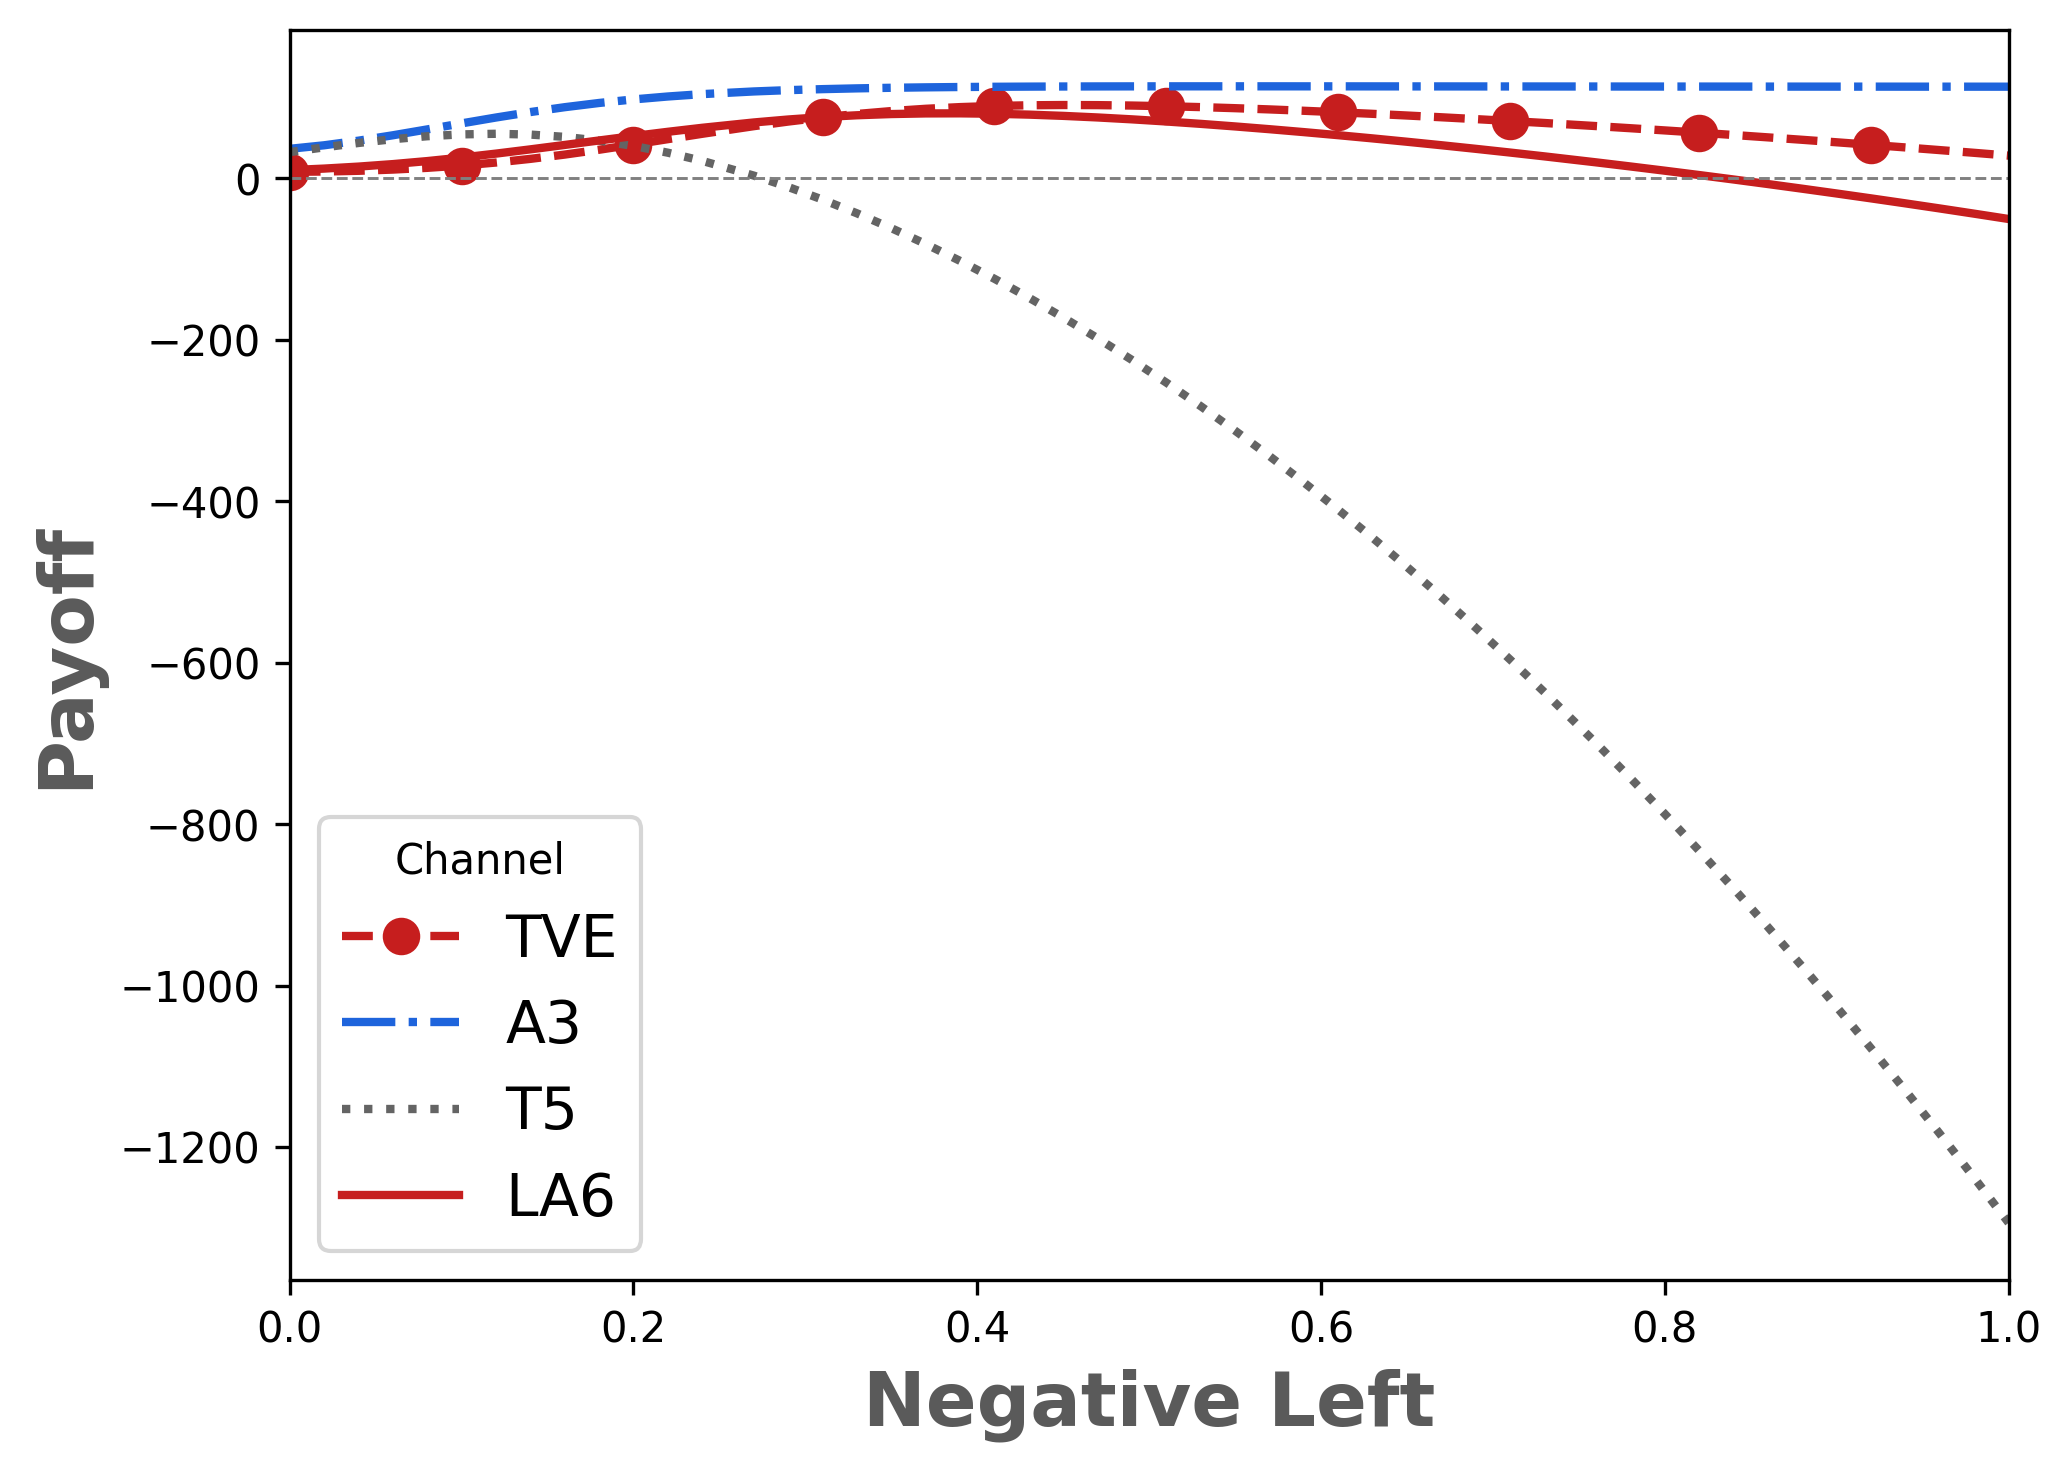
\includegraphics[width=0.45\textwidth]{figures/payoff_neg_left_all_positive} &
			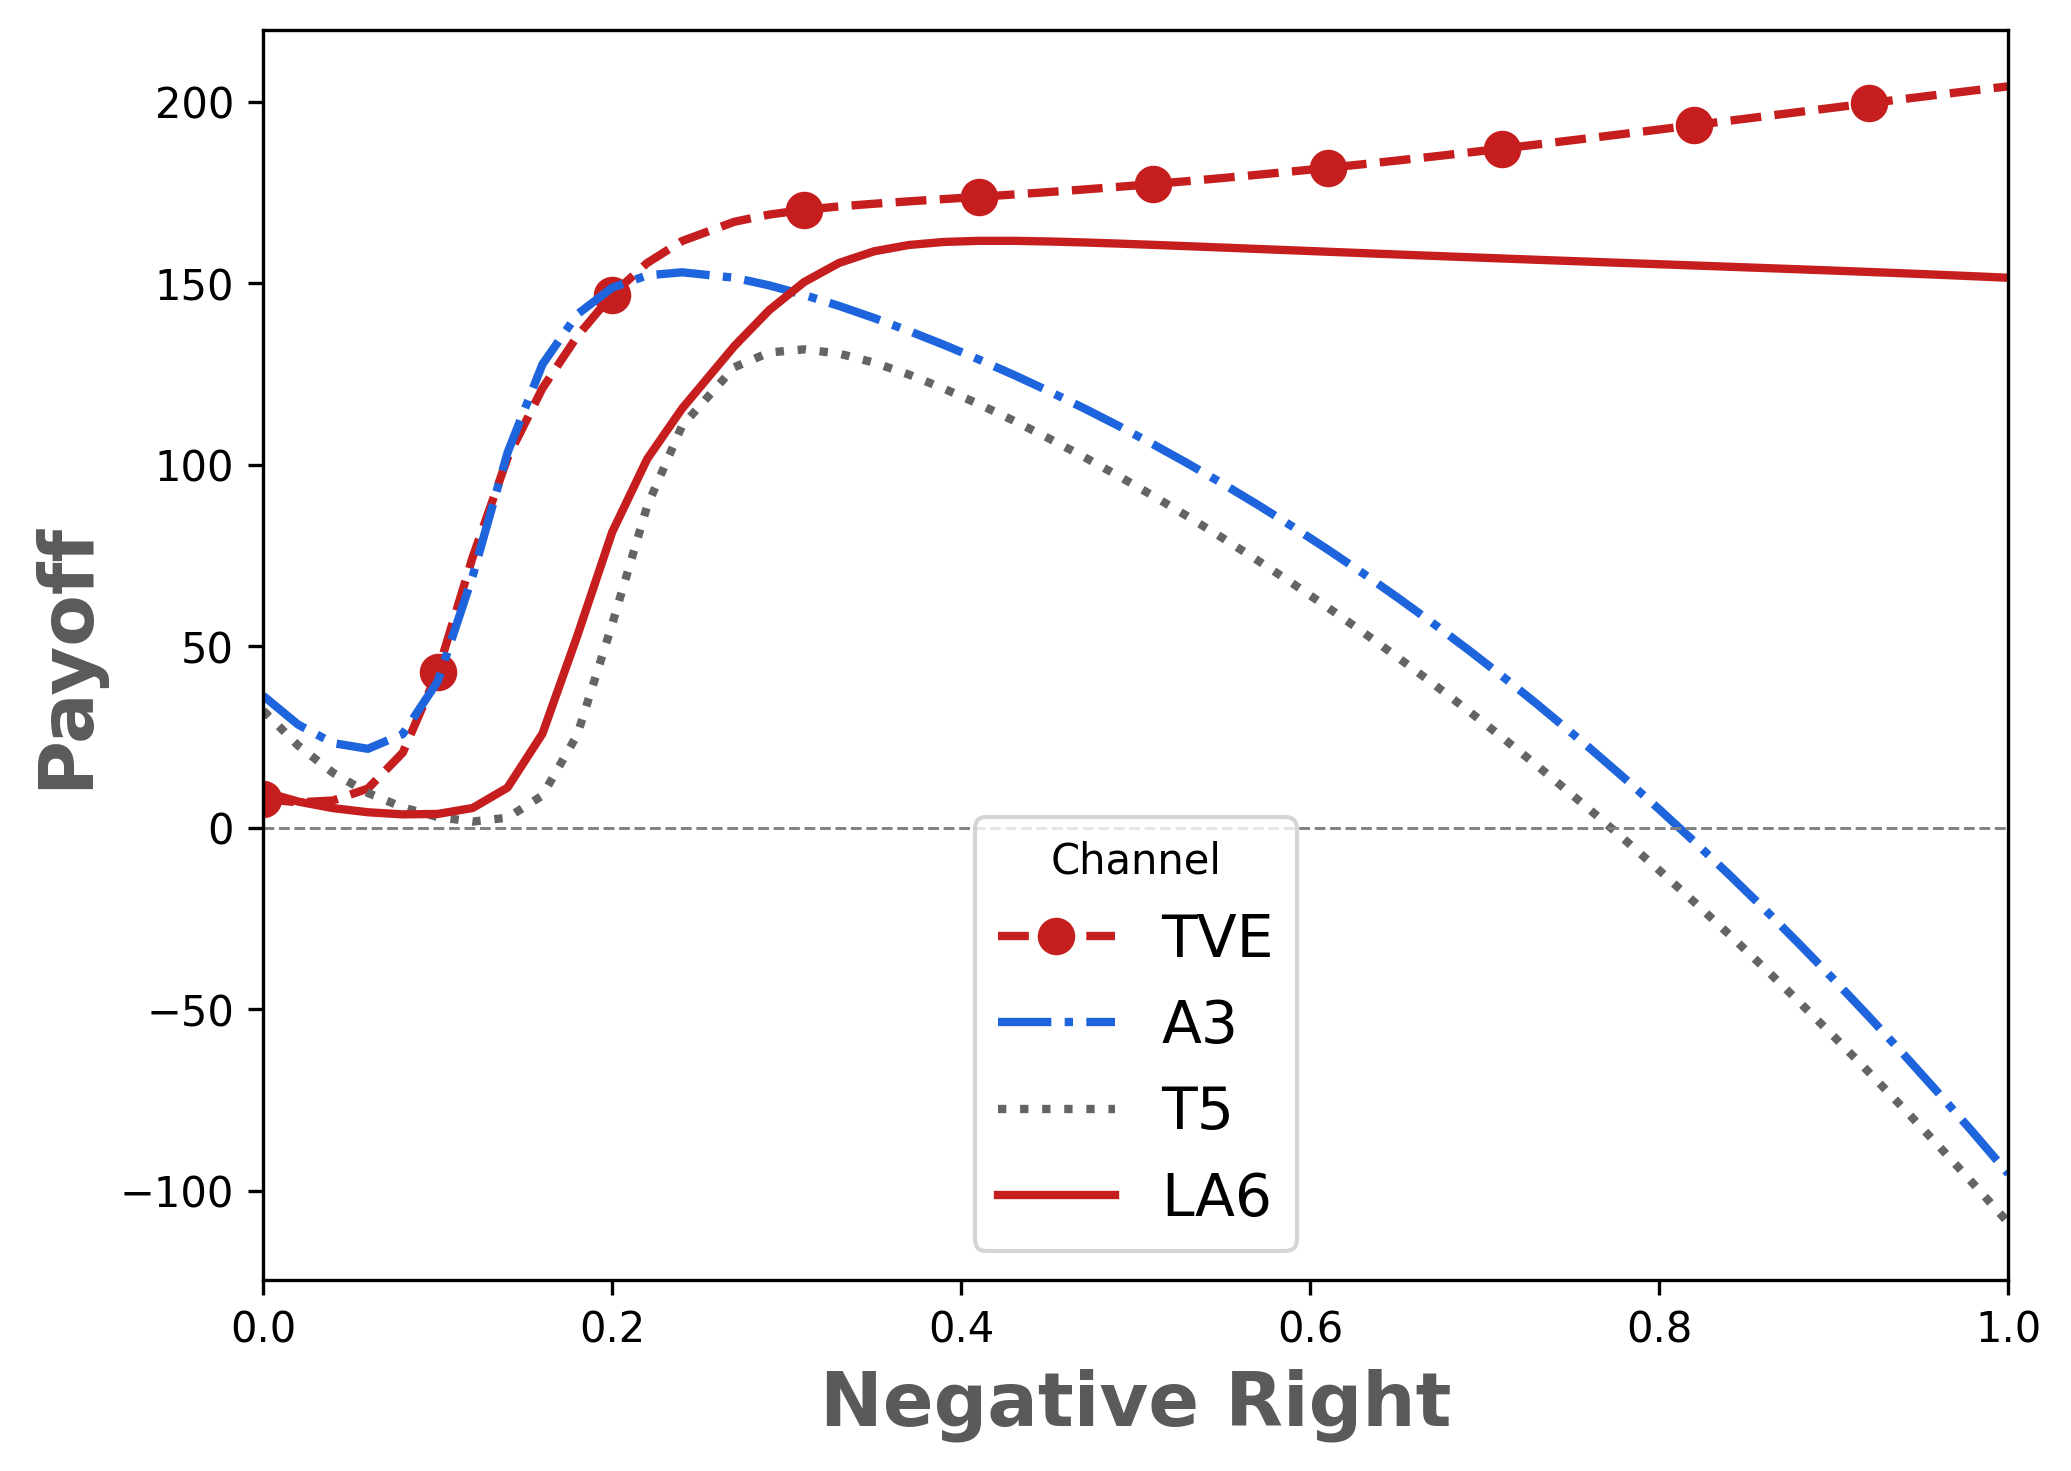
\includegraphics[width=0.45\textwidth]{figures/payoff_neg_right_all_positive}
		\end{tabular}
		\caption*{\small \textit{Note:} Figures shows the average payoffs of the supply game after estimation. y-axis values represent thousands of viewers. Average are taken over days. Each panel corresponds to one type of coverage: 
			(a) positive-left, (b) positive-right, (c) negative-left, and (d) negative-right.}
		\label{fig:payoffs_constrained}
	\end{figure}
	
	\begin{comment}
		content...

	\begin{figure}[ht]
		\centering
		\caption{Normalized Ideology Scores by Channel}
		% Panel (a): ChatGPT-based
		\begin{minipage}[t]{0.48\textwidth}
			\centering
			\textit{(a) Demand: Viewers' Elasticities}
			\includegraphics[width=\linewidth]{figures/congress_line_audience_share}
		\end{minipage}
		\hfill
		% Panel (b): CIS-based
		\begin{minipage}[t]{0.48\textwidth}
			\centering
			
			
			\textit{(b) Supply: ChatGPT text classification}
			\includegraphics[width=\linewidth]{figures/congress_line_chatgpt_campaign}
			
			
		\end{minipage}
		
		
		\caption*{\small \textit{Notes:} The figure compares normalized left–right audience positions for Spanish television channels. Panel (a) positions channels according to the demand elasticities from the BLP estimation. Panel (b) shows the relative  positions of the slant for the campaign according to the ChatGPT classification. 			Channels are mapped into the $[-1,1]$ scale with the two extreme ones forced into these values to compare across magnitudes.  }
		\label{fig:channel_ideology_lines2}
	\end{figure}
	
	
	\begin{figure}[ht!]
		\centering
		\caption{Political and Media Polarization (no-smoothing)}
		\includegraphics[width=150mm]{figures/er_polarization_stata_group_raw}
		\caption*{\textit{Note:} \small The figure shows the mean Esteban-Ray polarization index  computed as in equation \ref{eq:er}.  Solid (dashed) line represents the regions above (below) the median in terms of their media polarization consumption according to index \ref{eq:mediapol}.   }
		\label{fig:er}
	\end{figure}
	
		\end{comment}
	
	
	\begin{figure}[!htb]
		\centering
		\caption{Change in Positions Off-campaign to Campaign}
		\includegraphics[width=100mm]{figures/congress_line_chatgpt_pre_postv2}
		
		\caption*{\small \textit{Note:} The figure shows the relative change in  slant positions  according to the ideological index in Equation \eqref{eq:ideo_index} from off-campaign to campaign. 	}% Values are normalized so that the two most extreme positions take values -1 and 1 in the off-campaign period. }
	\label{fig:change_line}
	\end{figure}
	
	
	
	
	\begin{figure}[!htb]
		\centering
		\caption{Change in Positions Baseline vs Counterfactual Scenario}
		\includegraphics[width=100mm]{figures/congress_line_counter}
		
		\caption*{\small \textit{Note:} The figure shows the relative change in  slant positions  according to the ideological index in Equation \eqref{eq:ideo_index} from the factual to the counterfactual scenario during the campaign period.}
		\label{fig:change_line_counter}
	\end{figure}
	
	
	
	
	\clearpage

\section{Tables}
	
	\begin{comment}
		content...

	
	\begin{table}[!htbp]
		\centering
		\caption{Pearson Correlation of Ideology Index  with EFE}
		\begin{tabular}{lcc}
			\toprule
			\textbf{Channel} & \textbf{Political} & \textbf{Ideology Index} \\
			\midrule
			A3 & 0.666 & 0.364 \\
			T5 & 0.487 & 0.018 \\
			TVE & 0.381 & 0.320 \\
			La Sexta & 0.266 & 0.240 \\
			\bottomrule
		\end{tabular}
		\caption*{\small \textit{Note:} Pearson correlation coefficients ($r$) for the time series of political coverage and the ideology index  in Equation \ref{eq:ideo_index} between each TV channel and Agencia EFE.}
		\label{tab:correlations}
	\end{table}
	
		\end{comment}
	
	\subsection{Descriptive Evidence}
	
	
	
	\begin{table}[!htbp]
		\centering
		\caption{Proportion of Political Content and Sentiment by Channel}
		\begin{tabular}{llcc}
			\toprule
			\textbf{Outlet} & \textbf{Category} & \textbf{Pre-campaign} & \textbf{During campaign} \\
			\midrule
			\midrule
			\multirow{5}{*}{\textbf{A3}}& Negative Left & 0.106 & 0.090 \\
			& Negative Right & 0.043 & 0.066 \\
			& Positive Left & 0.065 & 0.061 \\
			& Positive Right & 0.023 & 0.039 \\
			& Political & 0.277 & 0.387 \\
			\midrule
			\multirow{5}{*}{\textbf{La Sexta}}& Negative Left & 0.041 & 0.032 \\
			& Negative Right & 0.047 & 0.067 \\
			& Positive Left & 0.049 & 0.057 \\
			& Positive Right & 0.013 & 0.012 \\
			& Political & 0.207 & 0.277 \\
			\midrule
			\multirow{5}{*}{\textbf{TVE}}& Negative Left & 0.038 & 0.037 \\
			& Negative Right & 0.045 & 0.046 \\
			& Positive Left & 0.072 & 0.052 \\
			& Positive Right & 0.012 & 0.021 \\
			& Political & 0.175 & 0.212 \\
			\midrule
			\multirow{5}{*}{\textbf{T5}}& Negative Left & 0.043 & 0.039 \\
			& Negative Right & 0.025 & 0.044 \\
			& Positive Left & 0.047 & 0.046 \\
			& Positive Right & 0.012 & 0.026 \\
			& Political & 0.111 & 0.183 \\
			\bottomrule
				\multirow{5}{*}{\textbf{ EFE}} & Negative Left & 0.076 & 0.073 \\
			& Negative Right & 0.058 & 0.094\\
			& Positive Left & 0.138 & 0.145 \\
			& Positive Right & 0.043 & 0.099\\
			& Political & 0.438 & 0.515 \\
			\bottomrule
			
		\end{tabular}
		\caption*{\small \textit{Note:} The table shows the proportion of political minutes and the breakdown by tone/party for each channel, off- and during campaign. For EFE it shows the proportion of stories of each category (Eqs. \eqref{eq:controls}). }
		\label{tab:political_sentiment_types}
	\end{table}
	
	
	
	
	\begin{table}[!htbp]
		\centering
		\caption{Proportion of Positive/Negative Minutes by Channel}
		\begin{tabular}{llcc}
			\toprule
			\textbf{Outlet} & \textbf{Category} & \textbf{Pre-campaign} & \textbf{During campaign} \\
			\midrule
			\midrule
			\multirow{4}{*}{\textbf{A3}} & Positive Left & 0.065 & 0.061 \\
			& Positive Right & 0.023 & 0.039 \\
			& Negative Left & 0.106 & 0.090 \\
			& Negative Right & 0.043 & 0.066 \\
			\midrule
			\multirow{4}{*}{\textbf{La Sexta}} & Positive Left & 0.049 & 0.057 \\
			& Positive Right & 0.013 & 0.012 \\
			& Negative Left & 0.041 & 0.032 \\
			& Negative Right & 0.047 & 0.067 \\
			\midrule
			\multirow{4}{*}{\textbf{T5}} & Positive Left & 0.047 & 0.046 \\
			& Positive Right & 0.012 & 0.026 \\
			& Negative Left & 0.043 & 0.039 \\
			& Negative Right & 0.025 & 0.044 \\
			\midrule
			\multirow{4}{*}{\textbf{TVE}} & Positive Left & 0.072 & 0.052 \\
			& Positive Right & 0.012 & 0.021 \\
			& Negative Left & 0.038 & 0.037 \\
			& Negative Right & 0.045 & 0.046 \\
			\midrule
			\bottomrule
		\end{tabular}
		\caption*{\small \textit{Note:} The table shows the proportion of positive and negative minutes for each channel, off- and during campaign  (Eqs. \eqref{eq:controls}.}
		\label{tab:positive_negative_minutes}
	\end{table}
	
	
	\FloatBarrier
	
	
	\subsection{Additional Results}
	
	

	


\begin{table}[!htb]
	\centering
	\caption{Estimated Elasticities}
	\begin{tabular}{lcc}
		\toprule
		Characteristic & \textbf{Pre-campaign}& \textbf{Campaign} \\
		\midrule
		Positive Right & 0.036 & -0.531 \\
		Negative Right & 1.012 & 0.070 \\
		Net Right (Positive - Negative) & -0.976 & -0.601 \\
		\hline
		Positive Left & 0.006 & -0.062 \\
		Negative Left & 1.009 & -0.150 \\
		Net Left (Positive - Negative) & -1.003 & 0.088 \\
		\bottomrule
	\end{tabular}
	\caption*{\textit{Note:} \small The table shows the average elasticities for each characteristic in Eq. \eqref{eq:elasticities}. }
	\label{tab:elasticities0}
\end{table}





\begin{table}[!htb]
	\centering
	\caption{Estimated Elasticities for Right and Left Markets}
	\begin{tabular}{l|cc|cc}
		\toprule
		& \multicolumn{2}{c|}{Pre-campaign} & \multicolumn{2}{c}{Campaign} \\
		Characteristic & Left Market & Right Market & Left Market & Right Market \\
		\midrule
		Negative Left & 1.705 & 0.313 & -0.747 & 0.333 \\
		& (0.022) & (0.005) & (0.093) & (0.044) \\
		Positive Left & -0.073 & 0.085 & 0.666 & -0.819 \\
		& (0.002) & (0.001) & (0.102) & (0.099) \\
		Negative Right & 1.443 & 0.580 & 0.277 & -0.164 \\
		& (0.019) & (0.008) & (0.065) & (0.032) \\
		Positive Right & -0.036 & 0.108 & -1.388 & 0.204 \\
		& (0.002) & (0.002) & (0.182) & (0.052) \\
		\bottomrule
	\end{tabular}
	\caption*{\textit{Note:} \small The table shows the average elasticities for each characteristic by right and left markets as defined in Eq. \eqref{eq:elasticities}. Right markets are defined as regions with proportion of right-wing voters above the median. Standard errors in parentheses are calculated as the standard error of the mean across markets.}
	\label{tab:elasticities}
\end{table}




\begin{table}[!htbp]\centering
	\footnotesize
\caption{Audience Compositional Change Tests}
\label{tab:compositional}
	\begin{threeparttable}
		\begin{tabular}{lcccccccccc|cc}
			\toprule
			& \multicolumn{10}{c}{\textbf{Age}} & \multicolumn{2}{c}{\textbf{Sex}} \\
			\cmidrule(lr){2-11}\cmidrule(lr){12-13}
			\textbf{Channel} & 4-9 & 10-12 & 13-15 & 16-24 & 25-29 & 30-34 & 35-44 & 45-54 & 55-64 & 65+ & Female & Male \\
			\midrule
			TVE & \shortstack{-0.03\\(0.67)} & \shortstack{-0.12\\(0.66)} & \shortstack{-0.07\\(0.63)} & \shortstack{0.19\\(0.52)} & \shortstack{0.18\\(0.66)} & \shortstack{0.11\\(0.63)} & \shortstack{-0.03\\(0.63)} & \shortstack{0.00\\(0.56)} & \shortstack{0.03\\(0.52)} & \shortstack{-0.07\\(0.47)} & \shortstack{-0.04\\(0.53)} & \shortstack{0.03\\(0.50)} \\
			A3 & \shortstack{-0.24\\(0.63)} & \shortstack{0.03\\(0.52)} & \shortstack{-0.34\\(0.49)} & \shortstack{-0.13\\(0.53)} & \shortstack{0.06\\(0.54)} & \shortstack{-0.05\\(0.49)} & \shortstack{-0.09\\(0.51)} & \shortstack{-0.09\\(0.49)} & \shortstack{-0.06\\(0.45)} & \shortstack{-0.02\\(0.43)} & \shortstack{-0.05\\(0.45)} & \shortstack{-0.02\\(0.47)} \\
			T5 & \shortstack{0.15\\(0.73)} & \shortstack{-0.00\\(0.70)} & \shortstack{0.03\\(0.63)} & \shortstack{0.01\\(0.63)} & \shortstack{-0.23\\(0.67)} & \shortstack{-0.18\\(0.63)} & \shortstack{0.15\\(0.58)} & \shortstack{0.05\\(0.61)} & \shortstack{0.15\\(0.65)} & \shortstack{0.06\\(0.65)} & \shortstack{0.07\\(0.59)} & \shortstack{0.06\\(0.71)} \\
			La Sexta & \shortstack{-0.21\\(1.03)} & \shortstack{-0.78\\(1.22)} & \shortstack{-0.20\\(0.93)} & \shortstack{-0.10\\(0.87)} & \shortstack{0.07\\(0.82)} & \shortstack{0.43\\(0.68)} & \shortstack{0.12\\(0.69)} & \shortstack{0.05\\(0.66)} & \shortstack{0.03\\(0.69)} & \shortstack{0.02\\(0.77)} & \shortstack{0.04\\(0.80)} & \shortstack{0.05\\(0.67)} \\
			\bottomrule
		\end{tabular}
		\begin{tablenotes}\footnotesize
			\item \textit{Notes:} Each cell reports the campaign profile coefficient from a logit testing audience share changes from the off- to the campaign periods. Robust standard errors in parentheses. 
		\end{tablenotes}
	\end{threeparttable}
\end{table}






\begin{table}[!htb]
	\centering
	\caption{Estimated Elasticities for Right and Left Markets (Baselline and Counterfactual)}
	\begin{tabular}{l|cc|cc}
		\toprule
		& \multicolumn{2}{c|}{Baseline} & \multicolumn{2}{c}{Counterfactual} \\
		Characteristic & Left Market & Right Market & Left Market & Right Market \\
		\midrule
		Negative Left & -0.747 & 0.333 & -6.742 & 2.163 \\
		Positive Left & 0.666 & -0.819 & 1.255 & -2.407 \\
		Negative Right & 0.277 & -0.164 & 3.950 & -5.726 \\
		Positive Right & -1.388 & 0.204 & -0.158 & 0.043 \\
		\bottomrule
	\end{tabular}
	\caption*{\textit{Note:} \small The table shows the average elasticities for each characteristic by right and left markets as defined in Eq.~\eqref{eq:elasticities}. Right markets are defined as regions with proportion of right-wing voters above the median. Left column shows the elasticities from the model estimation and the right column from the counterfactual Problem \eqref{eq:payoffs2}.}
	\label{tab:elasticities_count}
\end{table}

	
	
	
	
	
	\begin{comment}
		
		
		
		\begin{table}[!htb]
			\centering
			
			\caption{Effect of Mentions on Tone toward Party Leaders}
			\label{tab:images2}
			\small
			\setlength{\tabcolsep}{4pt}
			\renewcommand{\arraystretch}{1.0}
			\begin{tabular}{lcccc}
				\toprule
				& \multicolumn{4}{c}{\textit{Outlet Slant} (\(x\))} \\
				\cmidrule(lr){2-5}
				& (1) & (2) & (3) & (4) \\
				\midrule
				
				\multicolumn{5}{l}{\textbf{Feijóo (PP)}}\\
				Text Mentions     &  -1.956         &  -3.038         &   0.364         &   -1.342        \\
				&  (2.063)        &  (2.134)        &  (2.391)        &  (2.584)        \\
				Image Appearances &  -0.065         &   0.003         &  -0.275         &  -0.189         \\
				&  (0.147)        &  (0.151)        &  (0.179)        &  (0.189)        \\
				\addlinespace
				\hline
				\multicolumn{5}{l}{\textbf{Abascal (VOX)}}\\
				Text Mentions     & -42.813\sym{***}& -44.024\sym{***}& -46.659\sym{***}& -49.989\sym{***}\\
				&  (7.855)        &  (7.832)        &  (9.609)        &  (9.471)        \\
				Image Appearances &   0.963\sym{**} &   0.933\sym{**} &   0.565         &   0.437         \\
				&  (0.470)        &  (0.470)        &  (0.600)        &  (0.595)        \\
				\addlinespace
				\hline
				\multicolumn{5}{l}{\textbf{Sánchez (PSOE)}}\\
				Text Mentions     &   4.131         &  11.634\sym{*}  &   2.648         &  13.515\sym{*}  \\
				&  (6.020)        &  (6.992)        &  (6.494)        &  (7.909)        \\
				Image Appearances &   0.023         &  -0.045         &   0.033         &   0.032         \\
				&  (0.239)        &  (0.244)        &  (0.356)        &  (0.377)        \\
				\addlinespace
				\hline
				\multicolumn{5}{l}{\textbf{Díaz (UP)}}\\
				Text Mentions     &  -0.576         &   1.276         &  -0.714         &   3.365         \\
				&  (3.158)        &  (3.280)        &  (4.080)        &  (4.405)        \\
				Image Appearances &   0.473\sym{**} &   0.485\sym{**} &   0.290         &   0.321         \\
				&  (0.197)        &  (0.206)        &  (0.232)        &  (0.247)        \\
				\midrule
				Channel FE        & No              & Yes             & No              & Yes             \\
				Date FE           & No              & No              & Yes             & Yes             \\
				\midrule
				Observations      & 231             & 231             & 231             & 227             \\
				\bottomrule
			\end{tabular}
			
			\vspace{0.5em}
			\begin{flushleft}
				\scriptsize\emph{Note:} Robust standard errors in parentheses;\quad 
				\sym{*} \(p<0.05\), \sym{**} \(p<0.01\), \sym{***} \(p<0.001\).  
				Each block shows coefficients from regressing net tone on text mentions and image appearances of the party leader.
			\end{flushleft}
		\end{table}
		
		
This is the table when i run the regression separatedly without both controls on the same regression ( multicollinearity). 

	\begin{table}[!htb]
		\centering
		\caption{Effect of Mentions on Tone toward Party Leaders}
		\label{tab:images}
		\small
		\setlength{\tabcolsep}{4pt}
		\renewcommand{\arraystretch}{1.0}
		\begin{tabular}{lcccc}
			\toprule
			& \multicolumn{4}{c}{\textit{Outlet Slant} (\(x\))} \\
			\cmidrule(lr){2-5}
			& (1) No FE & (2) Channel FE & (3) Date FE & (4) Both FE \\
			\midrule
			
			\multicolumn{5}{l}{\textbf{Feijóo (PP)}}\\
			Text Mentions     &  -2.583         &  -3.145\sym{*}  &  -1.181         &  -2.112         \\
			&  (1.601)        &  (1.693)        &  (1.988)        &  (2.231)        \\
			Image Appearances &  -0.141         &  -0.109         &  -0.263         &  -0.222         \\
			&  (0.124)        &  (0.129)        &  (0.161)        &  (0.178)        \\
			\addlinespace
			\hline
			
			\multicolumn{5}{l}{\textbf{Abascal (Vox)}}\\
			Text Mentions     & -35.693\sym{***}& -37.210\sym{***}& -43.668\sym{***}& -46.976\sym{***}\\
			&  (6.742)        &  (6.725)        &  (8.891)        &  (8.843)        \\
			Image Appearances &  -0.093         &  -0.149         &  -0.039         &  -0.173         \\
			&  (0.455)        &  (0.457)        &  (0.625)        &  (0.630)        \\
			\addlinespace
			\hline
			
			\multicolumn{5}{l}{\textbf{Sánchez (PSOE)}}\\
			Text Mentions     &   4.359         &  11.306\sym{*}  &   1.957         &  12.359\sym{*}  \\
			&  (5.139)        &  (5.975)        &  (5.460)        &  (6.879)        \\
			Image Appearances &   0.096         &   0.135         &   0.088         &   0.236         \\
			&  (0.214)        &  (0.220)        &  (0.329)        &  (0.360)        \\
			\addlinespace
			\hline
			
			\multicolumn{5}{l}{\textbf{Díaz (UP)}}\\
			Text Mentions     &   2.739         &   4.778\sym{*}  &   0.993         &   5.037         \\
			&  (2.637)        &  (2.730)        &  (3.678)        &  (3.961)        \\
			Image Appearances &   0.456\sym{***}&   0.524\sym{***}&   0.277         &   0.381         \\
			&  (0.172)        &  (0.179)        &  (0.217)        &  (0.234)        \\
			\midrule
			Channel FE        & No              & Yes             & No              & Yes             \\
			Date FE           & No              & No              & Yes             & Yes             \\
			\midrule
			Observations      & 231             & 231             & 231             & 227             \\
			\bottomrule
		\end{tabular}
		
		\vspace{0.5em}
		\begin{flushleft}
			\scriptsize\emph{Note:} Robust standard errors in parentheses;\quad
			\sym{*} \(p<0.05\), \sym{**} \(p<0.01\), \sym{***} \(p<0.001\).  
			Each block reports the text‐only and image‐only coefficients under four FE specifications; Observations are from the image‐only models.
		\end{flushleft}
	\end{table}
	
		\end{comment}
	
	
	\begin{comment}
		content...

	
	
	\begin{table}[!htb]\centering
		\def\sym#1{\ifmmode^{#1}\else\(^{#1}\)\fi}
		\caption{Effect of Mentions on Tone toward Feijóo}
		\begin{tabular}{l*{4}{c}}
			\hline\hline
				\multicolumn{1}{c}{} & \multicolumn{4}{c}{\textit{Outlet Slant $(x)$}} \\ 
			\cline{2-5}
			&\multicolumn{1}{c}{(1)}         &\multicolumn{1}{c}{(2)}         &\multicolumn{1}{c}{(3)}         &\multicolumn{1}{c}{(4)}         \\
			\hline
			Text Mentions   &  -25.763         &  -51.515         &   42.517         &    6.957         \\
			& (50.044)         & (51.028)         & (61.383)         & (64.934)         \\
			Image Appearances  &   -4.373         &   -2.024         &  -12.421\sym{**} &   -9.379\sym{*}  \\
			&  (3.785)         &  (3.852)         &  (4.815)         &  (5.112)         \\
			constant          &   -0.088         &   -0.093         &   -0.049         &   -0.053         \\
			&  (0.076)         &  (0.077)         &  (0.093)         &  (0.101)         \\
			Channel FE      &       No         &      Yes         &       No         &      Yes         \\
			Date FE         &       No         &       No         &      Yes         &      Yes         \\
			\hline
			Observations    &      238         &      238         &      234         &      234         \\
			\hline\hline
		\end{tabular}
		\label{tab:feijoo_images}
		\vspace{0.5em}
		\caption*{\scriptsize\emph{Note:} Robust standard errors in parentheses. The table shows the estimated coefficients for a regression of net tone on the People's Party calculated as in \ref{eq:controls}, on the proportion of image appearances and text mentions of its party leader, Feijoo. Results are for a random sample of 67 days. }
	\end{table}
	
	
	\begin{table}[!htb]\centering
		\def\sym#1{\ifmmode^{#1}\else\(^{#1}\)\fi}
		\caption{Effect of Mentions on Tone toward Abascal}
		\begin{tabular}{l*{4}{c}}
			\hline\hline
				\multicolumn{1}{c}{} & \multicolumn{4}{c}{\textit{Outlet Slant $(x)$}} \\ 
			\cline{2-5}
			&\multicolumn{1}{c}{(1)}         &\multicolumn{1}{c}{(2)}         &\multicolumn{1}{c}{(3)}         &\multicolumn{1}{c}{(4)}         \\
			\hline
			Text Mentions   & -506.623\sym{***}& -534.081\sym{***}& -539.867\sym{***}& -609.038\sym{***}\\
			&(148.973)         &(147.122)         &(161.979)         &(156.866)         \\
			Image Appearances  &   18.013\sym{**} &   15.994\sym{*}  &   22.023\sym{**} &   17.193\sym{*}  \\
			&  (9.077)         &  (8.996)         & (10.119)         &  (9.898)         \\
			constant          &   -0.122\sym{**} &   -0.109\sym{*}  &   -0.130\sym{**} &   -0.099\sym{*}  \\
			&  (0.057)         &  (0.056)         &  (0.057)         &  (0.056)         \\
			Channel FE      &       No         &      Yes         &       No         &      Yes         \\
			Date FE         &       No         &       No         &      Yes         &      Yes         \\
			\hline
			Observations    &      238         &      238         &      234         &      234         \\
			\hline\hline
		\end{tabular}
		\label{tab:abascal_images}
		\vspace{0.5em}
		\caption*{\scriptsize\emph{Note:} Robust standard errors in parentheses. The table shows the estimated coefficients for a regression of net tone on VOX calculated as in \ref{eq:controls}, on the proportion of image appearances and text mentions of its party leader, Abascal. Results are for a random sample of 67 days. }
	\end{table}
	
	
	\begin{table}[!htb]\centering
		\def\sym#1{\ifmmode^{#1}\else\(^{#1}\)\fi}
		\caption{Effect of Mentions on Tone toward Sánchez}
		\begin{tabular}{l*{4}{c}}
			\hline\hline
				\multicolumn{1}{c}{} & \multicolumn{4}{c}{\textit{Outlet Slant $(x)$}} \\ 
			\cline{2-5}
			&\multicolumn{1}{c}{(1)}         &\multicolumn{1}{c}{(2)}         &\multicolumn{1}{c}{(3)}         &\multicolumn{1}{c}{(4)}         \\
			\hline
			Text Mentions   &   61.471         &  196.424         &   27.282         &  193.827         \\
			&(106.565)         &(123.145)         &(119.969)         &(145.161)         \\
			Image Appearances  &   -2.352         &   -4.286         &   -7.639         &  -10.754         \\
			&  (4.253)         &  (4.331)         &  (6.583)         &  (6.971)         \\
			constant          &    0.054         &    0.014         &    0.120         &    0.077         \\
			&  (0.063)         &  (0.067)         &  (0.075)         &  (0.085)         \\
			Channel FE      &       No         &      Yes         &       No         &      Yes         \\
			Date FE         &       No         &       No         &      Yes         &      Yes         \\
			\hline
			Observations    &      238         &      238         &      234         &      234         \\
			\hline\hline
		\end{tabular}
		\label{tab:sanchez_images}
		\vspace{0.5em}
		\caption*{\scriptsize\emph{Note:} Robust standard errors in parentheses. The table shows the estimated coefficients for a regression of net tone on PSOE calculated as in \ref{eq:controls}, on the proportion of image appearances and text mentions of its party leader, Sánchez. Results are for a random sample of 67 days. }
	\end{table}
	
	
	\begin{table}[!htb]\centering
		\def\sym#1{\ifmmode^{#1}\else\(^{#1}\)\fi}
		\caption{Effect of Mentions on Tone toward Díaz}
		\begin{tabular}{l*{4}{c}}
			\hline\hline
				\multicolumn{1}{c}{} & \multicolumn{4}{c}{\textit{Outlet Slant $(x)$}} \\ 
			\cline{2-5}
			&\multicolumn{1}{c}{(1)}         &\multicolumn{1}{c}{(2)}         &\multicolumn{1}{c}{(3)}         &\multicolumn{1}{c}{(4)}         \\
			\hline
			Text Mentions   &  -11.990         &   21.235         &  -78.607         &  -19.353         \\
			& (67.519)         & (69.918)         & (91.794)         & (99.632)         \\
			Image Appearances  &    0.019         &   -0.072         &   -0.861         &   -1.032\sym{*}  \\
			&  (0.512)         &  (0.517)         &  (0.595)         &  (0.603)         \\
			constant          &    0.064         &    0.051         &    0.103\sym{**} &    0.080         \\
			&  (0.044)         &  (0.045)         &  (0.051)         &  (0.054)         \\
			Channel FE      &       No         &      Yes         &       No         &      Yes         \\
			Date FE         &       No         &       No         &      Yes         &      Yes         \\
			\hline
			Observations    &      238         &      238         &      234         &      234         \\
			\hline\hline
		\end{tabular}
		\label{tab:diaz_images}
		\vspace{0.5em}
		\caption*{\scriptsize\emph{Note:} Robust standard errors in parentheses. The table shows the estimated coefficients for a regression of net tone on UP calculated as in \ref{eq:controls}, on the proportion of image appearances and text mentions of its party leader, Díaz. Results are for a random sample of 67 days. }
	\end{table}
	
	

	
	\begin{table}[htbp]
		\centering
		\scriptsize
		\setlength{\tabcolsep}{4pt}
		\renewcommand{\arraystretch}{0.9}
		\caption{First Stage Regressions}
		\label{tab:first_stage}
		\begin{tabular}{lcccc}
		\hline
		% span columns 2–5 (the four slant columns)
		\multicolumn{1}{c}{} & \multicolumn{4}{c}{\textit{Outlet Slant $(x)$}} \\ 
		\cline{2-5}
		& \textbf{(1) Positive Right}
		& \textbf{(2) Negative Right}
		& \textbf{(3) Positive Left}
		& \textbf{(4) Negative Left} \\
		\hline
			
			% Single grouping header
			\multicolumn{5}{l}{\textit{News‐Shock $(z)$}}\\
			\hline
			
			% Now only the short block names
			\multicolumn{5}{l}{\textbf{Positive Right}}\\
			\hline
			TVE            &  0.00342         & -0.00456         & -0.0498         & -0.0916         \\
			&  (0.08)          & (-0.07)          & (-0.71)         & (-1.30)         \\
			A3             &  0.207\sym{***}  & -0.139           & -0.0615         & -0.113          \\
			&  (4.62)          & (-1.89)          & (-0.81)         & (-1.47)         \\
			T5             & -0.0372          & -0.0746          & -0.0943         & -0.166\sym{*}   \\
			& (-0.88)          & (-1.08)          & (-1.31)         & (-2.28)         \\
			La Sexta       &  0.0334          & -0.0129          &  0.0290         & -0.0256         \\
			&  (0.73)          & (-0.17)          &  (0.37)         & (-0.33)         \\
			\hline
			
			\multicolumn{5}{l}{\textbf{Negative Right}}\\
			\hline
			TVE            & -0.0296          &  0.00590         & -0.0707         &  0.0738         \\
			& (-0.74)          &  (0.09)          & (-1.04)         &  (1.08)         \\
			A3             & -0.0333          &  0.0929          & -0.0104         & -0.0440         \\
			& (-0.79)          &  (1.34)          & (-0.14)         & (-0.61)         \\
			T5             & -0.0585          &  0.131           &  0.0327         & -0.0166         \\
			& (-1.05)          &  (1.44)          &  (0.35)         & (-0.17)         \\
			La Sexta       & -0.0185          &  0.143\sym{*}    & -0.0399         & -0.123          \\
			& (-0.42)          &  (1.97)          & (-0.53)         & (-1.63)         \\
			\hline
			
			\multicolumn{5}{l}{\textbf{Positive Left}}\\
			\hline
			TVE            &  0.0261         &  0.0634         &  0.200\sym{**}  & -0.0511         \\
			&  (0.68)         &  (1.01)         &  (3.07)         & (-0.78)         \\
			A3             &  0.00911        & -0.0626         &  0.0154         & -0.0845         \\
			&  (0.22)         & (-0.92)         &  (0.22)         & (-1.19)         \\
			T5             & -0.0712         & -0.159          & -0.00405        & -0.0572         \\
			& (-1.43)         & (-1.95)         & (-0.05)         & (-0.67)         \\
			La Sexta       &  0.00655        & -0.0906         & -0.00875        &  0.0718         \\
			&  (0.16)         & (-1.33)         & (-0.12)         &  (1.01)         \\
			\hline
			
			\multicolumn{5}{l}{\textbf{Negative Left}}\\
			\hline
			TVE            &  0.0144         & -0.0603         & -0.176\sym{*}   &  0.149          \\
			&  (0.32)         & (-0.81)         & (-2.26)         &  (1.90)         \\
			A3             &  0.0446         & -0.133          & -0.173\sym{*}   &  0.184\sym{*}   \\
			&  (0.93)         & (-1.69)         & (-2.11)         &  (2.23)         \\
			T5             & -0.141\sym{**}  &  0.0136         & -0.00461        & -0.0569         \\
			& (-2.66)         &  (0.16)         & (-0.05)         & (-0.63)         \\
			La Sexta       &  0.0262         & -0.141          & -0.139          &  0.111          \\
			&  (0.53)         & (-1.73)         & (-1.65)         &  (1.31)         \\
			\hline\hline
		\end{tabular}
		\caption*{\scriptsize\emph{Note:} Robust standard errors in parentheses; \sym{*} $p<0.05$, \sym{**} $p<0.01$, \sym{***} $p<0.001$. Total observations: $N=687$.}
	\end{table}
	
	\begin{table}[htbp]
		\centering
		\scriptsize
		\setlength{\tabcolsep}{4pt}
		\renewcommand{\arraystretch}{0.9}
		\caption{First Stage Regressions}
		\label{tab:first_stage}
		\begin{tabular}{lcccc}
			\hline
			\multicolumn{1}{c}{} & \multicolumn{4}{c}{\textit{Outlet Slant $(x)$}} \\ 
			\cline{2-5}
			& \textbf{(1) Positive Right}
			& \textbf{(2) Negative Right}
			& \textbf{(3) Positive Left}
			& \textbf{(4) Negative Left} \\
			\hline
			
			\multicolumn{5}{l}{\textit{News‐Shock $(z)$}}\\
			\hline
			
			\multicolumn{5}{l}{\textbf{Positive Right}}\\
			\hline
			TVE            &  0.00342         & -0.00456         & -0.0498         & -0.0916         \\
			&  (0.0409)        & (0.0672)         & (0.0698)        & (0.0703)        \\
			A3             &  0.207\sym{***}  & -0.139           & -0.0615         & -0.113          \\
			&  (0.0448)        & (0.0736)         & (0.0764)        & (0.0769)        \\
			T5             & -0.0372          & -0.0746          & -0.0943         & -0.166\sym{*}   \\
			&  (0.0423)        & (0.0694)         & (0.0721)        & (0.0726)        \\
			La Sexta       &  0.0334          & -0.0129          &  0.0290         & -0.0256         \\
			&  (0.0455)        & (0.0747)         & (0.0775)        & (0.0781)        \\
			\hline
			
			\multicolumn{5}{l}{\textbf{Negative Right}}\\
			\hline
			TVE            & -0.0296          &  0.00590         & -0.0707         &  0.0738         \\
			&  (0.0397)        & (0.0652)         & (0.0677)        & (0.0682)        \\
			A3             & -0.0333          &  0.0929          & -0.0104         & -0.0440         \\
			&  (0.0423)        & (0.0694)         & (0.0721)        & (0.0726)        \\
			T5             & -0.0585          &  0.131           &  0.0327         & -0.0166         \\
			&  (0.0555)        & (0.0910)         & (0.0945)        & (0.0952)        \\
			La Sexta       & -0.0185          &  0.143\sym{*}    & -0.0399         & -0.123          \\
			&  (0.0441)        & (0.0725)         & (0.0752)        & (0.0758)        \\
			\hline
			
			\multicolumn{5}{l}{\textbf{Positive Left}}\\
			\hline
			TVE            &  0.0261          &  0.0634          &  0.200\sym{**}  & -0.0511         \\
			&  (0.0382)        & (0.0627)         & (0.0651)        & (0.0655)        \\
			A3             &  0.00911         & -0.0626          &  0.0154         & -0.0845         \\
			&  (0.0414)        & (0.0680)         & (0.0706)        & (0.0711)        \\
			T5             & -0.0712          & -0.159          & -0.00405        & -0.0572         \\
			&  (0.0497)        & (0.0815)         & (0.0846)        & (0.0852)        \\
			La Sexta       &  0.00655         & -0.0906          & -0.00875        &  0.0718         \\
			&  (0.0416)        & (0.0683)         & (0.0709)        & (0.0714)        \\
			\hline
			
			\multicolumn{5}{l}{\textbf{Negative Left}}\\
			\hline
			TVE            &  0.0144          & -0.0603          & -0.176\sym{*}   &  0.149          \\
			&  (0.0455)        & (0.0748)         & (0.0776)        & (0.0782)        \\
			A3             &  0.0446          & -0.133           & -0.173\sym{*}   &  0.184\sym{*}   \\
			&  (0.0481)        & (0.0790)         & (0.0820)        & (0.0826)        \\
			T5             & -0.141\sym{**}   &  0.0136          & -0.00461        & -0.0569         \\
			&  (0.0529)        & (0.0868)         & (0.0901)        & (0.0908)        \\
			La Sexta       &  0.0262          & -0.141           & -0.139          &  0.111          \\
			&  (0.0495)        & (0.0812)         & (0.0843)        & (0.0849)        \\
			\hline
			
			\multicolumn{5}{l}{\textbf{Political}}\\
			\hline
			TVE            &  0.0167          &  0.0680\sym{*}   &  0.0828\sym{*}  &  0.0494         \\
			&  (0.0204)        & (0.0335)         & (0.0348)        & (0.0350)        \\
			A3             &  0.0187          &  0.145\sym{***}  &  0.137\sym{***} &  0.175\sym{***} \\
			&  (0.0222)        & (0.0364)         & (0.0378)        & (0.0381)        \\
			T5             &  0.0975\sym{***} &  0.0981\sym{*}   &  0.0837         &  0.125\sym{**}  \\
			&  (0.0264)        & (0.0434)         & (0.0451)        & (0.0454)        \\
			La Sexta       &  0.0145          &  0.132\sym{***}  &  0.123\sym{**}  &  0.0393         \\
			&  (0.0231)        & (0.0380)         & (0.0394)        & (0.0397)        \\
			\hline\hline
		\end{tabular}
		\caption*{\small \textit{Note:} Results of the estimation of the regression equation  \eqref{eq:first_stage}.
			Robust standard errors in parentheses; 
			$p<0.1$, \sym{*} $p<0.05$, \sym{**} $p<0.01$, \sym{***} $p<0.001$. 
			Total observations: $N=687$.}
	\end{table}
	
			\end{comment}
	

	
	
	\begin{table}[htbp]
		\centering
		\scriptsize
		\setlength{\tabcolsep}{4pt}
		\renewcommand{\arraystretch}{0.9}
		\caption{First Stage Regressions for Demand}
		\label{tab:first_stage}
		\begin{tabular}{lcccc}
			\hline
			\multicolumn{1}{c}{} & \textbf{(1) Positive Right} & \textbf{(2) Negative Right} & \textbf{(3) Positive Left} & \textbf{(4) Negative Left} \\
			\hline
			
			\multicolumn{5}{l}{\textit{News‐Shock $(z)$}}\\
			\hline
			
			\multicolumn{5}{l}{\textbf{Positive Right}}\\
			\hline
			TVE       & -0.0246       & 0.0104        & 0.0507        & -0.0856       \\
			& (0.0506)      & (0.0837)      & (0.0855)      & (0.0862)      \\
			A3        & 0.244\sym{***}& -0.0395       & 0.0732        & 0.0118        \\
			& (0.0538)      & (0.0889)      & (0.091)       & (0.0917)      \\
			T5        & 0.0499        & 0.0539        & -0.0688       & -0.114        \\
			& (0.0572)      & (0.0945)      & (0.0966)      & (0.0974)      \\
			La Sexta  & -0.0283       & 0.0556        & 0.0818        & -0.108        \\
			& (0.0535)      & (0.0884)      & (0.0904)      & (0.0912)      \\
			\hline
			
			\multicolumn{5}{l}{\textbf{Negative Right}}\\
			\hline
			TVE       & -0.0407       & 0.0604        & -0.0641       & 0.0283        \\
			& (0.0425)      & (0.0702)      & (0.0718)      & (0.0724)      \\
			A3        & 0.0175        & 0.166\sym{*}  & 0.0126        & -0.00300      \\
			& (0.0477)      & (0.0787)      & (0.081)       & (0.0812)      \\
			T5        & -0.0530       & 0.199\sym{*}  & 0.0769        & 0.0466        \\
			& (0.0562)      & (0.0929)      & (0.095)       & (0.0957)      \\
			La Sexta  & -0.0281       & 0.179\sym{**} & -0.0266       & -0.224\sym{**}\\
			& (0.0465)      & (0.0769)      & (0.0786)      & (0.0792)      \\
			\hline
			
			\multicolumn{5}{l}{\textbf{Positive Left}}\\
			\hline
			TVE       & 0.0498        & 0.253\sym{***}& 0.394\sym{***}& 0.122         \\
			& (0.0446)      & (0.0737)      & (0.0754)      & (0.0760)      \\
			A3        & 0.154\sym{**} & 0.0572        & 0.132         & 0.202\sym{*}  \\
			& (0.0468)      & (0.0773)      & (0.0790)      & (0.0797)      \\
			T5        & 0.00992       & 0.0324        & 0.126         & 0.126         \\
			& (0.0589)      & (0.0974)      & (0.0996)      & (0.100)       \\
			La Sexta  & -0.0536       & -0.0424       & 0.118         & 0.0943        \\
			& (0.0472)      & (0.0780)      & (0.0797)      & (0.0804)      \\
			\hline
			
			\multicolumn{5}{l}{\textbf{Negative Left}}\\
			\hline
			TVE       & 0.0829        & 0.119         & -0.00250      & 0.344\sym{***}\\
			& (0.0520)      & (0.0859)      & (0.0878)      & (0.0885)      \\
			A3        & 0.174\sym{**} & 0.00666       & -0.0501       & 0.492\sym{***}\\
			& (0.0570)      & (0.0941)      & (0.0962)      & (0.0970)      \\
			T5        & -0.0649       & 0.167\sym{*}  & 0.0275        & 0.182\sym{*}  \\
			& (0.0606)      & (0.100)       & (0.102)       & (0.103)       \\
			La Sexta  & -0.0519       & -0.0869       & -0.0741       & 0.187\sym{*}  \\
			& (0.0581)      & (0.096)       & (0.0981)      & (0.099)       \\
			\hline
			
			\multicolumn{5}{l}{\textbf{Political}}\\
			\hline
			TVE       & -0.00269      & -0.0666       & -0.0470       & -0.0686       \\
			& (0.0287)      & (0.0475)      & (0.0485)      & (0.0489)      \\
			A3        & -0.0883\sym{**}& 0.0295       & 0.0418        & -0.0496       \\
			& (0.0308)      & (0.0509)      & (0.0520)      & (0.0524)      \\
			T5        & 0.0468        & -0.0543       & 0.00609       & -0.0231       \\
			& (0.0360)      & (0.0595)      & (0.0608)      & (0.0613)      \\
			La Sexta  & 0.0653\sym{*} & 0.0738        & 0.0506        & 0.0445        \\
			& (0.0306)      & (0.0505)      & (0.0516)      & (0.0521)      \\
			\hline\hline
			\textbf{R$^2$} & 0.3539 & 0.5025 & 0.5511 & 0.5573 \\
			\hline\hline
		\end{tabular}
		\caption*{\small \textit{Note:} Robust standard errors in parentheses. 
			$p<0.05$, \sym{*} $p<0.01$, \sym{**} $p<0.001$, \sym{***}. 
			Total observations: $N=687$.}
	\end{table}
	
	
	
\begin{comment}
	
	
		\begin{table}[htbp]
		\centering
		\scriptsize
		\setlength{\tabcolsep}{4pt}
		\renewcommand{\arraystretch}{0.9}
		\caption{First Stage Regressions}
		\label{tab:first_stage}
		\begin{tabular}{lcccc}
			\hline
			\multicolumn{1}{c}{} & \multicolumn{4}{c}{\textit{Outlet Slant $(x)$}} \\ 
			\cline{2-5}
			& \textbf{(1) Positive Right}
			& \textbf{(2) Negative Right}
			& \textbf{(3) Positive Left}
			& \textbf{(4) Negative Left} \\
			\hline
			
			\multicolumn{5}{l}{\textit{News‐Shock $(z)$}}\\
			\hline
			
			\multicolumn{5}{l}{\textbf{Positive Right}}\\
			\hline
			TVE            &  0.00342         & -0.00456         & -0.0498         & -0.0916         \\
			&  (0.08)          & (-0.07)          & (-0.71)         & (-1.30)         \\
			A3             &  0.207\sym{***}  & -0.139           & -0.0615         & -0.113          \\
			&  (4.62)          & (-1.89)          & (-0.81)         & (-1.47)         \\
			T5             & -0.0372          & -0.0746          & -0.0943         & -0.166\sym{*}   \\
			& (-0.88)          & (-1.08)          & (-1.31)         & (-2.28)         \\
			La Sexta       &  0.0334          & -0.0129          &  0.0290         & -0.0256         \\
			&  (0.73)          & (-0.17)          &  (0.37)         & (-0.33)         \\
			\hline
			
			\multicolumn{5}{l}{\textbf{Negative Right}}\\
			\hline
			TVE            & -0.0296          &  0.00590         & -0.0707         &  0.0738         \\
			& (-0.74)          &  (0.09)          & (-1.04)         &  (1.08)         \\
			A3             & -0.0333          &  0.0929          & -0.0104         & -0.0440         \\
			& (-0.79)          &  (1.34)          & (-0.14)         & (-0.61)         \\
			T5             & -0.0585          &  0.131           &  0.0327         & -0.0166         \\
			& (-1.05)          &  (1.44)          &  (0.35)         & (-0.17)         \\
			La Sexta       & -0.0185          &  0.143\sym{*}    & -0.0399         & -0.123          \\
			& (-0.42)          &  (1.97)          & (-0.53)         & (-1.63)         \\
			\hline
			
			\multicolumn{5}{l}{\textbf{Positive Left}}\\
			\hline
			TVE            &  0.0261         &  0.0634         &  0.200\sym{**}  & -0.0511         \\
			&  (0.68)         &  (1.01)         &  (3.07)         & (-0.78)         \\
			A3             &  0.00911        & -0.0626         &  0.0154         & -0.0845         \\
			&  (0.22)         & (-0.92)         &  (0.22)         & (-1.19)         \\
			T5             & -0.0712         & -0.159          & -0.00405        & -0.0572         \\
			& (-1.43)         & (-1.95)         & (-0.05)         & (-0.67)         \\
			La Sexta       &  0.00655        & -0.0906         & -0.00875        &  0.0718         \\
			&  (0.16)         & (-1.33)         & (-0.12)         &  (1.01)         \\
			\hline
			
			\multicolumn{5}{l}{\textbf{Negative Left}}\\
			\hline
			TVE            &  0.0144         & -0.0603         & -0.176\sym{*}   &  0.149          \\
			&  (0.32)         & (-0.81)         & (-2.26)         &  (1.90)         \\
			A3             &  0.0446         & -0.133          & -0.173\sym{*}   &  0.184\sym{*}   \\
			&  (0.93)         & (-1.69)         & (-2.11)         &  (2.23)         \\
			T5             & -0.141\sym{**}  &  0.0136         & -0.00461        & -0.0569         \\
			& (-2.66)         &  (0.16)         & (-0.05)         & (-0.63)         \\
			La Sexta       &  0.0262         & -0.141          & -0.139          &  0.111          \\
			&  (0.53)         & (-1.73)         & (-1.65)         &  (1.31)         \\
			\hline
			
			\multicolumn{5}{l}{\textbf{Political}}\\
			\hline
			TVE            &  0.0167         &  0.0680\sym{*}   &  0.0828\sym{*}  &  0.0494         \\
			&  (0.82)         &  (2.03)         &  (2.38)         &  (1.41)         \\
			A3             &  0.0187         &  0.145\sym{***}  &  0.137\sym{***} &  0.175\sym{***} \\
			&  (0.84)         &  (3.98)         &  (3.62)         &  (4.59)         \\
			T5             &  0.0975\sym{***}&  0.0981\sym{*}   &  0.0837 &  0.125\sym{**}  \\
			&  (3.69)         &  (2.26)         &  (1.86)         &  (2.77)         \\
			La Sexta       &  0.0145         &  0.132\sym{***}  &  0.123\sym{**}  &  0.0393         \\
			&  (0.63)         &  (3.47)         &  (3.12)         &  (0.99)         \\
			\hline\hline
		\end{tabular}
		\caption*{\small \textit{Note:} Results of the estimation of the regression equation  \eqref{eq:first_stage}.
			Robust standard errors in parentheses; 
			$p<0.1$, \sym{*} $p<0.05$, \sym{**} $p<0.01$, \sym{***} $p<0.001$. 
			Total observations: $N=687$.}
	\end{table}
	
	
	
	


\begin{table}[htbp]
	\centering
	\scriptsize
	\setlength{\tabcolsep}{4pt}
	\renewcommand{\arraystretch}{0.9}
	\def\sym#1{\ifmmode^{#1}\else\(^{#1}\)\fi}
	\caption{First Stage Regressions}
	\label{tab:first_stage}
	\begin{tabular}{lcccc}
		\hline\hline
		& \multicolumn{1}{c}{(1) Positive Right}
		& \multicolumn{1}{c}{(2) Negative Right}
		& \multicolumn{1}{c}{(3) Positive Left}
		& \multicolumn{1}{c}{(4) Negative Left} \\
		\hline
		\multicolumn{5}{l}{\textbf{Positive Right (All)}}\\
				\hline
		TVE            &  0.00342         & -0.00456         & -0.0498         & -0.0916         \\
		&  (0.08)          & (-0.07)          & (-0.71)         & (-1.30)         \\
		A3             &  0.207\sym{***}  & -0.139           & -0.0615         & -0.113          \\
		&  (4.62)          & (-1.89)          & (-0.81)         & (-1.47)         \\
		T5             & -0.0372          & -0.0746          & -0.0943         & -0.166\sym{*}   \\
		& (-0.88)          & (-1.08)          & (-1.31)         & (-2.28)         \\
		La Sexta       &  0.0334          & -0.0129          &  0.0290         & -0.0256         \\
		&  (0.73)          & (-0.17)          &  (0.37)         & (-0.33)         \\
		\hline
		\multicolumn{5}{l}{\textbf{Negative Right (All)}}\\
				\hline
		TVE            & -0.0296          &  0.00590         & -0.0707         &  0.0738         \\
		& (-0.74)          &  (0.09)          & (-1.04)         &  (1.08)         \\
		A3             & -0.0333          &  0.0929          & -0.0104         & -0.0440         \\
		& (-0.79)          &  (1.34)          & (-0.14)         & (-0.61)         \\
		T5             & -0.0585          &  0.131           &  0.0327         & -0.0166         \\
		& (-1.05)          &  (1.44)          &  (0.35)         & (-0.17)         \\
		La Sexta       & -0.0185          &  0.143\sym{*}    & -0.0399         & -0.123          \\
		& (-0.42)          &  (1.97)          & (-0.53)         & (-1.63)         \\
		\hline
		\multicolumn{5}{l}{\textbf{Positive Left (All)}}\\
				\hline
		TVE            &  0.0261         &  0.0634         &  0.200\sym{**}  & -0.0511         \\
		&  (0.68)         &  (1.01)         &  (3.07)         & (-0.78)         \\
		A3             &  0.00911        & -0.0626         &  0.0154         & -0.0845         \\
		&  (0.22)         & (-0.92)         &  (0.22)         & (-1.19)         \\
		T5             & -0.0712         & -0.159          & -0.00405        & -0.0572         \\
		& (-1.43)         & (-1.95)         & (-0.05)         & (-0.67)         \\
		La Sexta       &  0.00655        & -0.0906         & -0.00875        &  0.0718         \\
		&  (0.16)         & (-1.33)         & (-0.12)         &  (1.01)         \\
		\hline
		\multicolumn{5}{l}{\textbf{Negative Left (All)}}\\
				\hline
		TVE            &  0.0144         & -0.0603         & -0.176\sym{*}   &  0.149          \\
		&  (0.32)         & (-0.81)         & (-2.26)         &  (1.90)         \\
		A3             &  0.0446         & -0.133          & -0.173\sym{*}   &  0.184\sym{*}   \\
		&  (0.93)         & (-1.69)         & (-2.11)         &  (2.23)         \\
		T5             & -0.141\sym{**}  &  0.0136         & -0.00461        & -0.0569         \\
		& (-2.66)         &  (0.16)         & (-0.05)         & (-0.63)         \\
		La Sexta       &  0.0262         & -0.141          & -0.139          &  0.111          \\
		&  (0.53)         & (-1.73)         & (-1.65)         &  (1.31)         \\
		\hline
		\multicolumn{5}{l}{\textbf{Political (All)}}\\
				\hline
		TVE            &  0.0167         &  0.0680\sym{*}  &  0.0828\sym{*}  &  0.0494         \\
		&  (0.82)         &  (2.03)         &  (2.38)         &  (1.41)         \\
		A3             &  0.0187         &  0.145\sym{***}&  0.137\sym{***}&  0.175\sym{***}\\
		&  (0.84)         &  (3.98)         &  (3.62)         &  (4.59)         \\
		T5             &  0.0975\sym{***}&  0.0981\sym{*}  &  0.0837         &  0.125\sym{**}  \\
		&  (3.69)         &  (2.26)         &  (1.86)         &  (2.77)         \\
		La Sexta       &  0.0145         &  0.132\sym{***}&  0.123\sym{**} &  0.0393         \\
		&  (0.63)         &  (3.47)         &  (3.12)         &  (0.99)         \\
		\hline\hline
	\end{tabular}
	
	\caption*{\scriptsize\emph{Note:} Robust standard errors in  parentheses;\quad \sym{*} $p<0.05$, \sym{**} $p<0.01$, \sym{***} $p<0.001$. The table shows the results of the first stage regressions in equation \ref{eq:first_stage}. The total number of observations is $N=687$ }
	

\end{table}

\end{comment}
	
	
	
	
	
	\begin{table}[!htb]
			\caption{Logit Estimation Results with Standard Errors}
		\label{tab:logit}
		\centering
		\begin{threeparttable}
			\begin{tabular}{lccc}
				\hline
				\textbf{Coefficient} & \textbf{Parameter} & \textbf{Estimate} & \textbf{Std.\ Error} \\
				\hline
				\hline
				\multicolumn{4}{c}{\textbf{Pre-campaign}} \\
				\hline
				Positive Left & $\beta^{L+}$ & -17.62 & (14.344) \\
				Positive Right & $\beta^{R+}$ & -41.16** & (18.718) \\
				Negative Left & $\beta^{L-}$ & 27.24 & (20.268) \\
				Negative Right & $\beta^{R-}$ & 66.04* & (34.668) \\
				Political & $\beta^{political}$ & 14.28* & (7.465) \\
				Weather & $\gamma$ & 0.01 & (0.655) \\
				Positive Left $\times$ Right-Mean & $\phi^{L+}$ & 47.67 & (36.262) \\
				Positive Right $\times$ Right-Mean & $\phi^{R+}$ & 111.13** & (50.798) \\
				Negative Left $\times$ Right-Mean & $\phi^{L-}$ & -81.40 & (51.195) \\
				Negative Right $\times$ Right-Mean & $\phi^{R-}$ & -151.24* & (89.249) \\
				Political $\times$ Right-Mean & $\phi^{political}$ & -30.80 & (18.952) \\
				\hline
				\hline
				\multicolumn{4}{c}{\textbf{Campaign}} \\
				\hline
				Positive Left & $\beta^{L+}$ & 222.18** & (110.419) \\
				Positive Right & $\beta^{R+}$ & -177.76** & (88.006) \\
				Negative Left & $\beta^{L-}$ & -153.39** & (76.074) \\
				Negative Right & $\beta^{R-}$ & 147.85** & (69.428) \\
				Political & $\beta^{political}$ & -10.37** & (5.107) \\
				Weather & $\gamma$ & 0.80*** & (0.287) \\
				Positive Left $\times$ Right-Mean & $\phi^{L+}$ & -619.77** & (303.679) \\
				Positive Right $\times$ Right-Mean & $\phi^{R+}$ & 461.19* & (242.882) \\
				Negative Left $\times$ Right-Mean & $\phi^{L-}$ & 398.26* & (211.132) \\
				Negative Right $\times$ Right-Mean & $\phi^{R-}$ & -413.87** & (187.584) \\
				Political $\times$ Right-Mean & $\phi^{political}$ & 28.91** & (14.181) \\
				\hline
			\end{tabular}

			
				\caption*{\small  \textit{Note:} The table shows the results of the logit estimation of model \eqref{eq:logit}. The estimations are divided into the off-campaign and campaign period. Both day-of-the-week and outlet fixed effects are included. Standard errors are clustered at the region level. The total number of observations are $N_{campaign}=2307$ and  $N_{pre\_campaign}=6604$.}
			
		\end{threeparttable}
	\end{table}
	
	\begin{comment}
		content...

	
\begin{table}[!htb]
	\centering
	\caption{Top 5 Topics by Party-Tone Category on Agencia EFE after BERTopic. }
	\begin{tabular}{|l|c|}
		\hline
				\multicolumn{1}{|c|}{\textbf{Topic Words}}& \textbf{Count} \\
		\hline
		\hline
		\multicolumn{2}{|c|}{\textbf{Positive Right}} \\
		\hline
		vox, motion, abascal, censure, pp, tamames, santiago, garriga, parties, party & 312 \\
		feijóo, núñez, alberto, pp, leader, gamarra, parties, party, general, cuca & 113 \\
		guardiola, extremadura, mérida, maría, vara, extremeño, council, assembly, candidate & 68 \\
		mazón, valencian, president, corts, valencian, valencians, government, carlos & 64 \\
		electoral, elections, general, jec, board, campaign, 28m, 23j, vote & 63 \\
		\hline
		\multicolumn{2}{|c|}{\textbf{Negative Right}} \\
		\hline
		vox, motion, abascal, censure, pp, tamames, santiago, garriga, parties, party & 369 \\
		abortion, castilla, healthcare, anti-abortion,pregnancy, abortions, law, mañueco & 112 \\
		code, criminal, sedition, embezzlement, reform, crime, penalties, amendments & 81 \\
		electoral, elections, general, jec, board, campaign, 28m, 23j, vote & 71 \\
		sánchez, pedro, feijóo, president, government, núñez, leader, alberto, pp, executive & 69 \\
		\hline
		\multicolumn{2}{|c|}{\textbf{Positive Left}} \\
		\hline
		yes, only, reform, sexual, law, is, violence, reform, just, podemos & 200 \\
		sánchez, pedro, feijóo, president, government, núñez, leader, alberto, pp, executive & 183 \\
		yolanda, díaz, vice president, sumar, second, podemos, labor, leader, minister & 179 \\
		sumar, podemos, errejón, iu, íñigo, yolanda, parties, coalition, díaz, left-wing & 142 \\
		psoe, socialists, federal, secretary, parties, socialist, lobato, espadas, congress & 129 \\
		\hline
		\multicolumn{2}{|c|}{\textbf{Negative Left}} \\
		\hline
		yes, only, reform, sexual, law, is, violence, reform, just, podemos & 182 \\
		sánchez, pedro, feijóo, president, government, núñez, leader, alberto, pp, executive & 153 \\
		vox, motion, abascal, censure, pp, tamames, santiago, garriga, parties, party & 129 \\
		sexual, assault, sexually, sexual, minor, violence, assault, convicted, abuse & 108 \\
		psoe, socialists, federal, secretary, parties, socialist, lobato, espadas, congress & 72 \\
		\hline
	\end{tabular}
	\caption{Table shows the top 5 topics associated with the top stories that provided more positive/negative coverage for each party in the Agencia EFE corpus. words were translated to English with the help of ChatGPT. }
\end{table}

		\end{comment}
	
	
	
	\begin{sidewaystable}[!htbp]
		\caption{Robustness for the Estimated Cost Parameters ($\lambda$) by Channel and Estimator}
		\label{tab:costs_robust}
		\centering\small
		\begin{tabular}{l|ccc|ccc|ccc|ccc|}
			\toprule
			& \multicolumn{3}{c|}{La~Sexta} & \multicolumn{3}{c|}{TVE} & \multicolumn{3}{c|}{Telecinco (T5)} & \multicolumn{3}{c|}{Antena~3 (A3)} \\
			& Unconstr. & NNLS & NLLS & Unconstr. & NNLS & NLLS & Unconstr. & NNLS & NLLS & Unconstr. & NNLS & NLLS \\
			\midrule
			Negative Left & 12.82 & 8.17 & 10.38 & 6.27 & 5.68 & 6.69 & 108.34 & 83.23 & 112.34 & -38.96 & 0.00 & 0.00 \\
			& (44.44) & (44.45) & (8.50) & (2.63) & (2.64) & (1.66) & (60.39) & (60.31) & (53.00) & (23.79) & (24.65) & (0.00) \\
			\midrule
			Positive Right & -89.09 & 0.00 & 0.00 & -103.74 & 0.00 & 0.00 & -13.87 & 0.00 & 0.00 & -240.52 & 0.00 & 0.00 \\
			& (85.99) & (97.60) & (0.00) & (121.36) & (112.30) & (0.00) & (91.62) & (88.67) & (0.00) & (77.50) & (94.67) & (0.00) \\
			\midrule
			Positive Left & 36.11 & 11.38 & 14.88 & 3.36 & 11.53 & 7.89 & 24.03 & 47.67 & 16.62 & -40.03 & 0.00 & 0.00 \\
			& (52.70) & (52.71) & (14.68) & (13.12) & (13.12) & (5.71) & (43.99) & (43.95) & (23.57) & (84.81) & (81.40) & (0.00) \\
			\midrule
			Negative Right & 4.07 & 0.00 & 2.62 & -8.88 & 2.21 & 0.00 & 31.13 & 38.43 & 25.78 & 35.16 & 2.71 & 4.44 \\
			& (4.80) & (4.80) & (1.86) & (11.41) & (11.39) & (0.00) & (36.16) & (36.27) & (26.73) & (53.89) & (53.70) & (20.13) \\
			\midrule
			Political & -0.35 & 0.00 & 0.00 & 0.32 & 0.21 & 0.23 & 1.50 & 1.39 & 1.64 & 1.45 & 0.52 & 0.00 \\
			& (0.61) & (0.60) & (0.00) & (0.62) & (0.65) & (0.21) & (1.05) & (1.13) & (0.87) & (1.25) & (1.36) & (0.00) \\
			\midrule
			\bottomrule
		\end{tabular}
		\vspace{0.5em}
		\caption*{\small \emph{Note:} Robust standard errors in parentheses. Each column shows the results under unconstrained GMM, non-negative least squares (NNLS), and nonlinear least squares (NLLS), respectively. }
	\end{sidewaystable}
	
	
\clearpage
	\subsection{Text Examples}
	
	
	
		\begin{table}[!htb]
								\caption{Top Stories for Negative Left and Outlet's Production}
		\centering
		\begin{tabular}{p{0.8\textwidth}}
			\toprule
			\textbf{Stories}  \\
			\midrule
			-Reduction of a convicted rapist’s sentence in Salamanca under the "Solo sí es sí" law  \\
			-Seville Court reduces a murder and sexual assault sentence by 5 years due to the "Solo sí es sí" law  \\
			-VOX formally submits a motion of no confidence against Prime Minister Pedro Sánchez  \\
			-Madrid’s regional president, Isabel Díaz Ayuso, predicts that the "Mediator Case" will bring down the government  \\
			\bottomrule
		\end{tabular}
		\begin{tabular}{l c}
			\toprule
			\textbf{Channel} & \textbf{Proportion of Negative Left} \\
			\midrule
			TVE & 0.037 \\
			A3  & 0.184 \\
			T5  & 0.037 \\
			La Sexta  & 0.01 \\
			\bottomrule
		\end{tabular}

		
					\caption*{\small  \textit{Note:} Top table shows the main stories contributing to negative left content on 2023-02-27, the highest day with negative left content,  summarized and translated to English by ChatGPT. Bottom table shows the proportion of minutes devoted to negative left content per channel on the same date.}
		
		\label{tab:neg_left_channels}
	\end{table}
	
	
		\begin{table}[!htb]
								\caption{Top Stories for Negative Right and Outlet's Production}
		\centering
		\begin{tabular}{p{0.8\textwidth}}
			\toprule
			\textbf{Stories}  \\
			\midrule
			-Congress declarations against Ayuso over alleged "bribes" to her brother  \\
			-Marinaleda criticizes the "abusive" arrest of two residents during a protest against Vox  \\
			-The Senate rejects a PP motion on the government's alleged partisan use of the Falcon jet  \\
			\bottomrule
		\end{tabular}
		\begin{tabular}{l c}
			\toprule
			\textbf{Channel} & \textbf{Proportion of Negative Right} \\
			\midrule
			TVE & 0.074 \\
			A3  & 0.038 \\
			T5 & 0.067 \\
			La Sexta  & 0.148 \\
			\bottomrule
		\end{tabular}

		
			\caption*{\small  \textit{Note:} Top table shows the main stories contributing to negative right content on 2023-05-17, the highest day with negative right content,  summarized and translated to English by ChatGPT. Bottom table shows the proportion of minutes devoted to negative right content per channel on the same date. }

		\label{tab:neg_right_channels}
	\end{table}
	
	
	\begin{comment}
	
	\begin{table}[!htb]
		\caption{Top trigrams for Positive Right and Negative Right in the Agencia EFE}
		\centering
		\begin{tabular}{|l|l|}
			\hline
			Positive Right & Negative Right \\
			\hline
			vox secretary general & gürtel national service \\
			vox ignacio garriga & gürtel trial service \\
			general vox ignacio & valencia francisco camps \\
			núñez feijóo called & gürtel trial gürtel \\
			pp candidate elections & former president valencian government \\
			vox parties madrid & valencian government francisco \\
			josé sáenz buruaga & psoe deputy secretary general \\
			núñez feijóo requested & gürtel trial madrid \\
			maría josé sáenz & abortion law reform \\
			may pp president & former valencian president francisco \\
			\hline
		\end{tabular}
		\caption*{The table shows the top trigrams for Positive Right and Negative Right in the Agencia EFE dataset using ChatGPT-based classification.}
		\label{tab:top_words_pos_right_neg_right}
	\end{table}
	
	\begin{table}[!htb]
		\caption{Top trigrams for Positive Left and Negative LEft in the Agencia EFE}
		\centering
		\begin{tabular}{|l|l|}
			\hline
			Positive Left & Negative Left \\
			\hline
			agriculture fisheries food & ere court sevilla \\
			minister agriculture fisheries & social rights ione \\
			dec gov president & social ione belarra \\
			fisheries food luis & andalusian government josé \\
			food luis planas & andalusia josé antonio \\
			jan gov president & enforcement only yes law \\
			psoe deputy secretary general & former president andalusian gov \\
			council ministers approved & mediator case las palmas \\
			minister economic affairs & mediator las palmas gran \\
			first vice president minister & núñez feijóo accused \\
			\hline
		\end{tabular}
		\caption*{The table shows the top trigrams for Positive Left and Negative Left in the Agencia EFE dataset using ChatGPT-based classification.}
		\label{tab:top_words_pos_left_neg_left}
	\end{table}
	
\end{comment}



\begin{table}[!htb]
	\caption{Political Terms}
		\label{tab:politics}
	\centering
	{\scriptsize
		\begin{longtable}{|l|l|l|l|}
			\hline
			\textbf{PP (Right)} & \textbf{PSOE (Left)} & \textbf{SUMAR/UP (Left)} & \textbf{VOX (Right)} \\
			\hline
			\endfirsthead
			\multicolumn{4}{c}%
			{{\bfseries \tablename\ \thetable{} -- continued from previous page}} \\
			\hline
			\textbf{PP (Right)} & \textbf{PSOE (Left)} & \textbf{SUMAR/UP (Left)} & \textbf{VOX (Right)} \\
			\hline
			\endhead
			\hline \multicolumn{4}{r}{{Continued on next page}} \\ 
			\endfoot
			\hline
			\multicolumn{4}{r}{{End of table}} \\
			\endlastfoot
			
			pp                       & psoe                       & unidas podemos     & vox               \\
			partido popular          & partido socialista         & podemos             & abascal           \\
			feijoo                   & sanchez                    & ione belarra        & de los monteros   \\
			alberto nunez feijoo     & federico buyolo garcia     & pablo iglesias      & macarena olona    \\
			ayuso                    & maria jesus montero        & yolanda diaz        & ortega smith      \\
			cuca gamarra             & carmen calvo               & irene montero       & rocio monasterio  \\
			pablo casado             & jose luis abalos           & alberto garzon      & ignacio garriga   \\
			esperanza aguirre        & felix bolanos              & iona errejon        & jose alcaraz      \\
			ana pastor               & francina armengol          & monica garcia       & herminio campillo \\
			pilar barreiro           & sanchez mato               & jaume asens         & zambrano garcia   \\
			rafael hernando          & margarita robles           & noelia vera         & luis gestoso      \\
			alvarez de toledo        & marlaska                   & raul camargo        &                   \\
			javier maroto            & jose manuel albares        & lopez de uralde     &                   \\
			& isabel rodriguez           & rosa martinez       &                   \\
			\hline
			\multicolumn{4}{|l|}{\textbf{General political terms}}\\
			\hline
			\multicolumn{4}{|p{.95\linewidth}|}{%
				política, democracia, partido político, gobierno, elecciones, votación, constitución, legislación, senado, congreso, dictadura, soberanía, estado, ciudadanía, derechos, libertades, campaña, debate, reforma, corrupción, transparencia, poder judicial, poder ejecutivo, poder legislativo, demagogia, burocracia, ideología, socialismo, capitalismo, anarquismo, populismo, liberalismo, conservadorismo, totalitarismo, autoritarismo, nacionalismo, federalismo, municipalismo, diplomacia, alianza, tratado, cumbre, embajada, consulado, acuerdo, plebiscito, referéndum, presidente, ministro, formación, votar, candidato, candidatura, programa electoral, propuesta, ley, oposición, mayoría%
			}\\
			\hline
		\end{longtable}
	}
	
	
	\caption*{\small  \textit{Note:} The table shows the political words included to filter the stories into national politics. The bottom section lists all the general political terms used for filtering.}
	

\end{table}

	
	
	\begin{table}[!htb]
		\centering
		\scriptsize
		\caption{Top trigrams by sentiment and ideology in the  EFE dataset}
		\label{tab:top_trigrams_combined}
		\begin{tabular}{|l|l|l|l|}
			\hline
			\textbf{Pos.\ Right} & \textbf{Neg.\ Right} & \textbf{Pos.\ Left} & \textbf{Neg.\ Left} \\
			\hline
			vox secretary general          & gürtel national service        & agriculture fisheries food   & ere court sevilla                \\
			vox ignacio garriga            & gürtel trial service           & minister agriculture fisheries & social rights ione              \\
			general vox ignacio            & valencia francisco camps       & dec gov president            & social ione belarra             \\
			núñez feijóo called            & gürtel trial gürtel            & fisheries food luis          & andalusian government josé      \\
			pp candidate elections         & former president valencian government & food luis planas         & andalusia josé antonio          \\
			vox parties madrid             & valencian government francisco & jan gov president            & enforcement only yes law        \\
			josé sáenz buruaga             & psoe deputy secretary general  & psoe deputy secretary general & former president andalusian gov \\
			núñez feijóo requested         & gürtel trial madrid            & council ministers approved   & mediator case las palmas        \\
			maría josé sáenz               & abortion law reform            & minister economic affairs    & mediator las palmas gran        \\
			may pp president               & former valencian president francisco & first vice president minister & núñez feijóo accused      \\
			\hline
		\end{tabular}
		\caption*{\small \textit{Note:} The table shows the top trigrams for Positive and Negative sentiment by ideology in the EFE dataset using ChatGPT-based classification.}
				\label{tab:top_trigrams}
	\end{table}
	
	
	
	
	
	
	
	
	
	
	
	
	
	
	
	
	
	
	
	
	
	
	
\clearpage






















\begin{longtable}{|p{8cm}|c|c|c|}
	\caption{Examples of Stories and Party–Tone} \\
	\hline
	\textbf{Story} & \textbf{Channel} & \textbf{Date} & \textbf{Tone–Party}\\
	\hline
	\textbf{Teen Survey Shows Growing LGBT Identity}\newline
	{\scriptsize
		“26\% of Madrid-area teenagers now identify outside the heterosexual label. 3\% identify as trans.  
		Equality Minister Irene Montero warns that hate-speech ‘normalisation’ at school is making many hide their identity and calls on teachers and parents to defend new anti-bullying protocols…”}
	& TVE & 2023-04-14 & positive UP (Left)\\
	\hline
	\textbf{Podemos Frames Vote as Housing Referendum}\newline
	{\scriptsize
		“On Mallorca, Podemos declares 28-M a ‘referendum on the right to housing’.  
		Party leaders claim credit for Spain’s first rent-control law, accuse coalition partners of stalling passage, and promise faster social-housing construction next term…”}
	& A3 & 2023-05-15 & positive UP (Left)\\
	\hline
	\textbf{Sánchez Pauses Campaign for NATO Summit}\newline
	{\scriptsize
		“Fresh from taking over the EU Council, PM Pedro Sánchez suspends rallies to join NATO leaders in Vilnius.  
		He will brief allies on Ukraine and Spain’s defence boost; the White House confirms President Biden will attend after a stop in London with King Charles III…”}
	& A3 & 2023-07-09 & positive PSOE (Left)\\
	\hline
	\textbf{Sánchez Visits Wildfire Zone, Reshuffles Cabinet}\newline
	{\scriptsize
		“Touring the Teruel command centre, the PM links the massive blaze to climate change and urges ‘serious adaptation’.  
		Minutes later La Moncloa announces a mini-reshuffle: José Miñones to Health and Héctor Gómez to Industry, Commerce”}
	& TVE & 2023-03-27 & positive PSOE (Left)\\
	\hline
	\textbf{PP Demands Return of Sedition Charges}\newline
	{\scriptsize
		“Opposition leader Feijóo brands the Penal Code reform ‘ridiculous’, calls for full reinstatement of sedition, and accuses Sánchez of weakening Spain to buy separatist votes.  
		PP deputies will table their own text next week…”}
	& TVE & 2023-02-14 & positive PP (Right)\\
	\hline
	\textbf{Feijóo Criticizes Government Size and Alliances}\newline
	{\scriptsize
		“In Zaragoza Feijóo says Spain ‘doesn’t need 22 ministries and three vice-presidencies’, proposes 13–14 portfolios, and likens PSOE’s fiscal plan to Podemos.  
		Sánchez counters that PP votes in Brussels match Vox on women’s rights…”}
	& A3 & 2023-06-01 & positive PP (Right)\\
	\hline
%	\textbf{PP Lowers Taxes in Balearic Islands}\newline
%	{\scriptsize
	%	“First bill of the new PP-led Balearic cabinet scraps inheritance and donation tax for close relatives, cuts transfer tax to 2\% for first-time buyers under 30, and extends credits for green renovations.  
	%	Regional PSOE says the move ‘starves’ public services…”}
	% & A3 & 2023-07-18 & positive PP (Right)\\
%	\hline
	\textbf{Vox Holds Key Role in Regional Talks}\newline
	{\scriptsize
		“After 28-M gains, Vox negotiators press PP for cabinet seats in Valladolid and Burgos.  
		In Aragón, Santiago Abascal meets Jorge Azcón to discuss immigration and farm policy in exchange for a coalition vote of confidence…”}
	& LA6 & 2023-06-13 & positive Vox (Right)\\
	\hline
%	\textbf{Vox Launches Second No-Confidence Motion}\newline
%	{\scriptsize
	%	“Vox registers a fresh censure motion against Sánchez – this time fronted by 89-year-old economist Ramón Tamames rather than Abascal.  
		%PP says it will abstain, calling the move ‘electoral theatre’; socialists predict easy defeat…”}
	% & A3 & 2023-02-27 & positive Vox (Right)\\
	% \hline
	\textbf{Vox and PP May Enter Extremadura Parliament}\newline
	{\scriptsize
		“Latest Extremadura poll shows PSOE at 32\%, short of a majority, while PP and Vox together could secure an absolute 34 seats.  
		Socialist premier Fernández Vara warns a ‘reactionary pact’ would end rural-health rollout…”}
	& T5 & 2023-05-23 & positive Vox (Right)\\
	\hline
	\textbf{Podemos Faces Coalition Tensions with Díaz}\newline
	{\scriptsize
		“In Madrid, Podemos brands Sumar talks ‘frozen’ and urges Vice-PM Yolanda Díaz to join its 28-M campaign rallies or risk splitting the left.  
		Spokeswoman Ione Belarra says voters ‘deserve clarity’ on joint lists before June…”}
	& A3 & 2023-04-09 & negative UP (Left)\\
	\hline
	\textbf{Díaz–Podemos Division Widens Post-Launch}\newline
	{\scriptsize
		“One day after Díaz launched Sumar without Podemos ministers on stage, both sides trade barbs.  
		Podemos keeps open the door to running alone; Díaz insists a Sumar without Podemos ‘would not be a failure but a pity’…”}
	& T5 & 2023-04-03 & negative UP (Left)\\
	\hline
	\textbf{PSOE Suspends Deputy in Corruption Case}\newline
	{\scriptsize
		“Socialists suspend Canary Islands MP Juan B. Fuentes and force him to relinquish his seat after police allege he led a livestock-subsidy racket.  
		PSOE spokesman Patxi López demands swift judicial clarification to ‘protect the institution’…”}
	& TVE & 2023-02-27 & negative PSOE (Left)\\
	\hline
	\textbf{Coalition Fractures over ‘Only Yes is Yes’ Law}\newline
	{\scriptsize
		“Podemos accuses PSOE of ‘rolling back feminism’ by rewriting consent law with PP votes.  
		After a week of insults across the aisle, both parties pivot to 28-M agendas, downplaying talk of an early split…”}
	& A3 & 2023-04-21 & negative PSOE (Left)\\
	\hline
	\textbf{Residents Protest Metro Damage in Madrid}\newline
	{\scriptsize
		“Evacuated families in San Fernando de Henares block cement-injection works they blame for subsidence cracks.  
		They chant ‘Ayuso, listen!’ and demand full buy-outs; regional officials say repairs are safe and urge calm…”}
	& LA6 & 2023-01-05 & negative PP (Right)\\
	\hline
	\textbf{Gürtel Scheme Sentences Upheld by Court}\newline
	{\scriptsize
		“Supreme Court confirms 13-year term for Francisco Correa and 15 for Pablo Crespo over rigged contracts for Pope Benedict’s 2006 Valencia visit, rejecting all appeals.  
		PP says it ‘respects the ruling’ and notes offences pre-dated Rajoy…”}
	& A3 & 2023-04-10 & negative PP (Right)\\
	\hline
	\textbf{Ayuso Strategy Aims to Outflank Vox}\newline
	{\scriptsize
		“Leaked memo shows Madrid PP will ‘turn up the volume’ on culture-war issues to lure Vox voters and secure an outright majority for Isabel Díaz Ayuso.  
		Critics warn rhetoric could deepen polarisation…”}
	& A3 & 2023-05-18 & negative VOX (Right)\\
	\hline
	\textbf{Díaz Warns of Right-Wing Coalition Risks}\newline
	{\scriptsize
		“Campaigning in Gijón, Díaz tells women a Feijóo–Abascal government would bring austerity ‘back to black-and-white Spain’.  
		She urges progressives to unite under Sumar to stop Vox entering La Moncloa…”}
	& LA6 & 2023-07-15 & negative VOX (Right)\\
	\hline
	\caption*{\small \textit{Note:} The table shows examples of story summaries by political tone. The header has been produced by ChatGPT as a summary of the story and stories have been translated to English with the help of ChatGPT.}
\end{longtable}
\label{tab:examples_stories}


\begin{center}


\begin{longtable}{|p{8cm}|c|c|c|}
\caption{Examples International News with Party Tone}\\
	\hline
	\textbf{Story} & \textbf{Channel} & \textbf{Date} & \textbf{Tone-party} \\
	\hline
	\endfirsthead
	\hline
	\textbf{Story} & \textbf{Channel} & \textbf{Date} & \textbf{Sentiment} \\
	\hline
	\endhead
	
	\textbf{Justice Officials Lock In Courts}\newline
	{\scriptsize“After a month of fruitless negotiations, court clerks barricade themselves inside dozens of courthouses for 24 h, demanding the same one-off pay rise recently granted to judges and prosecutors.  The unions warn of massive case backlogs if talks do not resume.  Strasbourg will monitor whether Spain abides by any future judgement on the dispute…”}
	& TVE & 2023-06-22 & negative Left\\
	\hline
	
	\textbf{Prices Rise, but Economy Outperforms EU}\newline
	{\scriptsize“Headline inflation ticks up to 4.1 percent in April, yet quarterly GDP expands by 0.5 percent—double the euro-area pace—thanks to booming exports and a rebound in machinery investment.  Core inflation eases to 6.6 percent, prompting the government to claim its ‘targeted’ anti-price measures are working…”}
	& La Sexta & 2023-04-28 & positive Left\\
	\hline
	
	\textbf{Opening of a New Gigafactory }\newline
	{\scriptsize“King Felipe VI and Prime Minister Sánchez lay the first stone of Volkswagen’s battery plant in Sagunto.  The three-billion-euro project is slated to create three thousand direct and thirty thousand indirect jobs and anchor a full electric-vehicle supply chain on the Mediterranean corridor by 2026…”}
	& La Sexta & 2023-03-17 & positive Left\\
	\hline
	
	\textbf{Ukraine War Triggers Fuel Price Surge}\newline
	{\scriptsize“Russia’s blockade of Black Sea corridors and soaring gas prices push petrol above two euros per litre during the summer peak.  Madrid extends a twenty-cent per litre rebate, caps basic energy tariffs and opens talks with Brussels on a broader Iberian price exception…”}
	& A3 & 2023-02-24 & positive Left\\
	\hline
	
	\textbf{Gov’t Approves Student Housing Aid}\newline
	{\scriptsize“Cabinet earmarks two-point-five billion euros for grants and scholarships; rural students forced to leave home will now receive up to two thousand five hundred euros per academic year.  Education Minister Alegría says the measure tackles both depopulation and unequal access to university…”}
	& TVE & 2023-02-21 & positive Left\\
	\hline
	
	\textbf{Spain Secures EU Recovery Funds}\newline
	{\scriptsize“European Commission releases a further six billion euros after Madrid meets forty milestones on labour, pension and digital reforms.  Vice-President Calviño hails the country as the ‘frontrunner’ of Next Generation EU implementation and vows to accelerate project selection in the regions…”}
	& La Sexta & 2023-02-17 & positive Left\\
	\hline
	
	\textbf{Spain Pushes Green Tax in EU}\newline
	{\scriptsize“During an informal Ecofin in Stockholm, Spain floats a climate levy on private jets and luxury yachts, arguing that the richest one percent emit far more than the poorest fifty percent.  The plan will be tabled formally once Spain assumes the rotating Council presidency in July…”}
	& La Sexta & 2023-02-01 & positive Left\\
	\hline
	
	\textbf{Spain Proposes Tax on Ultra-Rich}\newline
	{\scriptsize“Environment Minister Ribera outlines a two-percent wealth tax on fortunes above one hundred million euros to finance a permanent EU climate-adaptation fund.  Analysts say the levy could raise eight billion euros annually across the bloc if adopted…”}
	& La Sexta & 2023-02-01 & positive Left\\
	\hline
	
	\textbf{Spain Asks US to Remove Plutonium}\newline
	{\scriptsize“Foreign Affairs sends an official note to Washington urging removal of fifty thousand cubic metres of soil still contaminated by the 1966 Palomares nuclear accident.  Local mayors say the clean-up would revive agriculture and tourism; the US has yet to reply…”}
	& La Sexta & 2023-03-06 & positive Left\\
	\hline
	
	\textbf{Spain Leads in EU Recovery Program}\newline
	{\scriptsize“Another six billion euros disbursed as Spain confirms ninety-nine of one hundred and two commitments under Next Generation EU.  A ten-member European Parliament mission will audit project rollout in Madrid, Andalusia and Catalonia next week…”}
	& TVE & 2023-02-17 & positive Left\\
	\hline
	
	\textbf{Justice Protests as EU Ministers Meet}\newline
	{\scriptsize“Hundreds of justice-office clerks rally outside Logroño’s conference hall, accusing the government of ‘stonewalling’.  Inside, EU ministers debate cyber-crime, organised crime and victim protection under Spain’s rotating presidency…”}
	& TVE & 2023-07-21 & negative Left\\
	\hline
	
	\textbf{Self-Employed Hit by Rising Costs}\newline
	{\scriptsize“New survey finds sixty-seven percent of freelancers have raised their prices after business expenses jumped almost twenty percent in a year.  Trade groups call for lower advance tax withholdings and more flexible social-security contributions…”}
	& TVE & 2023-07-10 & negative Left\\
	\hline
	
	\textbf{Bank of Spain Cuts Forecasts}\newline
	{\scriptsize“The central bank trims 2023 growth to 1.3 percent as household spending weakens and interest rates stay high.  It warns inflation will remain elevated ‘longer than anticipated’ but sees a rebound to 1.7 percent in 2024 if anti-inflation measures expire…”}
	& TVE & 2022-12-20 & positive Left\\
	\hline
	
	\caption*{\small \textit{Note:} International and economic stories whose framing implies a partisan slant even without explicit party names.  Texts shortened, translated to English, and headlines created with the help of ChatGPT.}
	\label{tab:international}
\end{longtable}

\end{center}

	
	\begin{center}
		\small
		\begin{longtable}{lll p{10cm}}
			\caption{ EFE case studies} \\[2pt]
			\toprule
			Date & Characteristic & $\Delta x$ & Top 3 Stories \\
			\midrule
			\endfirsthead
			\toprule
			Date & Characteristic & $\Delta x$ & Top 3 Stories \\
			\midrule
			\endhead
			\bottomrule
			\endfoot
			\endlastfoot
			
			2023-05-29 & Negative Left & 0.412 &
			\textbf{Overseas votes Count gives victory to PP}\newline
			{\scriptsize“Final overseas ballots leave the Partido Popular only nine-hundred-and-thirty-four votes short of wresting a seat from the PSOE in Asturias, which would hand a PP–Vox–Foro bloc an outright majority in the regional assembly; the definitive recount on Wednesday could tip the balance…”}\par\noindent\rule{\linewidth}{0.4pt}\par
			\textbf{Abascal(VOX) Urges Pact to Oust Sánchez}\newline
			{\scriptsize“Cheered by the snap-election call, Vox leader Santiago Abascal appeals to Alberto Núñez Feijóo to show ‘statesmanship’, seal postelection pacts and ‘repeal sanchismo’—labelling the PSOE’s record on crime and the economy ‘disastrous’…”}\par\noindent\rule{\linewidth}{0.4pt}\par
			\textbf{PP's regional president criticizes Sanchez}\newline
			{\scriptsize“Andalusian premier Juanma Moreno calls the early vote ‘an act of political survival’, adding that the PM feels cornered by Sunday’s heavy losses and hopes to reset the narrative before Spain takes over the EU Council presidency.”} \\ \hline
			
			2023-05-31 & Negative Right & 0.226 &
			\textbf{IMF Chief denounces Corruption on PP}\newline
			{\scriptsize“Ex–IMF chief Rodrigo Rato denounces the ‘impunity’ of the prosecutor’s office after fresh money-laundering indictments and says he is confident the Supreme Court will keep him out of prison pending appeal…”}\par\noindent\rule{\linewidth}{0.4pt}\par
			\textbf{PSOE Minister defends economic policies}\newline
			{\scriptsize“First Vice-President Nadia Calviño touts a ‘centrally balanced’ economic policy that lifted jobs and wages, rebutting Feijóo’s claim that Spain faces rising uncertainty and fiscal drift under the coalition…”}\par\noindent\rule{\linewidth}{0.4pt}\par
			\textbf{Sanchez Rallies against the Right}\newline
			{\scriptsize“In a closed-door call, the PM urges the party machine to mobilise against ‘an emboldened PP backed by the far right’ and warns of a campaign based on ‘smears and fake data’ ahead of the twenty-three-July vote.”} \\ \hline
			
			2023-05-31 & Positive Left & 0.282 &
			\textbf{PSOE New Legislation on Education}\newline
			{\scriptsize“Universities Minister Joan Subirats says the early election is ‘the only sensible path’ and pledges to clear decrees on accreditation and staff tenure before the parliamentary freeze later this month…”}\par\noindent\rule{\linewidth}{0.4pt}\par
			\textbf{PSOE obtains millions in subsidies}\newline
			{\scriptsize“Interior Ministry figures show the Partido Popular will receive six-point-three-million euros for its twenty-three-thousand councillors elected on 28 May, while the PSOE will draw five-point-six million euros for its twenty-thousand local officials…”}\par\noindent\rule{\linewidth}{0.4pt}\par
			\textbf{PSOE gains votes in Basque Country}\newline
			{\scriptsize“Basque PP chairman Iturgaiz says his party will support PNV–PSE mayoral nominees ‘gratis et amore’ to deny EH Bildu key councils but will demand policy input and committee seats for day-to-day governing.”} \\ \hline
			
			2023-05-29 & Positive Right & 0.276 &
			\textbf{PP Close to Win regional elections}\newline
			{\scriptsize“Expatriate ballots, to be counted Wednesday, could swing the last seat in Asturias and allow a PP–Vox–Foro coalition to unseat the Socialists after thirty-eight years of left-wing dominance…”}\par\noindent\rule{\linewidth}{0.4pt}\par
			\textbf{VOX starts coalition with PP}\newline
			{\scriptsize“‘We must agree as we did on 28 May,’ Abascal says, vowing to dismantle ‘gender ideology’ laws and roll back tax hikes if Vox enters a national coalition with the PP after July’s general election…”}\par\noindent\rule{\linewidth}{0.4pt}\par
			\textbf{PP Questions Election Timing}\newline
			{\scriptsize“Andalusian president Moreno describes the PM’s dissolution of parliament as ‘a sign of weakness’, insisting that regional governments now need clarity on the next state budget before autumn.”} \\
			\hline
				\caption*{\small \textit{Note:} The table shows days with highest increase in news production between midday and night editions for each content type together with the stories of that type that appeared on  EFE between the two editions. Texts shortened, translated to English, and headlines created with the help of ChatGPT.}
			\label{tab:within}
		\end{longtable}
	\end{center}
	
	
	
	


\newpage



\section{Isolation Index }
\label{sec:isolation}

\subsection{Definition}

For a medium $m\in \{TV,Radio,Press\}$, the isolation index is computed as:


\begin{equation}\label{eq:isolation}
	\begin{aligned}
		& \mathrm{Isolation}_m=%
		\sum_{j}
		\Bigl(\tfrac{\mathrm{Right}_j}{\mathrm{Right_m}}\Bigr)
		\Bigl(\tfrac{\mathrm{Right}_j}{\mathrm{Audience}_j}\Bigr)
		-
		\sum_{j}
		\Bigl(\tfrac{\mathrm{Left}_j}{\mathrm{Left_m}}\Bigr)
		\Bigl(\tfrac{\mathrm{Right}_j}{\mathrm{Audience}_j}\Bigr),
	\end{aligned}
\end{equation} 


%
where $\mathrm{Right}_j$ and $\mathrm{Left}_j$ denote the numbers of right- and left-leaning viewers of outlet $j$, $\text{Audience}_j=Right_j + Left_j$ is its total audience of that outlet and $R_m$ are the total right-wing viewers in that medium. 

The isolation index takes value of 1 iff, for every outlet that right people visit ($Right_j>0$), then all other visitors are also right-wing, $\frac{Right_j}{Audience_j}=1$ and the analogous for outlets consumed by left-wing users. This reflects a scenario of perfect segregation. 

%	\caption{The table shows isolation index for different types of media consumption built using CIS data. .}



	\subsection{Results}
\FloatBarrier	
	
	\begin{table}[H]
		\caption{Ideological Segregation by Medium (CIS Survey)}
		\label{tab:isolation_table}
		
		\centering
		\begin{tabular}{lccc}
			\hline
			& \multicolumn{2}{c}{Right exposure to } & \\
			\cline{2-3}
			& Right & Left & Isolation index \\
			\hline
			TV    & 0.414 & 0.299 & 0.115 \\
			Radio & 0.527 & 0.240 & 0.287 \\
			Press & 0.437 & 0.251 & 0.186 \\
			\hline
		\end{tabular}
		

		
		\caption*{\small  \textit{Note:} The table reports the isolation index from Equation \eqref{eq:isolation}  using the CIS survey (Spain). “Right exposure” for Right (Left) is the average share of Right users on outlets visited by Right (Left) respondents. The isolation index is the difference.}
		
	\end{table}
	
	
	
	
	\begin{table}[H]
		\caption{Comparison of Isolation Indices}
		\label{tab:isolation_table_compare}
		\centering
		\begin{tabular}{lccc}
			\hline
 & \textbf{CIS Survey} & \textbf{Dejean et al.} & \textbf{Gentzkow \& Shapiro} \\
			&  (Spain,2023) & (France, 2022) &  (U.S., 2008) \\
			\hline
			TV & 0.115 & 0.035 & 0.033 \scriptsize{(Cable)}\\
						 &  &  & \hspace{0.45cm} 0.018 \scriptsize{(Broadcast)} \\
			Radio & 0.287 & 0.039 & — \\
			Press & 0.186 & 0.072 & 0.104\\
			\hline
		\end{tabular}
			\caption*{\small  \textit{Note:} The table reports the isolation index from Equation \eqref{eq:isolation} and comparisons with previous results. 
				The first column reports the isolation-style index computed from my data using the CIS survey (Spain).
				The second column reproduces the offline (traditional-media) partisan selective exposure measures from \cite{Dejean2022PartisanSE} on French data. 
				The third column shows the replicated isolation index from \cite{gentzkow_isolation} for offline TV and newspapers (radio was not reported).}
		
	\end{table}
	

	
	\begin{comment}
		content...


\section{Chat GPT Ideology Classification}\label{sec:chat_gpt}
	
	In this section I summarize the usage of ChatGPT as a text classifier for political tone. I detail the prompt and specification details used for the text classification together with final results. 
	
	The prompt used in the classifier is: 
	
	
	\begin{tcolorbox}[colback=blue!5!white, colframe=blue!75!black, title=Prompt]
		Analyze the sentiment of the following news article with respect to the political parties (and their members) in Spain: PP, Podemos/Sumar, PSOE, VOX. Only use numeric values from the set [-1, -0.5, 0, 0.5, 1].
		
		Evaluate the sentiment towards each party with a number between -1 and 1, where -1 indicates an extremely negative perception, 0 indicates neutrality or irrelevance for the party, and 1 indicates an extremely positive perception.
		
		Consider only the values -1, -0.5, 0, 0.5, and 1.
		
		Base your evaluation solely on the explicit content of the news article. If the article does not mention or imply any sentiment towards a party, assign a 0 to that party.
		
		The format must always be a list \texttt{[PP
			, PSOE
			, UP
			, VOX
			]} where \texttt{X} represents the numeric sentiment value.
		
		
	\end{tcolorbox}
	Note: 	Prompt used under \textit{gpt-4-0125-preview}.
	
	
	
	
	To reduce both computational and monetary costs, I first filter our split stories using a simple dictionary based approach into those that might contain any relevant political information. Table \ref{table:politics} shows the key terms used to filter the political stories. After the match, I obtain a final number of 15406 political stories that I feed into the chat GPT classifier.
		\end{comment}
	
	






	
	
	

	


	
	
	
	
	\begin{comment}
	
	\subsection{Alternative methods for segment splitting in unstructured text}
	
	I explain here different unsupervised text splitting methods that were tried to split the segments of the day. To the best of my knowledge, these methods have not been applied before and can be easily extended to any TV news set up. The advantage of these techniques is that they provide an unsupervised way to split unstructured text into stories that is precise up to the second level, thus overcoming the problem of the manually annotated labels which goes at the minute level. There is, however, computational or financial costs in some of them that impeded me to use them for the whole dataset.
	
	\textbf{Image recognition}
	
	Outlets typically segment their sections by means of captions where they introduce headers for the upcoming story. Exploiting our video dataset, I designed an unsupervised image recognition algorithm that tracks the appearance of those new segments and produces a set of times that serve as text splitters. Although precise, the disadvantage of this method is that it remains computationally intensive as videos need to be segmented and then processed into the algorithm. Computational cost can be reduced by focusing on the lower bottom of the screen  only (figure \ref{figure:image_rec}), which is the area where the output is expected to appear.
	
	\begin{figure}[H]
		\centering
		\caption{Example of  image story delimiter}
		\includegraphics[width=100mm]{figures/image_recog}
		
		\caption*{\small Notes: Example of a image with a caption that delimits the beginning of a new section. The highlighted area shows the bottom of the image where image recognition can be applied to find such appearances.}
			\label{figure:image_rec}
	\end{figure} 
	
	
	
	
	\textbf{Speaker diarization}
	
	
	A less computationally expensive alternative consist on using \textit{speaker diarization} on the wav files. After transforming the mp4 file to audio using \textit{ffmpeg}, I use Google Cloud diarization tool to find the different speakers in an audio file. The most common (or most two common if it is a weekend) speakers overall corresponds to the presenter of the news. After allowing a flexible specification, one can identify break points by cheeking the seconds where the presenter comes back into scene making sure she is speaking long enough so that a new segment is being introduced. Figure \ref{fig:diarization} illustrates this procedure and the comparison with the manually annotated labels for an example day-channel.
	
	
	\begin{figure}[H]
		\centering
		\caption{Comparison audio splitting with annotated section splits}
		\includegraphics[width=120mm]{figures/speakers_all}
		\includegraphics[width=120mm]{figures/speaker_timeline}
		\caption*{\small Notes: The top figure shows the timeline for the presenter audio (red) vs other audios recognized by \textit{speech2text} in a wav file for the 15th January 2023 in La Sexta. Vertical, black, dashed lines represent the predicted splits based on the diarization. The bottom figure combines these splits with the ones that come from the manually annotated figures. Red, dashed bars correspond to the breaks that come from the manually annotated GECA dataset. Green bars represent breaks where both the speaker diarization and the manual annotation coincide on a break. }
		\label{fig:diarization}
	\end{figure}
	
	
	
	
	\end{comment}
	
	
	
	
	
	
	
	
	
	
	

	
	
\end{document}